% Adapted from the approved latex-document-skill Academic paper template.
% CJK / native-math / long-manuscript adaptations are recorded in README.
% Compiled with existing XeLaTeX under explicit user authorization.
\documentclass[11pt,a4paper]{article}
\usepackage{fontspec}
\usepackage{amsmath,amsthm,mathtools}
\usepackage{unicode-math}
\usepackage[a4paper,margin=1in,headheight=15pt]{geometry}
\usepackage[protrusion=true,expansion=false]{microtype}
\usepackage{setspace}
\onehalfspacing
\usepackage{enumitem}
\setlist{nosep}
\usepackage{graphicx,xcolor,booktabs,longtable,array,pdflscape}
\usepackage{fancyhdr,titlesec,caption,needspace,placeins}
\usepackage{tikz,pgfplots}
\usetikzlibrary{arrows.meta,positioning}
\usepgfplotslibrary{groupplots}
\pgfplotsset{compat=1.18}
\definecolor{tolblue}{RGB}{0,114,178}
\definecolor{tolorange}{RGB}{230,159,0}
\definecolor{tolgreen}{RGB}{0,158,115}
\definecolor{linkblue}{RGB}{0,51,153}
\usepackage{xurl}
\urlstyle{same}
\usepackage[unicode,colorlinks=true,linkcolor=linkblue,citecolor=linkblue,urlcolor=linkblue,bookmarksnumbered=true,bookmarksopen=true,bookmarksopenlevel=1]{hyperref}
\usepackage{bookmark}
\setmainfont{LiberationSerif-Regular.ttf}[Path=assets/,BoldFont=LiberationSerif-Bold.ttf,ItalicFont=LiberationSerif-Italic.ttf,BoldItalicFont=LiberationSerif-BoldItalic.ttf,Ligatures=TeX]
\newfontfamily\cjkfont{NotoSerifSC-Regular.ttf}[Path=assets/,BoldFont=NotoSerifSC-Bold.ttf]
\setmathfont{latinmodern-math.otf}[Path=assets/]
\XeTeXlinebreaklocale "zh"
\XeTeXlinebreakskip = 0pt plus 1pt
\hypersetup{pdftitle={有机太阳能电池反偏电流上翘的物理机制},pdfauthor={dot},pdfsubject={机制、完整产生循环、材料证据与低温数值审查},pdfkeywords={organic solar cells, reverse bias, SRH, Poole-Frenkel, Marcus, hopping}}
\pdfstringdefDisableCommands{\def\cjkfont{}\def\ensuremath#1{#1}\def\textsuperscript#1{#1}}
\definecolor{SourceGray}{gray}{0.32}
\pagestyle{fancy}
\fancyhf{}
\fancyhead[L]{{\small\cjkfont 有机太阳能电池反偏电流上翘}}
\fancyhead[R]{{\small 2026-10-03}}
\fancyfoot[C]{\small\thepage}
\renewcommand{\headrulewidth}{0.3pt}
\renewcommand{\footrulewidth}{0pt}
\titleformat{\part}[display]{\centering\Large\bfseries}{}{0pt}{}
\titlespacing*{\part}{0pt}{2mm}{9mm}
\titleformat{\section}{\large\bfseries}{\thesection}{.8em}{}
\titlespacing*{\section}{0pt}{18pt plus 3pt minus 2pt}{9pt}
\makeatletter
\renewcommand{\l@section}[2]{\begingroup\fontsize{10.1}{14}\selectfont\@dottedtocline{1}{0em}{2.4em}{#1}{#2}\endgroup}
\renewcommand{\l@part}[2]{\addpenalty{-\@highpenalty}\addvspace{.7em}\begingroup\bfseries\@dottedtocline{0}{0em}{0em}{#1}{#2}\endgroup}
\makeatother
\setcounter{tocdepth}{1}
\renewcommand{\contentsname}{{\cjkfont 目录}}
\renewcommand{\figurename}{{\cjkfont 图}}
\renewcommand{\tablename}{{\cjkfont 表}}
\captionsetup{font=small,labelfont=bf,format=hang,labelsep=quad,skip=7pt,justification=justified,singlelinecheck=false}
\setlength{\parindent}{1.5em}
\setlength{\parskip}{.35em plus .1em minus .1em}
\setlength{\emergencystretch}{2em}
\setlength{\tabcolsep}{5pt}
\renewcommand{\arraystretch}{1.18}
\newlength{\TableWidth}
\setlength{\LTpre}{8pt}
\setlength{\LTpost}{9pt}
\setlength{\textfloatsep}{15pt plus 3pt minus 2pt}
\setlength{\intextsep}{15pt plus 3pt minus 2pt}
\renewcommand{\topfraction}{.90}
\renewcommand{\bottomfraction}{.80}
\renewcommand{\textfraction}{.08}
\renewcommand{\floatpagefraction}{.75}
\hyphenpenalty=10000
\widowpenalty=10000
\clubpenalty=10000
\brokenpenalty=10000
\raggedbottom
\allowdisplaybreaks[1]
\renewcommand{\abstractname}{{\cjkfont 摘要}}
\makeatletter
\renewenvironment{thebibliography}[1]
 {\list{\@biblabel{\@arabic\c@enumiv}}{\settowidth\labelwidth{\@biblabel{#1}}\leftmargin\labelwidth\advance\leftmargin\labelsep\usecounter{enumiv}\setlength\itemsep{.4em}\setlength\parsep{0pt}}\sloppy}
 {\endlist}
\makeatother
\begin{document}
% ===== FROZEN SECTION 1 =====
\begin{titlepage}
\pdfbookmark[0]{{\cjkfont 有机太阳能电池反偏电流上翘的物理机制}\allowbreak{}}{cover}
\title{\textbf{{\cjkfont 有机太阳能电池反偏电流上翘的物理机制}\allowbreak{}}}
\author{}
\date{{\cjkfont 研究专著}\allowbreak{} 2026\allowbreak{}{\cjkfont 年}\allowbreak{}10\allowbreak{}{\cjkfont 月}\allowbreak{}3\allowbreak{}{\cjkfont 日}\allowbreak{}}
\maketitle
\thispagestyle{empty}
\begin{abstract}
% SOURCE 1-paragraph-0 7edc382294284ba0d26a4a4bc5945de5df686e91dbf6d3038f85703f2c7a7515
{\cjkfont 从局域陷阱与完整产生循环，到场致转移、量子振动、接触供给和热反馈}\allowbreak{}
\par
% SOURCE 1-paragraph-1 866f4d52d58d284f2661384b68a62576e6798732495a04cb8f9abee3d46a7165
{\cjkfont 读者定位为已掌握本科量子力学、统计物理和电磁学，但未必熟悉有机半导体输运的研究者。本书回答四个相互关联的问题：反向电流中的电子从哪里来；电场怎样为持续电流供能；为什么有些模型能画出上翘却不能说明机制；低温实验究竟能约束哪些过程。}\allowbreak{}
\par
% SOURCE 1-paragraph-2 ffb506bed6d013e2e8625e04799278a8bb90965b04e53757dd7df8a8dc82c265
{\cjkfont 现阶段最可靠的结论是：原有限距离}\allowbreak{}PF\allowbreak{}{\cjkfont 启发模型的约}\allowbreak{}180 mA/cm\textsuperscript{2}\allowbreak{}{\cjkfont 暗电流可以重新计算并由完整电子}\allowbreak{}—\allowbreak{}{\cjkfont 空穴对源解释，粒子与端点能量账本均可闭合；但它依赖同一中心两支都获得强降垒，以及远距离过程不付出耦合衰减。这两点尚无目标材料的微观证据。单纯证明守恒，不能补上它们。}\allowbreak{}
\par
% SOURCE 1-paragraph-3 117e81ad5d6fb57169cc937939c6350e21b550b6337c9e0a0a5b3726019013d3
{\cjkfont 新的可逆有限图说明，量子振动能够大幅改变低温强驱动速率，却不能免费完成回填、解离和输运。明确储库谱后，原先隐藏在常数交换率中的补给限制会重新出现。因而当前主线是建立有明确电荷态、带边、谱与补给的两步场致转移模型，而不是从曲线外观宣布某个机制胜出。}\allowbreak{}
\par
% SOURCE 1-paragraph-4 44332b80cbb55f50f60732a8ef603384ed11778a1ab397c132c17b2ff11263e6
{\cjkfont 本书同时保留局域}\allowbreak{}SRH\nobreak{}{\cjkfont 、局域}\allowbreak{}PF\allowbreak{}{\cjkfont 四速率诊断、有限距离}\allowbreak{}PF\nobreak{}{\cjkfont 、}\allowbreak{}Miller–Abrahams\allowbreak{}{\cjkfont 跳跃、}\allowbreak{}Marcus\allowbreak{}{\cjkfont 与量子核、顺序}\allowbreak{}WKB\allowbreak{}{\cjkfont 通道、接触、集总电热、弱区和经验支路的成绩与失败。所有计算结果均为有边界的模型证据；没有把它们称为已经拟合的器件击穿预测。}\allowbreak{}
\par
\nopagebreak[4]
{\footnotesize\color{SourceGray} % SOURCE 1-refs-0 10c24309736620e8ba92848af2fde083f29b7ad043b48526a82fc38620f3bc67
{\cjkfont 当前样品暂定}\allowbreak{} D18:L8-BO \allowbreak{}{\cjkfont 约}\allowbreak{}100 nm\nobreak{}{\cjkfont ；质量比}\allowbreak{}1:1.2\nobreak{}{\cjkfont ；}\allowbreak{}ITO/PEDOT:PSS/\allowbreak{}{\cjkfont 活性层}\allowbreak{}/PDINN/Ag\par}
\medskip
\par\medskip
{\cjkfont 本次修订新增第1章：无序跳跃输运与温度依赖。该章给出新的共同器件框架、补充图S10的温度约束，以及接触区适用域与收敛检查。其余章节保留早期模型的条件性结果；旧固定迁移率曲线不能视为新增框架下已经验证的变温预测。}\par
\end{abstract}
\end{titlepage}
\setcounter{page}{1}
% ===== FROZEN SECTION 2 =====
\section*{{\cjkfont 怎样阅读这份研究}\allowbreak{}}
\phantomsection\label{sec:2}
\addcontentsline{toc}{section}{{\cjkfont 怎样阅读这份研究}\allowbreak{}}
{\small\color{SourceGray} {\cjkfont 阅读路线与证据等级}\allowbreak{}\par}
% SOURCE 2-paragraph-0 8a98c0d4f1e8000b5350abb4f9711b07b4de42d205edaa0e1986aaed1371ebe5
{\cjkfont 第一部分从无机与有机的电子态差别建立语言，再给出器件、符号和测量约束。第二部分把}\allowbreak{}SRH\allowbreak{}{\cjkfont 拆回四个过程，推导慢支路瓶颈、经典}\allowbreak{}PF\allowbreak{}{\cjkfont 势垒和详细平衡。第三部分逐项审查已经尝试的器件模型与数值结果。第四部分进入低温、量子振动及显式储库。最后汇总数值可靠性、材料参数与可检验的结论。}\allowbreak{}
\par
% SOURCE 2-paragraph-1 05e1c21d8f28b421d74ddc44b577e4dda1409ffe674ca8eaa8f9733f04fe2442
{\cjkfont 文中的“重算”表示}\allowbreak{}2026\allowbreak{}{\cjkfont 年}\allowbreak{}10\allowbreak{}{\cjkfont 月}\allowbreak{}2\allowbreak{}{\cjkfont 日在恢复源码上新建的独立计算，附有源码、数据和验证；“存档”表示原}\allowbreak{}FF78\allowbreak{}{\cjkfont 工程中仍可读取的计算与验证文件，本书重新读取并核对其数值，但没有把全部扫描再跑一遍。“解析”表示从给定方程推导的恒等式或上界；“探索参数”表示为了研究结构而指定的数值，不是材料测量。}\allowbreak{}
\par
% SOURCE 2-paragraph-2 4c8bb41b465ff409e40b513fa1ce157bd601af66a76f0f4488a37ff8f6c3db51
{\cjkfont 图上的平滑曲线不增加证据等级。插值后的密集点不等于更多自洽解；极小守恒误差不等于极小材料预测误差；一条局部速率曲线不等于器件}\allowbreak{}J–V\nobreak{}{\cjkfont 。每幅结果图的图注都应与正文中的模型层级一起阅读。}\allowbreak{}
\par
% SOURCE 2-paragraph-3 5cc3bb8c34e56cbd22ac5065dfc29e779bc6fbedb1ba6b1db5d4192164e53eaf
{\cjkfont 最短阅读路线是：先读产生循环、}\allowbreak{}PF\allowbreak{}{\cjkfont 电荷态、双支消融、量子核和储库谱，再读模型总表。若主要关心液氮温区，则先掌握正反速率比与端点复位，再进入低温章节，避免把“低温不消失”直接等同于某一种隧穿。}\allowbreak{}
\par
\begin{center}\begin{minipage}{\linewidth}\small
\setlength{\TableWidth}{\dimexpr\linewidth-4\tabcolsep\relax}
\begin{tabular}{@{}>{\raggedright\arraybackslash}p{0.300\TableWidth}>{\raggedright\arraybackslash}p{0.320\TableWidth}>{\raggedright\arraybackslash}p{0.380\TableWidth}@{}}
\toprule
\bfseries {\cjkfont 证据类别}\allowbreak{} & \bfseries {\cjkfont 它能回答}\allowbreak{} & \bfseries {\cjkfont 它不能独自证明}\allowbreak{}\\\midrule
{\cjkfont 解析恒等式}\allowbreak{} & {\cjkfont 方程内部是否自洽}\allowbreak{} & {\cjkfont 方程是否对应真实材料}\allowbreak{}\\[3pt]
{\cjkfont 数值重算与独立核验}\allowbreak{} & {\cjkfont 所写方程是否被可靠求解}\allowbreak{} & {\cjkfont 未知参数是否真实}\allowbreak{}\\[3pt]
{\cjkfont 同材料原始文献}\allowbreak{} & {\cjkfont 量级及工艺依赖}\allowbreak{} & {\cjkfont 就是当前像素的参数}\allowbreak{}\\[3pt]
{\cjkfont 本样品实验}\allowbreak{} & {\cjkfont 实际响应及约束}\allowbreak{} & {\cjkfont 单条曲线唯一识别机制}\allowbreak{}\\[3pt]
\bottomrule\end{tabular}
\par\vspace{6pt}{\footnotesize\color{SourceGray} {\cjkfont 全文来源索引及逐文件}\allowbreak{}SHA-256\allowbreak{}{\cjkfont 随可编辑源包提供}\allowbreak{}\par}
\end{minipage}\end{center}
\medskip
\clearpage
{\setlength{\parskip}{0pt}\tableofcontents}
\clearpage
\clearpage
\section{{\cjkfont 无序跳跃输运与温度依赖：反偏机理比较的共同基础}\allowbreak{}}\label{sec:transport-temperature}
\subsection{{\cjkfont 本章的结论与阅读范围}\allowbreak{}}
{\cjkfont 有机半导体的迁移率本身对温度、载流子占据和电场敏感。因此，端口反向电流的温度依赖不能直接等同于某个产生步骤的激活能。我们将无序跳跃输运设为不同反偏候选机制的共同基础，再比较陷阱辅助产生、}\allowbreak{}Coulomb {\cjkfont 型}\allowbreak{} Poole--Frenkel{\cjkfont （}\allowbreak{}PF{\cjkfont ）发射、供受体对循环和接触供给。这样，同一套输运假设下的差异才主要反映所比较的机制。}\allowbreak{}

{\cjkfont 本章首先说明这个选择的物理含义，再介绍高斯态密度、迁移率与扩散的共同闭合，随后报告已完成的数值检查和文献读图。最后讨论接触区暴露出来的适用域问题。后续章节保留早期探索：其中固定迁移率、单能级储库以及有限图电流均应按原有条件理解，不能自动升级为本章无序输运框架下的器件预测。}\allowbreak{}

{\cjkfont 截至本次修订，体输运模块及其守恒检查已建立，但完整器件的变温电流尚未通过接触区的物理适用域和空间收敛检查。这个负面结果本身很重要：它指出目前首先需要修正的是接触输运闭合，而非继续提高一个局域产生核的精度。}\allowbreak{}

\subsection{{\cjkfont 局域跳跃与}\allowbreak{} PF {\cjkfont 不是同一件事}\allowbreak{}}
{\cjkfont 局域跳跃描述载流子在空间上局域的电子态之间转移。其速率可采用}\allowbreak{} Miller--Abrahams{\cjkfont 、}\allowbreak{}Marcus {\cjkfont 或包含量子振动的}\allowbreak{} MLJ {\cjkfont 等不同近似，分别对应不同的核与能量交换假设。载流子沿许多这样的跃迁穿过无序网络，宏观上才表现为迁移率。}\allowbreak{}

{\cjkfont 经典}\allowbreak{} Coulomb {\cjkfont 型}\allowbreak{} PF {\cjkfont 则描述电场降低带电中心对逸出载流子的吸引势垒。在无限程连续介质近似中，降垒随电场平方根增长。它是一种发射势垒的物理机制，既不等于所有跳跃，也不等于任何经验上呈现平方根场依赖的迁移率。无序迁移率的场依赖有时也被称为}\allowbreak{}“PF {\cjkfont 型}\allowbreak{}”{\cjkfont ，但这是函数形状的命名，不能证明存在同一个}\allowbreak{} Coulomb {\cjkfont 降垒过程。}\allowbreak{}

{\cjkfont 陷阱辅助隧穿与跳跃输运可以共存：前者可能决定电子}\allowbreak{}--{\cjkfont 空穴对怎样进入可输运态，后者决定生成后的载流子怎样被搬运和收集。不过，若某个陷阱发射已经作为同一微观网络的一条跃迁计算，就不能再把它完整地加入独立}\allowbreak{} PF {\cjkfont 或}\allowbreak{} TAT {\cjkfont 产生项。共同基础的关键是定义状态和过程边界，避免重复计数。}\allowbreak{}

\begin{figure}[htbp]\centering
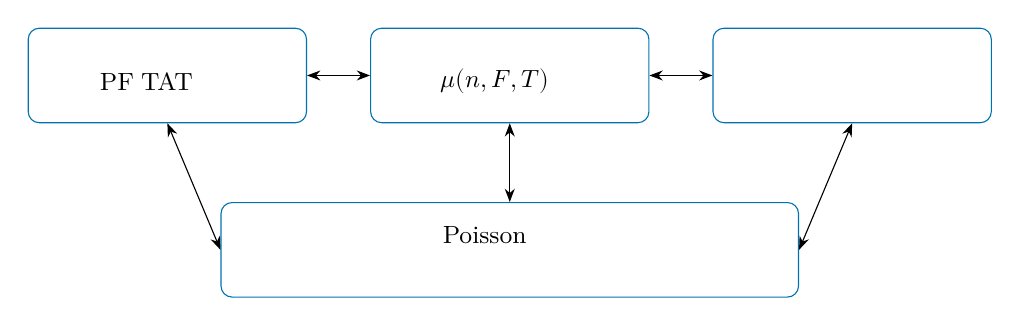
\begin{tikzpicture}[node distance=8mm,box/.style={draw=tolblue,rounded corners,align=center,text width=3.3cm,minimum height=1.2cm,font=\small},>=Stealth]
\node[box](g){{\cjkfont 产生与复合}\allowbreak{}\\PF{\cjkfont 、}\allowbreak{}TAT{\cjkfont 、供受体循环}\allowbreak{}};
\node[box,right=of g](t){{\cjkfont 无序跳跃输运}\allowbreak{}\\$\mu(n,F,T)$ {\cjkfont 与扩散}\allowbreak{}};
\node[box,right=of t](c){{\cjkfont 电极边界}\allowbreak{}\\{\cjkfont 注入、抽取、界面占据}\allowbreak{}};
\draw[<->](g)--(t);\draw[<->](t)--(c);
\node[box,below=10mm of t,text width=7.1cm](p){Poisson {\cjkfont 与连续性方程}\allowbreak{}\\{\cjkfont 电场、占据、准费米能级和电流共同求解}\allowbreak{}};
\draw[<->](g.south)--(p.west);\draw[<->](t)--(p);\draw[<->](c.south)--(p.east);
\end{tikzpicture}
\caption{{\cjkfont 共同器件框架的概念示意。箭头表示自洽反馈，不代表可直接相加的独立电流。图不包含材料拟合结果。}\allowbreak{}}\label{fig:common-framework}
\end{figure}

\subsection{{\cjkfont 从高斯态密度到载流子占据}\allowbreak{}}
{\cjkfont 无序材料中，不同局部环境对应不同位点能量。作为可检验的工作近似，对电子或空穴输运流形分别使用高斯态密度}\allowbreak{}
\begin{equation}
 g(\varepsilon)=\frac{N}{\sqrt{2\pi}\sigma}\exp\!\left[-\frac{(\varepsilon-\varepsilon_0)^2}{2\sigma^2}\right],\qquad
 n=\int g(\varepsilon)f(\varepsilon,E_F,T)\,d\varepsilon .
\end{equation}
{\cjkfont 这里}\allowbreak{} $N$ {\cjkfont 是位点密度，}\allowbreak{}$\sigma$ {\cjkfont 是能量无序宽度，}\allowbreak{}$E_F$ {\cjkfont 为局域准费米能级。电子的}\allowbreak{} $f$ {\cjkfont 取}\allowbreak{} Fermi {\cjkfont 占据；空穴采用相应空态占据和一致的能量符号。单一平均能级的占据率不能替代整个}\allowbreak{} DOS {\cjkfont 的积分。}\allowbreak{}

{\cjkfont 低密度时，载流子倾向占据深尾态，离开这些态需要较大的热激活代价。密度增加时，深尾态被部分填满，可参与输运的能量窗口改变。因而迁移率可以依赖密度；但这不意味着载流子必须在同一时刻占据一条连续分子链。电流是随时间发生的跳跃序列，路径瓶颈取决于能量、距离、占据和网络连通性。}\allowbreak{}

{\cjkfont 将}\allowbreak{} $N=a^{-3}$ {\cjkfont 用于规则格点模型时，}\allowbreak{}$a$ {\cjkfont 是该模型的位点间距。它不应同时被随意解释为化学分子直径、真实相区尺度、陷阱到受体的跃迁距离或所有模型共用的拟合长度。}\allowbreak{}

\subsection{{\cjkfont 迁移率与扩散必须使用同一统计闭合}\allowbreak{}}
{\cjkfont 本轮体输运采用}\allowbreak{} Pasveer {\cjkfont 等的高斯无序迁移率参数化，写为}\allowbreak{}
\begin{equation}
 \mu(n,F,T)=\mu_*\exp[-0.42s^2]g_1(c,s)g_2(u,s),\qquad
 s=\frac{\sigma}{k_BT},\quad c=na^3,\quad u=\frac{q|F|a}{\sigma}.
\end{equation}
$\mu_*$ {\cjkfont 为温度无关的前因子；采用}\allowbreak{} SI {\cjkfont 能量单位时}\allowbreak{} $u$ {\cjkfont 中显式包含}\allowbreak{} $q${\cjkfont 。原参数化的密度与场因子为}\allowbreak{}
\begin{align}
 g_1&=\exp\!\left[\tfrac12(s^2-s)(2c)^\delta\right], &
 \delta&=\frac{2\{\ln(s^2-s)-\ln(\ln4)\}}{s^2},\\
 g_2&=\exp\!\left[0.44(s^{3/2}-2.2)\bigl(\sqrt{1+0.8u^2}-1\bigr)\right].
\end{align}
{\cjkfont 这些式子是对规定无序格点主方程结果的参数化，不是任意材料、任意占据和电场下的定理。我们使用的文献比较窗口约为}\allowbreak{} $2\le s\le6${\cjkfont 、}\allowbreak{}$10^{-6}\le c\le10^{-2}${\cjkfont 。原图场范围到}\allowbreak{} $u\simeq3${\cjkfont ；图覆盖范围不能解释成普适有效性边界。高占据接触区尤其需要单独审查。}\allowbreak{}

{\cjkfont 相同}\allowbreak{} DOS {\cjkfont 的热力学压缩率同时决定广义}\allowbreak{} Einstein {\cjkfont 关系：}\allowbreak{}
\begin{equation}
 \frac{D}{\mu}=\frac{n}{q(\partial n/\partial E_F)_T}.
\end{equation}
{\cjkfont 此式中}\allowbreak{} $E_F$ {\cjkfont 以焦耳计。稀薄}\allowbreak{} Boltzmann {\cjkfont 极限恢复}\allowbreak{} $D/\mu=k_BT/q${\cjkfont 。在有限占据时，如果只修改迁移率而仍无条件使用稀薄}\allowbreak{} Einstein {\cjkfont 关系，就会把不同统计假设拼在一起。这里的关系仍依赖局域准平衡，强场下这一前提本身要检查。}\allowbreak{}

{\cjkfont 数值上使用逆活度型广义}\allowbreak{} Scharfetter--Gummel {\cjkfont 通量，并分别检查电子和空穴的符号。等准费米能级时电流精确为零、各面电流守恒，是最低要求；这些要求不等于接触模型已经真实。}\allowbreak{}

\begin{figure}[htbp]\centering
\includegraphics[width=.97\linewidth]{figures/temperature_transport_benchmark.png}
\caption{{\cjkfont 独立输运模块对已发表}\allowbreak{} Pasveer {\cjkfont 参数化的复现。它展示温度、占据与场的联合作用；不是重新计算原论文三维主方程数据，也不是}\allowbreak{} D18:L8-BO {\cjkfont 实测迁移率。}\allowbreak{}}\label{fig:transport-temperature-benchmark}
\end{figure}

\subsection{{\cjkfont 为什么端电流激活能不等于产生势垒}\allowbreak{}}
{\cjkfont 定义某一可观测量的局部表观激活能为}\allowbreak{}
\begin{equation}
 E_{a,\mathrm{app}}=-k_B\frac{\partial\ln |J|}{\partial(1/T)}.
\end{equation}
{\cjkfont 导数必须说明保持什么不变。固定端电压、固定平均场和固定局部场不是同一实验；随温度变化的空间电荷和接触势垒会重分配内部电压。}\allowbreak{}

{\cjkfont 在供给限制且充分收集的理想稳态极限，}\allowbreak{}$J\simeq q\int G\,dx${\cjkfont 。此时迁移率变化可以主要改变密度和渡越时间，而未必同比例改变电流。存在复合、有限抽取或空间电荷时，可形式上写出}\allowbreak{} $J\simeq qdG\eta_{\mathrm{coll}}${\cjkfont ，进而温度导数包含产生与收集两部分。这个分解也只有在均匀近似、分支定义明确且没有额外注入或倍增时才成立；一般器件应直接使用连续性分账。}\allowbreak{}

{\cjkfont 即便只看低密度低场迁移率，}\allowbreak{}$\ln\mu=\ln\mu_*-0.42(\sigma/k_BT)^2$ {\cjkfont 也不是恒定势垒的}\allowbreak{} Arrhenius {\cjkfont 直线。其局部温度导数对应}\allowbreak{} $E_{a,\mu}=0.84\sigma^2/(k_BT)${\cjkfont 。因此}\allowbreak{}“{\cjkfont 斜率随}\allowbreak{} $1/T$ {\cjkfont 变化}\allowbreak{}”{\cjkfont 不能单独证明某个产生机制是跳跃。}\allowbreak{}

{\cjkfont 经典}\allowbreak{} Marcus {\cjkfont 单步速率含}\allowbreak{} $T^{-1/2}$ {\cjkfont 前因子，且势垒为}\allowbreak{} $(\lambda+\Delta G)^2/(4\lambda)${\cjkfont 。若}\allowbreak{} $\Delta G$ {\cjkfont 包含线性场做功，势垒通常对场呈二次函数，只在有限场窗内近似线性。}\allowbreak{}MLJ {\cjkfont 多振动态求和、}\allowbreak{}DOS {\cjkfont 积分及速率串联会进一步改变表观斜率。}\allowbreak{}PF {\cjkfont 的热发射也可有很强的温度依赖；}\allowbreak{}CT {\cjkfont 场解离并不普遍等同于}\allowbreak{} Coulomb PF{\cjkfont 。不同机制的简短线性作图规则只能用作受限模型检查。}\allowbreak{}

\subsection{{\cjkfont 补充图}\allowbreak{} S10 {\cjkfont 提供了怎样的文献约束}\allowbreak{}}
Huang {\cjkfont 等补充图}\allowbreak{} S10 {\cjkfont 给出了}\allowbreak{} PM6:BTP-eC9 {\cjkfont 在}\allowbreak{} 300{\cjkfont 、}\allowbreak{}340{\cjkfont 、}\allowbreak{}380{\cjkfont 、}\allowbreak{}420 K {\cjkfont 的反向}\allowbreak{} $J$--$V${\cjkfont 。此前认为论文没有可用固定偏压变温电流的判断需要修正。我们对原图做了颜色、坐标和线宽核验后的数字化，结果见表。它们是读图估计，不是作者原始数据，也不是当前}\allowbreak{} D18:L8-BO {\cjkfont 样品的测量。}\allowbreak{}

\begin{table}[htbp]\centering\small
\begin{tabular}{rrrr}\toprule
$T$ (K)&$J(-5\,\mathrm V)$&$J(-10\,\mathrm V)$&$J(-15\,\mathrm V)$\\\midrule
300&0.029&0.123&0.424\\
340&0.111&0.438&1.36\\
380&0.257&1.00&2.90\\
420&1.07&3.69&10.0\\\bottomrule
\end{tabular}
\caption{S10 {\cjkfont 数字化的电流密度绝对值，单位为}\allowbreak{} $\mathrm{mA\,cm^{-2}}${\cjkfont 。所设像素误差包络约为}\allowbreak{} $-13\%$ {\cjkfont 至}\allowbreak{} $+15\%${\cjkfont ，不包含实验误差、温标、自热和样品差异。}\allowbreak{}}
\end{table}

{\cjkfont 四点描述性}\allowbreak{} Arrhenius {\cjkfont 拟合得到约}\allowbreak{} $0.314${\cjkfont 、}\allowbreak{}$0.297${\cjkfont 、}\allowbreak{}$0.276$ eV{\cjkfont ；读图包络分别约}\allowbreak{} $\pm0.029${\cjkfont 、}\allowbreak{}$\pm0.027${\cjkfont 、}\allowbreak{}$\pm0.027$ eV{\cjkfont ，不能当作统计置信区间。从}\allowbreak{} $-5$ {\cjkfont 到}\allowbreak{} $-15$ V {\cjkfont 的差值不足以单独证明激活能随场线性下降。最高温段有更大的两点斜率，提示单一}\allowbreak{} Arrhenius {\cjkfont 描述不充分；只有四个温度且缺少重复测量，不能据此宣布机制转变。}\allowbreak{}

\begin{figure}[htbp]\centering
\includegraphics[width=.97\linewidth]{figures/S10_temperature_digitization.png}
\caption{S10 {\cjkfont 端电流的温度读图及曲率检查。固定的是端电压；该组器件厚度尚未核实，故不换算为固定局部电场。图中的误差来自指定像素包络。}\allowbreak{}}\label{fig:S10-temperature}
\end{figure}

\subsection{{\cjkfont 已经完成的器件控制与暴露的问题}\allowbreak{}}
{\cjkfont 示例使用}\allowbreak{} $\sigma_n=\sigma_p=0.1$ eV{\cjkfont 、}\allowbreak{}$a=1$ nm{\cjkfont 、}\allowbreak{}$N=10^{21}\,\mathrm{cm^{-3}}${\cjkfont ；}\allowbreak{}300 K {\cjkfont 零密度零场迁移率锚到旧基线，仅为受控比较。它们不是目标材料测量参数。所有温度共用参数，没有逐温度拟合。旧模型的态密度为}\allowbreak{} $10^{19}\,\mathrm{cm^{-3}}${\cjkfont ，故完整更换}\allowbreak{} DOS {\cjkfont 后的变化不能全归因于迁移率。}\allowbreak{}

{\cjkfont 已比较旧单能级恒迁移率、仅加入温度迁移率、}\allowbreak{}Gaussian DOS {\cjkfont 冻结迁移率，以及}\allowbreak{} Gaussian DOS {\cjkfont 与完整}\allowbreak{} $\mu(n,F,T)$ {\cjkfont 四组。单独输运示例在固定}\allowbreak{} $n=10^{16}\,\mathrm{cm^{-3}}${\cjkfont 、}\allowbreak{}$F=10^5\,\mathrm{V\,cm^{-1}}$ {\cjkfont 下，}\allowbreak{}420/300 K {\cjkfont 的迁移率比约为}\allowbreak{} 17.6{\cjkfont ；这一比值并不自动成为器件电流比。}\allowbreak{}

{\cjkfont 空间细化给出了决定性的警告：}\allowbreak{}300 K {\cjkfont 完整}\allowbreak{} Gaussian {\cjkfont 器件的}\allowbreak{} 161 {\cjkfont 到}\allowbreak{} 321 {\cjkfont 节点变化在已测反偏点不超过}\allowbreak{} 0.92\%{\cjkfont ，}\allowbreak{}420 K {\cjkfont 却仍变化}\allowbreak{} 43--45\%{\cjkfont 。因此粗网格完整器件的激活能和所谓}\allowbreak{}“{\cjkfont 迁移率使电流增加}\allowbreak{} 54--64\%”{\cjkfont 不再用于定量解释。}\allowbreak{}

420 K{\cjkfont 、}\allowbreak{}$-5$ V {\cjkfont 时，非局域净产生约}\allowbreak{} $0.504\,\mu\mathrm{A\,cm^{-2}}${\cjkfont 、双分子热产生约}\allowbreak{} $8.07\,\mu\mathrm{A\,cm^{-2}}$ {\cjkfont 已近稳定，但单端接触注入随细网格从}\allowbreak{} 2.84 {\cjkfont 增至}\allowbreak{} 7.58{\cjkfont 、再到}\allowbreak{} $16.6\,\mu\mathrm{A\,cm^{-2}}${\cjkfont 。接触占据约为三分之一，远超过低密度拟合窗；最大}\allowbreak{} $qFa/\sigma$ {\cjkfont 从}\allowbreak{} 1.69 {\cjkfont 增至}\allowbreak{} 3.39{\cjkfont 。由}\allowbreak{} DOS {\cjkfont 压缩率估算的屏蔽长度约}\allowbreak{} 0.25 nm{\cjkfont ，小于假设分子间距}\allowbreak{} 1 nm{\cjkfont 。继续把连续介质网格细化到亚分子尺度，不能解决物理模型的层级问题。}\allowbreak{}

{\cjkfont 冻结迁移率的接触控制在}\allowbreak{} 161{\cjkfont 、}\allowbreak{}321{\cjkfont 、}\allowbreak{}641 {\cjkfont 节点给出}\allowbreak{} 8.727{\cjkfont 、}\allowbreak{}8.786{\cjkfont 、}\allowbreak{}$8.820\,\mu\mathrm{A\,cm^{-2}}${\cjkfont ，末次变化}\allowbreak{} 0.386\%{\cjkfont 。这支持问题集中在未验证的接触输运闭合，但不能证明恒迁移率替代真实。}\allowbreak{}

{\cjkfont 已通过的检查包括模块积分、正反详细平衡、平衡零电流、通量符号、制造解空间收敛及保存状态的电荷}\allowbreak{}/{\cjkfont 电流}\allowbreak{}/{\cjkfont 能量核验。它们证明所写方程被一致处理，不证明参数已标定或所有器件预测均已收敛。}\allowbreak{}

\subsection{{\cjkfont 高占据微观边界基准与局限}\allowbreak{}}
{\cjkfont 为避免把低密度经验迁移率外推到接触高占据区，我们建立了一个独立的分子尺度边界基准。它包含}\allowbreak{} 8 {\cjkfont 个位点、全部}\allowbreak{} $2^8=256$ {\cjkfont 个排斥占据构型、}\allowbreak{}Gaussian {\cjkfont 随机裸能级、}\allowbreak{}Miller--Abrahams {\cjkfont 双向跳跃和有限速率双向电极交换。每条跃迁使用完整构型的能量差，而非只用平均占据的静电势。电子占据限制与相关性因此被显式保留。}\allowbreak{}

{\cjkfont 模型的固定电极势热力学势为}\allowbreak{}
\begin{equation}
 U(\boldsymbol n)=\sum_i n_i(\varepsilon_i-q\phi_{\mathrm{ext},i})+
 \frac{q^2a}{2\epsilon A}(\boldsymbol n-\boldsymbol b)^T
 L^{-1}(\boldsymbol n-\boldsymbol b).
\end{equation}
{\cjkfont 这里以焦耳计能量，}\allowbreak{}$L$ {\cjkfont 为无量纲}\allowbreak{} Dirichlet {\cjkfont 离散}\allowbreak{} Laplace {\cjkfont 矩阵，}\allowbreak{}$a=1$ nm{\cjkfont 、}\allowbreak{}$A=4$ nm$^2${\cjkfont ，电极间长度为}\allowbreak{} 9 nm{\cjkfont 。固定正补偿背景每站为}\allowbreak{} $b=0.3$ {\cjkfont 个元电荷。这是平面电容链的假想几何，不能当成三维分子之间精确的}\allowbreak{} $1/r$ {\cjkfont 势，也不是样品已知掺杂。电压源作用已经包含在构型势中，跃迁时不能再加第二份场做功。}\allowbreak{}

{\cjkfont 保持参数和无序不变，计算}\allowbreak{} 12 {\cjkfont 组无序、}\allowbreak{}4 {\cjkfont 个温度和}\allowbreak{} 2 {\cjkfont 个平均外加场，共}\allowbreak{} 96 {\cjkfont 个工况，另作}\allowbreak{} 26 {\cjkfont 个条件控制。已完成稳态概率、截面粒子流、正反详细平衡、}\allowbreak{}Gauss {\cjkfont 电荷和功热关系的核验及独立复核。这个系统只有一种载流子，没有电子}\allowbreak{}--{\cjkfont 空穴成对产生、复合或热失控。}\allowbreak{}

\begin{figure}[htbp]\centering
\includegraphics[width=.97\linewidth]{figures/temperature_exclusion_benchmark.pdf}
\caption{{\cjkfont 有限排斥跳跃链的温度反例。每条链电流幅值按自身}\allowbreak{} 300 K {\cjkfont 归一化；固定的是外加平均场。所有非温度参数均固定。它不是器件}\allowbreak{} J--V{\cjkfont ，也没有与实验电流幅值拟合。}\allowbreak{}}\label{fig:exclusion-temperature}
\end{figure}

{\cjkfont 在}\allowbreak{} $0.5\,\mathrm{MV\,cm^{-1}}$ {\cjkfont 下，各链的}\allowbreak{} $|J(420)|/|J(300)|$ {\cjkfont 从}\allowbreak{} 1.09 {\cjkfont 到}\allowbreak{} 111.6{\cjkfont ；在}\allowbreak{} $1.5\,\mathrm{MV\,cm^{-1}}$ {\cjkfont 下，}\allowbreak{}12 {\cjkfont 条链中有}\allowbreak{} 10 {\cjkfont 条落在}\allowbreak{} 0.9625--1.0115{\cjkfont ，另外两条为}\allowbreak{} 4.22 {\cjkfont 和}\allowbreak{} 6.51{\cjkfont 。纯跳跃也能给出几乎平坦、甚至略下降的端电流：高场使部分前向跃迁进入下坡速率上限，而逆向过程、占据和电极交换仍在变化。由此可严格否定}\allowbreak{}“{\cjkfont 弱温度依赖足以证明弹性隧穿}\allowbreak{}”{\cjkfont 这一单独判据；不能据样本比例判断宏观薄膜机制。}\allowbreak{}

{\cjkfont 这项反例也有明确假设。有效最近邻时钟取恒定}\allowbreak{} $10^9\,\mathrm{s^{-1}}${\cjkfont ，已吸收固定距离衰减，并非真实材料的温度无关前因子测量。关闭电容相互作用的排斥链仍可给出约}\allowbreak{} 0.955 {\cjkfont 的温度比，说明弱温度反例并不完全依赖补偿背景。然而保留充电而删除背景会引发极强阻塞，显著改变绝对电流。背景、电容和几何不能作为隐蔽的拟合自由度。}\allowbreak{}

\begin{figure}[htbp]\centering
\includegraphics[width=.97\linewidth]{figures/contact_occupancy_controls.pdf}
\caption{{\cjkfont 微观接触控制展示交换速率、占据和充电假设的影响。改变位点数改变物理长度与无序片段，不是同一器件的数值网格细化。绝对电流由假定通道面积与时钟决定，不能与实际暗电流直接比较。}\allowbreak{}}\label{fig:contact-occupancy-control}
\end{figure}

{\cjkfont 该基准证明可在有限高占据系统中避免}\allowbreak{} EGDM {\cjkfont 外推，同时保留详细平衡与电荷守恒。它尚未修复前述}\allowbreak{} 100 nm {\cjkfont 器件，也没有建立三维无序平均或宏观尺寸收敛。下一步必须处理微观接触区与连续体体相的化学势、通量和电荷匹配，不能把有限链电流直接作为新的体产生率。}\allowbreak{}

\subsection{{\cjkfont 接下来如何比较产生与接触机制}\allowbreak{}}
{\cjkfont 第一步是使接触和体输运各自处于可解释的范围，保留}\allowbreak{} Gaussian DOS{\cjkfont 、占据统计、扩散及局部场反馈的一致性。不能用无依据的迁移率截断掩盖高场外推，也不能改变注入势垒把曲线凑到}\allowbreak{} S10{\cjkfont 。}\allowbreak{}

{\cjkfont 第二步，在相同温度、厚度、无序和接触参数下，只更换有明确状态定义的产生循环，逐一报告每步速率、净产生、复合损失、接触净供给和端电流。对非局域转移还应保留两端源项与相应内部电流；不能把微观净跨窗电流再当成本地产生重复加入。}\allowbreak{}

{\cjkfont 第三步，以端口}\allowbreak{} $J(V,T)$ {\cjkfont 检查文献对应，同时把局域产生的温度导数与收集、输运、接触的贡献分开。室温仍是当前基线；低温用于后续区分机制，但需要同时检查跳跃参数化和局域准平衡的适用性。}\allowbreak{}

{\cjkfont 本章支持采用无序跳跃输运作为共同起点，尚不支持宣布}\allowbreak{} PF{\cjkfont 、}\allowbreak{}Marcus/MLJ{\cjkfont 、陷阱辅助隧穿或接触路线中的任何一条已被实验证实。模型之间最有价值的比较，是同样严格的守恒与参数约束下，哪些路线能够同时解释幅值、温度、厚度和接触改变，哪些路线在完整循环或边界处失败。}\allowbreak{}

\subsection{{\cjkfont 本章主要来源}\allowbreak{}}
\begin{enumerate}
\item Pasveer et al., Unified Description of Charge-Carrier Mobilities in Disordered Semiconducting Polymers, Physical Review Letters 94, 206601 (2005). \url{https://doi.org/10.1103/PhysRevLett.94.206601}.
\item Roichman and Tessler, Generalized Einstein relation for disordered semiconductors. \url{https://arxiv.org/abs/cond-mat/0109432}.
\item Doan, Glitzky and Liero, WIAS Preprint 2493 (2018). \url{https://doi.org/10.20347/WIAS.PREPRINT.2493}. {\cjkfont 本章参考其无序输运热力学闭合和逆活度离散。}\allowbreak{}
\item Huang et al., Perovskite--organic tandem solar cells with superior reverse-bias stability, Nature Materials (2026). \url{https://doi.org/10.1038/s41563-026-02541-6}. {\cjkfont 本章温度数据来自补充图}\allowbreak{} S10{\cjkfont ，不能与损坏阈值}\allowbreak{} $V_{\rm RB}$ {\cjkfont 混为同一观测量。}\allowbreak{}
\item Miller and Abrahams, Physical Review 120, 745 (1960). \url{https://doi.org/10.1103/PhysRev.120.745}. {\cjkfont 有限链采用其上坡热激活、下坡固定时钟的速率形式。}\allowbreak{}
\item Novikov, Hopping transport of interacting carriers in disordered organic materials. \url{https://arxiv.org/abs/0708.4313}. {\cjkfont 参考其对相互作用和动态相关的讨论；本章未复现该文的材料计算。}\allowbreak{}
\end{enumerate}
\FloatBarrier
\clearpage

% ===== FROZEN SECTION 3 =====
\clearpage
\part*{{\cjkfont 第一部分}\allowbreak{} \allowbreak{}{\cjkfont 从电子态到器件}\allowbreak{}}
\FloatBarrier
\Needspace{110pt}
\section{{\cjkfont 无机能带图为何不能原样搬过来}\allowbreak{}}\label{sec:3}
% SOURCE 3-paragraph-0 a834e5d8b3b3604dc99a387c0ee6591e0f07b7ad9ecd1513a080d600cb9f3cb8
{\cjkfont 理想晶体中，电子受到周期势作用，能用}\allowbreak{}Bloch\allowbreak{}{\cjkfont 态、能带色散和有效质量组织输运问题。波包在两次散射之间可以在动量空间被电场加速；在特定场强、平均自由程和能带条件下，热载流子、带间隧穿或碰撞电离成为合适的描述。晶体中的缺陷则在这个延展态背景上引入局域能级。}\allowbreak{}
\par
% SOURCE 3-paragraph-1 1a453d183f3d41d38145c555204c7a60a2ed5b81abe7675241b621944515e75d
{\cjkfont 分子有机半导体仍有轨道和能量分布，但分子间耦合、构象、侧链、晶域与非晶区会改变态的空间范围。电荷可能在一个分子或有限片段上局域，并伴随周围分子的电子极化与核坐标重排。因此，“}\nobreak{}HOMO/LUMO\nobreak{}{\cjkfont ”不是一张自动包含输运有效质量、迁移率和缺陷截面的连续能带图。}\allowbreak{}
\par
% SOURCE 3-paragraph-2 24a86d205bd376f5580571b412f8f09968468d60604b77208b57847d6b460942
{\cjkfont 这不是说有机材料绝不具有离域态或带样输运。不同纯度、温区、堆积和时间尺度可以处于不同极限。正确的做法是先确定所研究过程使用的态与长度尺度，再决定是否能采用带输运、局域跳跃或两者结合。把本项目称为有机半导体，不能替代这一步判断。}\allowbreak{}
\par
% SOURCE 3-paragraph-3 9195914da7a531b09fba6568084568d0ef66a0ebc0850a03c1a3f0ae1eed630b
{\cjkfont 反偏问题尤其敏感：能在原子级局部发生的快速跃迁，未必能把载流子穿过}\allowbreak{}100 nm\allowbreak{}{\cjkfont 薄膜；能在晶域内移动的电子，未必跨得过给受体界面或再次填满一个缺陷。微观转移与宏观连续性必须接起来。}\allowbreak{}
\par
\begin{figure}[!htbp]
\centering
\resizebox{.90\linewidth}{!}{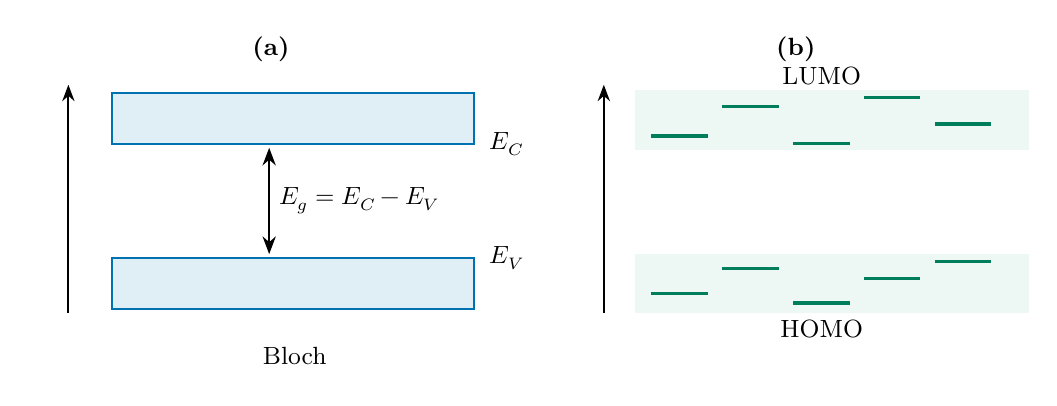
\begin{tikzpicture}[x=1cm,y=1cm,box/.style={draw=tolblue,fill=tolblue!4,line width=.8pt,align=center,inner sep=8pt,font=\small},bi/.style={<->,>=Stealth,line width=.85pt,draw=tolblue}]

% Conceptual electronic energy layout: no measured organic energy or gap.
\node[font=\small\bfseries]at(2.35,3.3){(a) {\cjkfont 周期无机晶体}};
\node[font=\small\bfseries]at(9.15,3.3){(b) {\cjkfont 典型无序有机半导体}};
\draw[-{Stealth},line width=.65pt](-.55,-.05)--(-.55,2.85);
\node[rotate=90,font=\small]at(-.95,1.4){{\cjkfont 电子能量}};
\draw[fill=tolblue!12,draw=tolblue,line width=.8pt](0,2.1)rectangle(4.6,2.75);
\draw[fill=tolblue!12,draw=tolblue,line width=.8pt](0,0)rectangle(4.6,.65);
\node[font=\small]at(2.3,2.43){{\cjkfont 导带：延展态}};
\node[font=\small]at(2.3,.33){{\cjkfont 价带：延展态}};
\node[anchor=west,font=\small]at(4.68,2.1){$E_C$};
\node[anchor=west,font=\small]at(4.68,.65){$E_V$};
\draw[<->,>=Stealth,line width=.75pt](2.0,.70)--node[right,font=\small]{$E_g=E_C-E_V$}(2.0,2.05);
\node[font=\small]at(2.3,-.6){{\cjkfont 周期势}\quad Bloch{\cjkfont 态与能带色散}};
\draw[-{Stealth},line width=.65pt](6.25,-.05)--(6.25,2.85);
% Shaded envelopes mark disorder spread, not a continuous Bloch band.
\fill[tolgreen!7](6.65,-.05)rectangle(11.65,.70);
\fill[tolgreen!7](6.65,2.02)rectangle(11.65,2.78);
\foreach \x/\y in {6.85/2.20,7.75/2.57,8.65/2.10,9.55/2.69,10.45/2.35}{
 \draw[draw=tolgreen!80!black,line width=1.2pt](\x,\y)--++(.72,0);
}
\foreach \x/\y in {6.85/.20,7.75/.52,8.65/.08,9.55/.39,10.45/.61}{
 \draw[draw=tolgreen!80!black,line width=1.2pt](\x,\y)--++(.72,0);
}
\node[font=\small]at(9.15,2.96){LUMO{\cjkfont 衍生态}};
\node[font=\small]at(9.15,-.25){HOMO{\cjkfont 衍生态}};
\node[font=\small,align=center]at(9.15,1.40){{\cjkfont 能量与空间分布依赖局部环境}\\{\cjkfont 短线：不同分子或有限片段的态}};
\node[font=\small]at(9.15,-.75){{\cjkfont 局域态与有限离域}\quad {\cjkfont 重组、跳跃与连通性}};
\end{tikzpicture}}
\caption{{\cjkfont 无机能带与典型无序}\allowbreak{}OSC\allowbreak{}{\cjkfont 能级的概念对照。左为周期晶体的价带、导带及带隙；右为}\allowbreak{}HOMO/LUMO\allowbreak{}{\cjkfont 衍生态，不同短线表示不同局部环境的态能，浅色区仅提示无序展宽，不代表连续}\allowbreak{}Bloch\allowbreak{}{\cjkfont 能带。横向排布不对应波矢或实测距离。有机态可局域于分子或有限片段，也可有限离域；该图不排除有序有机材料中的带样输运。两图能量零点和间距均任意，不是}\allowbreak{}D18:L8-BO\allowbreak{}{\cjkfont 实测能级，也未给出光学隙或输运隙数值。}\allowbreak{}}\label{fig:1}
{\footnotesize\color{SourceGray} {\cjkfont 理论背景}\allowbreak{} \cite{R1} \cite{R5} \cite{R6}\par}
\end{figure}
\medskip
% ===== FROZEN SECTION 4 =====
\clearpage
\begin{landscape}
\phantomsection\addcontentsline{toc}{section}{{\cjkfont 晶硅 有机与钙钛矿的反偏比较}}
\begin{center}
{\large\bfseries {\cjkfont 晶硅}\allowbreak{} \allowbreak{}{\cjkfont 有机与卤化物钙钛矿太阳能电池的反偏比较}\allowbreak{}\par}
\vspace{5pt}
{\fontsize{10.5}{14}\selectfont {\cjkfont 电流上翘、强反向导电与永久损伤须区分；文献电压实例不是普适阈值。温度比较使用反向电压绝对值，并固定判据。}\allowbreak{}\par}
\end{center}
\begingroup\fontsize{10.5}{14}\selectfont\setstretch{1}\renewcommand{\arraystretch}{1.05}
\setlength{\tabcolsep}{6pt}
\begin{tabular}{@{}>{\raggedright\arraybackslash}p{22mm}>{\raggedright\arraybackslash}p{66mm}>{\raggedright\arraybackslash}p{66mm}>{\raggedright\arraybackslash}p{66mm}@{}}
\toprule
\textbf{{\cjkfont 比较项}\allowbreak{}} & \textbf{{\cjkfont 晶硅}\allowbreak{}} & \textbf{{\cjkfont 有机}\allowbreak{} \allowbreak{}{\cjkfont 无序体异质结为主}\allowbreak{}} & \textbf{{\cjkfont 卤化物钙钛矿}\allowbreak{}}\\\midrule
{\cjkfont 主要机制}\allowbreak{} & {\cjkfont 雪崩倍增；高掺杂窄结可有带间隧穿；缺陷和局部高场可提前导通}\allowbreak{} [C1,C2] & {\cjkfont 候选为接触注入}\allowbreak{}/\allowbreak{}{\cjkfont 隧穿、陷阱辅助或其他场增强产生、局部弱区导电。本项目机制尚未确定}\allowbreak{} [C3] & {\cjkfont 离子再分布改变界面场；叠加注入}\allowbreak{}/\allowbreak{}{\cjkfont 隧穿、电化学反应和局部热效应}\allowbreak{} [C5,C6]\\[5pt]
{\cjkfont 输运特点}\allowbreak{} & {\cjkfont 以能带输运为主；雪崩需满足碰撞电离条件，不能仅凭“自由程长”判断}\allowbreak{} & {\cjkfont 常用局域态跳跃描述，受无序、占据及形貌连通性控制；跳距不等于能带自由程}\allowbreak{} [C4] & {\cjkfont 电子}\allowbreak{}/\allowbreak{}{\cjkfont 空穴输运与可移动离子并存；离子改变场、势垒和化学状态}\allowbreak{}\\[5pt]
{\cjkfont 触发场和电压}\allowbreak{} & {\cjkfont 取决于掺杂、耗尽层、结曲率与缺陷；局部提前导通不等于理想均匀结击穿}\allowbreak{} & 10 V \allowbreak{}{\cjkfont 若全落在}\allowbreak{} 100 nm \allowbreak{}{\cjkfont 层上，平均场为}\allowbreak{} 1 MV/cm\nobreak{}{\cjkfont ，非普适阈值。优化}\allowbreak{} OSC \allowbreak{}{\cjkfont 有不可逆击穿}\allowbreak{} \ensuremath{\vert}V\ensuremath{\vert}\ensuremath{>}35 V \allowbreak{}{\cjkfont 的报道}\allowbreak{} [C3] & {\cjkfont 特定早期器件为}\allowbreak{} −1 \allowbreak{}{\cjkfont 至}\allowbreak{} −4 V [C5]\nobreak{}{\cjkfont ；优化阻挡层已有}\allowbreak{} \ensuremath{\vert}Vbd\ensuremath{\vert}\ensuremath{>}20 V [C6]\nobreak{}{\cjkfont ，不宜给统一范围}\allowbreak{}\\[5pt]
{\cjkfont 温度依赖}\allowbreak{} & {\cjkfont 理想雪崩主导时}\allowbreak{} \ensuremath{\vert}Vbd\ensuremath{\vert} \allowbreak{}{\cjkfont 通常随温度升高而增大；}\allowbreak{}Zener \allowbreak{}{\cjkfont 主导者可减小，混合机制另判}\allowbreak{} [C1] & {\cjkfont 发射}\allowbreak{}/\allowbreak{}{\cjkfont 注入与隧穿响应不同；固定电流阈值和形状膝点不可混用。本项目尚无变温定论}\allowbreak{} & {\cjkfont 离子、反应和电子过程共同影响；表观阈值也随测试时长及预处理而变}\allowbreak{}\\[5pt]
{\cjkfont 时间和历史依赖}\allowbreak{} & {\cjkfont 电子响应可快，但自热、缺陷演化和应力损伤会产生历史依赖}\allowbreak{} [C2] & {\cjkfont 本项目：扫描快慢及是否脉冲对膝点影响不明显；脉宽等待补齐，不能泛化为所有器件}\allowbreak{} & {\cjkfont 常有明显偏压历史、保持时间和扫描程序影响；程度依结构及条件而变}\allowbreak{} [C5,C6]\\[5pt]
{\cjkfont 损伤与可逆性}\allowbreak{} & {\cjkfont 局部电流可形成热点并永久损伤；反向导电开始不等于已损坏}\allowbreak{} & {\cjkfont 本项目：轻微越过膝点后，正向}\allowbreak{} J–V \allowbreak{}{\cjkfont 基本不变，反扫可重现。更强应力的永久损伤机制另查}\allowbreak{} & {\cjkfont 可有可恢复变化或永久短路、金属丝、腐蚀与分解；不保证一律“先软后硬”}\allowbreak{} [C5,C6]\\[5pt]
{\cjkfont 常见缓解方向}\allowbreak{} & {\cjkfont 旁路保护、控制缺陷和局部场集中、改善散热并验证耐受性}\allowbreak{} & {\cjkfont 改善膜厚}\allowbreak{}/\allowbreak{}{\cjkfont 形貌均匀性、接触选择性及阻挡层，配合限流；措施需匹配机制}\allowbreak{} & {\cjkfont 离子}\allowbreak{}/\allowbreak{}{\cjkfont 金属阻挡层、稳定接触与传输层、减少局部缺陷电流并配合模块保护}\allowbreak{} [C6]\\[5pt]
\bottomrule\end{tabular}\par\endgroup
\noindent\vspace{6pt}{\fontsize{9.5}{12}\selectfont {\cjkfont 本项目观察来自用户陈述，尚未逐项核对原始曲线和脉冲波形。实际局部电场需自洽求解；银迁移不是本器件已证实的损伤机制。资料索引见下一页。}\allowbreak{}\par}\end{landscape}\clearpage
\subsection*{{\cjkfont 比较表的来源与使用边界}\allowbreak{}}
{\cjkfont 这张表用于建立候选机制和测量尺度的比较，不用于仅凭端电压、温度趋势或曲线形状给器件定性。特别是本项目已报告轻微越过膝点具有可重复性，应先解释可逆的电流上翘，再单独研究更强应力引发的损伤。}\allowbreak{}\par\medskip
\noindent [C1] M. Singh Tyagi (1968). Zener and avalanche breakdown in silicon alloyed p–n junctions—II. Solid-State Electronics 11, 117–128. DOI: \href{https://doi.org/10.1016/0038-1101(68)90142-1}{\nolinkurl{10.1016/0038-1101(68)90142-1}}\par\smallskip
\noindent [C2] Influence of surface texture on the defect-induced breakdown behavior of multicrystalline silicon solar cells. Progress in Photovoltaics (2013). DOI: \href{https://doi.org/10.1002/pip.1226}{\nolinkurl{10.1002/pip.1226}}\par\smallskip
\noindent [C3] J. Huang et al. (2026). Perovskite–organic tandem solar cells with superior reverse-bias stability. Nature Materials 25, 1419–1428. DOI: \href{https://doi.org/10.1038/s41563-026-02541-6}{\nolinkurl{10.1038/s41563-026-02541-6}}\par\smallskip
\noindent [C4] W. F. Pasveer et al. (2005). Unified Description of Charge-Carrier Mobilities in Disordered Semiconducting Polymers. Physical Review Letters 94, 206601. DOI: \href{https://doi.org/10.1103/PhysRevLett.94.206601}{\nolinkurl{10.1103/PhysRevLett.94.206601}}\par\smallskip
\noindent [C5] A. R. Bowring, L. Bertoluzzi, B. C. O'Regan, M. D. McGehee (2017). Reverse Bias Behavior of Halide Perovskite Solar Cells. Advanced Energy Materials, 1702365. DOI: \href{https://doi.org/10.1002/aenm.201702365}{\nolinkurl{10.1002/aenm.201702365}}\par\smallskip
\noindent [C6] Barrier reinforcement for enhanced perovskite solar cell stability under reverse bias. Nature Energy 9, 1264–1274 (2024). DOI: \href{https://doi.org/10.1038/s41560-024-01579-7}{\nolinkurl{10.1038/s41560-024-01579-7}}\par\smallskip
\medskip{\small {\cjkfont 证据范围：}\allowbreak{}C3 \allowbreak{}{\cjkfont 数值取自作者机构公布的原始摘要，仅指该研究体系；}\allowbreak{}C5 \allowbreak{}{\cjkfont 与}\allowbreak{} C6 \allowbreak{}{\cjkfont 为不同结构和测试条件。}\allowbreak{}C2 \allowbreak{}{\cjkfont 的损伤补充依据为}\allowbreak{} Thermal and electrical investigation of the reverse bias degradation of silicon solar cells\allowbreak{}{\cjkfont （}\nobreak{}Microelectronics Reliability\nobreak{}{\cjkfont ，}\allowbreak{}2013\nobreak{}{\cjkfont ）。}\allowbreak{}\par}\clearpage

\FloatBarrier
\Needspace{110pt}
\section{{\cjkfont 晶体结的反偏增长有哪些不同途径}\allowbreak{}}\label{sec:4}
% SOURCE 4-paragraph-0 6ab4fffaeb14362c5119567cd33770d9fc80b3abcac39ca64d5fe85d734792c2
{\cjkfont 以晶体}\allowbreak{}p–n\allowbreak{}{\cjkfont 结为例，反偏首先扩展耗尽区并增强结区电场。少数载流子漂移和耗尽区的热产生会贡献暗电流；后者即使借助缺陷，仍要完整地把价带电子转移到导带。反偏增强电流，并不从一开始就等于雪崩。}\allowbreak{}
\par
% SOURCE 4-paragraph-1 51861c79e0dce72269372d89cc4d438b258989700aa25d7783217647e12a5f1b
{\cjkfont 带间隧穿是强场下从被占据价带态到空导带态的量子转换，经典}\allowbreak{}Zener\allowbreak{}{\cjkfont 理论提供其基本思想。陷阱辅助过程可以提供中间态，但是否弹性、是否需要声子以及末态是否可用，都要另行指定；有一条}\allowbreak{}WKB\allowbreak{}{\cjkfont 指数并不说明完整产生循环已闭合。}\allowbreak{}
\par
% SOURCE 4-paragraph-2 581416753e8e263e55753a0a59d555bd856d1dfec96eb49781b5ff27720a2526
{\cjkfont 碰撞电离则需要载流子从电场取得足够非平衡能量，再把另一电子激发为新电子}\allowbreak{}—\allowbreak{}{\cjkfont 空穴对。新的载流子继续参与相同过程，才可能形成倍增或雪崩。能量获得与声子散射、动量及能带结构竞争，因此不能只用整个器件}\allowbreak{}qV\allowbreak{}{\cjkfont 大于}\allowbreak{}Eg\allowbreak{}{\cjkfont 就断言发生碰撞电离。}\allowbreak{}
\par
% SOURCE 4-paragraph-3 2b5b60cc07917742cff2337726f4aecdd137badc9d0ff58982de347ee44314d0
{\cjkfont 粗略的}\allowbreak{}qF\ensuremath{\ell}\allowbreak{}{\cjkfont 量级有帮助，但}\allowbreak{}\ensuremath{\ell}\allowbreak{}{\cjkfont 应是对应过程的能量积累长度或真实转移跨度，绝不自动等于薄膜厚度。一个电子沿}\allowbreak{}100 nm\allowbreak{}{\cjkfont 移动时可能多次耗散能量，最终电源做功}\allowbreak{}qV\allowbreak{}{\cjkfont 并不意味着它在某个瞬间以}\allowbreak{}qV\allowbreak{}{\cjkfont 的动能撞击别的电子。}\allowbreak{}
\par
% SOURCE 4-paragraph-4 97f4a5c947c9d03b02d120ddb5c6f9031f91ce30d4027aa49d116130dd9f1579
{\cjkfont 这些机制在电荷守恒上没有例外。热产生、带间转移与碰撞倍增的电子都来自已有被占据态；所谓“产生”是相对于价带满、导带空的参考状态产生激发。相似反偏曲线背后可能是不同能量交换与反馈。}\allowbreak{}
\par
\begin{center}\begin{minipage}{\linewidth}\small
\setlength{\TableWidth}{\dimexpr\linewidth-4\tabcolsep\relax}
\begin{tabular}{@{}>{\raggedright\arraybackslash}p{0.300\TableWidth}>{\raggedright\arraybackslash}p{0.320\TableWidth}>{\raggedright\arraybackslash}p{0.380\TableWidth}@{}}
\toprule
\bfseries {\cjkfont 过程}\allowbreak{} & \bfseries {\cjkfont 直接能量问题}\allowbreak{} & \bfseries {\cjkfont 何时不能简单移植}\allowbreak{}\\\midrule
{\cjkfont 热产生}\allowbreak{} & {\cjkfont 热浴能否完成跨隙两步}\allowbreak{} & {\cjkfont 补给或占据已改变}\allowbreak{}\\[3pt]
{\cjkfont 带间隧穿}\allowbreak{} & {\cjkfont 空间势垒与可用初末态}\allowbreak{} & {\cjkfont 没有真实带边与谱}\allowbreak{}\\[3pt]
{\cjkfont 碰撞电离}\allowbreak{} & {\cjkfont 热载流子能量分布与损失}\allowbreak{} & {\cjkfont 电荷以局域跳跃松弛}\allowbreak{}\\[3pt]
{\cjkfont 热反馈}\allowbreak{} & {\cjkfont 电功率与散热的动态平衡}\allowbreak{} & {\cjkfont 把恒温模型当温升模型}\allowbreak{}\\[3pt]
\bottomrule\end{tabular}
\par\vspace{6pt}{\footnotesize\color{SourceGray} {\cjkfont 晶体经典背景：}\allowbreak{}Zener 1934 DOI \href{https://doi.org/10.1098/rspa.1934.0116}{\nolinkurl{10.1098/rspa.1934.0116}}\nobreak{}{\cjkfont ；}\allowbreak{}Shockley 1961 DOI \href{https://doi.org/10.1016/0038-1101(61)90054-5}{\nolinkurl{10.1016/0038-1101(61)90054-5}}\nobreak{}{\cjkfont ；}\allowbreak{}SRH \cite{R1}\par}
\end{minipage}\end{center}
\medskip
% ===== FROZEN SECTION 5 =====
\FloatBarrier
\Needspace{110pt}
\section{{\cjkfont 有机高场为何需要重新检查雪崩语言}\allowbreak{}}\label{sec:5}
% SOURCE 5-paragraph-0 5ea15cc438096f2f73b6ebed8920a661f69ce1cd591ad9b6aa858b2df51d7d0b
{\cjkfont 在局域跳跃占主导的有机体系中，电子每次转移往往伴随环境重组和振动能量交换。把电场做功看成连续积累在一个自由粒子动能里的图像，就可能不适合该时间和空间尺度。极化子仍然携带电荷与能量，但它的“加速}\allowbreak{}—\allowbreak{}{\cjkfont 散射”不必遵循简单晶体有效质量模型。}\allowbreak{}
\par
% SOURCE 5-paragraph-1 53dbd45a04ac9e2d942a710fbf31bb7727f07948970fc8f99ad36d58c0f00e73
{\cjkfont 这不构成对有机碰撞电离的普遍否定。若某些态足够离域、能量松弛足够慢或存在特殊电子过程，需要专门的动力学证据与模型。当前项目没有电子能量分布、碰撞电离系数或明确倍增网络，因此不能把已算出的高电流叫作雪崩电流。}\allowbreak{}
\par
% SOURCE 5-paragraph-2 fa5402e678af6a622d95a21dc6eba40bd185bb5ba62603b19376f805d09e658e
{\cjkfont 目前更直接的问题是：一个价态电子是否可以经缺陷分两步转到传导态，电场怎样在实际端点间供能，之后两个载流子能否分离、离开并复位中心。这些问题可以用带电荷态和核重组的可逆率图表达，再与宏观输运连接，不要求先假定一套晶体碰撞图像。}\allowbreak{}
\par
% SOURCE 5-paragraph-3 967ad19f8e1410f030001a3597b7cc4c684a81ea919a3a935531913db65e2042
{\cjkfont 也要避免相反极端：把一切有机高场响应都叫“跳跃”同样过度。金属接触附近可以存在隧穿；局部导电缺陷可以出现强场集中；}\allowbreak{}Joule\allowbreak{}{\cjkfont 热和化学变化可能改变器件。对这几种候选，最有效的是明确它们各自的电子来源、能量来源、长度和时间尺度，而不是争论一个总名称。}\allowbreak{}
\par
% SOURCE 5-paragraph-4 19e3dd66df80ccc1954bef6086590c52cb070fddb7496c072aaab4e1d2840b8a
{\cjkfont 因此，本书用“反偏电流上翘”描述待解释现象，用“体产对”“接触供给”“局域转移”“热反馈”描述模型成分，只有满足相应定义时才使用“倍增”“失稳”或“不可逆击穿”。}\allowbreak{}
\par
\nopagebreak[4]
{\footnotesize\color{SourceGray} % SOURCE 5-refs-0 298454dddb9b6ed0db41954d20f8d807d7cee1b4e64d584f6e7bb60f1c697a04
{\cjkfont 局域跳跃与微观声子耦合}\allowbreak{} \cite{R5} \cite{R6}\nobreak{}{\cjkfont ；本项目证据边界}\allowbreak{} \cite{D0}–\cite{D7}\par}
\medskip
% ===== FROZEN SECTION 6 =====
\FloatBarrier
\Needspace{110pt}
\section{{\cjkfont 从光激发到自由电荷中间有哪些状态}\allowbreak{}}\label{sec:6}
% SOURCE 6-paragraph-0 dfffbb781bcc945396d68455d9288f685263072dda5212f69b4010b8b1766ba3
{\cjkfont 光子吸收首先改变电子占据。若电子与空穴仍受吸引而形成中性关联激发，可用激子描述；如果它们位于相邻给体和受体上，则常用界面电荷转移态}\allowbreak{}CT\allowbreak{}{\cjkfont 描述。进一步分离并进入能持续输运的态，才接近器件模型中的自由载流子。实际体系也可能有态混合和多个并行路径，不能把这些标签都理解成严格独立的单一能级。}\allowbreak{}
\par
% SOURCE 6-paragraph-1 4bcfad8d8757fc7854078a1b21be92f8c0c77c7ac38163a65c94fe5c6f6ad8da
{\cjkfont 一个直观的库仑量级是电子与空穴在介电常数}\allowbreak{}\ensuremath{\varepsilon}r\allowbreak{}{\cjkfont 中、距离}\allowbreak{}r\allowbreak{}{\cjkfont 时的吸引能。取}\allowbreak{}\ensuremath{\varepsilon}r=\allowbreak{}3.5\nobreak{}{\cjkfont 、}\allowbreak{}r=\allowbreak{}1 nm\nobreak{}{\cjkfont ，约}\allowbreak{}0.411 eV\nobreak{}{\cjkfont ，明显高于}\allowbreak{}300 K\allowbreak{}{\cjkfont 的}\allowbreak{}kBT\ensuremath{\approx}\allowbreak{}0.0259 eV\nobreak{}{\cjkfont 。但这个点电荷公式只提示尺度，分子电荷离域、界面极化、熵与无序都可能改变有效自由能。}\allowbreak{}
\par
% SOURCE 6-paragraph-2 8223aa725c2be2433a6df72bb9b1261e51918e2269c33dc642aa20cc95a3d8b8
{\cjkfont 暗态反偏没有持续光子供给。若模型声称在体内不断产生新电子}\allowbreak{}—\allowbreak{}{\cjkfont 空穴对，就必须写出由已占据价态到可输运电子态的完整转换，说明热浴、电场或外部储库承担了哪些能量。仅把一个已有电子从陷阱释放出来，至多耗尽初始储存量，不能自动形成稳态大电流。}\allowbreak{}
\par
% SOURCE 6-paragraph-3 a1f893e3393350f901527bcbd80cc129c8f7873a871f9ac391b2907d2f3cae3e
{\cjkfont 因此，光学隙、}\allowbreak{}CT\allowbreak{}{\cjkfont 能和自由电荷端点差必须分开。后文中}\allowbreak{}1.3 eV\allowbreak{}{\cjkfont 只是旧构造基准的一个参数；真实}\allowbreak{}D18:L8-BO\allowbreak{}{\cjkfont 的光学与输运能量口径，需要独立证据。}\allowbreak{}
\par
\begin{equation}
E_{\mathrm{C}}(r)=\frac{q^2}{4\pi\varepsilon_0\varepsilon_r r},\qquad E_{\mathrm{C}}[\mathrm{eV}]=\frac{1.43996}{\varepsilon_r r[\mathrm{nm}]}
\label{eq:1}\end{equation}
\begin{figure}[!htbp]
\centering
\resizebox{.90\linewidth}{!}{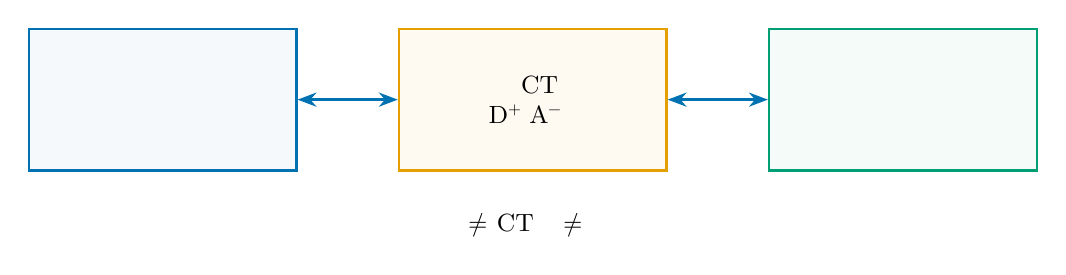
\begin{tikzpicture}[x=1cm,y=1cm,box/.style={draw=tolblue,fill=tolblue!4,line width=.8pt,align=center,inner sep=8pt,font=\small},bi/.style={<->,>=Stealth,line width=.85pt,draw=tolblue}]

\node[box,minimum width=3.4cm,minimum height=1.8cm] (a) at(0,0) {{\cjkfont 中性激子}\\{\cjkfont 同一局部环境}};
\node[box,draw=tolorange,fill=tolorange!5,minimum width=3.4cm,minimum height=1.8cm] (b) at(4.7,0) {{\cjkfont 界面}CT\\D$^{+}${\cjkfont 与}A$^{-}${\cjkfont 关联}};
\node[box,draw=tolgreen,fill=tolgreen!4,minimum width=3.4cm,minimum height=1.8cm] (c) at(9.4,0) {{\cjkfont 可输运载流子}\\{\cjkfont 分离与收集}};
\draw[bi] (a)--(b);\draw[bi] (b)--(c);
\node[font=\small] at(4.7,-1.6) {{\cjkfont 光学激发能} $\ne$ CT{\cjkfont 自由能} $\ne$ {\cjkfont 自由电荷端点差}};
\end{tikzpicture}}
\caption{{\cjkfont 原创示意：激子、界面}\allowbreak{}CT\allowbreak{}{\cjkfont 态与分离载流子是不同描述层级；箭头表示候选路径，不宣称存在唯一顺序。}\allowbreak{}}\label{fig:2}
{\footnotesize\color{SourceGray} {\cjkfont 材料口径}\allowbreak{} \cite{R11} \cite{R12}\nobreak{}{\cjkfont ；界面}\allowbreak{}CT\allowbreak{}{\cjkfont 分解}\allowbreak{} \cite{R14}\par}
\end{figure}
\medskip
% ===== FROZEN SECTION 7 =====
\FloatBarrier
\Needspace{110pt}
\section{{\cjkfont 极化子与无序为什么同时重要}\allowbreak{}}\label{sec:7}
% SOURCE 7-paragraph-0 6d30c3cdf315796088db7a20ad4853866d28cfb00fd67bb2b048f9047dd541f4
{\cjkfont 当电荷进入一个分子，邻近电子云和核坐标会重新调整。电荷与这种形变联合组成的准粒子语言称为极化子。电子转移后环境还未调整，与充分松弛后的能量不同；二者的差异构成重组能的物理来源。后面}\allowbreak{}Marcus\allowbreak{}{\cjkfont 理论中的}\allowbreak{}\ensuremath{\lambda}\allowbreak{}{\cjkfont 描述两套核构型之间的重组代价，不能把它直接等同于库仑结合能或陷阱深度。}\allowbreak{}
\par
% SOURCE 7-paragraph-1 54ba4d5bafdb3407461a4b28128818543edb1121fecc5629f6a13e27e2e68e1c
{\cjkfont 无序有多种来源。位点能量的分布描述能量无序；相邻分子间的重叠和距离分布影响电子耦合；晶域之间的连通性影响能否形成长程输运路径。两个具有相近吸收谱的薄膜，也可以拥有不同的迁移率和回跳概率。}\allowbreak{}
\par
% SOURCE 7-paragraph-2 a69192f18f62a0fa3b497f26031cfeb0ab96487da22c22d1dde1a8b2d3fe9120
{\cjkfont “浅陷阱”和“深陷阱”必须相对于明确参考能量而言。带尾的局域态、化学缺陷、界面}\allowbreak{}CT\allowbreak{}{\cjkfont 态和电极附近的电荷积累，不应只因它们让电流变慢就都压缩成同一个}\allowbreak{}Nt\allowbreak{}{\cjkfont 与}\allowbreak{}Et\nobreak{}{\cjkfont 。若一个表征得到光学}\allowbreak{}Urbach\allowbreak{}{\cjkfont 能，而另一个得到阻抗反演的高斯}\allowbreak{}DOS\allowbreak{}{\cjkfont 宽度，它们也不自动是同一个}\allowbreak{}\ensuremath{\sigma}\nobreak{}{\cjkfont 。}\allowbreak{}
\par
% SOURCE 7-paragraph-3 adc034cdeefdeffb1ad60f05d217d89af0a744b91292d54a3cea2db8b6002448
{\cjkfont 有机输运模型常使用跳跃率、占据阻塞和空间网络。由这种模型得到的有效迁移率会依赖温度、密度和电场。反过来，从一条室温}\allowbreak{}SCLC\allowbreak{}{\cjkfont 曲线得到一个}\allowbreak{}\ensuremath{\mu}\nobreak{}{\cjkfont ，通常不足以唯一反推出微观}\allowbreak{}H\nobreak{}{\cjkfont 、}\allowbreak{}\ensuremath{\lambda}\allowbreak{}{\cjkfont 和局域化长度。}\allowbreak{}
\par
\begin{figure}[!htbp]
\centering
\includegraphics[width=.90\linewidth,height=.38\textheight,keepaspectratio]{figures/disorder_network.pdf}
\caption{{\cjkfont 原创示意：能量分布与空间网络是两种不同信息。颜色表示位点能，连线粗细表示候选耦合，不是实际形貌重建。}\allowbreak{}}\label{fig:3}
{\footnotesize\color{SourceGray} {\cjkfont 有机跳跃输运与温度密度场耦合}\allowbreak{} \cite{R5}\nobreak{}{\cjkfont ；微观}\allowbreak{}MA\allowbreak{}{\cjkfont 适用性反例}\allowbreak{} \cite{R6}\par}
\end{figure}
\medskip
% ===== FROZEN SECTION 8 =====
\FloatBarrier
\Needspace{110pt}
\section{{\cjkfont 当前器件信息与原始数据边界}\allowbreak{}}\label{sec:8}
% SOURCE 8-paragraph-0 db88b8a1133c5b720af59174b7a31af274b0b3df31374fb31b12302dc3091c39
{\cjkfont 当前讨论器件的质量比为}\allowbreak{}D:A=\allowbreak{}1:1.2\nobreak{}{\cjkfont ，层叠为}\allowbreak{}ITO/PEDOT:PSS/\allowbreak{}{\cjkfont 活性层}\allowbreak{}/PDINN/Ag\nobreak{}{\cjkfont 。材料名称由用户暂定为}\allowbreak{}D18:L8-BO\nobreak{}{\cjkfont ，活性层厚度约}\allowbreak{}100 nm\nobreak{}{\cjkfont 。这里保留“暂定”和“约”，不把它们扩展为所有原始样品已经完成身份确认。}\allowbreak{}
\par
% SOURCE 8-paragraph-1 47e756312620b1f7e56682adedd4e4e86cc5adfc80e76167102fbf648f8b3ebf
{\cjkfont 质量比不是体积分数，也不是每一相的可用态数。要转成体积比需要密度；要转成可用图密度还需要分子数、相分布、空间配对及共享态约束。类似地，知道}\allowbreak{}PDINN/Ag\allowbreak{}{\cjkfont 并不自动给出目标器件的注入势垒、界面偶极或表面复合速度。}\allowbreak{}
\par
% SOURCE 8-paragraph-2 4864d890c3c15f6e78a77e7640a3d08082a9a44f9bceddcd0950fecfda027636
{\cjkfont 用户观察暗态与光照的上翘电压近乎相同，这是一条值得保留的定性约束，但不意味着两条电流幅值相同，也不能单独区分体产生、接触或电热机制。目前没有可用于严格检验的同像素暗亮配对，不能从模型中开关}\allowbreak{}light\allowbreak{}{\cjkfont 变量，反过来制造实验配对。}\allowbreak{}
\par
% SOURCE 8-paragraph-3 a0c6381353b8f92a1245f388bceee0455c5ac4d94d9ceb0141f40ed32c2e4c5c
{\cjkfont 原样品}\allowbreak{}3\allowbreak{}{\cjkfont 曾被解释为比样品}\allowbreak{}1\allowbreak{}{\cjkfont 和}\allowbreak{}2\allowbreak{}{\cjkfont 提前约}\allowbreak{}2 V\nobreak{}{\cjkfont 。该解释受到电压列口径差异的实质挑战：源回读与设置电压不能混用，电流峰也不是最早上翘点。完整原始协议、时间序列与实际端压还需对应，因此本书不把“提前}\allowbreak{}2 V\nobreak{}{\cjkfont ”用作拟合目标或机制证据。}\allowbreak{}
\par
\begin{figure}[!htbp]
\centering
\resizebox{.90\linewidth}{!}{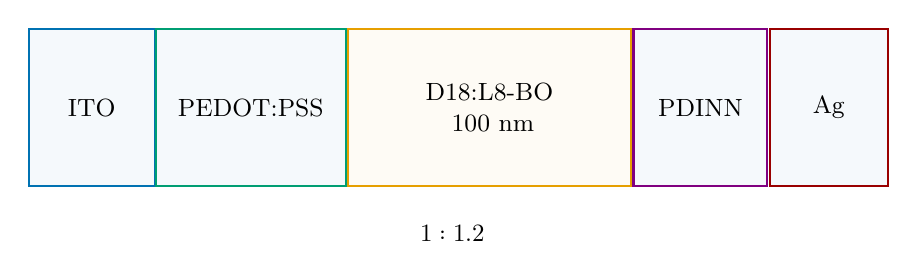
\begin{tikzpicture}[x=1cm,y=1cm,box/.style={draw=tolblue,fill=tolblue!4,line width=.8pt,align=center,inner sep=8pt,font=\small},bi/.style={<->,>=Stealth,line width=.85pt,draw=tolblue}]

\node[box,minimum width=1.6cm,minimum height=2cm] (a) at(0,0) {ITO};
\node[box,draw=tolgreen,minimum width=2.4cm,minimum height=2cm] (b) at(2.02,0) {PEDOT:PSS};
\node[box,draw=tolorange,fill=tolorange!4,minimum width=3.6cm,minimum height=2cm] (c) at(5.05,0) {D18:L8-BO\\{\cjkfont 约}100 nm};
\node[box,draw=violet,minimum width=1.7cm,minimum height=2cm] (d) at(7.73,0) {PDINN};
\node[box,draw=red!60!black,minimum width=1.5cm,minimum height=2cm] (e) at(9.36,0) {Ag};
\node[font=\small] at(4.6,-1.6) {{\cjkfont 给体∶受体质量比} $1:1.2$\quad {\cjkfont 材料身份暂定}};
\end{tikzpicture}}
\caption{{\cjkfont 原创层结构示意。层厚不按比例绘制；仅活性层有约}\allowbreak{}100 nm\allowbreak{}{\cjkfont 的用户估计，其余层厚未知。}\allowbreak{}}\label{fig:4}
{\footnotesize\color{SourceGray} {\cjkfont 样品事实来自本轮用户说明；材料约束记录}\allowbreak{} \cite{D5}\par}
\end{figure}
\medskip
% ===== FROZEN SECTION 9 =====
\FloatBarrier
\Needspace{110pt}
\section{{\cjkfont 上翘}\allowbreak{} \allowbreak{}{\cjkfont 阈值与击穿是三个问题}\allowbreak{}}\label{sec:9}
% SOURCE 9-paragraph-0 a2f347146448a1d533881113f997830081f72b9f8777e4583fa912d65f15bb44
{\cjkfont 反向电流随电压增加而加速增长，可以叫作上翘或膝点，但还需要具体数学定义。一个容易复算的定义是首次达到指定电流密度}\allowbreak{}J*\allowbreak{}{\cjkfont 的电压}\allowbreak{}V*\nobreak{}{\cjkfont 。本项目存档比较使用光照下}\allowbreak{}\ensuremath{\vert}J\ensuremath{\vert}=\allowbreak{}50 mA/cm\textsuperscript{2}\allowbreak{}{\cjkfont 的}\allowbreak{}V50\nobreak{}{\cjkfont ，同时保留}\allowbreak{}V40\allowbreak{}{\cjkfont 与}\allowbreak{}V75\nobreak{}{\cjkfont 。它是比较指标，不是材料损伤的定义。}\allowbreak{}
\par
% SOURCE 9-paragraph-1 21866b8d9e678f7b512cac1cc5889b1e5616f6ba9ed5ea8339ea386f96cf7e18
{\cjkfont 若对不同厚度拟合}\allowbreak{}\ensuremath{\vert}V50\ensuremath{\vert}=\allowbreak{}K50d+b\nobreak{}{\cjkfont ，}\allowbreak{}K50\allowbreak{}{\cjkfont 只是指定阈值、厚度区间和模型下的斜率。非零截距、局部场不均匀、接触压降、光吸收和形貌变化都会影响它。即使}\allowbreak{}R\textsuperscript{2}\allowbreak{}{\cjkfont 很高，也不等于发现了一条普适击穿场定律。}\allowbreak{}
\par
% SOURCE 9-paragraph-2 62df9d9569d92b0fb67d19c5a685465efd7826d516e86ae76b6cc57c0e0882ee
{\cjkfont 电热失稳是温度反馈导致某稳态失去稳定性；不可逆击穿则涉及损伤、导电通道、化学变化或结构重排等不可逆过程。恒温、无损伤变量的稳态模型，即使算到安培每平方厘米，也不能直接输出不可逆击穿电压。数值迭代失败同样不是物理失稳证据。}\allowbreak{}
\par
% SOURCE 9-paragraph-3 2fc61e30c998e085e763dd69150040ca0eac7095d225114333ea199e1989002d
{\cjkfont 下面的温度导数式仅适用于固定}\allowbreak{}\ensuremath{\vert}J\ensuremath{\vert}\allowbreak{}{\cjkfont 阈值、可微且}\allowbreak{}\ensuremath{\partial}F ln\ensuremath{\vert}J\ensuremath{\vert}\allowbreak{}{\cjkfont 非零的单一分支。在非单调曲线中，一个阈值可能被穿越多次。必须规定“从零向反偏的第一次”还是别的规则，并保留全部交叉。如果扫描范围内未跨越，应留空；不能把扫描终点、峰位或求解失败电压补成阈值。}\allowbreak{}
\par
\begin{equation}
|J(V_{50})|=50\ \mathrm{mA\,cm^{-2}},\qquad |V_{50}|=K_{50}d+b
\label{eq:2}\end{equation}
\begin{equation}
\frac{dF^*}{dT}=-\frac{\partial_T\ln |J|}{\partial_F\ln |J|}
\label{eq:3}\end{equation}
\begin{figure}[!htbp]
\centering
\includegraphics[width=.90\linewidth,height=.38\textheight,keepaspectratio]{figures/thresholds.pdf}
\caption{{\cjkfont 原创概念曲线：同一曲线上的阈值、最大曲率和电流峰一般不同。曲线仅为定义示意，没有拟合原始实验。}\allowbreak{}}\label{fig:5}
{\footnotesize\color{SourceGray} {\cjkfont 指标协议}\allowbreak{} \cite{D0}\nobreak{}{\cjkfont ；温度阈值隐函数推导}\allowbreak{} \cite{D3}\par}
\end{figure}
\medskip
% ===== FROZEN SECTION 10 =====
\FloatBarrier
\Needspace{110pt}
\section{{\cjkfont 漂移扩散模型在账本中负责什么}\allowbreak{}}\label{sec:10}
% SOURCE 10-paragraph-0 be57404b383a17972ccae6adc5a83dd1ba8fee0bfa828c4d06f6f114d7b17d0f
{\cjkfont 漂移扩散不是某一种微观产生机制，而是把电荷、输运和源项组织起来的器件层描述。这里以}\allowbreak{}x\allowbreak{}{\cjkfont 从空穴选择性一端指向电子选择性一端，}\allowbreak{}E=\allowbreak{}−\ensuremath{\partial}x\ensuremath{\varphi}\nobreak{}{\cjkfont ；}\allowbreak{}Jn\nobreak{}{\cjkfont 、}\allowbreak{}Jp\allowbreak{}{\cjkfont 都定义为沿}\allowbreak{}+x\allowbreak{}{\cjkfont 的常规电流。电子实际运动方向与}\allowbreak{}Jn\allowbreak{}{\cjkfont 相反。}\allowbreak{}
\par
% SOURCE 10-paragraph-1 2fb09fa75a7c461f05e654443eae2981b295251b5ad619346229a43cf012192e
Poisson\allowbreak{}{\cjkfont 方程决定电势与空间电荷之间的关系；两条连续性方程决定电子和空穴是否有未记账的来源或去向。}\allowbreak{}G\allowbreak{}{\cjkfont 是产对源，}\allowbreak{}R\allowbreak{}{\cjkfont 是复合，二者在电子和空穴方程中成对出现。陷阱占据变化还需要与陷阱电荷一起进入}\allowbreak{}Poisson\allowbreak{}{\cjkfont 与连续性，不能只改一个反应速率而保留不匹配的占据公式。}\allowbreak{}
\par
% SOURCE 10-paragraph-2 f3a126e49241a2c18b28b5f038b343e6b1189c86c1aa5bf840cdfeb12c3dd668
{\cjkfont 普通局域模型中，两种载流子在同一位置产生或复合，总电流的空间导数在稳态为零。如果一次非局域事件在两个不同位置增减电荷，它本身还搬运电荷。仅计算漂移扩散电流会出现空间差异；必须把对应非局域跳跃携带的导电电流纳入总电流。这里称“位移”是指电子跳跃的空间位移，不是}\allowbreak{}Maxwell\allowbreak{}{\cjkfont 的}\allowbreak{}\ensuremath{\varepsilon}\ensuremath{\partial}tE\allowbreak{}{\cjkfont 电流。}\allowbreak{}
\par
% SOURCE 10-paragraph-3 b853279c8a534d27c735265e00a6ffdea8392bb3e8a0e5590bd7a22083d0c406
{\cjkfont 接触边界同样属于模型。固定浓度边界、有限交换速度边界和显式电极能谱不是同一种假设。判断电流是否来自注入，应该读取四个接触粒子通量并与体源积分对比，而不是仅凭能带画法或器件层名猜测。}\allowbreak{}
\par
\begin{equation}
\frac{dE}{dx}=\frac{q}{\varepsilon}(p-n+N_{\mathrm{fixed}}+N_t z_t)
\label{eq:4}\end{equation}
\begin{equation}
J_n=q\mu_n nE+qD_n\frac{dn}{dx},\quad J_p=q\mu_p pE-qD_p\frac{dp}{dx}
\label{eq:5}\end{equation}
\begin{equation}
\partial_t n=\frac{1}{q}\partial_xJ_n+G-R,\quad\partial_t p=-\frac{1}{q}\partial_xJ_p+G-R
\label{eq:6}\end{equation}
\begin{figure}[!htbp]
\centering
\resizebox{.90\linewidth}{!}{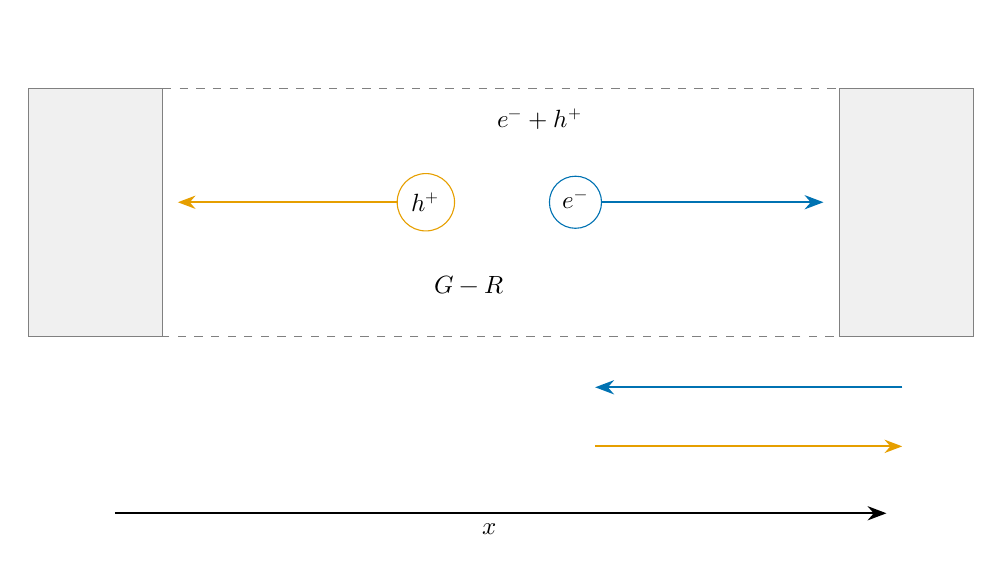
\begin{tikzpicture}[x=1cm,y=1cm,font=\small,
box/.style={draw=tolblue,line width=.75pt,fill=tolblue!3,align=center,inner sep=7pt},
arr/.style={-{Stealth},line width=.85pt,draw=tolblue},
rev/.style={-{Stealth},line width=.75pt,draw=tolorange},
both/.style={<->,>=Stealth,line width=.8pt,draw=tolblue}]

\node[font=\bfseries]at(6,3.8){{\cjkfont 箭头表示粒子运动；先问电子从哪里来}};
\draw[fill=gray!12,draw=gray](0,0)rectangle(1.7,3.15);
\draw[fill=gray!12,draw=gray](10.3,0)rectangle(12,3.15);
\node[align=center]at(.85,1.7){{\cjkfont 左电极}\\{\cjkfont 空穴侧}};
\node[align=center]at(11.15,1.7){{\cjkfont 右电极}\\{\cjkfont 电子侧}};
\draw[dashed,gray](1.7,0)rectangle(10.3,3.15);
\node at(6,2.75){{\cjkfont 活性层：体内成对出现} $e^-+h^+$};
\node[draw=tolorange,circle,inner sep=3pt] (h) at(5.05,1.7){$h^+$};
\node[draw=tolblue,circle,inner sep=3pt] (e) at(6.95,1.7){$e^-$};
\draw[rev](h)--node[above]{{\cjkfont 空穴提取}}(1.9,1.7);
\draw[arr](e)--node[above]{{\cjkfont 电子提取}}(10.1,1.7);
\node at(6,.65){{\cjkfont 体源} $G-R$ {\cjkfont 同时进入两条连续性方程}};
\draw[arr](11.1,-.65)--node[below]{{\cjkfont 电极注入已有电子：边界输入}}(7.2,-.65);
\draw[rev](7.2,-1.4)--node[below]{{\cjkfont 同一边界也允许逆向提取}}(11.1,-1.4);
\draw[arr,black](1.1,-2.25)--node[below]{$x$ {\cjkfont 正向}}(10.9,-2.25);
\node[align=center]at(3.5,-1.10){{\cjkfont 产生与注入不可重复计数}\\{\cjkfont 粒子运动不等于常规电流方向}};
\end{tikzpicture}}
\caption{{\cjkfont 怎样读粒子账本：上半图是假设由体内产对并向两端收集的情形，箭头表示电子或空穴运动，不是常规电流方向。下半图单独画出右接触的电子注入与提取；它们是边界交换，不能再当成新增体产对。实际两类过程可共存，需用四个接触净通量和体源积分区分。电极标签只沿用本书坐标约定，不代表实际选择性已被测定。}\allowbreak{}}\label{fig:6}
{\footnotesize\color{SourceGray} {\cjkfont 方程与实现}\allowbreak{} \cite{D0} \cite{D1}\nobreak{}{\cjkfont ；符号和单位附录}\allowbreak{}\par}
\end{figure}
\medskip
% ===== FROZEN SECTION 11 =====
\FloatBarrier
\Needspace{110pt}
\section{FF78\allowbreak{}{\cjkfont 是共同参照而非样品标定}\allowbreak{}}\label{sec:11}
% SOURCE 11-paragraph-0 dacc65ef52937d799961f28a4c39f9a16007f834e4700f01345cad50496c5122
{\cjkfont 原工程按用户要求构造了接近}\allowbreak{}78\%\allowbreak{}{\cjkfont 的填充因子基准。其接触势垒与平衡迁移率为构造参数；它的意义是让不同候选模型在同一参照上比较，而不是声称所有有机器件都应有这些参数。新增机制后，应报告真正计算出的}\allowbreak{}FF\nobreak{}{\cjkfont ，不能再调}\allowbreak{}\ensuremath{\mu}\allowbreak{}{\cjkfont 把每条曲线都拉回}\allowbreak{}78\%\nobreak{}{\cjkfont 。}\allowbreak{}
\par
% SOURCE 11-paragraph-1 efde4c7d7f2ba758adc58ca83b30dc09430da28723cf60d0cfa6366a98d4c2f4
FF\allowbreak{}{\cjkfont 定义为最大输出功率除以}\allowbreak{}VocJsc\nobreak{}{\cjkfont 。在标准光伏曲线中它描述矩形程度。若某模型因强场复合产生反常}\allowbreak{}J–V\nobreak{}{\cjkfont ，使这个代数比值超过}\allowbreak{}1\nobreak{}{\cjkfont ，不能称为高于}\allowbreak{}100\%\allowbreak{}{\cjkfont 的优质}\allowbreak{}FF\allowbreak{}{\cjkfont 或效率；要同时展示曲线形状，给常规指标标注不适用。}\allowbreak{}
\par
% SOURCE 11-paragraph-2 e6dd7ce926aa0c01040dd9d89f78d2172d61410a127e5c0763e6e8a057644fb8
{\cjkfont 能量采用}\allowbreak{}eV\nobreak{}{\cjkfont 、电势采用}\allowbreak{}V\allowbreak{}{\cjkfont 的数值式时，单位电子跨}\allowbreak{}1 V\allowbreak{}{\cjkfont 等于}\allowbreak{}1 eV\nobreak{}{\cjkfont ；}\allowbreak{}SI\allowbreak{}{\cjkfont 量纲式仍需显式}\allowbreak{}q\nobreak{}{\cjkfont 。本基准中}\allowbreak{}Eg\allowbreak{}{\cjkfont 还同时设置本征浓度、}\allowbreak{}Vbi\allowbreak{}{\cjkfont 及对称陷阱深度；}\allowbreak{}Jgen\allowbreak{}{\cjkfont 则独立固定为}\allowbreak{}25 mA/cm\textsuperscript{2}\nobreak{}{\cjkfont ，未由吸收谱重新积分。改}\allowbreak{}Eg\allowbreak{}{\cjkfont 会联动几处电学定义，却不会自动改变光学响应。这种参数绑定适合透明的示例，但用于材料推断前必须拆开。}\allowbreak{}
\par
\begin{equation}
\mathrm{FF}=\frac{P_{\max}}{V_{\mathrm{oc}}|J_{\mathrm{sc}}|},\quad n_i=N_c e^{-E_g/(2k_BT)},\quad qV_{\mathrm{bi}}=E_g-2\Phi_c
\label{eq:7}\end{equation}
\begin{center}\begin{minipage}{\linewidth}\small
\setlength{\TableWidth}{\dimexpr\linewidth-4\tabcolsep\relax}
\begin{tabular}{@{}>{\raggedright\arraybackslash}p{0.300\TableWidth}>{\raggedright\arraybackslash}p{0.320\TableWidth}>{\raggedright\arraybackslash}p{0.380\TableWidth}@{}}
\toprule
\bfseries {\cjkfont 共同量}\allowbreak{} & \bfseries FF78\allowbreak{}{\cjkfont 设置}\allowbreak{} & \bfseries {\cjkfont 证据类别}\allowbreak{}\\\midrule
d \allowbreak{}{\cjkfont 与}\allowbreak{} T & 100 nm\nobreak{}{\cjkfont ；}\allowbreak{}300 K & {\cjkfont 构造参照}\allowbreak{}\\[3pt]
Eg \allowbreak{}{\cjkfont 与}\allowbreak{} \ensuremath{\varepsilon}r & 1.3 eV\nobreak{}{\cjkfont ；}\allowbreak{}3.5 & {\cjkfont 探索假设}\allowbreak{}\\[3pt]
Nc=\allowbreak{}Nv \allowbreak{}{\cjkfont 与}\allowbreak{} Nt & 10\textsuperscript{19}\nobreak{}{\cjkfont ；}\allowbreak{}10\textsuperscript{15} cm\textsuperscript{−3} & {\cjkfont 探索假设}\allowbreak{}\\[3pt]
\ensuremath{\mu}n=\allowbreak{}\ensuremath{\mu}p & 0.00452474 cm\textsuperscript{2}/Vs & {\cjkfont 为目标}\allowbreak{}FF\allowbreak{}{\cjkfont 构造}\allowbreak{}\\[3pt]
{\cjkfont 接触势垒}\allowbreak{} & 0.05 eV & {\cjkfont 构造边界}\allowbreak{}\\[3pt]
c \allowbreak{}{\cjkfont 与}\allowbreak{} \ensuremath{\beta} & 10\textsuperscript{−9}\nobreak{}{\cjkfont ；}\allowbreak{}10\textsuperscript{−11} cm\textsuperscript{3}/s & {\cjkfont 探索速率尺度}\allowbreak{}\\[3pt]
Jgen & 25 mA/cm\textsuperscript{2} & {\cjkfont 规定光生尺度}\allowbreak{}\\[3pt]
\bottomrule\end{tabular}
\par\vspace{6pt}{\footnotesize\color{SourceGray} baseline\_\allowbreak{}ff78.json\allowbreak{}{\cjkfont 及源代码快照}\allowbreak{} \cite{D0}\nobreak{}{\cjkfont ；本基准未被本书改写}\allowbreak{}\par}
\end{minipage}\end{center}
\medskip
% ===== FROZEN SECTION 12 =====
\FloatBarrier
\Needspace{110pt}
\section{{\cjkfont 先看所有模型再逐项拆解}\allowbreak{}}\label{sec:12}
% SOURCE 12-paragraph-0 7fe61357921985bbdab4588e12ea1f9fcf35b20f447b0d93be887bfdaef74cc7
{\cjkfont 下图来自原}\allowbreak{}FF78\allowbreak{}{\cjkfont 存档比较，所有参数为探索设置。不同模型都可以形成相似的反向上翘，已经足以说明“形状像”不是机制鉴定方法。尤其这些模型不是同一级近似：}\allowbreak{}PF\allowbreak{}{\cjkfont 和}\allowbreak{}MA\allowbreak{}{\cjkfont 跳跃接入}\allowbreak{}Poisson–DD\nobreak{}{\cjkfont ；接触与}\allowbreak{}WKB\allowbreak{}{\cjkfont 微结是并联有效支路；电热是集总动态方程；弱区是面积加权；经验支路只描述曲线。}\allowbreak{}
\par
% SOURCE 12-paragraph-1 6b30c5f20f896a9dd36c21501083ed3a177bc63d3cd55707e33187acb266802f
{\cjkfont 原比较中，}\allowbreak{}PF\nobreak{}{\cjkfont 、}\allowbreak{}MA\allowbreak{}{\cjkfont 和弱区示例都给出}\allowbreak{}FF\allowbreak{}{\cjkfont 与}\allowbreak{}K50\allowbreak{}{\cjkfont 的某种同向变化；接触支路较容易移动反向阈值而对}\allowbreak{}FF\allowbreak{}{\cjkfont 影响很小；电热和经验支路在该厚度假设下}\allowbreak{}K50\allowbreak{}{\cjkfont 接近零。这些是“这一套控制实验的模型结果”，并非真实机制得分。它们的参数轴含义不同，不能把三个点的斜率当成物理普遍性。}\allowbreak{}
\par
% SOURCE 12-paragraph-2 74752434d4b92b965f0c09ffa2bcc4509b5abbdc2a1916e7001b2c304c045618
{\cjkfont 后文将反复区分三个判据：数学账本是否正确；数值计算是否可靠；材料是否支持关键假设。前两项通过后才能讨论第三项，但前两项本身并不能替代第三项。当前工作最有价值的进展正是把这三个问题分开。}\allowbreak{}
\par
\begin{figure}[!htbp]
\centering
\begin{tikzpicture}\begin{semilogyaxis}[width=.90\linewidth,height=.36\textheight,xmin=0,xmax=30,ymin=15,ymax=3000,xlabel={{\cjkfont 反偏电压幅值} / V},ylabel={{\cjkfont 光照电流幅值} / $\mathrm{mA\,cm^{-2}}$},axis lines=left,legend style={font=\scriptsize,at={(0.02,.98)},anchor=north west,legend columns=4},label style={font=\small},tick label style={font=\small}]
\addplot[color=tolblue,solid,line width=.9pt,no marks] coordinates {(0,23.999135557498331) (0.25,24.142997557052961) (0.5,24.249177546596545) (0.75,24.33107998526194) (1,24.396227550937585) (1.25,24.449251308094119) (1.5,24.493191034406205) (1.75,24.530138175590835) (2,24.561584641985228) (2.25,24.588625714777276) (2.5,24.612084662924303) (2.75,24.6325926568454) (3,24.650641850128235) (3.25,24.666621683974363) (3.5,24.680844338218495) (3.75,24.693562956692503) (4,24.704984941991075) (4.25,24.715281813006239) (4.5,24.724596620845659) (4.75,24.733049601183154) (5,24.740742533657404) (5.25,24.747762140467788) (5.5,24.754182762181873) (5.75,24.760068483944831) (6,24.765474838507284) (6.25,24.770450181743346) (6.5,24.775036811023572) (6.75,24.779271881774278) (7,24.783188162229951) (7.25,24.786814659269371) (7.5,24.790177139865829) (7.75,24.793298568405124) (8,24.796199474768159) (8.25,24.798898266081451) (8.5,24.801411491861352) (8.75,24.803754070059867) (9,24.805939480907025) (9.25,24.80797993364131) (9.5,24.809886510421958) (9.75,24.81166929112235) (10,24.813337461823988) (10.25,24.81489940960428) (10.5,24.8163628053716) (10.75,24.817734676672305) (11,24.819021471714336) (11.25,24.820229115876778) (11.5,24.821363061809908) (11.75,24.822428333739332) (12,24.823429566870775) (12.25,24.824371042637019) (12.5,24.82525672012164) (12.75,24.82609026410098) (13,24.82687507043816) (13.25,24.827614288737855) (13.5,24.828310842754014) (13.75,24.828967449060421) (14,24.829586633617804) (14.25,24.830170746994643) (14.5,24.830721978080035) (14.75,24.831242366708992) (15,24.831733814946389) (15.25,24.83219809746608) (15.5,24.83263687117045) (15.75,24.833051683710121) (16,24.833443981584011) (16.25,24.83381511728463) (16.5,24.834166356081216) (16.75,24.83449888216013) (17,24.834813804271821) (17.25,24.835112160930926) (17.5,24.835394925313871) (17.75,24.835663009600818) (18,24.8359172691321) (18.25,24.836158506261036) (18.5,24.836387473793486) (18.75,24.836604878287066) (19,24.836811383107687) (19.25,24.837007611202925) (19.5,24.837194147722951) (19.75,24.837371542493806) (20,24.837540312196221) (20.25,24.837700942540312) (20.5,24.83785389020176) (20.75,24.83799958462642) (21,24.838138429787829) (21.25,24.838270805719507) (21.5,24.838397070026019) (21.75,24.83851755929264) (22,24.838632590326696) (22.25,24.838742461415784) (22.5,24.838847453444298) (22.75,24.838947830940842) (23,24.839043843100253) (23.25,24.839135724673703) (23.5,24.8392236968795) (23.75,24.839307968185974) (24,24.839388735088878) (24.25,24.839466182827778) (24.5,24.839540486060066) (24.75,24.839611809475201) (25,24.83968030841028) (25.25,24.83974612937994) (25.5,24.839809410551066) (25.75,24.839870282470827) (26,24.839928868161358) (26.25,24.839985283790536) (26.5,24.840039639013288) (26.75,24.840092037366755) (27,24.840142576607811) (27.25,24.840191349066362) (27.5,24.840238441942674) (27.75,24.840283937621965) (28,24.840327913948869) (28.25,24.840370444472104) (28.5,24.840411598725545) (28.75,24.840451442424982) (29,24.840490037711426) (29.25,24.840527443346957) (29.5,24.840563714905944) (29.75,24.84059890496227) (30,24.840633063257975)};\addlegendentry{{\cjkfont 局域SRH}}
\addplot[color=tolgreen,solid,line width=.9pt,no marks] coordinates {(0,23.998095622702635) (0.25,24.142243732003685) (0.5,24.24860176502218) (0.75,24.330623113694752) (1,24.395854398702003) (1.25,24.448939684567826) (1.5,24.492926402711966) (1.75,24.52991086836423) (2,24.561388370324991) (2.25,24.588456843010682) (2.5,24.611942027088823) (2.75,24.63247783496702) (3,24.650560024396071) (3.25,24.666583281781417) (3.5,24.680867874345662) (3.75,24.693679836828178) (4,24.705247514473033) (4.25,24.715776864509486) (4.5,24.7254682891752) (4.75,24.734538754585092) (5,24.74325498232767) (5.25,24.751981718882661) (5.5,24.760907007039368) (5.75,24.76946660168408) (6,24.777858901946782) (6.25,24.786315269754517) (6.5,24.795064588392723) (6.75,24.804346454557223) (7,24.814420363684683) (7.25,24.825575074302741) (7.5,24.838137027655179) (7.75,24.852481343203603) (8,24.869044717430597) (8.25,24.888334407866481) (8.5,24.910938694649065) (8.75,24.937546486581418) (9,24.968966002151888) (9.25,25.006132064969925) (9.5,25.050115247932034) (9.75,25.102152276093484) (10,25.163693686076183) (10.25,25.236450537046771) (10.5,25.322433890395843) (10.75,25.423993935572181) (11,25.543865755618288) (11.25,25.685224601728052) (11.5,25.851751277587883) (11.75,26.047707903309057) (12,26.278024782540253) (12.25,26.54839946318133) (12.5,26.865409486219789) (12.75,27.236640561129601) (13,27.670832144854948) (13.25,28.178042667899788) (13.5,28.769836974985836) (13.75,29.459498738157535) (14,30.262271058486633) (14.25,31.195628741390937) (14.5,32.279586230957086) (14.75,33.537045574043802) (15,34.994189381573698) (15.25,36.68092422316262) (15.5,38.631380626555206) (15.75,40.884476487989041) (16,43.484551490247981) (16.25,46.482081008314495) (16.5,49.93447891480465) (16.75,53.906999744864848) (17,58.473751865610218) (17.25,63.718834560900049) (17.5,69.737613372978956) (17.75,76.638149556197888) (18,84.542801296544184) (18.25,93.590016110843919) (18.5,103.9363360126947) (18.75,115.75863916584171) (19,129.25664425151288) (19.25,144.65570636279563) (19.5,162.20993601922484) (19.75,182.2056758846953) (20,204.96537274249971) (20.25,230.85188528149143) (20.5,260.27327093488162) (20.75,293.68809699618794) (21,331.61132171017357) (21.25,374.62078853099371) (21.5,423.36436831752656) (21.75,478.56776401296332) (22,541.04294797352327) (22.25,611.69710583077745) (22.5,691.54174678990364) (22.75,781.70113903766696) (23,883.41796057690044) (23.25,998.0504894341417) (23.5,1127.0440980396431) (23.75,1271.8141923470162) (24,1433.2369499591628) (24.25,1608.4151437417797) (24.5,1756.4867034569329) (24.75,1796.060005071178) (25,1804.2472755631377) (25.25,1807.4345621177097) (25.5,1809.1103923351536) (25.75,1810.1412872821202) (26,1810.8391803328332) (26.25,1811.3431000034698) (26.5,1811.7242263943861) (26.75,1812.022735103204) (27,1812.2630060773881) (27.25,1812.4606864233731) (27.5,1812.6262770268274) (27.75,1812.7670866344611) (28,1812.8883587994658) (28.25,1812.9939530665245) (28.5,1813.0867733114628) (28.75,1813.1690463138898) (29,1813.2425082760562) (29.25,1813.3085329120063) (29.5,1813.3682214029661) (29.75,1813.4224668316219) (30,1813.4720011598083)};\addlegendentry{{\cjkfont 有限PF}}
\addplot[color=tolorange,dashed,line width=.9pt,no marks] coordinates {(0,23.884143683030345) (0.25,24.052631561939148) (0.5,24.175569007883965) (0.75,24.269802736323633) (1,24.34452826253241) (1.25,24.405292766763662) (1.5,24.4556820122482) (1.75,24.498134027765847) (2,24.534371791338327) (2.25,24.565650749964799) (2.5,24.592908830654874) (2.75,24.61686146501718) (3,24.638064172847429) (3.25,24.65695496209214) (3.5,24.673883863599531) (3.75,24.689133958429963) (4,24.702936654679721) (4.25,24.715482945620387) (4.5,24.726931833084691) (4.75,24.737416808829746) (5,24.747050754548003) (5.25,24.755929883346788) (5.5,24.764136811673605) (5.75,24.771743072164121) (6,24.77881127260595) (6.25,24.785397046576161) (6.5,24.791550876623692) (6.75,24.797319555282741) (7,24.802748565668658) (7.25,24.807885177228279) (7.5,24.812784641101501) (7.75,24.817496069789939) (8,24.822092362589199) (8.25,24.82670820527872) (8.5,24.831351306043587) (8.75,24.836375366506907) (9,24.841726644995799) (9.25,24.848148431393717) (9.5,24.855292350552311) (9.75,24.865104699074397) (10,24.875613451320973) (10.25,24.890932013667648) (10.5,24.908980041066464) (10.75,24.931263973519734) (11,24.965342996392128) (11.25,24.998133785957371) (11.5,25.043169491961017) (11.75,25.111922276869759) (12,25.174554768366441) (12.25,25.254046648934814) (12.5,25.374345966649955) (12.75,25.517827274965313) (13,25.638610813984364) (13.25,25.815812918660161) (13.5,26.078547541550247) (13.75,26.36841818354771) (14,26.590886196713878) (14.25,26.908731383812384) (14.5,27.369428143112057) (14.75,28.024332512432093) (15,28.47155250497714) (15.25,28.926798422169139) (15.5,29.566645936376432) (15.75,30.470909252874481) (16,31.741045339413741) (16.25,32.88526178867393) (16.5,33.603745277394722) (16.75,34.569172546023381) (17,35.895498676331322) (17.25,37.721138704703023) (17.5,40.225424780975459) (17.75,43.07235715418097) (18,44.292009708423755) (18.25,45.747423473661549) (18.5,47.683029989725689) (18.75,50.273321448045209) (19,53.743423834692265) (19.25,58.386364171979423) (19.5,64.490180653249269) (19.75,68.567657485788132) (20,70.636052950838945) (20.25,73.218870489226973) (20.5,76.563652480277995) (20.75,80.9161195472401) (21,86.586892501280133) (21.25,93.976241836351122) (21.5,103.59204179895137) (21.75,115.96979599345333) (22,126.58702386397749) (22.25,129.91565320878345) (22.5,133.57005671525914) (22.75,138.12215028791789) (23,143.86399189660443) (23.25,151.12856633861588) (23.5,160.32932344646522) (23.75,171.98664571689156) (24,186.75537040197869) (24.25,205.44950863693779) (24.5,229.01004416099573) (24.75,257.07856691605036) (25,268.66362201131574) (25.25,273.5634970724762) (25.5,279.09558747266806) (25.75,285.78648333729728) (26,293.97683000440276) (26.25,304.03841873981082) (26.5,316.41580658515102) (26.75,331.65149528586682) (27,350.41110612899729) (27.25,373.5120420776795) (27.5,401.95611530931615) (27.75,436.96224281729201) (28,479.97377212416814) (28.25,532.42340153533303) (28.5,589.43471393272819) (28.75,606.29069161101802) (29,613.06015100158231) (29.25,620.13396905818149) (29.5,628.31802658614458) (29.75,637.99064671200176) (30,649.50052714097092)};\addlegendentry{{\cjkfont MA跳跃}}
\addplot[color=violet,dashdotted,line width=.9pt,no marks] coordinates {(0,23.999135557498331) (0.25,24.145875996647792) (0.5,24.253990116919979) (0.75,24.338218662231803) (1,24.406181152819673) (1.25,24.462591627052426) (1.5,24.510575089873207) (1.75,24.55231455351527) (2,24.589401658932317) (2.25,24.62304077902057) (2.5,24.654174635879414) (2.75,24.683565163411416) (3,24.711847544791183) (3.25,24.739567506725678) (3.5,24.76720780905671) (3.75,24.795207566746811) (4,24.82397670606812) (4.25,24.853907053944447) (4.5,24.885381061106344) (4.75,24.918778841943809) (5,24.954484006479326) (5.25,24.992888621489882) (5.5,25.03439754380814) (5.75,25.079432304185822) (6,25.128434673534223) (6.25,25.181870012840307) (6.5,25.240230482995536) (6.75,25.304038176003253) (7,25.373848213982139) (7.25,25.450251855557323) (7.5,25.533879641174835) (7.75,25.625404604915861) (8,25.725545575362268) (8.25,25.835070586417231) (8.5,25.954800416167689) (8.75,26.085612270032858) (9,26.228443624221157) (9.25,26.384296244121344) (9.5,26.554240391879336) (9.75,26.739419237258563) (10,26.941053485459893) (10.25,27.160446235828097) (10.5,27.398988085027622) (10.75,27.658162488957139) (11,27.939551397528515) (11.25,28.244841177017314) (11.5,28.575828835106652) (11.75,28.934428563856521) (12,29.322678616739424) (12.25,29.742748536377665) (12.5,30.196946749885466) (12.75,30.687728549527172) (13,31.217704477423492) (13.25,31.78964913296814) (13.5,32.406510422986763) (13.75,33.071419275502159) (14,33.787699837940394) (14.25,34.558880182614367) (14.5,35.388703542314104) (14.75,36.281140100361448) (15,37.240399359795077) (15.25,38.270943118060202) (15.5,39.377499074343469) (15.75,40.56507509730514) (16,41.838974183117251) (16.25,43.204810133682301) (16.5,44.668523987257331) (16.75,46.236401234103539) (17,47.915089851528009) (17.25,49.711619193943946) (17.5,51.633419775087951) (17.75,53.688343980601005) (18,55.884687751321529) (18.25,58.231213278725654) (18.5,60.737172755588091) (18.75,63.412333227011729) (19,66.267002588348575) (19.25,69.31205677841119) (19.5,72.558968218425548) (19.75,76.019835548994877) (20,79.707414719210718) (20.25,83.63515148457212) (20.5,87.817215372009898) (20.75,92.268535172897018) (21,97.004836027217365) (21.25,102.04267816420443) (21.5,107.39949736763074) (21.75,113.0936472362102) (22,119.14444331225604) (22.25,125.57220915474198) (22.5,132.39832443541817) (22.75,139.64527513982071) (23,147.33670595803073) (23.25,155.49747495304831) (23.5,164.1537105981779) (23.75,173.3328712778862) (24,183.06380735038115) (24.25,193.37682587357145) (24.5,204.30375809990869) (24.75,215.87802984941561) (25,228.13473487430565) (25.25,241.11071133256931) (25.5,254.84462149229853) (25.75,269.37703479322175) (26,284.75051439529062) (26.25,301.00970735097928) (26.5,318.2014385407154) (26.75,336.37480851722273) (27,355.58129540922198) (27.25,375.87486104057132) (27.5,397.31206142629588) (27.75,419.95216181288532) (28,443.85725643604343) (28.25,469.09239317525453) (28.5,495.72570329100336) (28.75,523.82853643672627) (29,553.47560114474015) (29.25,584.74511099202255) (29.5,617.71893665916969) (29.75,652.48276410321841) (30,689.12625907270831)};\addlegendentry{{\cjkfont 接触}}
\addplot[color=red!70!black,densely dashed,line width=.9pt,no marks] coordinates {(0,23.981926571575997) (0.25,24.195533132807256) (0.5,24.409721816371054) (0.75,24.573066072616186) (1,24.738214678499464) (1.25,24.880439491670344) (1.5,25.025602249442692) (1.75,25.159792921510032) (2,25.298020653923096) (2.25,25.431755111149144) (2.5,25.570637870622839) (2.75,25.709162770647598) (3,25.854002487820125) (3.25,26.001507522606389) (3.5,26.156592337583088) (3.75,26.316834367745056) (4,26.486066538897553) (4.25,26.662736135254857) (4.5,26.85000659701296) (4.75,27.04698981732006) (5,27.25645320245415) (5.25,27.478061105247235) (5.5,27.714385498240937) (5.75,27.96559535681148) (6,28.234233707600477) (6.25,28.520978422340171) (6.5,28.828503024146681) (6.75,29.158049722070761) (7,29.512598919840322) (7.25,29.894073154046403) (7.5,30.305980625721489) (7.75,30.751123091195712) (8,31.233840971038241) (8.25,31.758139748242534) (8.5,32.329643541432276) (8.75,32.954090786676048) (9,33.639098965466665) (9.25,34.39302255778621) (9.5,35.226651334579955) (9.75,36.152487757105149) (10,37.186567374847648) (10.25,38.348340741745531) (10.5,39.66298137549952) (10.75,41.162361625211375) (11,42.888697410505351) (11.25,44.897946285756845) (11.5,47.267101230951788) (11.741630565299515,49.999999999999964) (11.75,50.104035061771675) (12,53.56592492070979) (12.25,57.890077748960429) (12.5,63.453772879947842) (12.75,70.894334080503057) (13,81.381052820513773) (13.25,97.313427354567864) (13.5,124.50513920871001) (13.75,181.48734324820475) (14,373.49740845907348) (14.176560982619336,1786.6522276270982)};\addlegendentry{{\cjkfont 电热}}
\addplot[color=gray,dotted,line width=.9pt,no marks] coordinates {(0,23.996716858536058) (0.25,24.266109128419213) (0.5,24.497642067526819) (0.75,24.704814003614889) (1,24.895194651032728) (1.25,25.073446503233804) (1.5,25.242633419149396) (1.75,25.404867777122604) (2,25.561661664984076) (2.25,25.714131307615485) (2.5,25.863122769874472) (2.75,26.009292739669235) (3,26.153162383874093) (3.25,26.295154398855658) (3.5,26.435619221109732) (3.75,26.57485405708179) (4,26.713117047176105) (4.25,26.850638072839619) (4.5,26.987627218104912) (4.75,27.124281578751443) (5,27.260790903674824) (5.25,27.397342414551364) (5.5,27.534125056748824) (5.75,27.671333370936335) (6,27.809171129338182) (6.25,27.947854851069874) (6.5,28.087617287131842) (6.75,28.228710952196391) (7,28.371411766849835) (7.25,28.516022868793371) (7.5,28.662878645317512) (7.75,28.812349037423715) (8,28.964844163131843) (8.25,29.120819308212599) (8.5,29.280780332314084) (8.75,29.445289539365302) (9,29.614972063876991) (9.25,29.790522826583949) (9.5,29.972714115965765) (9.75,30.162403855765184) (10,30.36054462223445) (10.25,30.568193479427137) (10.5,30.786522705184787) (10.75,31.016831486173526) (11,31.260558665593408) (11.25,31.519296633567389) (11.5,31.794806456876969) (11.75,32.089034351527111) (12,32.404129609723498) (12.25,32.742464101063973) (12.5,33.106653476298867) (12.75,33.499580211702089) (13,33.924418642630158) (13.25,34.384662144982045) (13.5,34.884152635556376) (13.75,35.427112574827241) (14,36.018179668150516) (14.25,36.662444476790384) (14.5,37.365491164474527) (14.75,38.133441622014153) (15,38.973003229199549) (15.25,39.89152053236058) (15.5,40.897031135419439) (15.75,41.998326122811164) (16,43.205015356072337) (16.25,44.527598008579751) (16.5,45.977538729484706) (16.75,47.567349854120032) (17,49.310680107449222) (17.25,51.222410277739399) (17.5,53.318756370437654) (17.75,55.617380786631792) (18,58.137512108104382) (18.25,60.900074109877927) (18.5,63.927824663018747) (18.75,67.245505235354642) (19,70.880001744693558) (19.25,74.860517569467632) (19.5,79.218759575304432) (19.75,83.989138072639619) (20,89.208981680591918) (20.25,94.918768136728175) (20.5,101.16237215974914) (20.75,107.98733154455046) (21,115.44513274558869) (21.25,123.59151728538215) (21.5,132.48681041144729) (21.75,142.19627351599675) (22,152.79048192954895) (22.25,164.34572980250479) (22.5,176.94446389717913) (22.75,190.67574822833475) (23,205.63576161237444) (23.25,221.92833031465506) (23.5,239.66549812171061) (23.75,258.96813631006682) (24,279.96659613731958) (24.25,302.80140664370799) (24.5,327.62402072476084) (24.75,354.59761261783342) (25,383.89793013836868) (25.25,415.71420520560906) (25.5,450.25012641348997) (25.75,487.72487763104277) (26,528.37424685683868) (26.25,572.45180980937141) (26.5,620.23019300297619) (26.75,672.00242134538314) (27,728.08335559386921) (27.25,788.81122532566167) (27.5,854.54926341446753) (27.75,925.68744836061069) (28,1002.6443611974165) (28.25,1085.8691640928917) (28.5,1175.8437081843726) (28.75,1273.0847786253046) (29,1378.1464852900187) (29.25,1491.6228080742649) (29.5,1614.1503062486752) (29.75,1746.4110018704664) (30,1889.1354478364353)};\addlegendentry{{\cjkfont 弱区}}
\addplot[color=olive,loosely dashed,line width=.9pt,no marks] coordinates {(0,23.999135557498331) (0.25,24.142997557052961) (0.5,24.249177546596545) (0.75,24.33107998526194) (1,24.396227550937585) (1.25,24.449251308094119) (1.5,24.493191034406205) (1.75,24.530138175590949) (2,24.561584641994582) (2.25,24.588625715072371) (2.5,24.612084667643224) (2.75,24.632592702848463) (3,24.650642159301281) (3.25,24.666623243918636) (3.5,24.680850618654397) (3.75,24.693584057037761) (4,24.705046122455176) (4.25,24.715438900900931) (4.5,24.724961030123932) (4.75,24.733825559834234) (5,24.742278586745734) (5.25,24.750618177276053) (5.5,24.759212840064208) (5.75,24.768518729751765) (6,24.779094817436029) (6.25,24.791615411896739) (6.5,24.806879608913491) (6.75,24.825817454925367) (7,24.849492801061466) (7.25,24.879102988008018) (7.5,24.915975625329271) (7.75,24.961562815640949) (8,25.017433222827293) (8.25,25.085262404443359) (8.5,25.166821823528306) (8.75,25.263966932846046) (9,25.378624691509938) (9.25,25.512780832139363) (9.5,25.668467152251441) (9.75,25.847749058686691) (10,26.052713550157165) (10.25,26.285457782871024) (10.5,26.548078327239622) (10.75,26.842661191983037) (11,27.171272663779249) (11.25,27.535950987406963) (11.5,27.938698891965725) (11.75,28.381476952740648) (12,28.866197766322053) (12.25,29.394720907074181) (12.5,29.968848625759158) (12.75,30.590322246448721) (13,31.260819215120701) (13.25,31.981950750923019) (13.5,32.755260051243432) (13.75,33.582221002232266) (14,34.464237346753087) (14.25,35.402642264599869) (14.5,36.398698321029528) (14.75,37.453597742637861) (15,38.568462981497021) (15.25,39.744347531816196) (15.5,40.982236965771285) (15.75,42.283050157315813) (16,43.647640666391297) (16.25,45.07679825723622) (16.5,46.571250528001421) (16.75,48.131664630263856) (17,49.758649059581565) (17.25,51.452755500112424) (17.5,53.214480708259956) (17.75,55.04426842161557) (18,56.94251128165925) (18.25,58.909552759631033) (18.5,60.945689076308497) (18.75,63.051171108005398) (19,65.226206271816025) (19.25,67.470960384175299) (19.5,69.785559487860326) (19.75,72.170091643229824) (20,74.624608680060163) (20.25,77.149127907410971) (20.5,79.743633778996951) (20.75,82.408079512388312) (21,85.142388660786054) (21.25,87.946456636249565) (21.5,90.820152183982088) (21.75,93.763318807298006) (22,96.775776143172919) (22.25,99.857321288758399) (22.5,103.00773007909602) (22.75,106.22675831666513) (23,109.51414295351394) (23.25,112.86960322669296) (23.5,116.29284174807033) (23.75,119.78354554938953) (24,123.34138708376746) (24.25,126.96602518470721) (24.5,130.6571059838121) (24.75,134.41426378838256) (25,138.23712192017592) (25.25,142.12529351647152) (25.5,146.07838229470681) (25.75,150.0959832822258) (26,154.17768351147734) (26.25,158.32306268308827) (26.5,162.53169379710195) (26.75,166.80314375394497) (27,171.13697392616723) (27.25,175.53274070216139) (27.5,179.98999600289591) (27.75,184.50828777281544) (28,189.08716044589997) (28.25,193.72615538791482) (28.5,198.42481131590893) (28.75,203.18266469579939) (29,207.99925011910514) (29.25,212.87410065963246) (29.5,217.80674821102474) (29.75,222.79672380601548) (30,227.84355791817703)};\addlegendentry{{\cjkfont 经验}}
\addplot[black,dashed,line width=.5pt,forget plot] coordinates {(0,50)(30,50)};\end{semilogyaxis}\end{tikzpicture}
\caption{{\cjkfont 按存档}\allowbreak{}CSV\allowbreak{}{\cjkfont 重绘：}\allowbreak{}100 nm\nobreak{}{\cjkfont 、}\allowbreak{}300 K\nobreak{}{\cjkfont 、各模型默认分支；电热反扫}\allowbreak{}2 V/s\nobreak{}{\cjkfont 。显示}\allowbreak{}15–3000 mA/cm\textsuperscript{2}\nobreak{}{\cjkfont ，完整数据保留；}\allowbreak{}V50\allowbreak{}{\cjkfont 不是损伤阈值。}\allowbreak{}}\label{fig:7}
{\footnotesize\color{SourceGray} {\cjkfont 原候选模型比较与}\allowbreak{}CSV \cite{D0}\par}
\end{figure}
\medskip
% ===== FROZEN SECTION 13 =====
\clearpage
\part*{{\cjkfont 第二部分}\allowbreak{} \allowbreak{}{\cjkfont 完整产生循环}\allowbreak{}}
\FloatBarrier
\Needspace{110pt}
\section{SRH\allowbreak{}{\cjkfont 必须拆成四个物理事件}\allowbreak{}}\label{sec:13}
% SOURCE 13-paragraph-0 4725453953842309ff83faf723b3a269b843a2b8df074d90ee15bd69cd32599e
{\cjkfont 设一个中心空态为}\allowbreak{}0\nobreak{}{\cjkfont ，电子占据态为}\allowbreak{}1\nobreak{}{\cjkfont ，电子占据概率为}\allowbreak{}f\nobreak{}{\cjkfont 。电子捕获把一个已有传导电子放入空中心；电子发射把中心电子释放到传导端点。空穴捕获是中心电子填补价态空穴；空穴发射则是一个原本占据的价态电子进入空中心，留下空穴。第四个过程是暗态持续产生循环中容易被漏掉的“回填”。}\allowbreak{}
\par
% SOURCE 13-paragraph-1 881c959a53eb7169d1996f42ed0ec448bc4f1bbc435be1ef65024b7f9ed2b1ef
{\cjkfont 四个事件必须一起写。把电子发射加速，并不能让刚释放电子的空中心自动再次有电子；若第二次填充来自价态，就必须支付对应跨隙代价；若来自已经存在的传导或接触电子，则它构成运输通道，不能再算一对体产生。}\allowbreak{}
\par
% SOURCE 13-paragraph-2 2f85a444a12eddbf5c8196d312e79becc46aa6abadae232ad051037d146c96e1
cn\nobreak{}{\cjkfont 、}\allowbreak{}cp\allowbreak{}{\cjkfont 是浓度乘子，单位}\allowbreak{}cm\textsuperscript{3}/s\nobreak{}{\cjkfont ；}\allowbreak{}en\nobreak{}{\cjkfont 、}\allowbreak{}ep\allowbreak{}{\cjkfont 是单中心发射率，单位}\allowbreak{}s\textsuperscript{−1}\nobreak{}{\cjkfont 。四个体积事件率都要乘}\allowbreak{}Nt\nobreak{}{\cjkfont ，并包含正确的占据或空位概率。中心电子数的时间变化等于电子捕获加空穴发射，减电子发射与空穴捕获。若}\allowbreak{}f\allowbreak{}{\cjkfont 非常接近}\allowbreak{}1\nobreak{}{\cjkfont ，应单独稳定计算空位概率，而不是用已舍入的}\allowbreak{}1\allowbreak{}{\cjkfont 减}\allowbreak{}f\nobreak{}{\cjkfont 。}\allowbreak{}
\par
\begin{equation}
r_{nc}=N_tc_n n(1-f),\quad r_{ne}=N_te_nf
\label{eq:8}\end{equation}
\begin{equation}
r_{pc}=N_tc_p pf,\quad r_{pe}=N_te_p(1-f)
\label{eq:9}\end{equation}
\begin{equation}
\dot f=(c_n n+e_p)(1-f)-(e_n+c_p p)f
\label{eq:10}\end{equation}
\begin{figure}[!htbp]
\centering
\resizebox{.90\linewidth}{!}{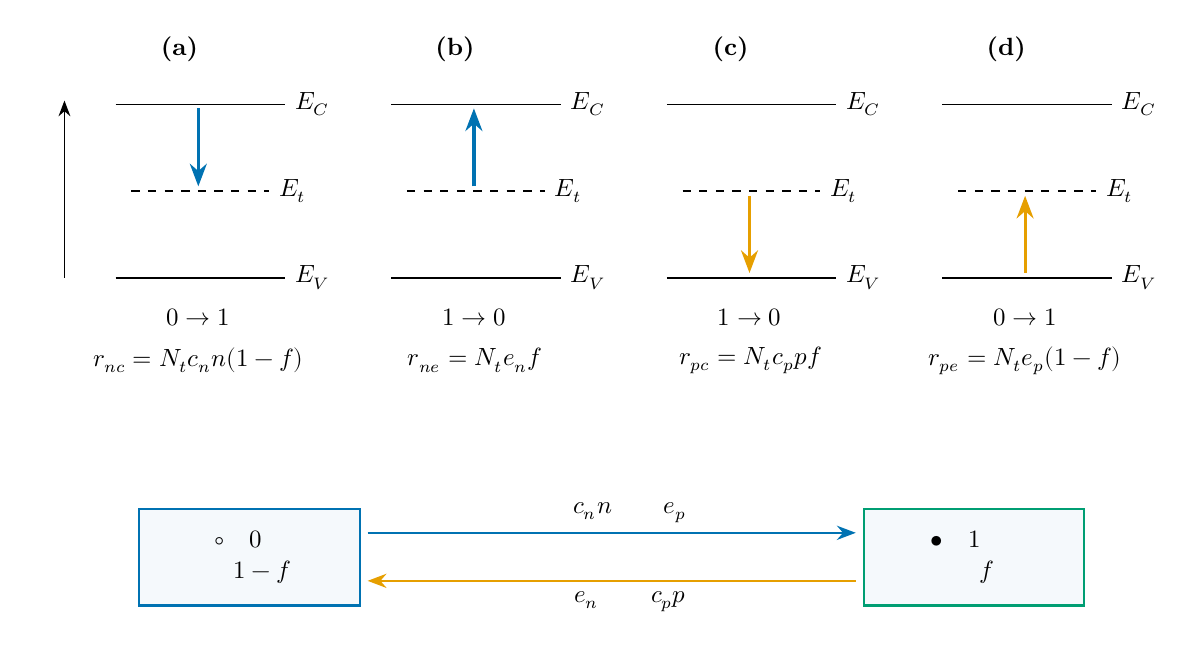
\begin{tikzpicture}[x=1cm,y=1cm,box/.style={draw=tolblue,fill=tolblue!4,line width=.8pt,align=center,inner sep=8pt,font=\small},bi/.style={<->,>=Stealth,line width=.85pt,draw=tolblue}]

% Top panels: every arrow denotes an electron transition, not hole motion.
\foreach \xx/\letter/\title in {0/a/电子捕获,3.5/b/电子发射,7/c/空穴捕获,10.5/d/空穴发射}{
 \begin{scope}[xshift=\xx cm]
  \node[font=\small\bfseries] at(1.05,2.9) {(\letter) {\cjkfont \title}};
  \draw[line width=.65pt] (0,2.2)--(2.15,2.2) node[right,font=\small] {$E_C$};
  \draw[dashed,line width=.65pt] (.2,1.1)--(1.95,1.1) node[right,font=\small] {$E_t$};
  \draw[line width=.65pt] (0,0)--(2.15,0) node[right,font=\small] {$E_V$};
 \end{scope}
}
\draw[-{Stealth},line width=.6pt](-.65,0)--(-.65,2.25);
\node[rotate=90,font=\small]at(-1,1.15){{\cjkfont 电子能量}};
\draw[-{Stealth},tolblue,line width=1.15pt](1.05,2.15)--(1.05,1.16);
\draw[-{Stealth},tolblue,line width=1.15pt](4.55,1.16)--(4.55,2.15);
\draw[-{Stealth},tolorange,line width=1.15pt](8.05,1.04)--(8.05,.06);
\draw[-{Stealth},tolorange,line width=1.15pt](11.55,.06)--(11.55,1.04);
\node[font=\small] at(1.05,-.50) {$0\to1$};
\node[font=\small] at(4.55,-.50) {$1\to0$};
\node[font=\small] at(8.05,-.50) {$1\to0$};
\node[font=\small] at(11.55,-.50) {$0\to1$};
\node[font=\small] at(1.05,-1.05) {$r_{nc}=N_t c_n n(1-f)$};
\node[font=\small] at(4.55,-1.05) {$r_{ne}=N_t e_n f$};
\node[font=\small] at(8.05,-1.05) {$r_{pc}=N_t c_p p f$};
\node[font=\small] at(11.55,-1.05) {$r_{pe}=N_t e_p(1-f)$};
\node[font=\small,align=center] at(1.05,-1.63) {{\cjkfont 移走一个}\ {\cjkfont 传导电子}};
\node[font=\small,align=center] at(4.55,-1.63) {{\cjkfont 增加一个}\ {\cjkfont 传导电子}};
\node[font=\small,align=center] at(8.05,-1.63) {{\cjkfont 填补已有价态空穴}};
\node[font=\small,align=center] at(11.55,-1.63) {{\cjkfont 留下一个价态空穴}};
% Bottom arrows denote the center's occupation changes, not energy or space.
\node[box,minimum width=2.8cm,minimum height=1.15cm] (empty) at(1.7,-3.55) {$\circ\quad 0$ {\cjkfont 空态}\\{\cjkfont 概率} $1-f$};
\node[box,draw=tolgreen,minimum width=2.8cm,minimum height=1.15cm] (filled) at(10.9,-3.55) {$\bullet\quad 1$ {\cjkfont 电子占据}\\{\cjkfont 概率} $f$};
\draw[-{Stealth},line width=.85pt,draw=tolblue] (3.2,-3.24)--node[above,font=\small] {{\cjkfont 电子捕获} $c_n n$ {\cjkfont ＋空穴发射} $e_p$}(9.4,-3.24);
\draw[-{Stealth},line width=.85pt,draw=tolorange] (9.4,-3.85)--node[below,font=\small] {{\cjkfont 电子发射} $e_n$ {\cjkfont ＋空穴捕获} $c_p p$}(3.2,-3.85);
\end{tikzpicture}}
\caption{SRH\allowbreak{}{\cjkfont 四过程能级图及占据循环。上排箭头均表示电子在能级之间的跃迁；}\allowbreak{}Ec\nobreak{}{\cjkfont 、}\allowbreak{}Ev\allowbreak{}{\cjkfont 是传导与价态端点，}\allowbreak{}Et\allowbreak{}{\cjkfont 是中心能级，位置仅为示意。下排}\allowbreak{}0/1\allowbreak{}{\cjkfont 表示中心的电子占据数，不是电荷态；箭头表示占据转变，}\allowbreak{}f\allowbreak{}{\cjkfont 为电子占据概率。各}\allowbreak{}r\allowbreak{}{\cjkfont 是非负的体积事件率，单位}\allowbreak{}cm\textsuperscript{−3} s\textsuperscript{−1}\nobreak{}{\cjkfont ，不能直接相加作为净产生率。空穴捕获由中心电子填补已有空穴；空穴发射由价态电子填入中心并留下空穴。后者不是无需电子与能量的自动复位。}\allowbreak{}}\label{fig:8}
{\footnotesize\color{SourceGray} SRH\allowbreak{}{\cjkfont 原始统计框架}\allowbreak{} \cite{R1}\nobreak{}{\cjkfont ；本项目四速率重构}\allowbreak{} \cite{D0} \cite{D1}\par}
\end{figure}
\medskip
% ===== FROZEN SECTION 14 =====
\FloatBarrier
\Needspace{110pt}
\section{{\cjkfont 从占据方程推到净产生率}\allowbreak{}}\label{sec:14}
% SOURCE 14-paragraph-0 aa7d2491e4a6bfd8be392e73b016479873496eda007f3d9bafd2c239bb4f531f
{\cjkfont 把所有电子端点的捕获率相加为}\allowbreak{}An\nobreak{}{\cjkfont ，空穴端点相加为}\allowbreak{}Ap\nobreak{}{\cjkfont ；电子、空穴发射总率记为}\allowbreak{}En\nobreak{}{\cjkfont 、}\allowbreak{}Ep\nobreak{}{\cjkfont 。它们都具有}\allowbreak{}s\textsuperscript{−1}\allowbreak{}{\cjkfont 单位。稳态占据可直接由两态主方程求出，分母}\allowbreak{}S\allowbreak{}{\cjkfont 是所有离开或进入占据态的总尺度。}\allowbreak{}
\par
% SOURCE 14-paragraph-1 e377638e970070c1fceece51facf49ecedace36e685fbc9139b21dd4eed5d1c2
{\cjkfont 再把}\allowbreak{}f\allowbreak{}{\cjkfont 代回净电子与净空穴反应，就得到相同的每中心净对产生率。分子中的}\allowbreak{}EnEp\allowbreak{}{\cjkfont 代表先形成再发射的完整产生循环，}\allowbreak{}AnAp\allowbreak{}{\cjkfont 代表逆向复合循环。它不是两次发射计数相加；同一对只应计一次。若两个电极之间只发生同种电子捕获再释放，空间电荷会移动，但全器件电子净源为零。}\allowbreak{}
\par
% SOURCE 14-paragraph-2 c40b5739028362e34f7e15777487a92791eba72f8d71f04739bddcec4dc93f76
{\cjkfont 局域热平衡要求}\allowbreak{}np=\allowbreak{}ni\textsuperscript{2}\nobreak{}{\cjkfont ，同时}\allowbreak{}en/cn=\allowbreak{}n1\nobreak{}{\cjkfont 、}\allowbreak{}ep/cp=\allowbreak{}p1\allowbreak{}{\cjkfont 且}\allowbreak{}n1p1=\allowbreak{}ni\textsuperscript{2}\nobreak{}{\cjkfont 。于是产生与复合相抵。注意这不是要求每一种事件都消失：平衡时仍可能有很大的正反周转，只是净流为零。数值上直接从两个极大的量相减，可能把微小净流完全丢失，后面会看到这一点的真实反例。}\allowbreak{}
\par
% SOURCE 14-paragraph-3 1e757a3aac2177b72cd495c5138778344ca3036a443b90350808bba1d2c14dd8
{\cjkfont 这些式子也为模型审查提供捷径：每提出一种场增强，应先检查它怎样改变四个率、占据及正反比，再讨论}\allowbreak{}J–V\allowbreak{}{\cjkfont 是否好看。}\allowbreak{}
\par
\begin{equation}
S=A_n+A_p+E_n+E_p,\quad f=\frac{A_n+E_p}{S},\quad 1-f=\frac{A_p+E_n}{S}
\label{eq:11}\end{equation}
\begin{equation}
R_{\mathrm{pair}}=\frac{E_nE_p-A_nA_p}{S}
\label{eq:12}\end{equation}
\begin{equation}
\frac{e_n}{c_n}=n_1,\quad\frac{e_p}{c_p}=p_1,\quad n_1p_1=n_i^2
\label{eq:13}\end{equation}
\begin{center}\begin{minipage}{\linewidth}\small
\setlength{\TableWidth}{\dimexpr\linewidth-4\tabcolsep\relax}
\begin{tabular}{@{}>{\raggedright\arraybackslash}p{0.300\TableWidth}>{\raggedright\arraybackslash}p{0.320\TableWidth}>{\raggedright\arraybackslash}p{0.380\TableWidth}@{}}
\toprule
\bfseries {\cjkfont 循环}\allowbreak{} & \bfseries {\cjkfont 全器件净源}\allowbreak{} & \bfseries {\cjkfont 可能贡献空间电流}\allowbreak{}\\\midrule
{\cjkfont 价态}\allowbreak{} \ensuremath{\to} \allowbreak{}{\cjkfont 中心}\allowbreak{} \ensuremath{\to} \allowbreak{}{\cjkfont 传导态}\allowbreak{} & {\cjkfont 一对电子空穴}\allowbreak{} & {\cjkfont 是}\allowbreak{}\\[3pt]
{\cjkfont 传导态}\allowbreak{}i \ensuremath{\to} \allowbreak{}{\cjkfont 中心}\allowbreak{} \ensuremath{\to} \allowbreak{}{\cjkfont 传导态}\allowbreak{}j & {\cjkfont 零}\allowbreak{} & {\cjkfont 是}\allowbreak{}\\[3pt]
{\cjkfont 价态空穴}\allowbreak{}i \ensuremath{\leftrightarrow} \allowbreak{}{\cjkfont 中心}\allowbreak{} \ensuremath{\leftrightarrow} \allowbreak{}{\cjkfont 空穴}\allowbreak{}j & {\cjkfont 零}\allowbreak{} & {\cjkfont 是}\allowbreak{}\\[3pt]
{\cjkfont 完整产生的逆过程}\allowbreak{} & {\cjkfont 负一对}\allowbreak{} & {\cjkfont 是}\allowbreak{}\\[3pt]
\bottomrule\end{tabular}
\par\vspace{6pt}{\footnotesize\color{SourceGray} {\cjkfont 独立占据消元与端点循环重构}\allowbreak{} \cite{D1}\par}
\end{minipage}\end{center}
\medskip
% ===== FROZEN SECTION 15 =====
\FloatBarrier
\Needspace{110pt}
\section{{\cjkfont 为什么只把逃逸做快仍然不够}\allowbreak{}}\label{sec:15}
% SOURCE 15-paragraph-0 550330d3c125bf62536dd064099e5d13b4881656a1ebe7ba39c0fb3f522ae5ec
{\cjkfont 在强耗尽、俘获回流可以忽略的理想极限，完整循环率是两个等待时间之和的倒数，即两个发射率标准谐均值的一半，而不是它们的和。直观解释是同一个中心必须等待第一步，再等待第二步。无论第一步怎样加速，第二步仍然限定每秒最多能完成多少个循环。}\allowbreak{}
\par
% SOURCE 15-paragraph-1 884e597b9b2c0394ebfaca2f38ec1b75263d02ea61957d682599f9196decbf7d
{\cjkfont 若对称中带隙的两支起初都是}\allowbreak{}e0\nobreak{}{\cjkfont ，只把一支乘}\allowbreak{}g\nobreak{}{\cjkfont ，则完整循环相对于原}\allowbreak{}e0/2\allowbreak{}{\cjkfont 最多增加两倍。这是一个严格限定的产生上界，不是“一切}\allowbreak{}PF\allowbreak{}{\cjkfont 电流只能翻倍”。接触补给、多中心、额外态或改变另一支的形成物理，都是不同模型，必须重新写循环。}\allowbreak{}
\par
% SOURCE 15-paragraph-2 9111dcfac096e2b4847736aed3117afb02f4f960823e5e6c1ae3b3ccc98fbd2e
FF78\allowbreak{}{\cjkfont 的}\allowbreak{}e0=\allowbreak{}cNc exp[−Eg/(2kBT)]\allowbreak{}{\cjkfont 在}\allowbreak{}300 K\allowbreak{}{\cjkfont 约}\allowbreak{}0.12036 s\textsuperscript{−1}\nobreak{}{\cjkfont 。即使另一支无限快，以}\allowbreak{}Nt=\allowbreak{}10\textsuperscript{15} cm\textsuperscript{−3}\nobreak{}{\cjkfont 、}\allowbreak{}d=\allowbreak{}100 nm\nobreak{}{\cjkfont 、完全收集换算，理想源电流也只有}\allowbreak{}1.928\ensuremath{\times}10\textsuperscript{−10} A/cm\textsuperscript{2}\nobreak{}{\cjkfont ；}\allowbreak{}80 K\allowbreak{}{\cjkfont 降为}\allowbreak{}1.805\ensuremath{\times}10\textsuperscript{−40} A/cm\textsuperscript{2}\nobreak{}{\cjkfont 。这个极小数只约束指定的纯热补给基准。}\allowbreak{}
\par
% SOURCE 15-paragraph-3 d9b490af5704cbcc211e6e5cf9642111dcee79fbefb44ca67c3586ae6fb2fe23
{\cjkfont 这些结果解释了为何“电子很容易逃逸”与“器件有很大持续暗电流”之间仍隔着一个问题。仅初始陷阱放空可以给瞬态电荷，却没有稳态供给；补给来自哪里必须在模型中明确。}\allowbreak{}
\par
\begin{equation}
R=\frac{E_nE_p}{E_n+E_p}=\left(\frac{1}{E_n}+\frac{1}{E_p}\right)^{-1}\leq\min(E_n,E_p)
\label{eq:14}\end{equation}
\begin{equation}
\frac{R(g)}{R(1)}=\frac{2g}{g+1}\leq 2,\qquad J_{\mathrm{cap}}=qN_tdR
\label{eq:15}\end{equation}
\begin{figure}[!htbp]
\centering
\includegraphics[width=.90\linewidth,height=.38\textheight,keepaspectratio]{figures/supply_bottleneck.pdf}
\caption{{\cjkfont 原创解析图：固定慢支路后，快支路增强会饱和。曲线为两态耗尽极限，不是自洽器件}\allowbreak{}J–V\nobreak{}{\cjkfont 。}\allowbreak{}}\label{fig:9}
{\footnotesize\color{SourceGray} {\cjkfont 解析上界与温度重算}\allowbreak{} \cite{D1} \cite{D3}\par}
\end{figure}
\medskip
% ===== FROZEN SECTION 16 =====
\FloatBarrier
\Needspace{110pt}
\section{{\cjkfont 经典}\allowbreak{}PF\allowbreak{}{\cjkfont 降垒从哪一个势函数来}\allowbreak{}}\label{sec:16}
% SOURCE 16-paragraph-0 d706638e1056c0f9eb0e3ba2adc2ed3e0ac8ce91af50f511bc869f3df8e1f11a
Poole–Frenkel\allowbreak{}{\cjkfont 图像考虑载流子从吸引的带电中心附近逃逸。沿有利方向，库仑势随距离上升到零，外场线性倾斜使远处能量下降，两者叠加形成鞍点。对}\allowbreak{}U(r)=\allowbreak{}−A/r−Fr\nobreak{}{\cjkfont ，令导数为零即可得到鞍点位置与降低的势垒。}\allowbreak{}
\par
% SOURCE 16-paragraph-1 3ad9d80f37cdd3d8ba9d0cc12529eebcf1d7da1ab08d16b59a14b86cb226c090
{\cjkfont 这一步有明确前提：有吸引的长程库仑尾势；可以把电荷和介质近似为连续的点电荷体系；鞍点位于核心之外；讨论的是相应方向的逃逸。三维角平均、扩散回捕获、空间电荷和接触供给并未因此自动解决。}\allowbreak{}
\par
% SOURCE 16-paragraph-2 8ae0ff8a2dc5cc0f7cee36e59d784339e55de243f526172c5d3dbf0440b687f6
{\cjkfont 以}\allowbreak{}\ensuremath{\varepsilon}r=\allowbreak{}3.5\nobreak{}{\cjkfont 、}\allowbreak{}2 MV/cm\allowbreak{}{\cjkfont 为例，}\allowbreak{}rs\ensuremath{\approx}\allowbreak{}1.434 nm\nobreak{}{\cjkfont 、降垒}\allowbreak{}\ensuremath{\approx}\allowbreak{}0.574 eV\nobreak{}{\cjkfont 。到}\allowbreak{}3 MV/cm\nobreak{}{\cjkfont ，}\allowbreak{}rs\ensuremath{\approx}\allowbreak{}1.171 nm\nobreak{}{\cjkfont ，已经接近分子长度尺度。这提醒我们检查核心截断、局部屏蔽和电子电荷分布，而不是把根号公式无限外推。}\allowbreak{}
\par
% SOURCE 16-paragraph-3 b8b0d53e8bcaf0101839c09aab363aa4d56d0f199ce68314265cdd36144e14fc
{\cjkfont 经典}\allowbreak{}PF\allowbreak{}{\cjkfont 改变的是某一逃逸路径的势垒。它不能凭名称为两种载流子各赠送一条相同的吸引势，也不能证明每次跨越}\allowbreak{}5 nm\allowbreak{}{\cjkfont 仍具有同样耦合。讨论电流时，还必须回到上一页的完整循环。}\allowbreak{}
\par
\begin{equation}
U(r)=-\frac{A}{r}-Fr,\quad A=\frac{1.43996}{\varepsilon_r}\ \mathrm{eV\,nm}
\label{eq:16}\end{equation}
\begin{equation}
r_s=\sqrt{\frac{A}{F}},\qquad\Delta_{\mathrm{PF}}=2\sqrt{AF}
\label{eq:17}\end{equation}
\begin{figure}[!htbp]
\centering
\includegraphics[width=.90\linewidth,height=.38\textheight,keepaspectratio]{figures/pf_potential.pdf}
\caption{{\cjkfont 原创势函数图：}\allowbreak{}F\allowbreak{}{\cjkfont 用}\allowbreak{}V/nm\nobreak{}{\cjkfont ，}\allowbreak{}\ensuremath{\varepsilon}r=\allowbreak{}3.5\nobreak{}{\cjkfont ；核心附近的虚线区不是连续介质公式的可靠外推区。}\allowbreak{}}\label{fig:10}
{\footnotesize\color{SourceGray} {\cjkfont 吸引库仑中心与}\allowbreak{}PF\allowbreak{}{\cjkfont 逃逸前提}\allowbreak{} \cite{R2}\nobreak{}{\cjkfont ；本报告解析尺度检查}\allowbreak{} \cite{D3} \cite{D5}\par}
\end{figure}
\medskip
% ===== FROZEN SECTION 17 =====
\FloatBarrier
\Needspace{110pt}
\section{{\cjkfont 同一普通两态中心不能任意双支}\allowbreak{}PF}\label{sec:17}
% SOURCE 17-paragraph-0 c4318915b755c1cf1975e0a016f5430f58aa3fe2eb583a78c2ac0cdb1b6393e5
{\cjkfont 设一个普通单电子两态中心的空态电荷为}\allowbreak{}me\nobreak{}{\cjkfont ，占据态为}\allowbreak{}(m−1)e\nobreak{}{\cjkfont 。电子发射后中心处于空态。要让逸出电子受到吸引的单极库仑尾势，残余中心必须为正，因此}\allowbreak{}m\ensuremath{>}0\nobreak{}{\cjkfont 。空穴发射则由价态电子填入中心，最终留下占据态；要吸引被留下的正空穴，这个中心必须为负，因此}\allowbreak{}m−1\ensuremath{<}0\nobreak{}{\cjkfont 。}\allowbreak{}
\par
% SOURCE 17-paragraph-1 fe78cb20804fd0a5bf0de51b97f09fbf7b580ea2bc98d618b69abe7e570993ce
{\cjkfont 两支同时满足上述条件，要求}\allowbreak{}0\ensuremath{<}m\ensuremath{<}1\nobreak{}{\cjkfont 。若}\allowbreak{}m\allowbreak{}{\cjkfont 为普通整数电荷态，这个区间无解。}\allowbreak{}donor\allowbreak{}{\cjkfont 型}\allowbreak{}+/0\allowbreak{}{\cjkfont 中心自然支持电子支的吸引尾势；}\allowbreak{}acceptor\allowbreak{}{\cjkfont 型}\allowbreak{}0/−\allowbreak{}{\cjkfont 中心则自然支持空穴支。把二者都叫作“陷阱”，不能消除电荷态差别。}\allowbreak{}
\par
% SOURCE 17-paragraph-2 cd1fdf7b565f4ee903e9fc34236b48388462ae6dd5692d70fa9978ac462fcc80
{\cjkfont 这个论证的范围应严格限制：它反对的是同一个普通整数电荷、单电子两态中心，两支都使用相同单极}\allowbreak{}PF\allowbreak{}{\cjkfont 吸引势。它没有排除多电荷态、两个缺陷组成的复合体、分布式电荷或显式近态。但后者必须增加相应状态、形成能、占据和返回路径，不能只换一个名称继续使用原率。}\allowbreak{}
\par
% SOURCE 17-paragraph-3 1139154e7829d28cfd96169a2d52504f4e82bd4f02d653ad8b00f943b7f6d887
{\cjkfont 原}\allowbreak{}Poisson\allowbreak{}{\cjkfont 项}\allowbreak{}Nt(0.5−f)\allowbreak{}{\cjkfont 可以表示补偿背景下的电荷约定；它并没有证明一个微观中心真实具有}\allowbreak{}+0.5e\allowbreak{}{\cjkfont 和}\allowbreak{}−0.5e\allowbreak{}{\cjkfont 的两种长程单极尾势。这是平均电荷记账与微观势模型之间的区别。}\allowbreak{}
\par
\begin{equation}
q_{\mathrm{empty}}=me,\quad q_{\mathrm{filled}}=(m-1)e
\label{eq:18}\end{equation}
\begin{equation}
\mathrm{electron\ attraction}:\ m>0,\quad\mathrm{hole\ attraction}:\ m<1
\label{eq:19}\end{equation}
\begin{figure}[!htbp]
\centering
\resizebox{.90\linewidth}{!}{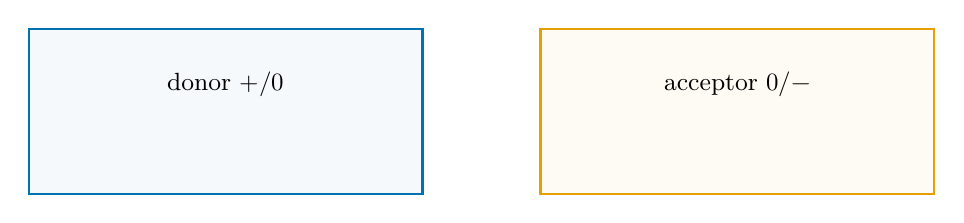
\begin{tikzpicture}[x=1cm,y=1cm,box/.style={draw=tolblue,fill=tolblue!4,line width=.8pt,align=center,inner sep=8pt,font=\small},bi/.style={<->,>=Stealth,line width=.85pt,draw=tolblue}]

\node[box,minimum width=5cm,minimum height=2.1cm] at(0,0) {donor $+/0$\\{\cjkfont 电子发射后残余正核心}\\{\cjkfont 电子吸引尾势}};
\node[box,draw=tolorange,fill=tolorange!4,minimum width=5cm,minimum height=2.1cm] at(6.5,0) {acceptor $0/-$\\{\cjkfont 空穴发射后残余负核心}\\{\cjkfont 空穴吸引尾势}};
\end{tikzpicture}}
\caption{{\cjkfont 原创电荷态示意：}\allowbreak{}donor\allowbreak{}{\cjkfont 的}\allowbreak{}+/0\allowbreak{}{\cjkfont 与}\allowbreak{}acceptor\allowbreak{}{\cjkfont 的}\allowbreak{}0/−\allowbreak{}{\cjkfont 对应不同合法吸引分支。图中不加入未经识别的额外电荷态。}\allowbreak{}}\label{fig:11}
{\footnotesize\color{SourceGray} {\cjkfont 原始}\allowbreak{}PF\allowbreak{}{\cjkfont 电子发射的正残余中心前提}\allowbreak{} \cite{R2}\nobreak{}{\cjkfont ；本次电荷态代数审计}\allowbreak{} \cite{D1}\par}
\end{figure}
\medskip
% ===== FROZEN SECTION 18 =====
\FloatBarrier
\Needspace{110pt}
\section{PF\allowbreak{}{\cjkfont 与}\allowbreak{}Schottky\allowbreak{}{\cjkfont 降垒不能混称}\allowbreak{}}\label{sec:18}
% SOURCE 18-paragraph-0 c36755c6d64e789d8ab1b3b4a4b6dc57b37498a1aa508df33e7e56df07669c08
{\cjkfont 经典}\allowbreak{}PF\allowbreak{}{\cjkfont 考虑体内带电中心的库仑吸引。理想}\allowbreak{}Schottky\allowbreak{}{\cjkfont 图像则考虑载流子靠近金属平面时的像电荷势。像电荷项的系数与孤立单位电荷不同，因此相同介电常数和电场下，理想}\allowbreak{}PF\allowbreak{}{\cjkfont 降垒是理想}\allowbreak{}Schottky\allowbreak{}{\cjkfont 降垒的两倍。下式给降垒的}\allowbreak{}eV\allowbreak{}{\cjkfont 数值；若用焦耳表示势垒，右式整体再乘}\allowbreak{}q\nobreak{}{\cjkfont 。}\allowbreak{}
\par
% SOURCE 18-paragraph-1 3c1f7ddd2f80654c262a4d6844d73d094f11d11138adc8c53e21cc12c26d571c
{\cjkfont 这个二倍关系是两种理想势函数的比较，不是对任何实际有机界面的通用拟合规则。电极表面偶极、界面态、分子取向、无序、隧穿和注入后的空间电荷，都可能改变实际过程。仅在}\allowbreak{}lnJ\allowbreak{}{\cjkfont 对}\allowbreak{}\allowbreak{}\ensuremath{\sqrt{F}}\allowbreak{}{\cjkfont 图上得到一条近似直线，无法唯一鉴定是哪种过程。}\allowbreak{}
\par
% SOURCE 18-paragraph-2 0833dedde683465e72e5ec2f385602d3b9a4fd1a1a5ba64176fdd329050ee239
{\cjkfont 体产生模型需要追踪价态到传导态的完整循环；接触注入模型则从电极储库供给已有电子，后续还要完成电流回路。二者可以产生相似端口曲线，却对电极、厚度、光照和温度的响应不同。若模型只是把一个注入支路并到原}\allowbreak{}DD\allowbreak{}{\cjkfont 上，不能声称已经处理了注入电荷对场的反馈。}\allowbreak{}
\par
% SOURCE 18-paragraph-3 800dc31533a2025037ec0f0eff3b4e3d37198b57118a5a1ba2346ab1ecc7160d
{\cjkfont 本项目后面同时保留}\allowbreak{}PF\allowbreak{}{\cjkfont 启发体源与有效}\allowbreak{}Schottky\allowbreak{}{\cjkfont 支路。它们的共同点是指数率对势垒敏感；不同点是势函数、供给端点以及与器件的耦合层级。把这些差别写清，比给相似曲线贴同一标签更有用。}\allowbreak{}
\par
\begin{equation}
\Delta_{\mathrm{PF}}=\sqrt{\frac{qF}{\pi\varepsilon}},\qquad \Delta_{\mathrm{S}}=\sqrt{\frac{qF}{4\pi\varepsilon}}=\frac{1}{2}\Delta_{\mathrm{PF}}
\label{eq:20}\end{equation}
\begin{center}\begin{minipage}{\linewidth}\small
\setlength{\TableWidth}{\dimexpr\linewidth-4\tabcolsep\relax}
\begin{tabular}{@{}>{\raggedright\arraybackslash}p{0.300\TableWidth}>{\raggedright\arraybackslash}p{0.320\TableWidth}>{\raggedright\arraybackslash}p{0.380\TableWidth}@{}}
\toprule
\bfseries {\cjkfont 问题}\allowbreak{} & \bfseries {\cjkfont 体内}\allowbreak{}PF\allowbreak{}{\cjkfont 逃逸}\allowbreak{} & \bfseries {\cjkfont 理想}\allowbreak{}Schottky\allowbreak{}{\cjkfont 注入}\allowbreak{}\\\midrule
{\cjkfont 势的来源}\allowbreak{} & {\cjkfont 带电中心}\allowbreak{} & {\cjkfont 金属像电荷}\allowbreak{}\\[3pt]
{\cjkfont 供给要追踪什么}\allowbreak{} & {\cjkfont 陷阱形成与复位}\allowbreak{} & {\cjkfont 电极占据与界面交换}\allowbreak{}\\[3pt]
{\cjkfont 电流闭合}\allowbreak{} & {\cjkfont 产生或输运需另判定}\allowbreak{} & {\cjkfont 储库供给及全器件回路}\allowbreak{}\\[3pt]
{\cjkfont 直接套用的风险}\allowbreak{} & {\cjkfont 错设核心电荷态}\allowbreak{} & {\cjkfont 忽略界面及空间电荷}\allowbreak{}\\[3pt]
\bottomrule\end{tabular}
\end{minipage}\end{center}
\begin{figure}[!htbp]
\centering
\resizebox{.90\linewidth}{!}{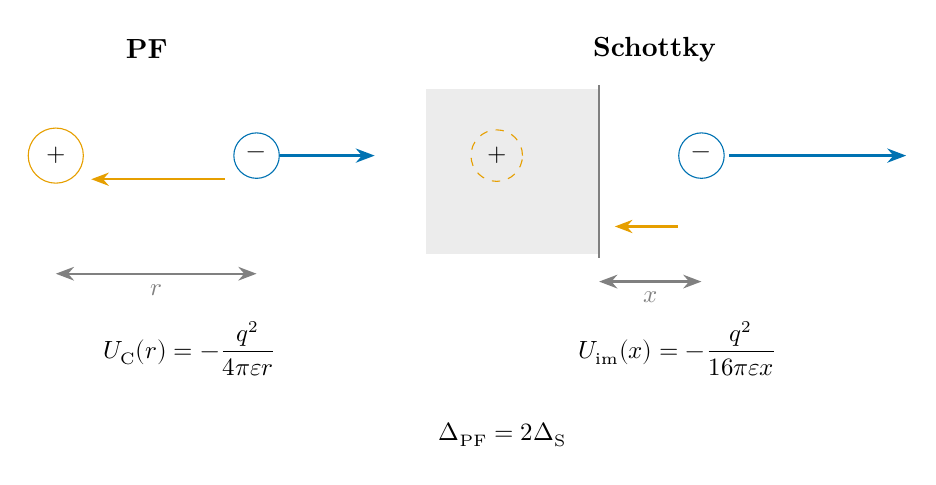
\begin{tikzpicture}[x=1cm,y=1cm,font=\small,
box/.style={draw=tolblue,line width=.75pt,fill=tolblue!3,align=center,inner sep=7pt},
arr/.style={-{Stealth},line width=.85pt,draw=tolblue},
rev/.style={-{Stealth},line width=.75pt,draw=tolorange},
both/.style={<->,>=Stealth,line width=.8pt,draw=tolblue}]

\node[font=\bfseries]at(2.5,3){{\cjkfont 体内PF：真实带电中心}};
\node[font=\bfseries]at(9.0,3){{\cjkfont Schottky：平面像电荷}};
\node[draw=tolorange,circle,minimum size=.70cm]at(1.1,1.65){$+$};
\node[draw=tolblue,circle,minimum size=.52cm]at(3.65,1.65){$-$};
\draw[rev](3.25,1.35)--node[below]{{\cjkfont 库仑吸引}}(1.55,1.35);
\draw[arr](3.95,1.65)--node[above]{{\cjkfont 外场力}}(5.15,1.65);
\draw[both,gray](1.1,.15)--node[below]{$r$}(3.65,.15);
\node at(2.8,-.8){$U_{\rm C}(r)=-\dfrac{q^2}{4\pi\varepsilon r}$};
\fill[gray!15](5.8,.4)rectangle(8.0,2.5);
\draw[gray,line width=1pt](8,.35)--(8,2.55);
\node at(6.7,2.65){{\cjkfont 金属}};
\node[draw=tolorange,dashed,circle,minimum size=.65cm]at(6.7,1.65){$+$};
\node[draw=tolblue,circle,minimum size=.52cm]at(9.3,1.65){$-$};
\node[font=\footnotesize]at(6.7,1.1){{\cjkfont 等效像电荷}};
\draw[rev](9.0,.75)--(8.2,.75);
\node at(9.6,.42){{\cjkfont 像力吸引}};
\draw[arr](9.65,1.65)--node[above]{{\cjkfont 外场力}}(11.9,1.65);
\draw[both,gray](8,.05)--node[below]{$x$}(9.3,.05);
\node at(9.0,-.8){$U_{\rm im}(x)=-\dfrac{q^2}{16\pi\varepsilon x}$};
\node at(6,-1.9){{\cjkfont 相同理想介电常数与场幅值下：}\quad $\Delta_{\rm PF}=2\Delta_{\rm S}$};
\end{tikzpicture}}
\caption{{\cjkfont 两种降垒先从势的来源区分。左图的正中心吸引真实电子；右图用金属平面内的等效正像电荷表示像力，像电荷不是独立供给中心。蓝箭头表示使电子离开的外场力，橙箭头表示吸引力。两条势能式采用}\allowbreak{}SI\allowbreak{}{\cjkfont 单位；像势含金属极化的自能因子，不能直接当作两独立电荷的相互作用能。二倍降垒关系只属于这些理想势及共同介电常数、场幅值，不直接标定真实有机界面。}\allowbreak{}}\label{fig:12}
{\footnotesize\color{SourceGray} PF\allowbreak{}{\cjkfont 前提}\allowbreak{} \cite{R2}\nobreak{}{\cjkfont ；有效接触支路的具体实现}\allowbreak{} \cite{D0}\par}
\end{figure}
\medskip
% ===== FROZEN SECTION 19 =====
\FloatBarrier
\Needspace{110pt}
\section{{\cjkfont 详细平衡约束速率比而非速率大小}\allowbreak{}}\label{sec:19}
% SOURCE 19-paragraph-0 7beac6a8587db4b532f75846ffce5a0289e0ce11d10a42a226553b1981e5b7da
{\cjkfont 给定同一温度下的初态和末态自由能，一条正向跃迁与逆向跃迁的比值受到热力学约束。若电子跨储库交换，还要包括储库电化学势与粒子数变化。}\allowbreak{}\ensuremath{\Delta}N\ensuremath{\alpha}\allowbreak{}{\cjkfont 取从储库}\allowbreak{}\ensuremath{\alpha}\allowbreak{}{\cjkfont 进入所研究系统的粒子数，循环}\allowbreak{}m\allowbreak{}{\cjkfont 取}\allowbreak{}L\ensuremath{\to}R\allowbreak{}{\cjkfont 净转移电子数为正。简并、占据阻塞和场势应进入同一个定义，不能有的藏在}\allowbreak{}\ensuremath{\Delta}G\allowbreak{}{\cjkfont 里，有的又在费米因子里重复计算。}\allowbreak{}
\par
% SOURCE 19-paragraph-1 87299cab1b646d23a8083a28811babf5ac760019126fd9ab8d0612dbfa7e1b2d
{\cjkfont 一个重要但常被混淆的事实是：平衡可以存在静电场。器件内建场由扩散与漂移平衡维持；只要共同电化学势下每条边的正反通量相等，就没有持续净电流。把}\allowbreak{}F\ensuremath{\ne}\allowbreak{}0\allowbreak{}{\cjkfont 直接当成额外泵浦，会在零外偏器件里制造伪暗流。}\allowbreak{}
\par
\begin{center}\begin{minipage}{\linewidth}
\centering
\resizebox{.90\linewidth}{!}{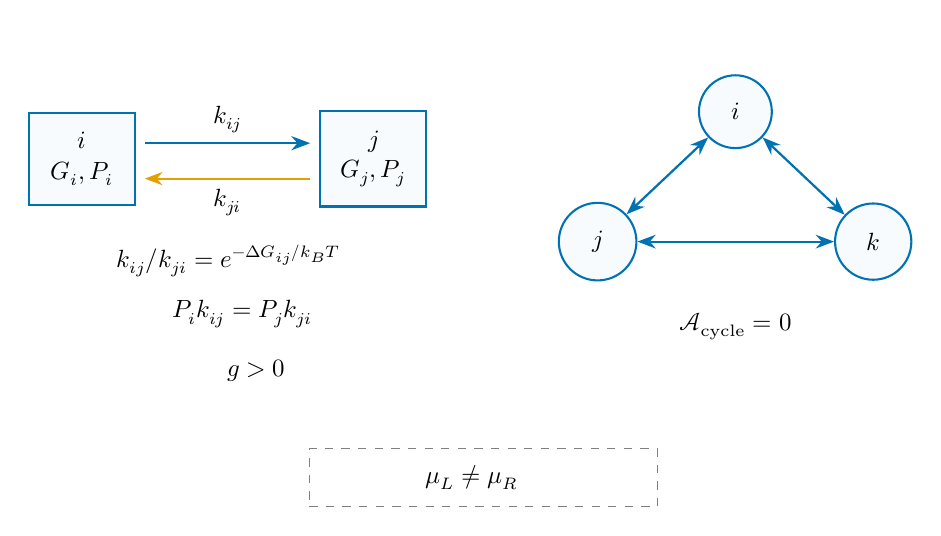
\begin{tikzpicture}[x=1cm,y=1cm,font=\small,
box/.style={draw=tolblue,line width=.75pt,fill=tolblue!3,align=center,inner sep=7pt},
arr/.style={-{Stealth},line width=.85pt,draw=tolblue},
rev/.style={-{Stealth},line width=.75pt,draw=tolorange},
both/.style={<->,>=Stealth,line width=.8pt,draw=tolblue}]

\node[font=\bfseries]at(2.75,3.4){{\cjkfont 一条边：速率与通量分开}};
\node[box,minimum width=1.35cm] (i) at(.9,1.85){$i$\\$G_i,P_i$};
\node[box,minimum width=1.35cm] (j) at(4.6,1.85){$j$\\$G_j,P_j$};
\draw[arr](1.7,2.05)--node[above]{$k_{ij}$}(3.8,2.05);
\draw[rev](3.8,1.60)--node[below]{$k_{ji}$}(1.7,1.60);
\node at(2.75,.55){$k_{ij}/k_{ji}=e^{-\Delta G_{ij}/k_BT}$};
\node at(2.75,-.12){{\cjkfont 平衡：} $P_i k_{ij}=P_j k_{ji}$};
\node[align=center]at(2.75,-1.0){{\cjkfont 两个率共同乘以} $g>0$\\{\cjkfont 比值不变，等待时间改变}};
\node[font=\bfseries]at(9.2,3.4){{\cjkfont 闭合循环：逐边定义一致}};
\node[box,circle,minimum size=.65cm] (a)at(9.2,2.45){$i$};
\node[box,circle,minimum size=.65cm] (b)at(7.45,.8){$j$};
\node[box,circle,minimum size=.65cm] (c)at(10.95,.8){$k$};
\draw[both](a)--(b);\draw[both](b)--(c);\draw[both](c)--(a);
\node[align=center]at(9.2,-.2){{\cjkfont 同温、共同电化学势的平衡}\\$\mathcal A_{\rm cycle}=0$};
\node[align=center]at(9.2,-1.15){{\cjkfont 静电内建场可非零}\\{\cjkfont 仍不能驱动持续净循环}};
\node[draw=gray,dashed,inner sep=6pt]at(6,-2.2){{\cjkfont 持续循环需非平衡驱动，例如}\ $\mu_L\ne\mu_R$\quad {\cjkfont 驱动力和局部场功不能重复计入}};
\end{tikzpicture}}
\captionof{figure}{{\cjkfont 左图箭头表示允许的跃迁，不表示已有净流；}\allowbreak{}Pi\nobreak{}{\cjkfont 、}\allowbreak{}Pj\allowbreak{}{\cjkfont 为状态概率。详细平衡比较的是概率乘速率的通量，而不是要求两方向速率相等。右图是抽象的可逆状态图，节点不指定材料或电荷态；在同一热浴与共同电化学势下，闭合路径的状态能变化相消。不同储库的驱动必须进入同一能量与粒子定义，不能把非零静电场本身当成另一台泵。}\allowbreak{}}\label{fig:13}
{\footnotesize\color{SourceGray} {\cjkfont 有限场逐边平衡}\allowbreak{} \cite{D1}\nobreak{}{\cjkfont ；五个独立循环亲和力验证}\allowbreak{} \cite{D4}\par}
\end{minipage}\end{center}
% SOURCE 19-paragraph-2 9bcc63a871618789315b18d5844d22aded6bb0f86c0b7949dd72ed0d12b6c9ef
{\cjkfont 同时满足详细平衡的率有无穷多组。把一对正反率共同乘以任意正数，不改变比值，却会改变动力学；因此“正反比正确”并不证明某个}\allowbreak{}10\textsuperscript{12} s\textsuperscript{−1}\allowbreak{}{\cjkfont 前因子、某个}\allowbreak{}5 nm\allowbreak{}{\cjkfont 耦合或某个常数储库交换是真实的。后面的量子储库例子正好展示了这种区别。}\allowbreak{}
\par
% SOURCE 19-paragraph-3 7a02d24076437b12dbad2f172e6c54d67844d524e0c5905a452548dcec4707e1
{\cjkfont 对一个闭合循环，所有状态能差首尾相消。持续净循环必须由不同储库的化学势差、外部泵或另一种非平衡来源驱动。局部场功与已经计入的端点电势差不能重复加算。}\allowbreak{}
\par
\begin{equation}
\Delta G_{ij}=G_j-G_i-\sum_\alpha\mu_\alpha\Delta N_\alpha
\label{eq:21}\end{equation}
\begin{equation}
\frac{k_{ij}}{k_{ji}}=\exp\!\left[-\frac{\Delta G_{ij}}{k_BT}\right]
\label{eq:22}\end{equation}
\begin{equation}
\mathcal{A}_{\mathrm{cycle}}=\sum_{(ij)}\ln\frac{k_{ij}}{k_{ji}}=\frac{m(\mu_L-\mu_R)}{k_BT}
\label{eq:23}\end{equation}
\medskip
% ===== FROZEN SECTION 20 =====
\clearpage
\part*{{\cjkfont 第三部分}\allowbreak{} \allowbreak{}{\cjkfont 已尝试的器件模型}\allowbreak{}}
\FloatBarrier
\Needspace{110pt}
\section{{\cjkfont 局域四速率}\allowbreak{}A\allowbreak{}{\cjkfont 到}\allowbreak{}D\allowbreak{}{\cjkfont 究竟改变了什么}\allowbreak{}}\label{sec:20}
% SOURCE 20-paragraph-0 e7565ec3ccbea7b068be41f077de9a8609754e588dee1fde0949a03b70189bf7
{\cjkfont 最直接的诊断是保持局域态和器件结构，只改变四速率的共同倍率。}\allowbreak{}A\allowbreak{}{\cjkfont 不增强，回到原}\allowbreak{}SRH\nobreak{}{\cjkfont ；}\allowbreak{}B\allowbreak{}{\cjkfont 把电子与空穴两对捕获}\allowbreak{}/\allowbreak{}{\cjkfont 发射都乘}\allowbreak{}g\nobreak{}{\cjkfont ；}\allowbreak{}C\allowbreak{}{\cjkfont 只把电子捕获和电子发射这一对乘}\allowbreak{}g\nobreak{}{\cjkfont ；}\allowbreak{}D\allowbreak{}{\cjkfont 只把空穴的一对乘}\allowbreak{}g\nobreak{}{\cjkfont 。因为每一对正反率同步改变，局域平衡能级不变。}\allowbreak{}
\par
% SOURCE 20-paragraph-1 1ab242aa385a5cb293109c9450f094fcd3b2ce79920f8cdd91593911bf4bf7fb
{\cjkfont 这里的}\allowbreak{}g\allowbreak{}{\cjkfont 具有}\allowbreak{}PF\allowbreak{}{\cjkfont 式根号场依赖，并在势垒接近消失时平滑饱和。但}\allowbreak{}A\allowbreak{}{\cjkfont 到}\allowbreak{}D\allowbreak{}{\cjkfont 首先是速率闭合的数学实验，并不是已经识别缺陷电荷态的微观}\allowbreak{}PF\allowbreak{}{\cjkfont 理论。特别是}\allowbreak{}B\allowbreak{}{\cjkfont 的捕获和复合也被极强增强，不能只把它描述成“发射更容易”。}\allowbreak{}
\par
% SOURCE 20-paragraph-2 243675301f411574913d41a7cbbc5296fc960eb8e1536daffdf03cddfc36bf0e
{\cjkfont 固定局域能级、固定}\allowbreak{}ni\allowbreak{}{\cjkfont 时，若只把}\allowbreak{}en\allowbreak{}{\cjkfont 和}\allowbreak{}ep\allowbreak{}{\cjkfont 都乘}\allowbreak{}g\allowbreak{}{\cjkfont 而不改捕获，将在}\allowbreak{}np=\allowbreak{}ni\textsuperscript{2}\allowbreak{}{\cjkfont 的平衡状态下留下净产生，因为两个发射的乘积多了}\allowbreak{}g\textsuperscript{2}\nobreak{}{\cjkfont 。这个错误说明该具体代入不自洽；它不否定所有耗尽区逃逸近似、显式近态或非局域}\allowbreak{}PF\allowbreak{}{\cjkfont 模型。}\allowbreak{}
\par
% SOURCE 20-paragraph-3 16a7c0b2e9f6b819da370cf9022b8027653e3ec5727a561f99794aaf4ca4cbf5
C\allowbreak{}{\cjkfont 和}\allowbreak{}D\allowbreak{}{\cjkfont 在对称接触、相同电子空穴迁移率下有镜像对称性，因此端口曲线接近；它们内部占据和陷阱电荷却不同。不能从端口重合推断真实器件中电子与空穴分支永远等价。}\allowbreak{}
\par
\begin{center}\begin{minipage}{\linewidth}\small
\setlength{\TableWidth}{\dimexpr\linewidth-6\tabcolsep\relax}
\begin{tabular}{@{}>{\raggedright\arraybackslash}p{0.310\TableWidth}>{\raggedright\arraybackslash}p{0.230\TableWidth}>{\raggedright\arraybackslash}p{0.230\TableWidth}>{\raggedright\arraybackslash}p{0.230\TableWidth}@{}}
\toprule
\bfseries {\cjkfont 组别}\allowbreak{} & \bfseries cn \allowbreak{}{\cjkfont 与}\allowbreak{} en & \bfseries cp \allowbreak{}{\cjkfont 与}\allowbreak{} ep & \bfseries {\cjkfont 平衡口径}\allowbreak{}\\\midrule
A & {\cjkfont 原值}\allowbreak{} & {\cjkfont 原值}\allowbreak{} & {\cjkfont 原}\allowbreak{}SRH\\[3pt]
B & {\cjkfont 共同乘}\allowbreak{}g & {\cjkfont 共同乘}\allowbreak{}g & {\cjkfont 四系数共同增强}\allowbreak{}\\[3pt]
C & {\cjkfont 共同乘}\allowbreak{}g & {\cjkfont 原值}\allowbreak{} & {\cjkfont 电子支诊断}\allowbreak{}\\[3pt]
D & {\cjkfont 原值}\allowbreak{} & {\cjkfont 共同乘}\allowbreak{}g & {\cjkfont 空穴支诊断}\allowbreak{}\\[3pt]
\bottomrule\end{tabular}
\end{minipage}\end{center}
\begin{figure}[!htbp]
\centering
\includegraphics[width=.90\linewidth,height=.38\textheight,keepaspectratio]{figures/abcd.pdf}
\caption{{\cjkfont 按存档}\allowbreak{}CSV\allowbreak{}{\cjkfont 重绘：}\allowbreak{}100 nm\nobreak{}{\cjkfont 、}\allowbreak{}300 K\nobreak{}{\cjkfont 、}\allowbreak{}Nt=\allowbreak{}10\textsuperscript{15} cm\textsuperscript{−3}\nobreak{}{\cjkfont 。左为光伏区、右为反向光照；暗态及全部正向数据仍保留。四组未跨}\allowbreak{}V50\nobreak{}{\cjkfont 。}\allowbreak{}}\label{fig:14}
{\footnotesize\color{SourceGray} {\cjkfont 通用四速率诊断与}\allowbreak{}50\allowbreak{}{\cjkfont 项限定检查}\allowbreak{} \cite{D0}\par}
\end{figure}
\medskip
% ===== FROZEN SECTION 21 =====
\FloatBarrier
\Needspace{110pt}
\section{{\cjkfont 局域全倍率为何让光电流塌缩}\allowbreak{}}\label{sec:21}
% SOURCE 21-paragraph-0 3578622afa33d3d8a4275bd0272be71fae0efb5eb31a0cd9e0c115757bc8813e
B\allowbreak{}{\cjkfont 闭合使局域}\allowbreak{}SRH\allowbreak{}{\cjkfont 净率整体乘}\allowbreak{}g\nobreak{}{\cjkfont 。当反偏场很大时，捕获与复合也很强，光生载流子在到达电极前就更多地消失。接近正向低场时，这种增强减弱，反而可能得到大于短路电流的工作区电流，曲线不再具有标准光伏形状。}\allowbreak{}
\par
% SOURCE 21-paragraph-1 b399052ed4e14ed89149a6aa9034171e5fc24b42aee531cd9351565c5b4caa31
{\cjkfont 在}\allowbreak{}Nt=\allowbreak{}10\textsuperscript{15} cm\textsuperscript{−3}\nobreak{}{\cjkfont 、}\allowbreak{}100 nm\allowbreak{}{\cjkfont 的存档结果中，}\allowbreak{}B\allowbreak{}{\cjkfont 的}\allowbreak{}Jsc\allowbreak{}{\cjkfont 约}\allowbreak{}13.55 mA/cm\textsuperscript{2}\nobreak{}{\cjkfont ，}\allowbreak{}Pmax/(VocJsc)\allowbreak{}{\cjkfont 为}\allowbreak{}102.28\%\nobreak{}{\cjkfont ，但常规}\allowbreak{}FF\allowbreak{}{\cjkfont 被留空。}\allowbreak{}Nt=\allowbreak{}10\textsuperscript{16}\allowbreak{}{\cjkfont 时该代数比值甚至达到}\allowbreak{}146.30\%\nobreak{}{\cjkfont 。这是反常曲线的指标问题，不是能量转换超过}\allowbreak{}100\%\nobreak{}{\cjkfont 。反向到}\allowbreak{}−30 V\nobreak{}{\cjkfont ，光照电流只有约}\allowbreak{}5.46\ensuremath{\times}10\textsuperscript{−4} mA/cm\textsuperscript{2}\nobreak{}{\cjkfont ，远没有原有限距离模型的上翘。}\allowbreak{}
\par
% SOURCE 21-paragraph-2 a11bf01a9ccc97f1dd2273af8b066c934cabacc645ca7eb11e7452fde1e52cba
C/D\allowbreak{}{\cjkfont 只增强一个载流子率对，}\allowbreak{}Jsc\allowbreak{}{\cjkfont 约}\allowbreak{}23.33 mA/cm\textsuperscript{2}\nobreak{}{\cjkfont 、}\allowbreak{}FF\allowbreak{}{\cjkfont 约}\allowbreak{}74.18\%\nobreak{}{\cjkfont ，避免了}\allowbreak{}B\allowbreak{}{\cjkfont 那么强的塌缩，却仍没有跨越}\allowbreak{}V40\nobreak{}{\cjkfont 、}\allowbreak{}V50\allowbreak{}{\cjkfont 或}\allowbreak{}V75\nobreak{}{\cjkfont 。单支耗尽产生受慢支上界限制，光照下还同时存在复合与提取，不能把“两倍上界”硬套到所有端口光电流。}\allowbreak{}
\par
% SOURCE 21-paragraph-3 62865240d7ab8bd4b00e2d9f7c42b2168b72347e45187b00fa6a25573c203f71
{\cjkfont 这轮失败给出的正确结论是：这个固定局域态、共同倍率闭合不能在当前参数下同时解释正常光伏与大反向电流。它没有证明所有局域}\allowbreak{}PF\allowbreak{}{\cjkfont 都失败，也没有证明有限距离}\allowbreak{}PF\allowbreak{}{\cjkfont 就具有正确微观机制。}\allowbreak{}
\par
\begin{figure}[!htbp]
\centering
\includegraphics[width=.90\linewidth,height=.38\textheight,keepaspectratio]{figures/local_pf.pdf}
\caption{{\cjkfont 按存档}\allowbreak{}CSV\allowbreak{}{\cjkfont 重绘：正向仅显示光伏工作区，右为反向光照。局域全倍率是一种四系数闭合，不等于所有经典}\allowbreak{}PF\nobreak{}{\cjkfont ；非标准}\allowbreak{}FF\allowbreak{}{\cjkfont 保留原标注。}\allowbreak{}}\label{fig:15}
{\footnotesize\color{SourceGray} {\cjkfont 局域}\allowbreak{}PF\allowbreak{}{\cjkfont 报告、}\allowbreak{}metrics.csv\allowbreak{}{\cjkfont 与代表网格检查}\allowbreak{} \cite{D0}\par}
\end{figure}
\medskip
% ===== FROZEN SECTION 22 =====
\FloatBarrier
\Needspace{110pt}
\section{{\cjkfont 有限距离}\allowbreak{}PF\allowbreak{}{\cjkfont 模型的完整定义}\allowbreak{}}\label{sec:22}
% SOURCE 22-paragraph-0 7aa8f443398452fbfe0d07a13e16b8657f301cf76bc774d1e2a8a4a517d07770
{\cjkfont 以下复述代码采用能量}\allowbreak{}eV\nobreak{}{\cjkfont 、电势}\allowbreak{}V\allowbreak{}{\cjkfont 的数值约定，电势能项的}\allowbreak{}q\allowbreak{}{\cjkfont 由数值换算隐含；}\allowbreak{}SI\allowbreak{}{\cjkfont 式应显式写}\allowbreak{}q\ensuremath{\Delta}\ensuremath{\varphi}\nobreak{}{\cjkfont 。原有限距离}\allowbreak{}PF\allowbreak{}{\cjkfont 启发模型让中心与两侧相距}\allowbreak{}\ensuremath{\ell}\allowbreak{}{\cjkfont 的端点交换载流子。每侧默认}\allowbreak{}\ensuremath{\ell}=\allowbreak{}5 nm\nobreak{}{\cjkfont ，因此最有利的一对电子与空穴端点可相隔}\allowbreak{}10 nm\nobreak{}{\cjkfont 。端点能量随电势差变化；过渡态必须不低于初末端点，从而生成共享势垒的捕获与发射率。}\allowbreak{}
\par
% SOURCE 22-paragraph-1 23c22290d5ecfffff5aec4c6507d0dc18b2620acd6122790ec8c1b00ed0566b1
{\cjkfont 这套构造可以让每一对正反率满足端点能量详细平衡，并让电子、空穴在不同位置出现。由此带来的非局域位移电流必须另外计入，总电流不再仅是}\allowbreak{}Jn+Jp\nobreak{}{\cjkfont 。它是一个明确的假设模型，不是“把}\allowbreak{}SRH\allowbreak{}{\cjkfont 乘了一个}\allowbreak{}PF\allowbreak{}{\cjkfont 因子”的同义词。}\allowbreak{}
\par
% SOURCE 22-paragraph-2 a45fd8a2a58f3e5d5bb176375eda1740079c10cb9f4ae3ceebe81a53cca0cffe
{\cjkfont 实现边界也须公开：场范数实际为}\allowbreak{}\allowbreak{}\ensuremath{\sqrt{E^2+(1\,\mathrm{V/cm})^2}}\nobreak{}{\cjkfont ；}\allowbreak{}\newline{}smoothmax(a,b)=\allowbreak{}\ensuremath{\tfrac{1}{2}}[a+b+\allowbreak{}\ensuremath{\sqrt{(a-b)^2+w^2}}]\nobreak{}{\cjkfont 。请求}\allowbreak{}\ensuremath{\ell}=\allowbreak{}0\allowbreak{}{\cjkfont 仍被强制成一格；}\allowbreak{}\ensuremath{\ell}\ensuremath{>}d\allowbreak{}{\cjkfont 且}\allowbreak{}\ensuremath{\eta}=\allowbreak{}1\allowbreak{}{\cjkfont 时通道全消失而占据成}\allowbreak{}0/0\nobreak{}{\cjkfont 。这些是已发现的参数域缺口，不改变常用}\allowbreak{}5 nm\allowbreak{}{\cjkfont 代表解的账本结论。}\allowbreak{}
\par
% SOURCE 22-paragraph-3 984c3cc0a08dcb105650869d8db74aa1b545cdb9261d66aaddfb8970763c462a
{\cjkfont 核心风险有两项。第一，电子与空穴都使用相同的}\allowbreak{}PF\allowbreak{}{\cjkfont 基础降垒，而普通单中心双支吸引势尚未成立。第二，裸前因子}\allowbreak{}cNc\ensuremath{\eta}/2\allowbreak{}{\cjkfont 不随}\allowbreak{}5 nm\allowbreak{}{\cjkfont 跨度衰减，因此隐含了很强的空间可达性或耦合。参数}\allowbreak{}\ensuremath{\eta}=\allowbreak{}0.5\allowbreak{}{\cjkfont 还会把捕获尺度分到局域和非局域通道，因此蓝紫曲线的差别不能全部归于长度本身。}\allowbreak{}
\par
% SOURCE 22-paragraph-4 82a8ac02557e10666d0b6a6fffc8e443bcd7801beed7935ff3341b6aa3e1d4f5
{\cjkfont 下面的重算保留原方程以审查它到底做了什么，不先把结果删掉或改成较符合预期的形状。}\allowbreak{}
\par
\begin{equation}
\Delta_n=E_g/2-[\phi_e-\phi_t],\quad\Delta_p=E_g/2+[\phi_h-\phi_t]
\label{eq:24}\end{equation}
\begin{equation}
B_0=s_+(E_g/2-\Delta_{\mathrm{PF}}),\quad B=s_+(B_0,\Delta)
\label{eq:25}\end{equation}
\begin{equation}
e=\nu e^{-B/(k_BT)},\quad c=\frac{\nu}{N_c}e^{-(B-\Delta)/(k_BT)},\quad\frac{e}{c}=N_c e^{-\Delta/(k_BT)}
\label{eq:26}\end{equation}
\begin{figure}[!htbp]
\centering
\resizebox{.90\linewidth}{!}{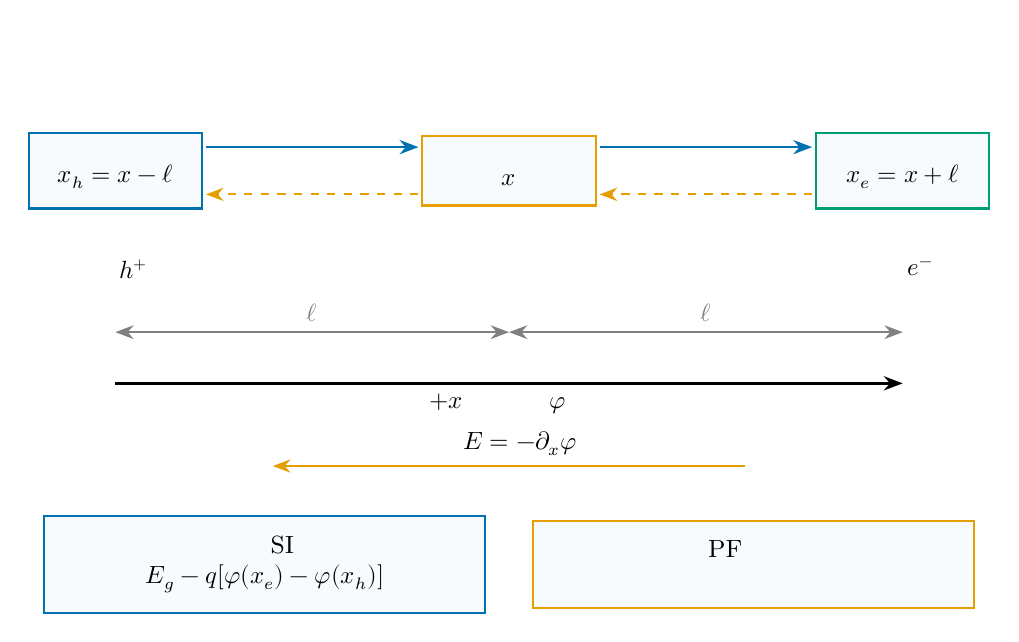
\begin{tikzpicture}[x=1cm,y=1cm,font=\small,
box/.style={draw=tolblue,line width=.75pt,fill=tolblue!3,align=center,inner sep=7pt},
arr/.style={-{Stealth},line width=.85pt,draw=tolblue},
rev/.style={-{Stealth},line width=.75pt,draw=tolorange},
both/.style={<->,>=Stealth,line width=.8pt,draw=tolblue}]

\node[font=\bfseries]at(6,3.8){{\cjkfont 只画最有利的一对端点；实线为电子转移}};
\node[box,minimum width=2.2cm] (v)at(1,2.1){{\cjkfont 价态端点}\\$x_h=x-\ell$};
\node[box,draw=tolorange,minimum width=2.2cm] (t)at(6,2.1){{\cjkfont 中心}\\$x$};
\node[box,draw=tolgreen,minimum width=2.2cm] (c)at(11,2.1){{\cjkfont 传导端点}\\$x_e=x+\ell$};
\draw[arr](2.15,2.4)--node[above]{{\cjkfont 空穴发射}}(4.85,2.4);
\draw[arr](7.15,2.4)--node[above]{{\cjkfont 电子发射}}(9.85,2.4);
\draw[rev,dashed](4.85,1.8)--node[below]{{\cjkfont 空穴捕获}}(2.15,1.8);
\draw[rev,dashed](9.85,1.8)--node[below]{{\cjkfont 电子捕获}}(7.15,1.8);
\node at(1,.85){{\cjkfont 最后留下} $h^+$};
\node at(6,.85){{\cjkfont 中心复位}};
\node at(11,.85){{\cjkfont 最后留下} $e^-$};
\draw[both,gray](1,.05)--node[above]{$\ell$}(6,.05);
\draw[both,gray](6,.05)--node[above]{$\ell$}(11,.05);
\draw[arr,black](1,-.6)--node[below]{$+x$ {\cjkfont 方向；图示有利情形下} $\varphi$ {\cjkfont 升高}}(11,-.6);
\draw[rev](9,-1.65)--node[above]{{\cjkfont 电场}\ $E=-\partial_x\varphi$}(3,-1.65);
\node[box,minimum width=5.6cm]at(2.9,-2.9){{\cjkfont 端点能量差（SI）}\\$E_g-q[\varphi(x_e)-\varphi(x_h)]$};
\node[box,draw=tolorange,minimum width=5.6cm]at(9.1,-2.9){{\cjkfont PF项改变过渡态势垒}\\{\cjkfont 每条边的正反率共享能量定义}};
\end{tikzpicture}}
\caption{{\cjkfont 从左到右读一次完整产对：价态电子进入中心后，中心电子到传导端点，最终在两侧留下同一对空穴和电子。虚线是必须保留的逆过程；图只抽出原模型最有利的非局域端点，未画其它方向和局域通道。图中横轴是真实模型位置而非反应坐标，左向电场有利于电子向右、空穴向左分离。下方把端点电势做功与过渡态降垒分开，场功只计一次；}\allowbreak{}SI\allowbreak{}{\cjkfont 能量式显式含}\allowbreak{}q\nobreak{}{\cjkfont 。距离和电子可达性仍是模型假设，不由示意图证明。}\allowbreak{}}\label{fig:16}
{\footnotesize\color{SourceGray} {\cjkfont 原}\allowbreak{}pf\_\allowbreak{}solver.py\allowbreak{}{\cjkfont 与本次同公式回归}\allowbreak{} \cite{D0} \cite{D1}\par}
\end{figure}
{\small % SOURCE 22-note-0 2b2c185053f9e225792d385d7093d16b65e8d5e9a85840a7f6612e3e1ded4bbf
{\cjkfont 上式}\allowbreak{}s\ensuremath{{}_{+}}\allowbreak{}{\cjkfont 表示代码采用的平滑}\allowbreak{}max\allowbreak{}{\cjkfont 构造；具体双参数}\allowbreak{}smoothmax\allowbreak{}{\cjkfont 和宽度}\allowbreak{}w=\allowbreak{}0.002 eV\allowbreak{}{\cjkfont 见源包。}\allowbreak{}\par}
\medskip
% ===== FROZEN SECTION 23 =====
\FloatBarrier
\Needspace{110pt}
\section{{\cjkfont 只关掉一支降垒电流就消失了吗}\allowbreak{}}\label{sec:23}
% SOURCE 23-paragraph-0 cc6e0a5067d444450c4038a5584916205eb06f954170e5e2fcfdc83ccd6223b8
{\cjkfont 本次重新求解从零偏暗平衡开始，保持}\allowbreak{}FF78\nobreak{}{\cjkfont 、几何、局域通道和对应正反率比不变，只分别关闭电子或空穴支路的}\allowbreak{}PF\allowbreak{}{\cjkfont 降垒。这样避免把“删去补给步骤”误当作“消融}\allowbreak{}PF\nobreak{}{\cjkfont ”。}\allowbreak{}
\par
% SOURCE 23-paragraph-1 13afadf5a968cf0b17d76f7bc7105624b468a8aa8727eaf98d1c3ece379e335e
81\allowbreak{}{\cjkfont 节点、}\allowbreak{}−20 V\allowbreak{}{\cjkfont 暗态，双支}\allowbreak{}PF\allowbreak{}{\cjkfont 为}\allowbreak{}178.8714 mA/cm\textsuperscript{2}\nobreak{}{\cjkfont ；只保留电子支或只保留空穴支时，幅值均约}\allowbreak{}1.3472\ensuremath{\times}10\textsuperscript{−7} mA/cm\textsuperscript{2}\nobreak{}{\cjkfont ；两支都关闭约}\allowbreak{}6.7263\ensuremath{\times}10\textsuperscript{−8} mA/cm\textsuperscript{2}\nobreak{}{\cjkfont 。巨大差异直接证实：当前高电流依赖两条快速支路，单独的快逃逸无法绕过另一支的循环瓶颈。}\allowbreak{}
\par
% SOURCE 23-paragraph-2 a56ac2ec99ac69ebd07b0faec759ee254526abce3fd4c362a7aea63a65c293dd
{\cjkfont 同时，双支结果在}\allowbreak{}161\allowbreak{}{\cjkfont 节点为}\allowbreak{}180.1291\nobreak{}{\cjkfont 、}\allowbreak{}321\allowbreak{}{\cjkfont 节点为}\allowbreak{}180.7502 mA/cm\textsuperscript{2}\nobreak{}{\cjkfont 。后一轮变化}\allowbreak{}0.344\%\nobreak{}{\cjkfont ，因此目前只支持亚百分之一量级的网格稳定性，不能因为端口守恒误差很小就宣称}\allowbreak{}0.1\%\allowbreak{}{\cjkfont 以内精度。缩小电压续接步长的影响更小，主要误差来自空间离散与边界体积。}\allowbreak{}
\par
% SOURCE 23-paragraph-3 ac6003c570cdab70e21462364b0fcd95e0f0ec1a6ed1ccd0e65efd6bb781e96a
{\cjkfont 这不是“证明}\allowbreak{}PF\allowbreak{}{\cjkfont 不可能”。它明确指出旧实现的大电流究竟依赖什么，再要求用真实缺陷电荷态、形成路径和空间耦合来支持或替代这些假设。}\allowbreak{}
\par
\begin{figure}[!htbp]
\centering
\includegraphics[width=.90\linewidth,height=.38\textheight,keepaspectratio]{figures/branch_mesh.pdf}
\caption{2026\allowbreak{}{\cjkfont 年}\allowbreak{}10\allowbreak{}{\cjkfont 月}\allowbreak{}2\allowbreak{}{\cjkfont 日新重算。左为保留正反闭合的分支消融，右为指定双支模型的网格检查。所有值为恒温构造参数下的条件解。}\allowbreak{}}\label{fig:17}
{\footnotesize\color{SourceGray} 45\allowbreak{}{\cjkfont 个新状态、独立率和通量审计}\allowbreak{} \cite{D1}\par}
\end{figure}
\medskip
% ===== FROZEN SECTION 24 =====
\FloatBarrier
\Needspace{110pt}
\section{180 mA\allowbreak{}{\cjkfont 每平方厘米到底从哪里来}\allowbreak{}}\label{sec:24}
% SOURCE 24-paragraph-0 9cedac997380e5acb4c7c9ca598d8886246547eb2e297531c62bd84e6c8112c6
{\cjkfont 对}\allowbreak{}161\allowbreak{}{\cjkfont 节点、}\allowbreak{}−20 V\allowbreak{}{\cjkfont 暗态解，独立按所有价态}\allowbreak{}\ensuremath{\to}\allowbreak{}{\cjkfont 中心}\allowbreak{}\ensuremath{\to}\allowbreak{}{\cjkfont 传导态循环重构的净对源为}\allowbreak{}180.129109 mA/cm\textsuperscript{2}\nobreak{}{\cjkfont ，扣除双分子复合}\allowbreak{}0.000023520 mA/cm\textsuperscript{2}\allowbreak{}{\cjkfont 后，与端口}\allowbreak{}180.129086 mA/cm\textsuperscript{2}\allowbreak{}{\cjkfont 相符。电子与空穴从各自选择性端净输出，反向少数载流子接触流约}\allowbreak{}1.54\ensuremath{\times}10\textsuperscript{−14} mA/cm\textsuperscript{2}\nobreak{}{\cjkfont 。}\allowbreak{}
\par
% SOURCE 24-paragraph-1 5616b6be55974181b785a84f48a645f1a9b4b58a47e9b3ad89ffd32d3cc807d4
{\cjkfont 因此，对这一特定解，把大电流说成主要由电极注入是不正确的。模型确实在体内持续跨隙产生配对载流子，并在电极提取。质疑它应针对产生机制的微观率，而不是把已核实的源误判为漏记的接触供给。}\allowbreak{}
\par
% SOURCE 24-paragraph-2 8460f7383adc78eb21a35e4e3cbd742c1610c5fdcfa4ee39ab2187ba21522032
{\cjkfont 另有同种电子或空穴通过中心搬运的}\allowbreak{}gross\allowbreak{}{\cjkfont 周转，每种等效约}\allowbreak{}0.02717 mA/cm\textsuperscript{2}\nobreak{}{\cjkfont ，但它们的积分粒子源为零，不能再次加到端口产对电流中。独立按每条跳跃跨过哪些网格面组装非局域电流，与原累计源表达式一致。}\allowbreak{}
\par
% SOURCE 24-paragraph-3 a525e83d49b8e8a81815e5ae8d5d4e8da53fba774c3b2a9a48de18fd00e06bab
{\cjkfont 光照}\allowbreak{}−20 V\allowbreak{}{\cjkfont 代表点为约}\allowbreak{}204.9654 mA/cm\textsuperscript{2}\nobreak{}{\cjkfont ，净陷阱对源仍约}\allowbreak{}180.1235 mA/cm\textsuperscript{2}\nobreak{}{\cjkfont 。这个单点说明该参数下高反偏体源对光生浓度不敏感；它没有重新提取暗亮上翘电压，更不能充当实验配对验证。}\allowbreak{}
\par
\begin{figure}[!htbp]
\centering
\includegraphics[width=.90\linewidth,height=.38\textheight,keepaspectratio]{figures/spatial_balance.pdf}
\caption{{\cjkfont 本次重算的空间账本。只有加入非局域位移电流，总电流才能与端口和体源统一。图中局部}\allowbreak{}gross\allowbreak{}{\cjkfont 过程不应被直接相加为净源。}\allowbreak{}}\label{fig:18}
{\footnotesize\color{SourceGray} {\cjkfont 四接触、循环源和跨面位移的独立重构}\allowbreak{} \cite{D1}\par}
\end{figure}
\medskip
% ===== FROZEN SECTION 25 =====
\FloatBarrier
\Needspace{110pt}
\section{{\cjkfont 场功成立不代表已经算出了发热}\allowbreak{}}\label{sec:25}
% SOURCE 25-paragraph-0 138a5a7c56939ce40493de647676a1637fd88a35ae6d589e6d29cdb3ffbe8dbe
{\cjkfont 两步产生的端点能差之和为}\allowbreak{}Eg−[\ensuremath{\varphi}(e)−\ensuremath{\varphi}(h)]\nobreak{}{\cjkfont 。这里电场在电子和空穴分离时做功，恰好由端点电势差体现。}\allowbreak{}PF\allowbreak{}{\cjkfont 项改变过渡态的动力学阻碍；不能再把端点已经计入的场功重复减去一次，以制造额外能量收益。}\allowbreak{}
\par
% SOURCE 25-paragraph-1 ff3df231da3fc6c8fa038834cb561a186f26ba395ce0d6e21799ea3659d9eb0f
−20 V\allowbreak{}{\cjkfont 新解中，净跨隙能量率为}\allowbreak{}0.2341678 W/cm\textsuperscript{2}\nobreak{}{\cjkfont ，产对循环场功}\allowbreak{}0.3818701 W/cm\textsuperscript{2}\nobreak{}{\cjkfont ，二者之差为}\allowbreak{}−0.1477022 W/cm\textsuperscript{2}\nobreak{}{\cjkfont ，表示沿该有利端点方向净下坡。同种输运场功另有}\allowbreak{}0.00007528 W/cm\textsuperscript{2}\nobreak{}{\cjkfont ；全部非局域场功合计}\allowbreak{}0.3819454 W/cm\textsuperscript{2}\nobreak{}{\cjkfont ，与独立积分}\allowbreak{}JnlE\allowbreak{}{\cjkfont 吻合。}\allowbreak{}
\par
% SOURCE 25-paragraph-2 0823f46853fc08213a327be3046f80a8c303a4c5cdaf5ab762ca1e654cde52b5
{\cjkfont 然而端口外电源输入}\allowbreak{}VJ=\allowbreak{}3.6025817 W/cm\textsuperscript{2}\nobreak{}{\cjkfont ，全器件内部}\allowbreak{}\ensuremath{\int}JtotalE dx=\allowbreak{}3.8187366 W/cm\textsuperscript{2}\nobreak{}{\cjkfont ，二者相差}\allowbreak{}−VbiJ\nobreak{}{\cjkfont 。原因是内部静电势差包含内建势，而外加电压只计端口驱动。接触的化学和能量边界项必须一起处理。}\allowbreak{}
\par
% SOURCE 25-paragraph-3 b8083485d75fb22bf8c7bfdfed7d838f0cbc057557654276d2b4d93fcbb63ec8
{\cjkfont 所以这次验证支持一个一致的受驱动能量解释，但没有求解完整接触热流、热浴功率、辐射、热传导或温升。把全部内部场功直接叫作瞬时发热，或由此给出某个温升，都会超出已完成的模型。}\allowbreak{}
\par
\begin{equation}
\Delta_n(e)+\Delta_p(h)=E_g-[\phi(e)-\phi(h)]
\label{eq:27}\end{equation}
\begin{equation}
P_{\mathrm{ext}}=VJ,\qquad\int_0^d J_{\mathrm{tot}}E\,dx=(V-V_{\mathrm{bi}})J
\label{eq:28}\end{equation}
\begin{center}\begin{minipage}{\linewidth}\small
\setlength{\TableWidth}{\dimexpr\linewidth-4\tabcolsep\relax}
\begin{tabular}{@{}>{\raggedright\arraybackslash}p{0.300\TableWidth}>{\raggedright\arraybackslash}p{0.320\TableWidth}>{\raggedright\arraybackslash}p{0.380\TableWidth}@{}}
\toprule
\bfseries {\cjkfont 新解中的能量率}\allowbreak{} & \bfseries W/cm\textsuperscript{2} & \bfseries {\cjkfont 如何解释}\allowbreak{}\\\midrule
{\cjkfont 端口输入}\allowbreak{} & 3.60258 & {\cjkfont 外部电源功率}\allowbreak{}\\[3pt]
{\cjkfont 全部内部电场功}\allowbreak{} & 3.81874 & {\cjkfont 含内建势贡献}\allowbreak{}\\[3pt]
{\cjkfont 非局域事件场功}\allowbreak{} & 0.381945 & {\cjkfont 内部部分位移}\allowbreak{}\\[3pt]
{\cjkfont 两者不能直接相等}\allowbreak{} & {\cjkfont 差}\allowbreak{}0.216155 & {\cjkfont 需接触能量项}\allowbreak{}\\[3pt]
\bottomrule\end{tabular}
\end{minipage}\end{center}
\begin{figure}[!htbp]
\centering
\resizebox{.90\linewidth}{!}{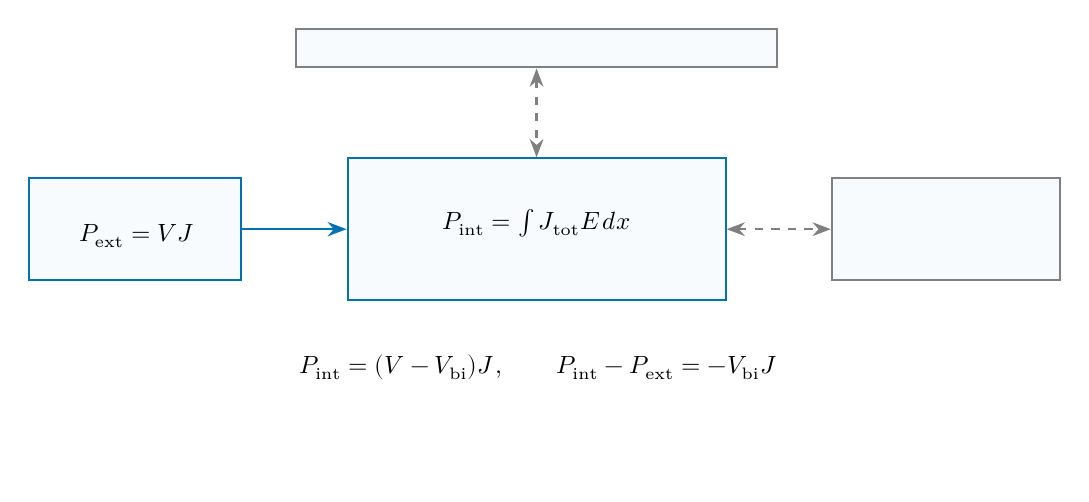
\begin{tikzpicture}[x=1cm,y=1cm,font=\small,
box/.style={draw=tolblue,line width=.75pt,fill=tolblue!3,align=center,inner sep=7pt},
arr/.style={-{Stealth},line width=.85pt,draw=tolblue},
rev/.style={-{Stealth},line width=.75pt,draw=tolorange},
both/.style={<->,>=Stealth,line width=.8pt,draw=tolblue}]

\node[box,minimum width=2.7cm,minimum height=1.3cm](port)at(.9,1.5){{\cjkfont 外部端口}\\$P_{\rm ext}=VJ$};
\node[box,minimum width=4.8cm,minimum height=1.8cm](dev)at(6,1.5){{\cjkfont 器件内部场功}\\$P_{\rm int}=\int J_{\rm tot}E\,dx$\\{\cjkfont 非局域贡献仅是其中一部分}};
\node[box,draw=gray,minimum width=2.9cm,minimum height=1.3cm](bath)at(11.2,1.5){{\cjkfont 热浴与其它能流}\\{\cjkfont 需另行闭合}};
\draw[arr](port)--(dev);
\draw[both,dashed,gray](dev)--(bath);
\node[box,draw=gray,minimum width=6.1cm](contact)at(6,3.8){{\cjkfont 接触的化学与能量边界项}};
\draw[both,dashed,gray](contact)--(dev);
\node at(6,-.25){$P_{\rm int}=(V-V_{\rm bi})J\,,\qquad P_{\rm int}-P_{\rm ext}=-V_{\rm bi}J$};
\node[align=center]at(6,-1.3){{\cjkfont 内建势包含在内部静电势差中}\\{\cjkfont 只有完整能量账本闭合后，才可讨论热流与温升}};
\end{tikzpicture}}
\caption{{\cjkfont 这张图画能量账本的边界，而不是已计算出的热流分配。实线连接外部电功与器件内部描述；虚线提示还需要明确的接触、热浴和其它能流。两行功率关系使用本书电压、电流符号，均为单位面积的功率。内部场功与外部端口功的差不能直接当成热，非局域场功也不是全部器件功率；原模型没有据此求得温升。}\allowbreak{}}\label{fig:19}
{\footnotesize\color{SourceGray} {\cjkfont 端点循环、化学势与电场功独立核验}\allowbreak{} \cite{D1}\par}
\end{figure}
\medskip
% ===== FROZEN SECTION 26 =====
\FloatBarrier
\Needspace{110pt}
\section{{\cjkfont 陷阱密度扫描展示了关联也暴露了假设}\allowbreak{}}\label{sec:26}
% SOURCE 26-paragraph-0 44d41699a403f77f0e58b50293a567fb2a194c8e1fb622283a2efc775660a010
{\cjkfont 原有限距离}\allowbreak{}PF\allowbreak{}{\cjkfont 存档扫描固定}\allowbreak{}\ensuremath{\mu}\nobreak{}{\cjkfont 、接触、捕获系数与长度，只把}\allowbreak{}Nt\allowbreak{}{\cjkfont 从}\allowbreak{}10\textsuperscript{13}\allowbreak{}{\cjkfont 扫到}\allowbreak{}10\textsuperscript{17} cm\textsuperscript{−3}\nobreak{}{\cjkfont 。随着}\allowbreak{}Nt\allowbreak{}{\cjkfont 增大，正向复合与空间电荷增强，}\allowbreak{}FF\allowbreak{}{\cjkfont 下降；反向产生中心增多，指定电流阈值更早达到。这就自然产生了一条}\allowbreak{}FF\allowbreak{}{\cjkfont 与反向阈值的关联，而不必手工规定二者函数关系。}\allowbreak{}
\par
% SOURCE 26-paragraph-1 6ca5b2af565371217754359484352dad9cb6d7163ab538615fa3ab7f8b0757d0
{\cjkfont 例如}\allowbreak{}Nt=\allowbreak{}10\textsuperscript{14}\allowbreak{}{\cjkfont 时}\allowbreak{}FF\allowbreak{}{\cjkfont 约}\allowbreak{}80.18\%\nobreak{}{\cjkfont 、}\allowbreak{}V50\ensuremath{\approx}\allowbreak{}−20.62 V\nobreak{}{\cjkfont ；}\allowbreak{}10\textsuperscript{15}\allowbreak{}{\cjkfont 时}\allowbreak{}77.95\%\nobreak{}{\cjkfont 、}\allowbreak{}−16.50 V\nobreak{}{\cjkfont ；}\allowbreak{}10\textsuperscript{16}\allowbreak{}{\cjkfont 时}\allowbreak{}68.57\%\nobreak{}{\cjkfont 、}\allowbreak{}−12.82 V\nobreak{}{\cjkfont ；}\allowbreak{}10\textsuperscript{17}\allowbreak{}{\cjkfont 时}\allowbreak{}44.61\%\nobreak{}{\cjkfont 、}\allowbreak{}−9.64 V\nobreak{}{\cjkfont 。最低密度点在指定范围没有达到阈值，仍然留空。}\allowbreak{}
\par
% SOURCE 26-paragraph-2 f03171e1dda468f400e43db1d81e519a78e32e4d1db1b4a8a503f6804920684d
{\cjkfont 但是，“同一参数可同时影响正向与反向”只能说明机制在结构上有可能产生关联。由于反向大源仍依赖双支降垒和远距耦合，当前关联不能反过来验证那两项假设，也不能从一条实验}\allowbreak{}FF–K\allowbreak{}{\cjkfont 趋势唯一反推出}\allowbreak{}Nt\nobreak{}{\cjkfont 。}\allowbreak{}
\par
% SOURCE 26-paragraph-3 d486626d3cfc6b8cb09c2338dc9088d6c54c16b79e860d96e7169fe1b216f473
{\cjkfont 另一个隐藏变量是陷阱身份。}\allowbreak{}SCLC\allowbreak{}{\cjkfont 或电容谱得到的浅态密度，未必是反偏跨隙产生所用的深中心密度；两者即使数值接近，也不能互换。必须同时说明密度、能量、电荷态和通道。}\allowbreak{}
\par
\begin{figure}[!htbp]
\centering
\begin{tikzpicture}\begin{groupplot}[group style={group size=2 by 1,horizontal sep=1.3cm},width=.43\linewidth,height=.32\textheight,xmode=log,axis lines=left,label style={font=\small},tick label style={font=\small},xlabel={{\cjkfont 有效} $N_t$ / $\mathrm{cm^{-3}}$}]
\nextgroupplot[ylabel={FF / \%}]
\addplot[tolblue,mark=*,mark size=1.5pt,line width=.8pt] coordinates {(10000000000000,80.460334455557444) (17782794100389.227,80.435710236713049) (31622776601683.793,80.392109230236159) (56234132519034.906,80.315189656718658) (100000000000000,80.180831480505475) (177827941003892.28,79.949427226272675) (316227766016837.94,79.559749553342883) (562341325190349.06,78.926433838514328) (1000000000000000,77.948471334587182) (1778279410038922.8,76.520059753361835) (3162277660168379.5,74.547303470129449) (5623413251903491,71.964449810533921) (10000000000000000,68.567304576377566) (17782794100389228,64.146128920853968) (31622776601683792,58.565426713324499) (56234132519034912,51.911987054939537) (1e+17,44.611061830327337)};
\nextgroupplot[ylabel={$|V_{50}|$ / V}]
\addplot[tolorange,mark=square*,mark size=1.5pt,line width=.8pt] coordinates {(17782794100389.227,24.007947930463843) (31622776601683.793,22.844334515962416) (56234132519034.906,21.72062728250846) (100000000000000,20.620360119502859) (177827941003892.28,19.551001107300841) (316227766016837.94,18.509550056162134) (562341325190349.06,17.493318171227102) (1000000000000000,16.504123394690566) (1778279410038922.8,15.539834420390017) (3162277660168379.5,14.603149028190971) (5623413251903491,13.697804888110348) (10000000000000000,12.818660312587989) (17782794100389228,11.972510694883253) (31622776601683792,11.153885746307923) (56234132519034912,10.375299756216794) (1e+17,9.6441048889492897)};
\end{groupplot}\end{tikzpicture}
\caption{{\cjkfont 存档}\allowbreak{}17\allowbreak{}{\cjkfont 点密度扫描，}\allowbreak{}100 nm\nobreak{}{\cjkfont 、}\allowbreak{}300 K\nobreak{}{\cjkfont 、固定其余}\allowbreak{}FF78\allowbreak{}{\cjkfont 和}\allowbreak{}PF\allowbreak{}{\cjkfont 参数；有效}\allowbreak{}Nt\allowbreak{}{\cjkfont 为探索量，未作样品拟合。}\allowbreak{}}\label{fig:20}
{\footnotesize\color{SourceGray} pf\_\allowbreak{}density\_\allowbreak{}scan\allowbreak{}{\cjkfont 的完整}\allowbreak{}CSV\allowbreak{}{\cjkfont 与代表点网格检查}\allowbreak{} \cite{D0}\par}
\end{figure}
\medskip
% ===== FROZEN SECTION 27 =====
\FloatBarrier
\Needspace{110pt}
\section{{\cjkfont 厚度斜率不是一种机制的指纹}\allowbreak{}}\label{sec:27}
% SOURCE 27-paragraph-0 066605dcb08d5df0afabf44fac13b0dd35b84c7fb1e85c729f856c0c5a305821
{\cjkfont 若一个机制主要由局部场驱动，且其它因素变化较小，随厚度增大达到某场尺度可能需要更大电压，因此}\allowbreak{}Vth\allowbreak{}{\cjkfont 与}\allowbreak{}d\allowbreak{}{\cjkfont 近似线性并不意外。体产生、接触场增强以及局部薄区等不同模型，都可能产生这种趋势。}\allowbreak{}
\par
% SOURCE 27-paragraph-1 6c5462fa8b8d20f4b4b0dc0157d2b433d97fbcdf73f24d12a01d951f38df8be7
PF\allowbreak{}{\cjkfont 存档后来把厚度扩展为}\allowbreak{}80\nobreak{}{\cjkfont 、}\allowbreak{}100\nobreak{}{\cjkfont 、}\allowbreak{}120\nobreak{}{\cjkfont 、}\allowbreak{}150\nobreak{}{\cjkfont 、}\allowbreak{}200 nm\nobreak{}{\cjkfont ，共}\allowbreak{}85\allowbreak{}{\cjkfont 组。}\allowbreak{}Nt=\allowbreak{}10\textsuperscript{15}\allowbreak{}{\cjkfont 的五厚度}\allowbreak{}K50\allowbreak{}{\cjkfont 为}\allowbreak{}0.15296 V/nm\nobreak{}{\cjkfont 、截距}\allowbreak{}1.18682 V\nobreak{}{\cjkfont ；早期只拟合}\allowbreak{}80–120 nm\allowbreak{}{\cjkfont 三点时}\allowbreak{}K50\allowbreak{}{\cjkfont 约}\allowbreak{}0.1581 V/nm\nobreak{}{\cjkfont 。二者不同不是需要消掉的误差，而是拟合区间和非零截距的影响。}\allowbreak{}
\par
% SOURCE 27-paragraph-2 40257f0beccf7cb8a57e96f5ed13f109fc553f55ef1df73d8e9cdd3e89048433
{\cjkfont 更重要的是扫描控制了总光生电流尺度}\allowbreak{}Jgen=\allowbreak{}25 mA/cm\textsuperscript{2}\nobreak{}{\cjkfont ，因此}\allowbreak{}G\allowbreak{}{\cjkfont 随}\allowbreak{}1/d\allowbreak{}{\cjkfont 变化，并未计算吸收干涉、厚度导致的形貌和迁移率变化。这样的扫描适于隔离电学厚度效应，却不等于实际制备不同厚度器件的全部变化。}\allowbreak{}
\par
% SOURCE 27-paragraph-3 2ea5620042ce52a83b99ad1fa1db3e708443ea824d43b06802704e495b58d612
{\cjkfont 原数据同时保留}\allowbreak{}40\nobreak{}{\cjkfont 、}\allowbreak{}50\nobreak{}{\cjkfont 、}\allowbreak{}75 mA/cm\textsuperscript{2}\allowbreak{}{\cjkfont 阈值。若它们给出不同}\allowbreak{}K\nobreak{}{\cjkfont ，应把差别当作曲线形状的信息。高}\allowbreak{}R\textsuperscript{2}\allowbreak{}{\cjkfont 只表示在指定区间近似线性，不增加材料真实性；未达到阈值的厚度也不能用扫描终点补上。}\allowbreak{}
\par
\begin{figure}[!htbp]
\centering
\includegraphics[width=.90\linewidth,height=.38\textheight,keepaspectratio]{figures/thickness.pdf}
\caption{{\cjkfont 存档五厚度}\allowbreak{}PF\allowbreak{}{\cjkfont 扫描。主图只用五厚度均跨阈值的组；部分区间拟合与不足点数保留独立状态。}\allowbreak{}}\label{fig:21}
{\footnotesize\color{SourceGray} pf\_\allowbreak{}thickness\_\allowbreak{}scan\allowbreak{}{\cjkfont 报告、}\allowbreak{}device\_\allowbreak{}metrics\allowbreak{}{\cjkfont 和}\allowbreak{}thickness\_\allowbreak{}fits \cite{D0}\par}
\end{figure}
\medskip
% ===== FROZEN SECTION 28 =====
\FloatBarrier
\Needspace{110pt}
\section{Miller Abrahams\allowbreak{}{\cjkfont 跳跃加入了距离代价}\allowbreak{}}\label{sec:28}
% SOURCE 28-paragraph-0 abf38effb48214e411aeb596f52016817cb413beb3579c3b79010b4280b3f85f
Miller–Abrahams\allowbreak{}{\cjkfont 形式把电子态空间重叠写成指数衰减，并把上坡跃迁乘以}\allowbreak{}Boltzmann\allowbreak{}{\cjkfont 因子；下坡跃迁在这项简化中没有额外激活罚因子。正反使用相同距离和前因子时，它满足正确的热力学速率比。}\allowbreak{}
\par
% SOURCE 28-paragraph-1 9ae87d9cc9b6dd98dc2887cb7c803ca979d47dfd1dd4c9b110c6b962146f1b52
{\cjkfont 原工程的}\allowbreak{}hopping\allowbreak{}{\cjkfont 实现不是}\allowbreak{}WKB\allowbreak{}{\cjkfont 隧穿，也不是}\allowbreak{}Marcus\allowbreak{}{\cjkfont 核。它在}\allowbreak{}1.25–10 nm\allowbreak{}{\cjkfont 区间积分距离权重，采用振幅局域化长度}\allowbreak{}0.7 nm\nobreak{}{\cjkfont 、尝试尺度}\allowbreak{}10\textsuperscript{12} s\textsuperscript{−1}\nobreak{}{\cjkfont ，并保留完整局域}\allowbreak{}SRH\nobreak{}{\cjkfont 。相比固定}\allowbreak{}5 nm\allowbreak{}{\cjkfont 且无衰减前因子的}\allowbreak{}PF\allowbreak{}{\cjkfont 模型，它至少显式支付了更远空间重叠的代价。}\allowbreak{}
\par
% SOURCE 28-paragraph-2 c06f8ae52c05859c40edd9f5bb26a97694b08c9985bb51aa6a6d581e7045f967
{\cjkfont 存档示例给}\allowbreak{}FF\allowbreak{}{\cjkfont 约}\allowbreak{}75.48\%\nobreak{}{\cjkfont 、}\allowbreak{}V50\ensuremath{\approx}\allowbreak{}−18.724 V\nobreak{}{\cjkfont 、三厚度}\allowbreak{}K50\ensuremath{\approx}\allowbreak{}0.1751 V/nm\nobreak{}{\cjkfont 。这显示该数学构成也可形成上翘，但参数未经目标缺陷标定；距离积分网格会带来细微波动，不能把图上的小曲率当成材料振动特征。}\allowbreak{}
\par
% SOURCE 28-paragraph-3 b8fe5611efacbdd6784e9bcb1ac7da6bf8aa2192ea4819e667ab0d2f1508cdd6
MA\allowbreak{}{\cjkfont 的下坡常数是近似。真实单声子率还依赖声子谱密度和}\allowbreak{}Bose\allowbreak{}{\cjkfont 占据；某些微观有机体系计算已经显示与简化}\allowbreak{}MA\allowbreak{}{\cjkfont 不同的距离及温度依赖。因此下一步不是从}\allowbreak{}MA\allowbreak{}{\cjkfont 曲线反演一个“必然真实”的局域长度，而是检查哪些结论对核形式和可用态网络稳健。}\allowbreak{}
\par
\begin{equation}
k_{\mathrm{MA}}=\nu_0e^{-2r/a}\exp\!\left[-\frac{\max(\Delta G,0)}{k_BT}\right]
\label{eq:29}\end{equation}
\begin{equation}
k_{\downarrow}\propto J_{\mathrm{ph}}(|\Delta G|)[n_B(|\Delta G|)+1],\quad k_{\uparrow}\propto J_{\mathrm{ph}}(|\Delta G|)n_B(|\Delta G|)
\label{eq:30}\end{equation}
\begin{figure}[!htbp]
\centering
\includegraphics[width=.90\linewidth,height=.38\textheight,keepaspectratio]{figures/ma_marcus_shapes.pdf}
\caption{{\cjkfont 原创核形状示意，归一化后比较上坡、无激活及下坡区域。不同核的纵轴归一化不表示绝对材料速率相同。}\allowbreak{}}\label{fig:22}
{\footnotesize\color{SourceGray} MA\allowbreak{}{\cjkfont 原始模型}\allowbreak{} \cite{R4}\nobreak{}{\cjkfont ；有机输运形式}\allowbreak{} \cite{R5}\nobreak{}{\cjkfont ；微观反例}\allowbreak{} \cite{R6}\nobreak{}{\cjkfont ；存档实现}\allowbreak{} \cite{D0}\par}
\end{figure}
\medskip
% ===== FROZEN SECTION 29 =====
\FloatBarrier
\Needspace{110pt}
\section{Marcus\allowbreak{}{\cjkfont 理论把核坐标显式放进问题}\allowbreak{}}\label{sec:29}
% SOURCE 29-paragraph-0 4507dec8403fc459514fe063c942d9b202bc8c547212348f0ad569d92b008449
{\cjkfont 经典}\allowbreak{}Marcus\allowbreak{}{\cjkfont 图像用两条自由能抛物面描述电子转移前后环境的不同最优核构型。}\allowbreak{}\ensuremath{\Delta}G\allowbreak{}{\cjkfont 是两个松弛端点的自由能差；}\allowbreak{}\ensuremath{\lambda}\allowbreak{}{\cjkfont 是把初态环境形变到末态最优构型而不先转电子的重组代价。热涨落把系统带到两条面的交叉区域，弱电子耦合}\allowbreak{}H\allowbreak{}{\cjkfont 控制穿越时的转移概率。}\allowbreak{}
\par
% SOURCE 29-paragraph-1 9c5fdb8bc446a982a5f7e0b6d09310620dbc4a80a153b232581112a2b51548c7
{\cjkfont 由谐性、经典热浴和非绝热近似可得下面的速率。势垒为}\allowbreak{}(\ensuremath{\Delta}G+\ensuremath{\lambda})\textsuperscript{2}/(4\ensuremath{\lambda})\nobreak{}{\cjkfont ：}\allowbreak{}\ensuremath{\Delta}G\allowbreak{}{\cjkfont 接近}\allowbreak{}−\ensuremath{\lambda}\allowbreak{}{\cjkfont 时无激活；继续增加下坡驱动力，在单一抛物面模型中反而进入反转区。这个回落不应自动被称为实际有机反偏电流必有峰值，因为真实末态谱、振动态与其它路径可能改变它。}\allowbreak{}
\par
% SOURCE 29-paragraph-2 3de9dbd2ad17e5d963231a6049044e27c485479be2bc25e790af07f992f0c42e
{\cjkfont 相同}\allowbreak{}H\allowbreak{}{\cjkfont 和}\allowbreak{}\ensuremath{\lambda}\allowbreak{}{\cjkfont 用于正反过程时，}\allowbreak{}Marcus\allowbreak{}{\cjkfont 核严格满足}\allowbreak{}exp(−\ensuremath{\Delta}G/kBT)\allowbreak{}{\cjkfont 的比值。它数学上可以完全自洽，但若相关核模}\allowbreak{}\ensuremath{\hbar}\ensuremath{\omega}\allowbreak{}{\cjkfont 不远小于}\allowbreak{}kBT\nobreak{}{\cjkfont ，在}\allowbreak{}80 K\allowbreak{}{\cjkfont 便可能不再可靠；是否失效需实际频谱证据。因此“满足详细平衡”和“低温适用”是两个独立测试。}\allowbreak{}
\par
% SOURCE 29-paragraph-3 18a8b677a7d8b41136b1a6e8061819e819c0e480970bf3dbe97dca6683ea51e7
H\nobreak{}{\cjkfont 、}\allowbreak{}\ensuremath{\lambda}\allowbreak{}{\cjkfont 与}\allowbreak{}\ensuremath{\Delta}G\allowbreak{}{\cjkfont 必须对应同一条明确电荷转换。宿主单晶同种跳跃的}\allowbreak{}H\nobreak{}{\cjkfont ，或发光}\allowbreak{}CT\allowbreak{}{\cjkfont 态拟合的}\allowbreak{}\ensuremath{\lambda}\nobreak{}{\cjkfont ，不能直接借给未识别缺陷的跨隙过程。}\allowbreak{}
\par
\begin{equation}
k_M=\frac{2\pi|H|^2}{\hbar\sqrt{4\pi\lambda k_BT}}\exp\!\left[-\frac{(\Delta G+\lambda)^2}{4\lambda k_BT}\right]
\label{eq:31}\end{equation}
\begin{equation}
E_a=\frac{(\Delta G+\lambda)^2}{4\lambda},\qquad E_{\mathrm{app}}=E_a-\frac{k_BT}{2}
\label{eq:32}\end{equation}
\begin{figure}[!htbp]
\centering
\includegraphics[width=.90\linewidth,height=.38\textheight,keepaspectratio]{figures/marcus_parabolas.pdf}
\caption{{\cjkfont 原创抛物面示意：交叉高度决定经典激活代价。横坐标是集体核构型，不是电子在器件中移动的空间距离。}\allowbreak{}}\label{fig:23}
{\footnotesize\color{SourceGray} Marcus\allowbreak{}{\cjkfont 原始理论}\allowbreak{} \cite{R3}\nobreak{}{\cjkfont ；低温率与}\allowbreak{}MLJ\allowbreak{}{\cjkfont 讨论}\allowbreak{} \cite{R7}\par}
\end{figure}
\medskip
% ===== FROZEN SECTION 30 =====
\FloatBarrier
\Needspace{110pt}
\section{{\cjkfont 把距离变长场功更大但耦合更小}\allowbreak{}}\label{sec:30}
% SOURCE 30-paragraph-0 4c34c9d449302660b99a8826f839bad719680d61f68887e325e284a63960dc83
{\cjkfont 沿有利方向把端点分得更远，场能差}\allowbreak{}qFr\allowbreak{}{\cjkfont 会更大；但波函数重叠往往下降，矩阵元}\allowbreak{}H\allowbreak{}{\cjkfont 也会下降。只保留第一项而让前因子不变，就相当于给长距过程免费提高驱动力。固定长度桥或多步网络能否改善这一点，需要在固定端点、固定总耦合与真实带边限制下比较。}\allowbreak{}
\par
% SOURCE 30-paragraph-1 70f4550f961c289188b27b1cf5e56081c4ebb0659bd7abd9b89a6334c16f9233
{\cjkfont 归一化}\allowbreak{}Marcus\allowbreak{}{\cjkfont 或量子侧带核都有由}\allowbreak{}H\textsuperscript{2}\allowbreak{}{\cjkfont 与核宽度决定的峰高上界。若把归一化谱展宽，或把同一个总耦合分给多个末态，不能无条件突破核的最大值。把同一}\allowbreak{}H\allowbreak{}{\cjkfont 复制到任意多个态其实增加了总耦合预算，不能称为“只是增加分辨率”。}\allowbreak{}
\par
% SOURCE 30-paragraph-2 7a0b7fca24484d7440c97c2cbbbc057637ec2458d94e34d4da80ab6abd2ef8c1
{\cjkfont 本次压力测试取}\allowbreak{}H(r)=\allowbreak{}20 meV exp[−(r−1 nm)/a]\nobreak{}{\cjkfont ，}\allowbreak{}r=\allowbreak{}5 nm\nobreak{}{\cjkfont 。}\allowbreak{}a=\allowbreak{}0.3\nobreak{}{\cjkfont 、}\allowbreak{}0.5\nobreak{}{\cjkfont 、}\allowbreak{}1.0 nm\allowbreak{}{\cjkfont 时，}\allowbreak{}300 K\allowbreak{}{\cjkfont 理想两步源容量上限分别约}\allowbreak{}3.15\ensuremath{\times}10\textsuperscript{−8}\nobreak{}{\cjkfont 、}\allowbreak{}1.35\ensuremath{\times}10\textsuperscript{−3}\nobreak{}{\cjkfont 、}\allowbreak{}4.03 A/cm\textsuperscript{2}\nobreak{}{\cjkfont 。如此巨大差别说明局域化长度是关键未知量，不能挑一个会产生大电流的}\allowbreak{}a\allowbreak{}{\cjkfont 来证明机制。}\allowbreak{}
\par
% SOURCE 30-paragraph-3 50b24c637b96e517a6ed442a3921785f36a4388f14524b898559972d955dc461
{\cjkfont 即使容量上界很大，真实电流仍受可用完整图密度、占据、回跳、输运与散热约束。此前有限桥探索的完整旧代码已缺失，因此本书只保留“须固定预算比较”的原则，不把历史图重新包装成新验证结果。}\allowbreak{}
\par
\begin{equation}
H(r)=H_0e^{-(r-r_0)/a},\qquad k_M\leq\frac{2\pi|H|^2}{\hbar\sqrt{4\pi\lambda k_BT}}
\label{eq:33}\end{equation}
\begin{equation}
\sum_j|H_j|^2=H_{\mathrm{tot}}^2,\qquad J_{\mathrm{cap}}=qN_{\mathrm{graph}}dR
\label{eq:34}\end{equation}
\begin{figure}[!htbp]
\centering
\includegraphics[width=.90\linewidth,height=.38\textheight,keepaspectratio]{figures/pair_capacity.pdf}
\caption{{\cjkfont 按原}\allowbreak{}CSV\allowbreak{}{\cjkfont 重绘：固定}\allowbreak{}5 nm\allowbreak{}{\cjkfont 跨度的局域化长度压力测试，线段仅连接指定场景。图密度与完全收集是额外假设，不是自洽}\allowbreak{}J–V\nobreak{}{\cjkfont 。}\allowbreak{}}\label{fig:24}
{\footnotesize\color{SourceGray} {\cjkfont 归一核上界及固定耦合预算}\allowbreak{} \cite{D3}\nobreak{}{\cjkfont ；}\allowbreak{}L8-BO host\allowbreak{}{\cjkfont 计算耦合}\allowbreak{} \cite{R12}\par}
\end{figure}
\medskip
% ===== FROZEN SECTION 31 =====
\FloatBarrier
\Needspace{110pt}
\section{{\cjkfont 多态复合中心与带边桥能解决什么}\allowbreak{}}\label{sec:31}
% SOURCE 31-paragraph-0 a92201a28f02e66097b6e2d8184949c37b8f0c7ce86a20d77b7cfbdc5178d72f
{\cjkfont 普通两态中心的双支吸引势矛盾，不会自动排除更复杂的电荷图。例如含三个电荷态的中心、电子空穴分居不同部位的复合体，或两个相邻缺陷，都可能让不同过程面对不同的局域势。但新状态必须付出形成能、占据与复位代价；“}\nobreak{}amphoteric\nobreak{}{\cjkfont ”“}\nobreak{}negative-U\nobreak{}{\cjkfont ”或“}\nobreak{}CT\allowbreak{}{\cjkfont 复合体”只是待具体化的物理类别，不能替代速率推导。}\allowbreak{}
\par
% SOURCE 31-paragraph-1 676cc20bb4bebd34ee33330665474726b711db4a6d89fdf2d427a880b4a4fc8b
negative-U\allowbreak{}{\cjkfont 表示某些电荷态之间的有效相互作用使单占据态相对不利，往往与结构弛豫有关。即使它改变中间态稳定性，也没有取消从价态建立激发及把系统复位的能量账本。若涉及成对转移，状态空间、简并和电子数变化更应重新定义，不能继续沿用单电子四速率却只改一个能量符号。}\allowbreak{}
\par
% SOURCE 31-paragraph-2 1212c639c80f108fcad8ebb00280c49e853849568d252e08a6644ff406ceba8b
{\cjkfont 固定跨度的真实带边桥是另一条路线：中间}\allowbreak{}host\allowbreak{}{\cjkfont 态可以把一次长跳拆成较短几步，提升局部重叠，同时形成可逆输运路径。公平比较必须固定总跨度、总平方耦合、末态谱权重及端点能差；不能添加任意中隙阶梯，或让每一新边都免费得到原本整条路线的}\allowbreak{}H\nobreak{}{\cjkfont 。}\allowbreak{}
\par
% SOURCE 31-paragraph-3 690a57ef2fabca1d65de00683a54de42d4b1e47f1a29df2685f7668033b9186f
{\cjkfont 即使桥改善了同种载流子输运，完整循环也可能仍被跨隙回填、回跳或端点解离限制。这正是为什么本书把}\allowbreak{}host\allowbreak{}{\cjkfont 网络与真正的产生步骤分开。一个桥是否成功，应看完整净循环和同预算比较，而不是只看最快那条新边。}\allowbreak{}
\par
\begin{center}\begin{minipage}{\linewidth}\small
\setlength{\TableWidth}{\dimexpr\linewidth-2\tabcolsep\relax}
\begin{tabular}{@{}>{\raggedright\arraybackslash}p{0.360\TableWidth}>{\raggedright\arraybackslash}p{0.640\TableWidth}@{}}
\toprule
\bfseries {\cjkfont 扩展方案}\allowbreak{} & \bfseries {\cjkfont 必须新增的账本}\allowbreak{}\\\midrule
{\cjkfont 多电荷态中心}\allowbreak{} & {\cjkfont 各电荷态形成能}\allowbreak{} \allowbreak{}{\cjkfont 简并}\allowbreak{} \allowbreak{}{\cjkfont 转换路径}\allowbreak{}\\[3pt]
{\cjkfont 双中心或}\allowbreak{}CT\allowbreak{}{\cjkfont 复合体}\allowbreak{} & {\cjkfont 空间电荷}\allowbreak{} \allowbreak{}{\cjkfont 库仑形成与分离}\allowbreak{}\\[3pt]
negative-U\allowbreak{}{\cjkfont 或配对转移}\allowbreak{} & {\cjkfont 电子数变化}\allowbreak{} \allowbreak{}{\cjkfont 结构弛豫}\allowbreak{} \allowbreak{}{\cjkfont 逆过程}\allowbreak{}\\[3pt]
{\cjkfont 固定跨度}\allowbreak{}host\allowbreak{}{\cjkfont 桥}\allowbreak{} & {\cjkfont 带边支持}\allowbreak{} \allowbreak{}{\cjkfont 总耦合预算}\allowbreak{} \allowbreak{}{\cjkfont 回跳及共享态}\allowbreak{}\\[3pt]
\bottomrule\end{tabular}
\par\vspace{6pt}{\footnotesize\color{SourceGray} {\cjkfont 方法性讨论；完整旧桥与多态专题未恢复，因此不提供其未经重算的数字。可复算新图见}\allowbreak{}\cite{D4} \cite{D6}\par}
\end{minipage}\end{center}
\medskip
% ===== FROZEN SECTION 32 =====
\FloatBarrier
\Needspace{110pt}
\section{{\cjkfont 顺序}\allowbreak{}WKB\allowbreak{}{\cjkfont 通道描述的是另一类问题}\allowbreak{}}\label{sec:32}
% SOURCE 32-paragraph-0 fabd3613a5d64bfa390afe8a8a1d60cf3ad36af734e0acb492f36c7ea5154356
WKB\allowbreak{}{\cjkfont 透射描述电子在固定能量下穿过空间势垒的指数小振幅。它与}\allowbreak{}Marcus\allowbreak{}{\cjkfont 中的核重组概率不同；若要同时使用，必须说明电子在哪一步与声子交换能量、哪一部分势能进入}\allowbreak{}\ensuremath{\Delta}G\nobreak{}{\cjkfont ，避免把场功或激活能重复计算。}\allowbreak{}
\par
% SOURCE 32-paragraph-1 15256140a0236a5dcfd3b58b2dd246c894dde7d5320d3b868df66a2ad13b5217
{\cjkfont 原独立}\allowbreak{}TAT\allowbreak{}{\cjkfont 模型用两个宽能带有效库和一个陷阱组成微结。左右势垒采用线性形状，积分得到作用量}\allowbreak{}Si\nobreak{}{\cjkfont ，再令}\allowbreak{}\ensuremath{\Gamma}i=\allowbreak{}\ensuremath{\nu}exp(−Si)\nobreak{}{\cjkfont 。左右库以费米函数供给、接受电子，陷阱占据由两端进出平衡决定。由此得到单通道净率}\allowbreak{}\ensuremath{\Gamma}L\ensuremath{\Gamma}R/(\ensuremath{\Gamma}L+\ensuremath{\Gamma}R)\allowbreak{}{\cjkfont 乘}\allowbreak{}(fL−fR)\nobreak{}{\cjkfont 。}\allowbreak{}
\par
% SOURCE 32-paragraph-2 33cf3d7bb716dad0c72052975734b8b595f7dd61652beee870a79efe5d29a1d2
{\cjkfont 这是一种弹性、非相干、顺序通道。它没有真实}\allowbreak{}HOMO/LUMO\allowbreak{}{\cjkfont 带边与局部}\allowbreak{}DOS\allowbreak{}{\cjkfont 筛选，未把新增陷阱电荷反馈到}\allowbreak{}Poisson\nobreak{}{\cjkfont ，所以是带微观率的缩约并联支路，不是已经自洽的体相}\allowbreak{}TAT\allowbreak{}{\cjkfont 产生模型。它的电子来自两个有效储库，不应另算成新的光生或体产对。}\allowbreak{}
\par
% SOURCE 32-paragraph-3 491f0b2d1fb3704e7d1ad695432444b8cb9a0f8b58030685ca94ef6c94e9541c
{\cjkfont 通道面密度}\allowbreak{}Npath\allowbreak{}{\cjkfont 表示贯通的完整并联通道数量。把}\allowbreak{}Nt\ensuremath{\times}d\allowbreak{}{\cjkfont 直接放进去，可能把许多串联微结重复计成各自贯通的并联通道。这个几何计数问题不能靠速率守恒解决。}\allowbreak{}
\par
\begin{equation}
S_i(E)=\frac{2}{\hbar}\int\sqrt{2m^*\max[U_i(x)-E,0]}\,dx,\quad\Gamma_i=\nu e^{-S_i}
\label{eq:35}\end{equation}
\begin{equation}
f_t=\frac{\Gamma_Lf_L+\Gamma_Rf_R}{\Gamma_L+\Gamma_R},\quad R=\frac{\Gamma_L\Gamma_R}{\Gamma_L+\Gamma_R}(f_L-f_R)
\label{eq:36}\end{equation}
\begin{equation}
J_{\mathrm{TAT}}=qN_{\mathrm{path}}\langle R\rangle
\label{eq:37}\end{equation}
\begin{figure}[!htbp]
\centering
\resizebox{.90\linewidth}{!}{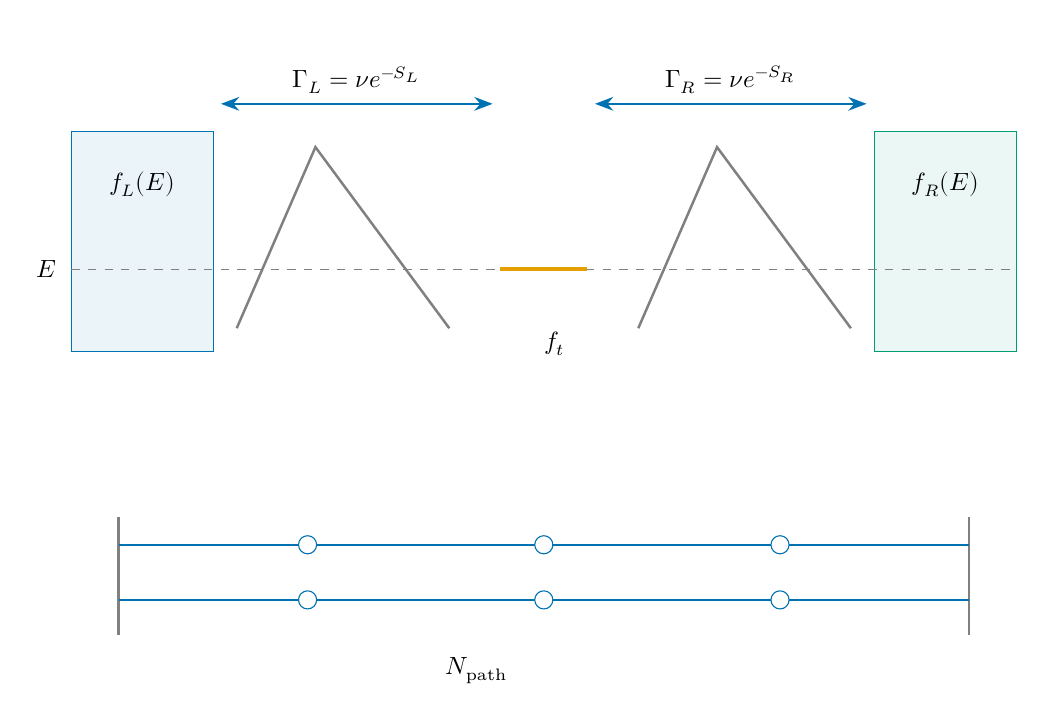
\begin{tikzpicture}[x=1cm,y=1cm,font=\small,
box/.style={draw=tolblue,line width=.75pt,fill=tolblue!3,align=center,inner sep=7pt},
arr/.style={-{Stealth},line width=.85pt,draw=tolblue},
rev/.style={-{Stealth},line width=.75pt,draw=tolorange},
both/.style={<->,>=Stealth,line width=.8pt,draw=tolblue}]

\node[font=\bfseries]at(6,4.0){{\cjkfont 上：固定电子能量下的顺序微结（能量高度任意）}};
\draw[fill=tolblue!8,draw=tolblue](0,0)rectangle(1.8,2.8);
\draw[fill=tolgreen!8,draw=tolgreen](10.2,0)rectangle(12,2.8);
\node[align=center]at(.9,2.2){{\cjkfont 左有效库}\\$f_L(E)$};
\node[align=center]at(11.1,2.2){{\cjkfont 右有效库}\\$f_R(E)$};
\draw[draw=gray,line width=.9pt](2.1,.3)--(3.1,2.6)--(4.8,.3);
\draw[draw=gray,line width=.9pt](7.2,.3)--(8.2,2.6)--(9.9,.3);
\draw[dashed,gray](0,1.05)--(12,1.05);
\node[anchor=east]at(-.08,1.05){$E$};
\draw[tolorange,line width=1.3pt](5.45,1.05)--(6.55,1.05);
\node[align=center]at(6,.1){{\cjkfont 陷阱}\ $f_t$};
\draw[both](1.9,3.15)--node[above]{$\Gamma_L=\nu e^{-S_L}$}(5.35,3.15);
\draw[both](6.65,3.15)--node[above]{$\Gamma_R=\nu e^{-S_R}$}(10.1,3.15);
\node at(6,-.85){{\cjkfont 两库交换同一电子；不是额外的体产对}};
\draw[gray,line width=.85pt](.6,-2.1)--(.6,-3.6);
\draw[gray,line width=.85pt](11.4,-2.1)--(11.4,-3.6);
\foreach \yy in {-2.45,-3.15}{
 \draw[tolblue,line width=.8pt](.6,\yy)--(11.4,\yy);
 \foreach \xx in {3,6,9}{\node[circle,fill=white,draw=tolblue,minimum size=.23cm,inner sep=0pt]at(\xx,\yy){};}
}
\node at(6,-1.70){{\cjkfont 下：完整并联路径的几何计数示意}};
\node at(6,-4.05){{$N_{\rm path}$ {\cjkfont 数贯通通道的面密度，不数每个串联微结}}};
\end{tikzpicture}}
\caption{{\cjkfont 上半图仅说明固定能量}\allowbreak{}E\allowbreak{}{\cjkfont 的电子通过两侧空间势垒，与一个陷阱顺序交换；}\allowbreak{}\ensuremath{\Gamma}\allowbreak{}{\cjkfont 描述隧穿交换强度，实际进出还受储库费米占据与陷阱空满限制。折线势垒是概念草图，不是重新计算或实测势形，也不表示左右事件相干同时发生。下半图的两条线仅作计数例子：每条贯通路径可以含多个串联微结，不能把全部微结都当成独立并联通道。因此体陷阱数乘厚度不自动等于}\allowbreak{}Npath\nobreak{}{\cjkfont 。含多个串联微结的路径还需联合求解占据与交换，不能直接复用上方单微结的净率。}\allowbreak{}}\label{fig:25}
{\footnotesize\color{SourceGray} {\cjkfont 独立}\allowbreak{}tat\_\allowbreak{}model.py\allowbreak{}{\cjkfont 及解析}\allowbreak{}WKB\allowbreak{}{\cjkfont 核验}\allowbreak{} \cite{D0}\nobreak{}{\cjkfont ；声子辅助深中心过程背景}\allowbreak{} \cite{R9a} \cite{R9b}\par}
\end{figure}
\medskip
% ===== FROZEN SECTION 33 =====
\FloatBarrier
\Needspace{110pt}
\section{{\cjkfont 弹性}\allowbreak{}TAT\allowbreak{}{\cjkfont 例子并没有同时解释所有现象}\allowbreak{}}\label{sec:33}
% SOURCE 33-paragraph-0 2bb61f3605de68718eb4ca0abf45a352978fbddfbcc447f28ddc0c3faad775ac
{\cjkfont 原}\allowbreak{}TAT\allowbreak{}{\cjkfont 示例取每段}\allowbreak{}2 nm\nobreak{}{\cjkfont 、有效质量}\allowbreak{}0.2me\nobreak{}{\cjkfont 、势垒}\allowbreak{}0.65 eV\nobreak{}{\cjkfont 、陷阱高斯宽}\allowbreak{}0.08 eV\nobreak{}{\cjkfont 、尝试频率}\allowbreak{}10\textsuperscript{12} s\textsuperscript{−1}\allowbreak{}{\cjkfont 和}\allowbreak{}Npath=\allowbreak{}10\textsuperscript{9} cm\textsuperscript{−2}\nobreak{}{\cjkfont 。所有这些都是探索值，并非从}\allowbreak{}D18:L8-BO\allowbreak{}{\cjkfont 测得。势垒长度与质量共同进入}\allowbreak{}WKB\allowbreak{}{\cjkfont 作用量，单条曲线无法唯一辨认二者。}\allowbreak{}
\par
% SOURCE 33-paragraph-1 491d37607be843a0395a57cc1ccfd0afba44c51caf8f15de1c2fd2733cf9c6ec
{\cjkfont 在}\allowbreak{}100 nm\nobreak{}{\cjkfont 、}\allowbreak{}300 K\allowbreak{}{\cjkfont 的}\allowbreak{}FF78\allowbreak{}{\cjkfont 参照上并入此支路，}\allowbreak{}FF\allowbreak{}{\cjkfont 降为}\allowbreak{}53.69\%\nobreak{}{\cjkfont ，}\allowbreak{}V50\allowbreak{}{\cjkfont 约}\allowbreak{}−3.088 V\nobreak{}{\cjkfont ，三厚度}\allowbreak{}K50\allowbreak{}{\cjkfont 约}\allowbreak{}0.03056 V/nm\nobreak{}{\cjkfont 。高场曲线还出现回落，}\allowbreak{}V75\allowbreak{}{\cjkfont 未达到。这说明一个可以产生反向大电流的通道，也可能过早破坏正向工作区，不能只看反向上翘就称解释成功。}\allowbreak{}
\par
% SOURCE 33-paragraph-2 5d6b631e613d74e2deae80f8dc2a3f05c3f09db327802daf0f6861ed2fd5a813
{\cjkfont 本次温度审计又重新调用该弹性支路：}\allowbreak{}0.1 MV/cm\allowbreak{}{\cjkfont 的}\allowbreak{}80/300 K\allowbreak{}{\cjkfont 电流约}\allowbreak{}9.698/8.765 mA/cm\textsuperscript{2}\nobreak{}{\cjkfont ；}\allowbreak{}1 MV/cm\allowbreak{}{\cjkfont 约}\allowbreak{}47.719/46.671 mA/cm\textsuperscript{2}\nobreak{}{\cjkfont 。}\allowbreak{}\ensuremath{\Gamma}\allowbreak{}{\cjkfont 即使没有显式温度项，费米占据窗口仍会带来温度变化，所以“隧穿温度无关”不是完整器件电流的普遍结论。}\allowbreak{}
\par
% SOURCE 33-paragraph-3 2e3b5e81dccee8adf27371dc28d75218cc097037e43077156279deda19be97ea
{\cjkfont 下一步若保留这个候选，应显式加入可用带边、归一}\allowbreak{}DOS\nobreak{}{\cjkfont 、声子过程和真实空间供给，随后再与}\allowbreak{}DD\allowbreak{}{\cjkfont 电荷及电势联立。不能添加任意}\allowbreak{}Arrhenius\allowbreak{}{\cjkfont 倍率，只为把温度趋势改成预期方向。}\allowbreak{}
\par
\begin{figure}[!htbp]
\centering
\includegraphics[width=.90\linewidth,height=.38\textheight,keepaspectratio]{figures/tat.pdf}
\caption{{\cjkfont 存档顺序}\allowbreak{}WKB\allowbreak{}{\cjkfont 缩约通道：默认参数均未标定，新增电流与}\allowbreak{}FF78\allowbreak{}{\cjkfont 局域}\allowbreak{}DD\allowbreak{}{\cjkfont 支路相加。图中回落和未跨阈值同样保留。}\allowbreak{}}\label{fig:26}
{\footnotesize\color{SourceGray} TAT\_\allowbreak{}MODEL\_\allowbreak{}REPORT\allowbreak{}{\cjkfont 与}\allowbreak{}tat\_\allowbreak{}results \cite{D0}\nobreak{}{\cjkfont ；独立低温占据诊断}\allowbreak{} \cite{D3}\par}
\end{figure}
\medskip
% ===== FROZEN SECTION 34 =====
\FloatBarrier
\Needspace{110pt}
\section{{\cjkfont 接触注入能画上翘但还未闭合空间电荷}\allowbreak{}}\label{sec:34}
% SOURCE 34-paragraph-0 501461c8ea79272b3ac5341f5079ebb62c4509c4b5361c823eb57219fbb6cb6c
{\cjkfont 原接触候选采用对称有效}\allowbreak{}Schottky\allowbreak{}{\cjkfont 并联支路：势垒受外加名义场降低，热发射尺度乘以一个}\allowbreak{}tanh\allowbreak{}{\cjkfont 净流因子，使零偏电流为零、正反偏具有对称响应。默认势垒}\allowbreak{}0.60 eV\nobreak{}{\cjkfont 、前因子}\allowbreak{}10\textsuperscript{4} A/cm\textsuperscript{2}\nobreak{}{\cjkfont ，均是探索参数，不是测得的有机}\allowbreak{}Richardson\allowbreak{}{\cjkfont 常数。}\allowbreak{}
\par
% SOURCE 34-paragraph-1 e1e977a231c916d7baca0b97c903ad1bfc110179c65644b3bf4ddae276ad69b6
{\cjkfont 该示例给}\allowbreak{}FF\allowbreak{}{\cjkfont 约}\allowbreak{}77.97\%\nobreak{}{\cjkfont 、}\allowbreak{}V50\ensuremath{\approx}\allowbreak{}−17.288 V\nobreak{}{\cjkfont 、}\allowbreak{}K50\ensuremath{\approx}\allowbreak{}0.1727 V/nm\nobreak{}{\cjkfont 。改变注入势垒可以明显移动反向阈值，但对正向}\allowbreak{}FF\allowbreak{}{\cjkfont 影响很小。这种差异本身有信息量：若实验}\allowbreak{}FF\allowbreak{}{\cjkfont 跨度很大，还需界面复合或提取变化，不能只靠当前并联支路解释所有关联。}\allowbreak{}
\par
% SOURCE 34-paragraph-2 37ce550770cd3e9f90de725147690b30c81f0a00110d82ebeb49ac43c00599f3
{\cjkfont 数学上，支路电流由外部储库供给，并满足被设定的端口对称性；器件物理上，它没有把注入电荷重新送入}\allowbreak{}Poisson\allowbreak{}{\cjkfont 和连续性求解，没有解析势垒的空间形状、局部带尾或接触附近复合。因此不能把该图当成完整注入机制已经被验证。}\allowbreak{}
\par
% SOURCE 34-paragraph-3 77e6d2fce23f7583202873f4a9b10ab0ade7df673afa6558578d3c5bd524b05c
{\cjkfont 已核的}\allowbreak{}PDINN\allowbreak{}{\cjkfont 原始研究表明，界面层可以显著改变}\allowbreak{}Ag\allowbreak{}{\cjkfont 功函数。它支持接触值得研究，却不意味着用户器件的}\allowbreak{}0.60 eV\allowbreak{}{\cjkfont 有效势垒已经被测量。未来真正的接触比较应在相同材料能级、局部谱和边界电化学势下进行。}\allowbreak{}
\par
\begin{equation}
J_{\mathrm{inj}}=J_{00}\left(\frac{T}{300}\right)^2 e^{-\max(\Phi-\Delta_S,0)/(k_BT)}\tanh\!\left(\frac{V}{2nk_BT}\right)
\label{eq:38}\end{equation}
\begin{center}\begin{minipage}{\linewidth}\small
\setlength{\TableWidth}{\dimexpr\linewidth-2\tabcolsep\relax}
\begin{tabular}{@{}>{\raggedright\arraybackslash}p{0.360\TableWidth}>{\raggedright\arraybackslash}p{0.640\TableWidth}@{}}
\toprule
\bfseries {\cjkfont 当前支路已包含}\allowbreak{} & \bfseries {\cjkfont 尚未包含}\allowbreak{}\\\midrule
{\cjkfont 外加名义场与有效降垒}\allowbreak{} & {\cjkfont 自洽注入空间电荷}\allowbreak{}\\[3pt]
{\cjkfont 有限势垒和温度因子}\allowbreak{} & {\cjkfont 真实有机界面}\allowbreak{}DOS\\[3pt]
{\cjkfont 零偏净流为零}\allowbreak{} & {\cjkfont 逐空间位置的产生复合}\allowbreak{}\\[3pt]
{\cjkfont 与基准端口电流相加}\allowbreak{} & {\cjkfont 新边界与}\allowbreak{}DD\allowbreak{}{\cjkfont 联合求解}\allowbreak{}\\[3pt]
\bottomrule\end{tabular}
\par\vspace{6pt}{\footnotesize\color{SourceGray} reduced\_\allowbreak{}models.py\allowbreak{}{\cjkfont 及存档比较}\allowbreak{} \cite{D0}\nobreak{}{\cjkfont ；}\allowbreak{}PDINN\allowbreak{}{\cjkfont 界面原始证据}\allowbreak{} \cite{R13}\par}
\end{minipage}\end{center}
\medskip
% ===== FROZEN SECTION 35 =====
\FloatBarrier
\Needspace{110pt}
\section{{\cjkfont 电热反馈有自己的动力学与稳定性}\allowbreak{}}\label{sec:35}
% SOURCE 35-paragraph-0 ae5eb52c8c33a2486dfcdc45d3a6a0f1601495d0c026d3fade7ee66d2347b9a1
{\cjkfont 热模型把吸收光功率与端口电功率加入温度方程，再用热阻将能量散向环境。反偏时}\allowbreak{}V\allowbreak{}{\cjkfont 和}\allowbreak{}J\allowbreak{}{\cjkfont 同号，}\allowbreak{}VJ\allowbreak{}{\cjkfont 为正；发电区}\allowbreak{}VJ\allowbreak{}{\cjkfont 为负，代表电能输出。漏电导随温度增加，温升又增加漏电，于是可能形成正反馈。这个机制不需要把每次载流子加速都叫作雪崩。}\allowbreak{}
\par
% SOURCE 35-paragraph-1 990dc285f7e0fc84cdc4f9b110b2683a8e673d5f91bad0f193d4cdd98f672544
{\cjkfont 原示例采用}\allowbreak{}Rth=\allowbreak{}100 K·cm\textsuperscript{2}/W\nobreak{}{\cjkfont 、面积热容}\allowbreak{}0.02 J/(cm\textsuperscript{2}·K)\nobreak{}{\cjkfont 、吸收}\allowbreak{}0.08 W/cm\textsuperscript{2}\allowbreak{}{\cjkfont 和漏电激活能}\allowbreak{}0.55 eV\nobreak{}{\cjkfont 。零偏光照初温约}\allowbreak{}308 K\nobreak{}{\cjkfont ，默认}\allowbreak{}2 V/s\allowbreak{}{\cjkfont 反扫给}\allowbreak{}V50\ensuremath{\approx}\allowbreak{}−11.742 V\nobreak{}{\cjkfont 。}\allowbreak{}430 K\allowbreak{}{\cjkfont 仅是模型有效温区的计算停止点，没有损伤变量，不能称为烧毁温度。}\allowbreak{}
\par
% SOURCE 35-paragraph-2 a89ed8f094976fbb22aaf2a946c8422a61790f026056ab858972bb26aa615ed7
{\cjkfont 稳态热平衡是功率净流为零；局部稳定还要求升温时净输入下降。瞬态扫描可能滞后于稳态分支，所以脉冲长度、扫描速度和初始温度会影响曲线。相反，}\allowbreak{}Newton\allowbreak{}{\cjkfont 在某电压不收敛并不等于这条热稳定条件被违反。}\allowbreak{}
\par
% SOURCE 35-paragraph-3 36570a6200715ec50f2b2b1c384b80b91d7a22efc57ff3d1f605e0528db3f0dd
{\cjkfont 当前模型是集总温度，不解析局部热点或热界面；}\allowbreak{}K50\allowbreak{}{\cjkfont 接近零也与}\allowbreak{}Rth\allowbreak{}{\cjkfont 及漏电支路不随厚度变化有关。它不排除别的热边界下存在厚度比例关系，更不能因液氮浴稳定就排除薄膜局部自热。}\allowbreak{}
\par
\begin{equation}
C_A\dot T=P_{\mathrm{abs}}+VJ(V,T)-\frac{T-T_b}{R_A}
\label{eq:39}\end{equation}
\begin{equation}
\mathrm{steady}:\ H(T)=0,\qquad\mathrm{stable}:\ \partial_T H<0
\label{eq:40}\end{equation}
\begin{figure}[!htbp]
\centering
\includegraphics[width=.90\linewidth,height=.38\textheight,keepaspectratio]{figures/thermal.pdf}
\caption{{\cjkfont 存档集总电热扫描。不同扫描速率是物理时间协议；达到}\allowbreak{}430 K\allowbreak{}{\cjkfont 按有效域停止，图中停止不等于不可逆损伤。}\allowbreak{}}\label{fig:27}
{\footnotesize\color{SourceGray} {\cjkfont 热方程、初态及停止条件}\allowbreak{} \cite{D0}\par}
\end{figure}
\medskip
% ===== FROZEN SECTION 36 =====
\FloatBarrier
\Needspace{110pt}
\section{{\cjkfont 弱区与经验支路分别能说明多少}\allowbreak{}}\label{sec:36}
% SOURCE 36-paragraph-0 815c854fe07a93c7f316ced259271f963048c27f5549fdcd32481736727c7519
{\cjkfont 弱区模型把器件看成良好区域与少量差区域的并联。差区域有自己的较薄}\allowbreak{}DD\allowbreak{}{\cjkfont 列、更高陷阱及附加注入、欧姆泄漏；每个局部电流先按局部面积定义，再乘面积比例。这能说明少量薄区或缺陷如何拉低}\allowbreak{}FF\allowbreak{}{\cjkfont 并提前反向增长。}\allowbreak{}
\par
% SOURCE 36-paragraph-1 625eb43622e7117b0a09052ac4a001511668d22d52c2b7c7c5e324c1fe079421
{\cjkfont 原默认弱区比例}\allowbreak{}1\%\nobreak{}{\cjkfont 、厚度为良区一半，给}\allowbreak{}FF\allowbreak{}{\cjkfont 约}\allowbreak{}76.52\%\nobreak{}{\cjkfont 、}\allowbreak{}V50\ensuremath{\approx}\allowbreak{}−17.090 V\nobreak{}{\cjkfont 、}\allowbreak{}K50\ensuremath{\approx}\allowbreak{}0.1594 V/nm\nobreak{}{\cjkfont 。它没有横向电场集中、热点迁移、随机缺陷分布或导电丝生长，因此只能作面积加权的存在性例子，不能称为微观击穿通道重建。}\allowbreak{}
\par
% SOURCE 36-paragraph-2 f211d7a4d441a1d8b96bc743d5036420eaa156e154aef3645ddff74271d546ac
{\cjkfont 经验支路}\allowbreak{}J=\allowbreak{}GVexp(−V0/\ensuremath{\vert}V\ensuremath{\vert})\allowbreak{}{\cjkfont 则更直接：它可以描述随电压急剧增大的被动漏电，并与基准光伏电流相加。默认例子几乎保持}\allowbreak{}78\%FF\nobreak{}{\cjkfont ，}\allowbreak{}V50\allowbreak{}{\cjkfont 约}\allowbreak{}−17.036 V\nobreak{}{\cjkfont ，但}\allowbreak{}K50\allowbreak{}{\cjkfont 近零，因为该函数的关键尺度是电压而非场。}\allowbreak{}
\par
% SOURCE 36-paragraph-3 4cfe77ba766993eae160e006127ef80df37f8005ea9525e934c419c2b066143c
{\cjkfont 经验拟合不是没有用。它能压缩曲线、比较阈值和提供插值；错误在于把一个拟合电压尺度}\allowbreak{}V0\allowbreak{}{\cjkfont 自动解释成陷阱深度或隧穿长度。本项目的科学目标要求“曲线描述有效”与“微观解释成立”分开记分。}\allowbreak{}
\par
\begin{equation}
J_{\mathrm{area}}=(1-f_A)J_{\mathrm{good}}+f_AJ_{\mathrm{bad}}
\label{eq:41}\end{equation}
\begin{equation}
J_{\mathrm{emp}}=GV\exp[-V_0/|V|]
\label{eq:42}\end{equation}
\begin{figure}[!htbp]
\centering
\resizebox{.90\linewidth}{!}{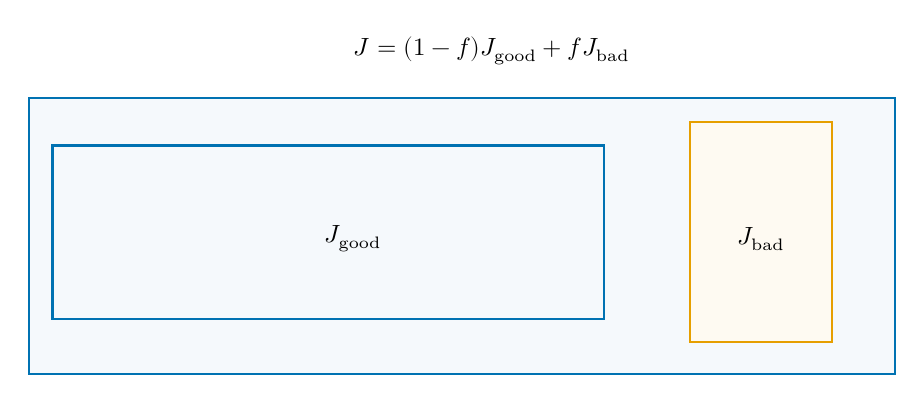
\begin{tikzpicture}[x=1cm,y=1cm,box/.style={draw=tolblue,fill=tolblue!4,line width=.8pt,align=center,inner sep=8pt,font=\small},bi/.style={<->,>=Stealth,line width=.85pt,draw=tolblue}]

\draw[draw=tolblue,fill=tolblue!4,line width=.9pt] (0,0) rectangle(11,3.5);
\node[box,minimum width=7cm,minimum height=2.2cm] at(3.8,1.8) {{\cjkfont 良好区域}\\{\cjkfont 局部面积电流} $J_{\rm good}$};
\node[box,draw=tolorange,fill=tolorange!5,minimum width=1.8cm,minimum height=2.8cm] at(9.3,1.8) {{\cjkfont 弱区}\\$J_{\rm bad}$};
\node[font=\small] at(5.5,4.1) {{\cjkfont 总面积归一}\quad $J=(1-f)J_{\rm good}+fJ_{\rm bad}$};
\end{tikzpicture}}
\caption{{\cjkfont 原创弱区示意：局部电流必须先按各自面积归一；简单并联不包含横向电势与空间热点。}\allowbreak{}}\label{fig:28}
{\footnotesize\color{SourceGray} {\cjkfont 缩约弱区、经验支路源码与存档结果}\allowbreak{} \cite{D0}\par}
\end{figure}
\medskip
% ===== FROZEN SECTION 37 =====
\clearpage
\part*{{\cjkfont 第四部分}\allowbreak{} \allowbreak{}{\cjkfont 材料约束与低温理论}\allowbreak{}}
\FloatBarrier
\Needspace{110pt}
\section{{\cjkfont 材料能级存在多种测量口径}\allowbreak{}}\label{sec:37}
% SOURCE 37-paragraph-0 b9d7c9a90e57cbeeb0f705f739ee20d7b4799cb57e5e802b2560a308fb317c6e
D18:L8-BO\allowbreak{}{\cjkfont 不是一个唯一能级数字。最常见的误用是从不同论文各取一个}\allowbreak{}HOMO\allowbreak{}{\cjkfont 或}\allowbreak{}LUMO\nobreak{}{\cjkfont ，再相减称为测得的输运隙，随后同时控制}\allowbreak{}ni\nobreak{}{\cjkfont 、接触与陷阱深度。}\allowbreak{}CV\nobreak{}{\cjkfont 、}\allowbreak{}UPS\nobreak{}{\cjkfont 、}\allowbreak{}PESA\allowbreak{}{\cjkfont 和}\allowbreak{}IPES\allowbreak{}{\cjkfont 的对象、环境与推算步骤并不完全相同；纯膜前沿差也不等于共混界面的}\allowbreak{}CT\allowbreak{}{\cjkfont 自由能。}\allowbreak{}
\par
% SOURCE 37-paragraph-1 2d2fd0ace042da1cfb867221e15966133baa3ab9d1608099b139884cbf950ad6
{\cjkfont 原}\allowbreak{}D18\allowbreak{}{\cjkfont 论文}\allowbreak{}CV\allowbreak{}{\cjkfont 给}\allowbreak{}HOMO−5.51 eV\nobreak{}{\cjkfont ；}\allowbreak{}L8-BO\allowbreak{}{\cjkfont 原始论文}\allowbreak{}CV\allowbreak{}{\cjkfont 给}\allowbreak{}LUMO−3.90 eV\nobreak{}{\cjkfont ，两者相减为}\allowbreak{}1.61 eV\nobreak{}{\cjkfont 。另一篇同文}\allowbreak{}PESA/IPES\allowbreak{}{\cjkfont 表列}\allowbreak{}D18−5.39\nobreak{}{\cjkfont 、}\allowbreak{}L8-BO−3.98 eV\nobreak{}{\cjkfont ，差}\allowbreak{}1.41 eV\nobreak{}{\cjkfont 。}\allowbreak{}2026\allowbreak{}{\cjkfont 年}\allowbreak{}UPS\allowbreak{}{\cjkfont 结合}\allowbreak{}CV\allowbreak{}{\cjkfont 隙推算的一组值则给差}\allowbreak{}1.64 eV\nobreak{}{\cjkfont ；其中}\allowbreak{}L8-BO\allowbreak{}{\cjkfont 的}\allowbreak{}−3.45 eV\allowbreak{}{\cjkfont 并非}\allowbreak{}IPES\allowbreak{}{\cjkfont 直接测得。}\allowbreak{}
\par
% SOURCE 37-paragraph-2 51467ecff22a83159603457c06b271eb8830825d7e4f0cbcb66e2f347449d6f3
{\cjkfont 这三个数是方法分支，不是可以平均的误差条。若进入}\allowbreak{}ni\allowbreak{}{\cjkfont 的自由电荷差从}\allowbreak{}1.30\allowbreak{}{\cjkfont 改成}\allowbreak{}1.61 eV\nobreak{}{\cjkfont ，在其它量固定时}\allowbreak{}300 K\allowbreak{}{\cjkfont 的}\allowbreak{}ni\allowbreak{}{\cjkfont 就缩为约}\allowbreak{}0.00249\allowbreak{}{\cjkfont 倍，}\allowbreak{}ni\textsuperscript{2}\allowbreak{}{\cjkfont 为}\allowbreak{}6.20\ensuremath{\times}10\textsuperscript{−6}\allowbreak{}{\cjkfont 倍。用}\allowbreak{}Nt\allowbreak{}{\cjkfont 或}\allowbreak{}c\allowbreak{}{\cjkfont 重新拟合可以掩盖口径错误，因此能量定义必须先于曲线调参。}\allowbreak{}
\par
% SOURCE 37-paragraph-3 5cb4270a724a94fcb632368a85a8db028a9238448311b6c1616a51894f57fbe3
{\cjkfont 本书不选择一个“正确新}\allowbreak{}Eg\nobreak{}{\cjkfont ”替代原值。目标}\allowbreak{}Efree\nobreak{}{\cjkfont 、}\allowbreak{}ECT\nobreak{}{\cjkfont 、缺陷电荷转换能仍分开留空；旧}\allowbreak{}1.3 eV\allowbreak{}{\cjkfont 只保留为构造基准。}\allowbreak{}
\par
\begin{equation}
\frac{n_i(E_2)}{n_i(E_1)}=e^{-(E_2-E_1)/(2k_BT)}
\label{eq:43}\end{equation}
\begin{center}\begin{minipage}{\linewidth}\small
\setlength{\TableWidth}{\dimexpr\linewidth-6\tabcolsep\relax}
\begin{tabular}{@{}>{\raggedright\arraybackslash}p{0.290\TableWidth}>{\raggedright\arraybackslash}p{0.240\TableWidth}>{\raggedright\arraybackslash}p{0.250\TableWidth}>{\raggedright\arraybackslash}p{0.220\TableWidth}@{}}
\toprule
\bfseries {\cjkfont 能级来源}\allowbreak{} & \bfseries D18 HOMO & \bfseries L8-BO LUMO & \bfseries {\cjkfont 差值}\allowbreak{}\\\midrule
{\cjkfont 跨文献}\allowbreak{}CV & −5.51 & −3.90 & 1.61 eV\\[3pt]
{\cjkfont 同文}\allowbreak{}PESA/IPES & −5.39 & −3.98 & 1.41 eV\\[3pt]
UPS\allowbreak{}{\cjkfont 加}\allowbreak{}CV\allowbreak{}{\cjkfont 隙推算}\allowbreak{} & −5.09 & −3.45 \allowbreak{}{\cjkfont 推算}\allowbreak{} & 1.64 eV\\[3pt]
\bottomrule\end{tabular}
\par\vspace{6pt}{\footnotesize\color{SourceGray} {\cjkfont 原始能级和处理口径}\allowbreak{} \cite{R11} \cite{R12} \cite{R15} \cite{R16}\nobreak{}{\cjkfont ；材料审计}\allowbreak{} \cite{D5}\par}
\end{minipage}\end{center}
\medskip
% ===== FROZEN SECTION 38 =====
\FloatBarrier
\Needspace{110pt}
\section{{\cjkfont 迁移率必须作为成套文献场景使用}\allowbreak{}}\label{sec:38}
% SOURCE 38-paragraph-0 cdea191d833ec927a2858e752933226e10a8a38dfd8155e1ffdbf5db1c4cdd5d
{\cjkfont 最接近当前质量比的原始来源为}\allowbreak{}Zhu\allowbreak{}{\cjkfont 等}\allowbreak{}2022\allowbreak{}{\cjkfont 年正式}\allowbreak{}SI\nobreak{}{\cjkfont ：}\allowbreak{}D18:L8-BO=\allowbreak{}1:1.2\nobreak{}{\cjkfont 、单载流子膜约}\allowbreak{}120 nm\nobreak{}{\cjkfont ，含陷阱}\allowbreak{}DD\allowbreak{}{\cjkfont 反演得到}\allowbreak{}trap-free \ensuremath{\mu}e=\allowbreak{}1.40\ensuremath{\times}10\textsuperscript{−3}\nobreak{}{\cjkfont 、}\allowbreak{}\ensuremath{\mu}h=\allowbreak{}1.80\ensuremath{\times}10\textsuperscript{−3} cm\textsuperscript{2}/Vs\nobreak{}{\cjkfont 。它与直接}\allowbreak{}Mott–Gurney\allowbreak{}{\cjkfont 斜率的“有效迁移率”不是同一个观测量。}\allowbreak{}
\par
% SOURCE 38-paragraph-1 e7451e5a1a072616989360759a17edb3eb3b0a39c08e5aaee4829ffd84bbf1cb
{\cjkfont 另一项}\allowbreak{}1:1.5\nobreak{}{\cjkfont 、}\allowbreak{}88 nm\allowbreak{}{\cjkfont 研究给}\allowbreak{}\ensuremath{\mu}e\allowbreak{}{\cjkfont 约}\allowbreak{}9.63\ensuremath{\times}10\textsuperscript{−4}\nobreak{}{\cjkfont 、}\allowbreak{}\ensuremath{\mu}h\allowbreak{}{\cjkfont 约}\allowbreak{}4.98\ensuremath{\times}10\textsuperscript{−5}\nobreak{}{\cjkfont ，电子空穴比约}\allowbreak{}19\nobreak{}{\cjkfont ；}\allowbreak{}1:1.4\allowbreak{}{\cjkfont 研究给}\allowbreak{}4.39\ensuremath{\times}10\textsuperscript{−4}\allowbreak{}{\cjkfont 和}\allowbreak{}2.71\ensuremath{\times}10\textsuperscript{−4}\nobreak{}{\cjkfont ，比约}\allowbreak{}1.62\nobreak{}{\cjkfont 。同一材料名下出现不同失衡程度并不奇怪，因为制程、接触、膜厚及反演假设都参与决定。}\allowbreak{}
\par
% SOURCE 38-paragraph-2 93d759aa43d4a7349fa48156117329b39221f5e7975a5c8d9c1b73f2781e05f9
SCLC\allowbreak{}{\cjkfont 关系中}\allowbreak{}\ensuremath{\mu}\allowbreak{}{\cjkfont 与所取介电常数、}\allowbreak{}d\textsuperscript{3}\allowbreak{}{\cjkfont 和有效电压相关。把一篇的}\allowbreak{}\ensuremath{\mu}e\nobreak{}{\cjkfont 、另一篇的}\allowbreak{}\ensuremath{\mu}h\nobreak{}{\cjkfont 、第三篇的}\allowbreak{}\ensuremath{\varepsilon}\allowbreak{}{\cjkfont 拼成“最佳参数组”，会丢掉这些条件关联。更合理的是保留成对场景，并明确它们不是当前器件标定。}\allowbreak{}
\par
% SOURCE 38-paragraph-3 388a2c97099cd467e725f10990ce3327bf58661cee329966e3db1fe091dceac9
{\cjkfont 文献}\allowbreak{}\ensuremath{\varepsilon}r=\allowbreak{}4.36\allowbreak{}{\cjkfont 来自一种不同接触工艺的频率依赖电容；}\allowbreak{}2022\allowbreak{}{\cjkfont 年}\allowbreak{}DD\allowbreak{}{\cjkfont 中的}\allowbreak{}\ensuremath{\varepsilon}r=\allowbreak{}3\allowbreak{}{\cjkfont 却是固定输入。低频器件介电响应也不能自动当作亚纳米缺陷快速转移的局部屏蔽。当前}\allowbreak{}FF78 \ensuremath{\mu}\ensuremath{\approx}\allowbreak{}0.00452\allowbreak{}{\cjkfont 较上述同质量比文献值高约}\allowbreak{}2.5–3.2\allowbreak{}{\cjkfont 倍，但本来就是}\allowbreak{}FF\allowbreak{}{\cjkfont 构造值，不能误指其曾宣称实测。}\allowbreak{}
\par
\begin{center}\begin{minipage}{\linewidth}\small
\setlength{\TableWidth}{\dimexpr\linewidth-6\tabcolsep\relax}
\begin{tabular}{@{}>{\raggedright\arraybackslash}p{0.340\TableWidth}>{\raggedright\arraybackslash}p{0.200\TableWidth}>{\raggedright\arraybackslash}p{0.230\TableWidth}>{\raggedright\arraybackslash}p{0.230\TableWidth}@{}}
\toprule
\bfseries {\cjkfont 分支}\allowbreak{} & \bfseries \ensuremath{\mu}e & \bfseries \ensuremath{\mu}h & \bfseries {\cjkfont 性质}\allowbreak{}\\\midrule
1:1.2 120 nm & 1.40\ensuremath{\times}10\textsuperscript{−3} & 1.80\ensuremath{\times}10\textsuperscript{−3} & {\cjkfont 含陷阱}\allowbreak{}DD\allowbreak{}{\cjkfont 反演}\allowbreak{}\\[3pt]
1:1.5 88 nm & 9.63\ensuremath{\times}10\textsuperscript{−4} & 4.98\ensuremath{\times}10\textsuperscript{−5} & {\cjkfont 有效}\allowbreak{}SCLC\\[3pt]
1:1.4 & 4.39\ensuremath{\times}10\textsuperscript{−4} & 2.71\ensuremath{\times}10\textsuperscript{−4} & {\cjkfont 有效}\allowbreak{}SCLC\\[3pt]
FF78\allowbreak{}{\cjkfont 构造}\allowbreak{} & 4.525\ensuremath{\times}10\textsuperscript{−3} & 4.525\ensuremath{\times}10\textsuperscript{−3} & {\cjkfont 非材料标定}\allowbreak{}\\[3pt]
\bottomrule\end{tabular}
\par\vspace{6pt}{\footnotesize\color{SourceGray} \ensuremath{\mu}\allowbreak{}{\cjkfont 单位均为}\allowbreak{}cm\textsuperscript{2}/Vs\nobreak{}{\cjkfont ；原始来源}\allowbreak{} \cite{R17} \cite{R18} \cite{R19} \cite{R20}\nobreak{}{\cjkfont ；}\allowbreak{}23\allowbreak{}{\cjkfont 行证据}\allowbreak{} \cite{D5}\par}
\end{minipage}\end{center}
\medskip
% ===== FROZEN SECTION 39 =====
\FloatBarrier
\Needspace{110pt}
\section{{\cjkfont 浅陷阱}\allowbreak{} \allowbreak{}{\cjkfont 光学尾与深中心不是同一参数}\allowbreak{}}\label{sec:39}
% SOURCE 39-paragraph-0 9e060ee6cbaf6e697cbd9dfc60672f48a9295ffdd7d55f47dfe9dd207881a144
2022\allowbreak{}{\cjkfont 年同质量比研究用}\allowbreak{}C–f\allowbreak{}{\cjkfont 估计局域高斯陷阱总密度约}\allowbreak{}3.76\ensuremath{\times}10\textsuperscript{15} cm\textsuperscript{−3}\nobreak{}{\cjkfont 、带边深度}\allowbreak{}0.164 eV\nobreak{}{\cjkfont 、宽度}\allowbreak{}18 meV\nobreak{}{\cjkfont ，再作为}\allowbreak{}DD\allowbreak{}{\cjkfont 输入反演}\allowbreak{}SCLC\nobreak{}{\cjkfont 。这些是}\allowbreak{}electron\allowbreak{}{\cjkfont 或}\allowbreak{}hole\allowbreak{}{\cjkfont 各自的}\allowbreak{}Gaussian\allowbreak{}{\cjkfont 输入，并非已证明一个中心负责两支跨隙产生。整套反演还固定}\allowbreak{}Eg=\allowbreak{}1.32 eV\nobreak{}{\cjkfont 、}\allowbreak{}\ensuremath{\varepsilon}r=\allowbreak{}3\nobreak{}{\cjkfont 、}\allowbreak{}Nc/Nv=\allowbreak{}10\textsuperscript{20} cm\textsuperscript{−3}\allowbreak{}{\cjkfont 及捕获截面。同篇另有阻抗输运}\allowbreak{}DOS\allowbreak{}{\cjkfont 无序度}\allowbreak{}66.8 meV\nobreak{}{\cjkfont ；另一篇}\allowbreak{}s-EQE\allowbreak{}{\cjkfont 光学尾给}\allowbreak{}Urbach\allowbreak{}{\cjkfont 能}\allowbreak{}26.71 meV\nobreak{}{\cjkfont 。这些值并存，已经说明“宽度}\allowbreak{}\ensuremath{\sigma}\nobreak{}{\cjkfont ”不是一个跨方法通用的数字。}\allowbreak{}
\par
% SOURCE 39-paragraph-1 b252759c08b3a0299d3d257b5e644535483180fd929c7687520ba479732709ff
{\cjkfont 原模型对称中带隙为}\allowbreak{}0.65/0.65 eV\nobreak{}{\cjkfont 。若保持}\allowbreak{}Eg=\allowbreak{}1.3 eV\nobreak{}{\cjkfont ，把电子深度改为}\allowbreak{}0.164 eV\nobreak{}{\cjkfont ，则完整跨隙另一支必须为}\allowbreak{}1.136 eV\nobreak{}{\cjkfont ，不能把两支都变成}\allowbreak{}0.164 eV\nobreak{}{\cjkfont 。如此不对称的诊断电流远小于原模型；这仍不是把浅陷阱身份认定为真正产生中心，而是说明定义不应混用。}\allowbreak{}
\par
% SOURCE 39-paragraph-2 7da946bc7940b61838fa37a71d6ecfed7c115bf1582377d6d4dde1f7dbfff2d1
{\cjkfont 另一个}\allowbreak{}2026\allowbreak{}{\cjkfont 电容}\allowbreak{}DOS\allowbreak{}{\cjkfont 表列}\allowbreak{}5.52\ensuremath{\times}10\textsuperscript{16} cm\textsuperscript{−3} eV\textsuperscript{−1}\nobreak{}{\cjkfont ，正文归一公式却将}\allowbreak{}Nt\allowbreak{}{\cjkfont 称作总密度。单位与归一化存在歧义，不能直接填入积分}\allowbreak{}Nt\nobreak{}{\cjkfont 。该}\allowbreak{}SI\allowbreak{}{\cjkfont 中还出现迁移率比值与两列算术不符，本书保留警告，没有悄悄改原数据。}\allowbreak{}
\par
% SOURCE 39-paragraph-3 2a74df2dc301882b7dbbdd537df2869b84dfeb1720ea80b144dc2dcf21a51051
L8-BO\allowbreak{}{\cjkfont 单晶}\allowbreak{}ZINDO\allowbreak{}{\cjkfont 耦合}\allowbreak{}14.8–19.0 meV\allowbreak{}{\cjkfont 也只属于}\allowbreak{}host–host\allowbreak{}{\cjkfont 堆积。目标缺陷的}\allowbreak{}\ensuremath{\lambda}\nobreak{}{\cjkfont 、}\allowbreak{}H\nobreak{}{\cjkfont 、局域长度、俘获系数、振动谱和图密度仍未测得。保留空值是防止假精确，不是停止理论研究。}\allowbreak{}
\par
\begin{equation}
D_n+D_p=E_g,\qquad 0.164+1.136=1.300\ \mathrm{eV}
\label{eq:44}\end{equation}
\begin{center}\begin{minipage}{\linewidth}\small
\setlength{\TableWidth}{\dimexpr\linewidth-2\tabcolsep\relax}
\begin{tabular}{@{}>{\raggedright\arraybackslash}p{0.360\TableWidth}>{\raggedright\arraybackslash}p{0.640\TableWidth}@{}}
\toprule
\bfseries {\cjkfont 可查到的量}\allowbreak{} & \bfseries {\cjkfont 不能直接替代}\allowbreak{}\\\midrule
{\cjkfont 光学}\allowbreak{}Urbach\allowbreak{}{\cjkfont 能}\allowbreak{}26.71 meV & {\cjkfont 输运}\allowbreak{}Gaussian \ensuremath{\sigma}\\[3pt]
{\cjkfont 局域陷阱宽}\allowbreak{}18 meV & {\cjkfont 重组能}\allowbreak{}\ensuremath{\lambda}\\[3pt]
IS\allowbreak{}{\cjkfont 无序度}\allowbreak{}66.8 meV & {\cjkfont 唯一化学缺陷深度}\allowbreak{}\\[3pt]
{\cjkfont 每}\allowbreak{}eV\allowbreak{}{\cjkfont 的}\allowbreak{}DOS\allowbreak{}{\cjkfont 幅度}\allowbreak{} & {\cjkfont 积分总}\allowbreak{}Nt\\[3pt]
host\allowbreak{}{\cjkfont 单晶耦合}\allowbreak{} & {\cjkfont 缺陷跨隙}\allowbreak{}H\\[3pt]
\bottomrule\end{tabular}
\par\vspace{6pt}{\footnotesize\color{SourceGray} {\cjkfont 材料原文与}\allowbreak{}SI\allowbreak{}{\cjkfont 核对}\allowbreak{} \cite{R12} \cite{R17} \cite{R19} \cite{R20}\nobreak{}{\cjkfont ；缺失项清单}\allowbreak{} \cite{D5}\par}
\end{minipage}\end{center}
\medskip
% ===== FROZEN SECTION 40 =====
\FloatBarrier
\Needspace{110pt}
\section{{\cjkfont 液氮温区首先改变哪些近似}\allowbreak{}}\label{sec:40}
% SOURCE 40-paragraph-0 cf4ae82710de2372fe25e897a4ddf72cd98cca3bd1aea9db3b02cd220947808d
77 K\allowbreak{}{\cjkfont 的}\allowbreak{}kBT\allowbreak{}{\cjkfont 约}\allowbreak{}6.64 meV\nobreak{}{\cjkfont ，}\allowbreak{}80 K\allowbreak{}{\cjkfont 约}\allowbreak{}6.89 meV\nobreak{}{\cjkfont 。许多分子振动的能量可以明显高于这个尺度，因此“核坐标总是经典热涨落”的假设需要重新检查。即使室温，}\allowbreak{}150 meV\allowbreak{}{\cjkfont 振动的能量仍约为}\allowbreak{}5.8kBT\nobreak{}{\cjkfont ，不能自动视作经典低频模。}\allowbreak{}
\par
% SOURCE 40-paragraph-1 7eb71ce0337690a89a9dd933cd648888f8f5ff66828df252361f2adebad9b726
{\cjkfont 对谐振子，量子均方位移与经典均方位移之比为}\allowbreak{}(x/2)coth(x/2)\nobreak{}{\cjkfont ，}\allowbreak{}x=\allowbreak{}\ensuremath{\hbar}\ensuremath{\omega}/kBT\nobreak{}{\cjkfont 。}\allowbreak{}80 K\nobreak{}{\cjkfont 、}\allowbreak{}10 meV\allowbreak{}{\cjkfont 模的差别约}\allowbreak{}17\%\nobreak{}{\cjkfont ，}\allowbreak{}20 meV\allowbreak{}{\cjkfont 约}\allowbreak{}62\%\nobreak{}{\cjkfont ，}\allowbreak{}150 meV\allowbreak{}{\cjkfont 则相差约}\allowbreak{}10.9\allowbreak{}{\cjkfont 倍。这里模能量只是量级示例，并未测为}\allowbreak{}D18\allowbreak{}{\cjkfont 缺陷的实际活跃模。}\allowbreak{}
\par
% SOURCE 40-paragraph-2 eb6b16ec8db077b5411b0e862fecf4be8a8a43a7c7ea17a9fb8f2cb91a3e93d5
{\cjkfont 但“有量子修正”并不意味着低温暗电流必然巨大。上坡过程仍需要能量，稀有热初态可能决定反向率，端点回填仍可能冻结，输运和接触也会改变。只看某个电子逃逸因子的温度依赖，无法决定整个器件的温度系数。}\allowbreak{}
\par
% SOURCE 40-paragraph-3 8a8d820334b87e40ef359eafd7634c5eb11d198830fcd17ec034176bc6788774
{\cjkfont 同样，给经典}\allowbreak{}Marcus\allowbreak{}{\cjkfont 加上量子高频模后，低频浴可能仍被经典近似处理。若未确认低频谱足够软，就不能声称}\allowbreak{}77 K\allowbreak{}{\cjkfont 理论已经精确。}\allowbreak{}\ensuremath{\lambda}s\allowbreak{}{\cjkfont 是低频重组能总量，不是一个振动频率。}\allowbreak{}
\par
\begin{equation}
k_BT(80\ \mathrm{K})=6.894\ \mathrm{meV}
\label{eq:45}\end{equation}
\begin{equation}
\frac{\langle Q^2\rangle_q}{\langle Q^2\rangle_{cl}}=\frac{x}{2}\coth\!\left(\frac{x}{2}\right),\quad x=\frac{\hbar\omega}{k_BT}
\label{eq:46}\end{equation}
\begin{figure}[!htbp]
\centering
\includegraphics[width=.90\linewidth,height=.38\textheight,keepaspectratio]{figures/vibration_quantization.pdf}
\caption{{\cjkfont 原创尺度图：量子与经典振子涨落的比值。所示}\allowbreak{}10\nobreak{}{\cjkfont 、}\allowbreak{}20\nobreak{}{\cjkfont 、}\allowbreak{}150 meV\allowbreak{}{\cjkfont 是示例模能量，不是目标材料已测谱。}\allowbreak{}}\label{fig:29}
{\footnotesize\color{SourceGray} {\cjkfont 低温核尺度与适用性审计}\allowbreak{} \cite{D3}\nobreak{}{\cjkfont ；原始量子率讨论}\allowbreak{} \cite{R7} \cite{R8}\par}
\end{figure}
\medskip
% ===== FROZEN SECTION 41 =====
\FloatBarrier
\Needspace{110pt}
\section{{\cjkfont 有限温度振动核为何要有正负侧带}\allowbreak{}}\label{sec:41}
% SOURCE 41-paragraph-0 afcd13a0811c1584719171a854a7176bc6c58c168e66d48a3a4d8abf3de73c03
{\cjkfont 用一支等频位移谐振子描述高频核模，以经典高斯浴描述低频部分，可以构造有限温度的振动侧带核。}\allowbreak{}l\allowbreak{}{\cjkfont 为浴吸收的振动量子数，既可为正也可为负；负}\allowbreak{}l\allowbreak{}{\cjkfont 对应需要从热初态吸收能量的过程。其权重由}\allowbreak{}Bessel\allowbreak{}{\cjkfont 函数与}\allowbreak{}Bose\allowbreak{}{\cjkfont 占据给出：}\allowbreak{}nB=\allowbreak{}1/[exp(\ensuremath{\hbar}\ensuremath{\omega}/kBT)−1]\nobreak{}{\cjkfont ，}\allowbreak{}S\allowbreak{}{\cjkfont 是无量纲}\allowbreak{}Huang–Rhys\allowbreak{}{\cjkfont 因子，}\allowbreak{}I\allowbreak{}{\cjkfont 是第一类修正}\allowbreak{}Bessel\allowbreak{}{\cjkfont 函数；总重组能}\allowbreak{}\ensuremath{\lambda}total=\allowbreak{}\ensuremath{\lambda}s+S\ensuremath{\hbar}\ensuremath{\omega}\nobreak{}{\cjkfont 。}\allowbreak{}
\par
% SOURCE 41-paragraph-1 c5d2ca5f168c5dfc36b802d99876d70a548663175e0ea53d306135507c54c666
{\cjkfont 侧带权重总和为}\allowbreak{}1\nobreak{}{\cjkfont ，并满足}\allowbreak{}p−l=\allowbreak{}exp(−l\ensuremath{\hbar}\ensuremath{\omega}/kBT)pl\nobreak{}{\cjkfont 。把它与低频经典核卷积后，可以用}\allowbreak{}l\ensuremath{\to}−l\allowbreak{}{\cjkfont 换元证明正确的正反比。这个证明比单独检查正向率更重要，因为极少量高能初态虽然对总概率贡献小，却可能主导稀有上坡跃迁。}\allowbreak{}
\par
% SOURCE 41-paragraph-2 3016c7b0084ba48dd8e416cdba600e14061447d2bb55863d0cbf1cae97fb7ee2
{\cjkfont 本次比较固定}\allowbreak{}H=\allowbreak{}10 \ensuremath{\mu}eV\nobreak{}{\cjkfont 、总}\allowbreak{}\ensuremath{\lambda}=\allowbreak{}0.20 eV\nobreak{}{\cjkfont ；量子分配为}\allowbreak{}\ensuremath{\lambda}s=\allowbreak{}0.05 eV\nobreak{}{\cjkfont 、}\allowbreak{}\ensuremath{\hbar}\ensuremath{\omega}=\allowbreak{}0.15 eV\nobreak{}{\cjkfont 、}\allowbreak{}S=\allowbreak{}1\nobreak{}{\cjkfont 。}\allowbreak{}80 K\nobreak{}{\cjkfont 、}\allowbreak{}\ensuremath{\Delta}G=\allowbreak{}−0.60 eV\allowbreak{}{\cjkfont 时，量子率约}\allowbreak{}3.69\ensuremath{\times}10\textsuperscript{4} s\textsuperscript{−1}\nobreak{}{\cjkfont ，经典率约}\allowbreak{}1.82\ensuremath{\times}10\textsuperscript{−6} s\textsuperscript{−1}\nobreak{}{\cjkfont ，差约}\allowbreak{}2\ensuremath{\times}10\textsuperscript{10}\allowbreak{}{\cjkfont 倍。但}\allowbreak{}\ensuremath{\Delta}G=\allowbreak{}+0.35 eV\allowbreak{}{\cjkfont 时，量子率仍仅约}\allowbreak{}2.38\ensuremath{\times}10\textsuperscript{−16} s\textsuperscript{−1}\nobreak{}{\cjkfont ，上坡并未免费完成。}\allowbreak{}
\par
% SOURCE 41-paragraph-3 06ff2f168f570555d4a002c63e2f4ba89f8c4d316afff1b23c8cae6fae680c22
{\cjkfont 这些是同预算的核比较，不能把探索模和}\allowbreak{}H\allowbreak{}{\cjkfont 解释成已确定的材料参数。它主要反驳“经典单核的低温强驱动回落就是材料结论”。}\allowbreak{}
\par
\begin{equation}
p_l=e^{-S(2n_B+1)}I_{|l|}(2S\sqrt{n_B(n_B+1)})e^{l\hbar\omega/(2k_BT)}
\label{eq:47}\end{equation}
\begin{equation}
k_Q=\frac{2\pi|H|^2}{\hbar\sqrt{4\pi\lambda_s k_BT}}\sum_{l=-\infty}^{\infty}p_l e^{-(\Delta G+\lambda_s+l\hbar\omega)^2/(4\lambda_s k_BT)}
\label{eq:48}\end{equation}
\begin{figure}[!htbp]
\centering
\includegraphics[width=.90\linewidth,height=.38\textheight,keepaspectratio]{figures/quantum_kernel.pdf}
\caption{{\cjkfont 本次核审计：相同}\allowbreak{}H\allowbreak{}{\cjkfont 和总}\allowbreak{}\ensuremath{\lambda}\nobreak{}{\cjkfont ，量子核保留热初态侧带；图中比较函数形态及正反一致性，不代表器件电流。}\allowbreak{}}\label{fig:30}
{\footnotesize\color{SourceGray} {\cjkfont 有限温度侧带}\allowbreak{} \cite{R8}\nobreak{}{\cjkfont ；一般}\allowbreak{}Franck–Condon\allowbreak{}{\cjkfont 核}\allowbreak{} \cite{R7}\nobreak{}{\cjkfont ；独立双和验证}\allowbreak{} \cite{D3}\par}
\end{figure}
\medskip
% ===== FROZEN SECTION 42 =====
\FloatBarrier
\Needspace{110pt}
\section{{\cjkfont 只改正负号会制造伪平衡电流}\allowbreak{}}\label{sec:42}
% SOURCE 42-paragraph-0 261a9981de9b02c50411e5a4e3b04d6f0cc749e1b62490a38c40ce635abd43e7
{\cjkfont 常见低温}\allowbreak{}MLJ\allowbreak{}{\cjkfont 简化只保留初态振动基态，侧带权重为泊松分布且}\allowbreak{}l\ensuremath{\ge}\allowbreak{}0\nobreak{}{\cjkfont 。它可近似某些下坡过程，但若对反向过程仅把}\allowbreak{}\ensuremath{\Delta}G\allowbreak{}{\cjkfont 改号，再调用同一个截断公式，就不保证对应同一有限温度热浴。}\allowbreak{}
\par
% SOURCE 42-paragraph-1 ee111fba5262a37cce6a2b0c0ead66608ecb8094c9b3bceea3d54706f3ffca3a
{\cjkfont 本次错误实现进入完整}\allowbreak{}8\allowbreak{}{\cjkfont 态图后，在共同电化学势、}\allowbreak{}300 K\nobreak{}{\cjkfont 、}\allowbreak{}1.5 MV/cm\allowbreak{}{\cjkfont 产生约}\allowbreak{}1354 s\textsuperscript{−1}\allowbreak{}{\cjkfont 的伪平衡循环。概率可以仍然归一，电子数可以守恒，状态能量账本也可能闭合；然而循环亲和力和实际浴热所对应的熵产生不一致，问题属于热力学错误，而不是“材料增强”。}\allowbreak{}
\par
% SOURCE 42-paragraph-2 7cd8afaaef71ccdec37b6917690d4f29d3bc0841d093fdef487db29b8ccb3165
{\cjkfont 另一个反例是在共同}\allowbreak{}\ensuremath{\mu}\allowbreak{}{\cjkfont 下把价端强制只进不出、传导端只出不进，得到约}\allowbreak{}5.00\ensuremath{\times}10\textsuperscript{5} s\textsuperscript{−1}\allowbreak{}{\cjkfont 的循环。若明确声明这是主动泵或无限偏置吸收库，可以研究它的容量；但不能同时称它是共同}\allowbreak{}\ensuremath{\mu}\allowbreak{}{\cjkfont 热平衡器件。}\allowbreak{}
\par
% SOURCE 42-paragraph-3 3392cc6cf4e653832f146b3e4c075ccd1879d132c2f8027da0cea28d4e647509
{\cjkfont 因此验收不能停在电荷与能量守恒。还要检查每条正反率对应同一热浴、共同}\allowbreak{}\ensuremath{\mu}\allowbreak{}{\cjkfont 时逐边零流、闭环亲和力与储库驱动一致。正确的一方向近似可以通过严格比值构造反向，但这只修复比值，仍需验证正向绝对率的适用性。}\allowbreak{}
\par
\begin{figure}[!htbp]
\centering
\includegraphics[width=.90\linewidth,height=.38\textheight,keepaspectratio]{figures/graph_wrong.pdf}
\caption{{\cjkfont 本次明确的错误反向核反例。图展示为何“小残差、概率归一、电子守恒”仍不足以保证热力学正确。}\allowbreak{}}\label{fig:31}
{\footnotesize\color{SourceGray} {\cjkfont 量子图错误控制与循环亲和力}\allowbreak{} \cite{D4}\par}
\end{figure}
\medskip
% ===== FROZEN SECTION 43 =====
\FloatBarrier
\Needspace{110pt}
\section{{\cjkfont 把产生与复位放进八个可逆状态}\allowbreak{}}\label{sec:43}
% SOURCE 43-paragraph-0 a113dba4855ea6e2140f340598a3e6ac382417fd426dfac003fc24b977e56b90
{\cjkfont 新的局部图使用价态}\allowbreak{}V\nobreak{}{\cjkfont 、缺陷}\allowbreak{}D\nobreak{}{\cjkfont 、传导态}\allowbreak{}C\allowbreak{}{\cjkfont 三个带标签单占据轨道，每个只能放}\allowbreak{}0\allowbreak{}{\cjkfont 或}\allowbreak{}1\allowbreak{}{\cjkfont 个电子，忽略自旋简并，因此共有}\allowbreak{}8\allowbreak{}{\cjkfont 个占据构型。内部只允许}\allowbreak{}V\ensuremath{\leftrightarrow}D\allowbreak{}{\cjkfont 和}\allowbreak{}D\ensuremath{\leftrightarrow}C\nobreak{}{\cjkfont ，并要求初态有电子、末态为空；端点再与各自储库可逆交换。}\allowbreak{}
\par
% SOURCE 43-paragraph-1 496c2c2f5761118b1d49fbe29c73313ee9e119beb4a90df1060598f514eaf686
{\cjkfont 一条代表循环为}\allowbreak{}100\ensuremath{\to}010\ensuremath{\to}001\ensuremath{\to}000\ensuremath{\to}100\nobreak{}{\cjkfont 。第一步价态电子进缺陷留下空穴；第二步同一电子进传导态；第三步电子导出；第四步价态空穴回填。它是一对激发的完整循环，不能把前两步分别计两对。}\allowbreak{}
\par
% SOURCE 43-paragraph-2 7d2cd18f81fde4fd91a8143d4e2e8d400fc4ae22e15f2796499f9ad6d0f053a4
{\cjkfont 图还允许先回填再发射等其它顺序，并允许多个电子同时存在。因此它不是“一次只能一个电子占据整个图”的单串行四步模型，简单等待时间相加不再处处成立。完整主方程同时处理占据阻塞、回跳与构型依赖能量。}\allowbreak{}
\par
% SOURCE 43-paragraph-3 dbc6a8448a16543ace40a3351776a7e069b60fd51c67077cb92e7cf263108b3f
{\cjkfont 本次固定位置}\allowbreak{}−5\nobreak{}{\cjkfont 、}\allowbreak{}0\nobreak{}{\cjkfont 、}\allowbreak{}+5 nm\nobreak{}{\cjkfont ，裸松弛能}\allowbreak{}−0.65\nobreak{}{\cjkfont 、}\allowbreak{}0\nobreak{}{\cjkfont 、}\allowbreak{}+0.65 eV\nobreak{}{\cjkfont ，核心电荷为}\allowbreak{}(+1,0,0)\nobreak{}{\cjkfont ，状态电荷}\allowbreak{}qi=\allowbreak{}bi−ni\nobreak{}{\cjkfont 。主协议}\allowbreak{}\ensuremath{\varphi}i=\allowbreak{}0.1Fxi V\nobreak{}{\cjkfont ，}\allowbreak{}xi\allowbreak{}{\cjkfont 用}\allowbreak{}nm\nobreak{}{\cjkfont 、}\allowbreak{}F\allowbreak{}{\cjkfont 用}\allowbreak{}MV/cm\nobreak{}{\cjkfont ；}\allowbreak{}\ensuremath{\mu}V=\allowbreak{}+0.5F eV\nobreak{}{\cjkfont 、}\allowbreak{}\ensuremath{\mu}C=\allowbreak{}−0.5F eV\nobreak{}{\cjkfont 。}\allowbreak{}F\allowbreak{}{\cjkfont 为利于电子向}\allowbreak{}+x\allowbreak{}{\cjkfont 的幅度，实际}\allowbreak{}E=\allowbreak{}−\ensuremath{\nabla}\ensuremath{\varphi}\nobreak{}{\cjkfont ；共同}\allowbreak{}\ensuremath{\mu}\allowbreak{}{\cjkfont 非零场是另行平衡控制。总能含裸能、静电势和两两库仑项，没有给同一个两态中心强行加两种相同}\allowbreak{}PF\allowbreak{}{\cjkfont 尾势。该}\allowbreak{}8\allowbreak{}{\cjkfont 态图是新重建的探索模型，不是恢复的历史程序或材料分子结构。}\allowbreak{}
\par
\begin{equation}
G(\mathbf{n};F)=\sum_i\epsilon_i(n_i-b_i)+\sum_iq_i\phi_i+\sum_{i<j}\frac{Aq_iq_j}{r_{ij}}
\label{eq:49}\end{equation}
\begin{equation}
\dot P_i=\sum_j(k_{ji}P_j-k_{ij}P_i),\qquad\sum_iP_i=1
\label{eq:50}\end{equation}
\begin{figure}[!htbp]
\centering
\resizebox{.90\linewidth}{!}{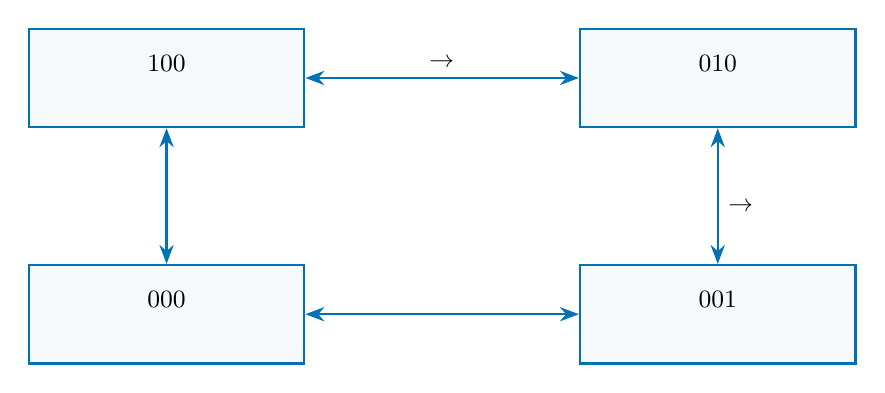
\begin{tikzpicture}[x=1cm,y=1cm,box/.style={draw=tolblue,fill=tolblue!4,line width=.8pt,align=center,inner sep=8pt,font=\small},bi/.style={<->,>=Stealth,line width=.85pt,draw=tolblue}]

\node[box,minimum width=3.5cm,minimum height=1.25cm] (a) at(0,3) {100\\{\cjkfont 价态有电子}};
\node[box,minimum width=3.5cm,minimum height=1.25cm] (b) at(7,3) {010\\{\cjkfont 价空穴＋缺陷电子}};
\node[box,minimum width=3.5cm,minimum height=1.25cm] (c) at(7,0) {001\\{\cjkfont 空间分离束缚对}};
\node[box,minimum width=3.5cm,minimum height=1.25cm] (d) at(0,0) {000\\{\cjkfont 电子已导出}};
\draw[bi] (a)--node[above,font=\small] {{\cjkfont 价态} $\to$ {\cjkfont 缺陷}}(b);
\draw[bi] (b)--node[right,font=\small,align=left] {{\cjkfont 缺陷}\\$\to$ {\cjkfont 传导态}}(c);
\draw[bi] (c)--node[above,font=\small] {{\cjkfont 电子导出}}(d);
\draw[bi] (d)--node[left,font=\small] {{\cjkfont 回填}}(a);
\end{tikzpicture}}
\caption{{\cjkfont 原创主循环示意。}\allowbreak{}100\allowbreak{}{\cjkfont 等数字依次为}\allowbreak{}V\nobreak{}{\cjkfont 、}\allowbreak{}D\nobreak{}{\cjkfont 、}\allowbreak{}C\allowbreak{}{\cjkfont 占据；完整模型包含其余四个构型及}\allowbreak{}12\allowbreak{}{\cjkfont 条无向边，图只突出解释所需的主循环。}\allowbreak{}}\label{fig:32}
{\footnotesize\color{SourceGray} {\cjkfont 新}\allowbreak{}3\allowbreak{}{\cjkfont 位点}\allowbreak{}8\allowbreak{}{\cjkfont 态图与状态能定义}\allowbreak{} \cite{D4}\par}
\end{figure}
\medskip
% ===== FROZEN SECTION 44 =====
\FloatBarrier
\Needspace{110pt}
\section{{\cjkfont 量子修正保留了高场率却没有消除低场瓶颈}\allowbreak{}}\label{sec:44}
% SOURCE 44-paragraph-0 4b8478e4b6fe9bf13e38a0317cfcc5536f07cfbb3f7a42a181b36affe13d083f
{\cjkfont 固定几何、内部}\allowbreak{}H\allowbreak{}{\cjkfont 各}\allowbreak{}10 \ensuremath{\mu}eV\nobreak{}{\cjkfont 、总}\allowbreak{}\ensuremath{\lambda}=\allowbreak{}0.20 eV\allowbreak{}{\cjkfont 和端点交换率各}\allowbreak{}10\textsuperscript{6} s\textsuperscript{−1}\nobreak{}{\cjkfont ，主扫描比较经典与有限温度量子核。}\allowbreak{}80 K\nobreak{}{\cjkfont 、}\allowbreak{}0.5 MV/cm\nobreak{}{\cjkfont ，量子净循环仅约}\allowbreak{}1.92\ensuremath{\times}10\textsuperscript{−20} s\textsuperscript{−1}\nobreak{}{\cjkfont ；到}\allowbreak{}1.5 MV/cm\allowbreak{}{\cjkfont 为}\allowbreak{}5.00\ensuremath{\times}10\textsuperscript{5} s\textsuperscript{−1}\nobreak{}{\cjkfont ；}\allowbreak{}3 MV/cm\allowbreak{}{\cjkfont 仍为}\allowbreak{}3294.9 s\textsuperscript{−1}\nobreak{}{\cjkfont ，而经典核在该强驱动点回落到}\allowbreak{}4.30\ensuremath{\times}10\textsuperscript{−36} s\textsuperscript{−1}\nobreak{}{\cjkfont 。}\allowbreak{}
\par
% SOURCE 44-paragraph-1 e051e4e80a6c4302ed66f3a71a9ac7f8777273f844dda4b771404712fc14c2ed
{\cjkfont 这说明完整占据、库仑及复位并未抹去量子核与经典核的巨大差别。但量子核不是处处更快：在}\allowbreak{}1 MV/cm\allowbreak{}{\cjkfont 的若干点反而略慢。高场弱温度依赖也不能推广到全场域，低场仍可因上坡形成而变化许多数量级。}\allowbreak{}
\par
% SOURCE 44-paragraph-2 a04110dda1d2abb4fe5155a416bcdfdb8d09d252b1b30e7294b9dca19b70cdda
{\cjkfont 若额外假设独立有效图密度}\allowbreak{}10\textsuperscript{15} cm\textsuperscript{−3}\nobreak{}{\cjkfont 、}\allowbreak{}100 nm\allowbreak{}{\cjkfont 厚度与完全收集，}\allowbreak{}\ensuremath{\Gamma}=\allowbreak{}10\textsuperscript{6} s\textsuperscript{−1}\allowbreak{}{\cjkfont 本身就给约}\allowbreak{}1.602 mA/cm\textsuperscript{2}\allowbreak{}{\cjkfont 容量上限。量子主扫描的条件峰值在}\allowbreak{}80\allowbreak{}{\cjkfont 和}\allowbreak{}300 K\allowbreak{}{\cjkfont 分别约}\allowbreak{}0.822\allowbreak{}{\cjkfont 和}\allowbreak{}0.840 mA/cm\textsuperscript{2}\nobreak{}{\cjkfont ，均未到}\allowbreak{}50 mA/cm\textsuperscript{2}\nobreak{}{\cjkfont 。没有}\allowbreak{}V50\allowbreak{}{\cjkfont 就留空，不用峰位替代上翘。}\allowbreak{}
\par
% SOURCE 44-paragraph-3 34d4e714170aba5936c5c9a5135097c9e49eea2302f4d212898667b6768a5c97
{\cjkfont 此外，局部循环的内部位移仅}\allowbreak{}10 nm\nobreak{}{\cjkfont ，在}\allowbreak{}100 nm\allowbreak{}{\cjkfont 器件中只完成约十分之一的加权电荷位移；其余载流子运动还需真实输运模型。把}\allowbreak{}qNgraphdR\allowbreak{}{\cjkfont 叫作容量换算，不能省略完全收集等前提。}\allowbreak{}
\par
\begin{figure}[!htbp]
\centering
\includegraphics[width=.90\linewidth,height=.38\textheight,keepaspectratio]{figures/graph_field.pdf}
\caption{{\cjkfont 本次}\allowbreak{}10818\allowbreak{}{\cjkfont 个高精度局部稳态解。场为给定局部参数，化学驱动按声明协议设置；纵轴为每图每秒净循环，不是器件}\allowbreak{}J–V\nobreak{}{\cjkfont 。}\allowbreak{}}\label{fig:33}
{\footnotesize\color{SourceGray} {\cjkfont 固定预算量子图主扫描与}\allowbreak{}28\allowbreak{}{\cjkfont 点独立生成树核验}\allowbreak{} \cite{D4}\par}
\end{figure}
\medskip
% ===== FROZEN SECTION 45 =====
\FloatBarrier
\Needspace{110pt}
\section{{\cjkfont 端点堵塞与提取反馈可以改变结论}\allowbreak{}}\label{sec:45}
% SOURCE 45-paragraph-0 00829f1284fc4dd57464e1d25c105607db0299efd129ce8418126b2df1b2d2ff
80 K\nobreak{}{\cjkfont 、}\allowbreak{}1.5 MV/cm\allowbreak{}{\cjkfont 时，两端交换都很慢会把图堵住。若}\allowbreak{}\ensuremath{\Gamma}V=\allowbreak{}100 s\textsuperscript{−1}\allowbreak{}{\cjkfont 而}\allowbreak{}\ensuremath{\Gamma}C=\allowbreak{}10\textsuperscript{6}\nobreak{}{\cjkfont ，价端很快缺电子；反过来，传导端几乎被填满。两个极限都把净循环限制到约}\allowbreak{}100 s\textsuperscript{−1}\allowbreak{}{\cjkfont 附近，因此冻结端点满空占据不能被当作已经处理提取。}\allowbreak{}
\par
% SOURCE 45-paragraph-1 f8b84367739c222ea5089b70c073ed33b475df69acc5811a6401ff180c43f416
{\cjkfont 更细的诊断发现，提取也未必越快越好。}\allowbreak{}80 K\nobreak{}{\cjkfont 、}\allowbreak{}2 MV/cm\allowbreak{}{\cjkfont 的含库仑量子图在}\allowbreak{}\ensuremath{\Gamma}\ensuremath{\approx}\allowbreak{}5.01\ensuremath{\times}10\textsuperscript{5} s\textsuperscript{−1}\allowbreak{}{\cjkfont 达到约}\allowbreak{}73620 s\textsuperscript{−1}\nobreak{}{\cjkfont ；继续到}\allowbreak{}10\textsuperscript{10} s\textsuperscript{−1}\nobreak{}{\cjkfont ，净率降到约}\allowbreak{}50646 s\textsuperscript{−1}\nobreak{}{\cjkfont 。关闭库仑控制后，扫描内恢复单调。}\allowbreak{}
\par
% SOURCE 45-paragraph-2 c06c25e59157825e3d7965b2b9b6cc23f6661e71d7bd296fed82b1f0e8b0402e
{\cjkfont 原因是占据改变了形成步骤的电荷构型。}\allowbreak{}C\allowbreak{}{\cjkfont 已经有电子时，}\allowbreak{}V\ensuremath{\to}D\allowbreak{}{\cjkfont 的能差与}\allowbreak{}C\allowbreak{}{\cjkfont 空时不同，在该驱动力附近反而对应更快的量子或经典核；极快提取让这条有利条件支路消失。这个非单调也存在于经典核，因此不能归因于量子振动独有。}\allowbreak{}
\par
% SOURCE 45-paragraph-3 5b832d9c5990e598ecc1273c964cb12580da85e9eb39483bc4b4b1c69218053f
{\cjkfont 这并不等于应该故意让器件提取变差。慢到造成堵塞时通量仍趋近零；在真实器件中，端点积累还会反馈电势与库仑关系。局部图只揭示占据}\allowbreak{}—\allowbreak{}{\cjkfont 能量}\allowbreak{}—\allowbreak{}{\cjkfont 速率之间的闭环，尚未完成全器件优化。}\allowbreak{}
\par
\begin{figure}[!htbp]
\centering
\includegraphics[width=.90\linewidth,height=.38\textheight,keepaspectratio]{figures/graph_feedback.pdf}
\caption{{\cjkfont 新库仑开关控制：其它内部参数固定，仅扫描端点交换。关闭相互作用是机制诊断，不是对目标材料的拟合方案。}\allowbreak{}}\label{fig:34}
{\footnotesize\color{SourceGray} {\cjkfont 端点堵塞、构型分支与提取非单调}\allowbreak{} \cite{D4}\par}
\end{figure}
\medskip
% ===== FROZEN SECTION 46 =====
\FloatBarrier
\Needspace{110pt}
\section{{\cjkfont 常数储库速率隐藏了哪些能谱假设}\allowbreak{}}\label{sec:46}
% SOURCE 46-paragraph-0 6fdc7dc897575636bf8664a25a0a1c9623083c6eeccd9002b2c97722f8ac0d73
{\cjkfont 常}\allowbreak{}\ensuremath{\Gamma}f\allowbreak{}{\cjkfont 与}\allowbreak{}\ensuremath{\Gamma}(1−f)\allowbreak{}{\cjkfont 可以完全满足详细平衡，却没有告诉我们附近真实宿主有没有可交换的电子态，以及交换是否需要吸收声子。为隔离这个问题，新阶段保持同一}\allowbreak{}8\allowbreak{}{\cjkfont 态骨架、内部耦合和重组核，给价库与传导库各一个宽}\allowbreak{}1 eV\nobreak{}{\cjkfont 、积分为}\allowbreak{}1\allowbreak{}{\cjkfont 的单侧能谱。}\allowbreak{}
\par
% SOURCE 46-paragraph-1 57f905d4cfccc4c3c357ca8f4e71374cdced6f10ff8f7cfb7b94e8bdaed4a078
{\cjkfont 价谱只在}\allowbreak{}EV\allowbreak{}{\cjkfont 以下，传导谱只在}\allowbreak{}EC\allowbreak{}{\cjkfont 以上。向端点加入一个电子的图能差为}\allowbreak{}a\nobreak{}{\cjkfont ，储库实际电子能量为}\allowbreak{}\ensuremath{\varepsilon}\nobreak{}{\cjkfont 。正向积分必须乘}\allowbreak{}f(\ensuremath{\varepsilon})\nobreak{}{\cjkfont ，反向出射必须乘}\allowbreak{}1−f(\ensuremath{\varepsilon})\nobreak{}{\cjkfont ；同一可逆核处理}\allowbreak{}a−\ensuremath{\varepsilon}\allowbreak{}{\cjkfont 和}\allowbreak{}\ensuremath{\varepsilon}−a\nobreak{}{\cjkfont 。逐能量的两个比值相乘后}\allowbreak{}\ensuremath{\varepsilon}\allowbreak{}{\cjkfont 消去，所以积分仍满足正确的热力学比。}\allowbreak{}
\par
% SOURCE 46-paragraph-2 d4b6b213eb924f9cdfe1cdf5c1041025166eeb8530d30926c369f8d5e05d3729
{\cjkfont 按}\allowbreak{}2\ensuremath{\pi}H\ensuremath{\alpha}\textsuperscript{2}/(\ensuremath{\hbar}W)=\allowbreak{}10\textsuperscript{6} s\textsuperscript{−1}\allowbreak{}{\cjkfont 匹配旧交换强度，得到}\allowbreak{}H\ensuremath{\alpha}\allowbreak{}{\cjkfont 约}\allowbreak{}10.235 \ensuremath{\mu}eV\nobreak{}{\cjkfont 。这是谱强度与单位匹配，没有用目标电流调参数。但新}\allowbreak{}\ensuremath{\Gamma}eff=\allowbreak{}k\allowbreak{}{\cjkfont 加}\allowbreak{}+k\allowbreak{}{\cjkfont 减会随构型、温度和谱支持域变化，不再是已知常数。}\allowbreak{}
\par
% SOURCE 46-paragraph-3 a7171e540b80c095d5d883c46d2dff0a5b772102b72572966c6a985dc568c37c
80 K\nobreak{}{\cjkfont 、}\allowbreak{}1.5 MV/cm\allowbreak{}{\cjkfont 的量子循环从常}\allowbreak{}\ensuremath{\Gamma}\allowbreak{}{\cjkfont 的}\allowbreak{}500482 s\textsuperscript{−1}\allowbreak{}{\cjkfont 降为单侧谱}\allowbreak{}188.638 s\textsuperscript{−1}\nobreak{}{\cjkfont ；同预算的对称宽谱允许原带隙侧态后，又回到}\allowbreak{}483197 s\textsuperscript{−1}\nobreak{}{\cjkfont 。区别来自可用交换能量，并非详细平衡突然失效。}\allowbreak{}
\par
\begin{equation}
k_+(a)=\int \rho(\epsilon)K(a-\epsilon)f(\epsilon)\,d\epsilon
\label{eq:51}\end{equation}
\begin{equation}
k_-(a)=\int \rho(\epsilon)K(\epsilon-a)[1-f(\epsilon)]\,d\epsilon
\label{eq:52}\end{equation}
\begin{equation}
\frac{k_+}{k_-}=e^{-(a-\mu)/(k_BT)}
\label{eq:53}\end{equation}
\begin{figure}[!htbp]
\centering
\includegraphics[width=.90\linewidth,height=.38\textheight,keepaspectratio]{figures/reservoir_support.pdf}
\caption{{\cjkfont 新有限带谱控制：相同内部图、归一谱权重和匹配耦合。对称宽谱包含单侧宿主带中没有的态，不能称为同一材料带结构。}\allowbreak{}}\label{fig:35}
{\footnotesize\color{SourceGray} 21636\allowbreak{}{\cjkfont 点有限谱交换重算与独立求积}\allowbreak{} \cite{D6}\par}
\end{figure}
\medskip
% ===== FROZEN SECTION 47 =====
\FloatBarrier
\Needspace{110pt}
\section{{\cjkfont 束缚对复位成为新的慢步骤}\allowbreak{}}\label{sec:47}
% SOURCE 47-paragraph-0 61f029374b1a517ddd3b69c0a47f545140a3fbd41a1b6c227f2e761f7b43babe
{\cjkfont 在上述单侧谱、}\allowbreak{}80 K\nobreak{}{\cjkfont 、}\allowbreak{}1.5 MV/cm\allowbreak{}{\cjkfont 点，图约}\allowbreak{}98.984\%\allowbreak{}{\cjkfont 的概率停在}\allowbreak{}001\nobreak{}{\cjkfont ，即}\allowbreak{}V\allowbreak{}{\cjkfont 处有空穴、}\allowbreak{}C\allowbreak{}{\cjkfont 处有电子，两者相隔}\allowbreak{}10 nm\nobreak{}{\cjkfont 。库仑结合能约}\allowbreak{}0.04114 eV\nobreak{}{\cjkfont 。内部}\allowbreak{}V\ensuremath{\to}D\allowbreak{}{\cjkfont 和}\allowbreak{}D\ensuremath{\to}C\allowbreak{}{\cjkfont 转移已经能达到每秒数百万次，但电子导出和空穴回填各只有约}\allowbreak{}95.287 s\textsuperscript{−1}\nobreak{}{\cjkfont 。}\allowbreak{}
\par
% SOURCE 47-paragraph-1 5deca00425f128f0015b7269a485efa8d2e3b6f55dcf279c4efbc3969937b1e7
{\cjkfont 原因可以逐步讲清：传导电子的添加能低于当地传导连续谱下边缘，导出需要吸收能量；价谱中的已有电子必须跃迁到高于价谱上边缘的图添加能，因此同样需要吸收能量。两个出口合起来控制完整循环约}\allowbreak{}188.638 s\textsuperscript{−1}\nobreak{}{\cjkfont 。量子内部逃逸再快，也不能跳过这个端点瓶颈。}\allowbreak{}
\par
% SOURCE 47-paragraph-2 27a2c314d213b1a38cf870ad558cc6dae87b473a4ed3cda7095ad75f916beff5
{\cjkfont 这个结果仍不是}\allowbreak{}D18:L8-BO\allowbreak{}{\cjkfont 上限。连续库接走粒子后，不再显式保留它与图内另一电荷的相关作用，这本身是开放浴粗粒化；真实载流子继续空间分离还可能获得更多场功。因此下一步应显式加入进一步分离和回填状态，同时保持总跨度与总耦合预算，不能把终端库移远却不支付重叠衰减。}\allowbreak{}
\par
% SOURCE 47-paragraph-3 775f1ff01afdd1c8bc2a16a01bf2abc746ce97913ef65fd1bd193a8f17ec98fa
{\cjkfont 同一模型还允许声子浴局部吸热。}\allowbreak{}80 K\nobreak{}{\cjkfont 、}\allowbreak{}0.5 MV/cm\allowbreak{}{\cjkfont 每净循环声子热约}\allowbreak{}−0.815 eV\nobreak{}{\cjkfont ，电子库热约}\allowbreak{}+1.315 eV\nobreak{}{\cjkfont ，总热仍为}\allowbreak{}+0.5 eV\allowbreak{}{\cjkfont 外部化学功。只看声子一项就判断违反第二定律，会漏掉电子库能量。}\allowbreak{}
\par
\begin{figure}[!htbp]
\centering
\includegraphics[width=.90\linewidth,height=.38\textheight,keepaspectratio]{figures/reservoir_temperature.pdf}
\caption{{\cjkfont 新有限谱结果：束缚对占据与完整循环温度依赖。固定探索参数下的容量峰不是材料击穿阈值。}\allowbreak{}}\label{fig:36}
{\footnotesize\color{SourceGray} {\cjkfont 束缚对态概率、逐边率及物理热分配}\allowbreak{} \cite{D6}\par}
\end{figure}
\medskip
% ===== FROZEN SECTION 48 =====
\FloatBarrier
\Needspace{110pt}
\section{{\cjkfont 固定化学势与固定载流子数不是同一温扫}\allowbreak{}}\label{sec:48}
% SOURCE 48-paragraph-0 38ef70af0f54ae58757cdeca712178138511ebb7359279a7aea3dc6581c9cd9a
{\cjkfont 为了避免符号混淆，这里把化学势写为}\allowbreak{}\ensuremath{\mu}ch\nobreak{}{\cjkfont ，迁移率写为}\allowbreak{}\ensuremath{\mu}mob\nobreak{}{\cjkfont 。若}\allowbreak{}DOS\allowbreak{}{\cjkfont 给定，载流子浓度由费米积分决定。固定}\allowbreak{}\ensuremath{\mu}ch\allowbreak{}{\cjkfont 时，冷却通常改变}\allowbreak{}n\nobreak{}{\cjkfont ；固定}\allowbreak{}n\allowbreak{}{\cjkfont 时，则必须反求}\allowbreak{}\ensuremath{\mu}ch(T)\nobreak{}{\cjkfont 。实际有偏器件还由接触、空间电荷和复合联合决定，不能无说明地把二者同时固定。}\allowbreak{}
\par
% SOURCE 48-paragraph-1 06d52d8fd043664c0dc289897c77a927d62026db47a15cfc4c29aea9269baea3
{\cjkfont 取同材料文献输运}\allowbreak{}DOS\allowbreak{}{\cjkfont 宽度}\allowbreak{}66.8 meV\allowbreak{}{\cjkfont 作为数学场景，在}\allowbreak{}300 K\allowbreak{}{\cjkfont 令}\allowbreak{}n/N=\allowbreak{}10\textsuperscript{−4}\nobreak{}{\cjkfont ，可得}\allowbreak{}\ensuremath{\mu}ch−E0\ensuremath{\approx}\allowbreak{}−0.32356 eV\nobreak{}{\cjkfont 。冷到}\allowbreak{}80 K\nobreak{}{\cjkfont ，固定该}\allowbreak{}\ensuremath{\mu}ch\allowbreak{}{\cjkfont 时费米积分给}\allowbreak{}n/N\ensuremath{\approx}\allowbreak{}9.916\ensuremath{\times}10\textsuperscript{−7}\nobreak{}{\cjkfont ；若坚持}\allowbreak{}n/N=\allowbreak{}10\textsuperscript{−4}\nobreak{}{\cjkfont ，化学势需移到约}\allowbreak{}−0.25291 eV\nobreak{}{\cjkfont 。两种计算回答的是不同问题。}\allowbreak{}
\par
% SOURCE 48-paragraph-2 5f3dbee316274ed5064aa39080d6a9f3a7c1de2e0b5ac56459736d758972b360
{\cjkfont 更严重的反例是把整个无限高斯尾都当作稀占据，盲用}\allowbreak{}Boltzmann\allowbreak{}{\cjkfont 积分，会在}\allowbreak{}80 K\allowbreak{}{\cjkfont 给}\allowbreak{}n/N\ensuremath{\approx}\allowbreak{}1.0114\nobreak{}{\cjkfont ，超过总态容量。这不是材料突然产生很多电子，而是非简并近似失效。真实低温}\allowbreak{}DOS\allowbreak{}{\cjkfont 还可能有有限宽度、库仑关联与非平衡冻结。}\allowbreak{}
\par
% SOURCE 48-paragraph-3 94d577e29f1bca7843595fd0b8210712907a80932bdf57fbfae6e5aeb6e4ad78
{\cjkfont 同理，锐带边的}\allowbreak{}ni\allowbreak{}{\cjkfont 公式只有在相应态数与稀占据假设下成立。不能把无机抛物带}\allowbreak{}Nc\ensuremath{\propto}T\textsuperscript{3⁄2}\allowbreak{}{\cjkfont 或固定分子态数两种不同图像随意混用，更不能只改}\allowbreak{}temperature\allowbreak{}{\cjkfont 而把其它发射、俘获关系留在室温定义。}\allowbreak{}
\par
\begin{equation}
n(T,\mu_{\mathrm{ch}})=\int g(E)\frac{dE}{1+e^{(E-\mu_{\mathrm{ch}})/(k_BT)}}
\label{eq:54}\end{equation}
\begin{figure}[!htbp]
\centering
\includegraphics[width=.90\linewidth,height=.38\textheight,keepaspectratio]{figures/dos_extract.pdf}
\caption{{\cjkfont 本次}\allowbreak{}DOS\allowbreak{}{\cjkfont 与提取审计。高斯宽度是文献场景，激活迁移率为探索假设；固定}\allowbreak{}\ensuremath{\mu}\allowbreak{}{\cjkfont 与固定}\allowbreak{}n\allowbreak{}{\cjkfont 是不同边界约束。}\allowbreak{}}\label{fig:37}
{\footnotesize\color{SourceGray} {\cjkfont 费米容量反例和输入范围}\allowbreak{} \cite{D3}\nobreak{}{\cjkfont ；同材料}\allowbreak{}IS\allowbreak{}{\cjkfont 宽度来源}\allowbreak{} \cite{R17}\par}
\end{figure}
\medskip
% ===== FROZEN SECTION 49 =====
\FloatBarrier
\Needspace{110pt}
\section{{\cjkfont 源产生得快还要把电荷运到电极}\allowbreak{}}\label{sec:49}
% SOURCE 49-paragraph-0 3ea01d4a0ba5534d2d7ac9942fcf4af0bccaf5f7abe2a9a4bb5a94a919549bf7
{\cjkfont 微观源率足够大，并不意味着器件端口能够收集同样电流。简单均匀漂移估计给}\allowbreak{}\ensuremath{\tau}tr\ensuremath{\approx}\allowbreak{}d/(\ensuremath{\mu}mobF)\nobreak{}{\cjkfont ，而支持某个电流需要}\allowbreak{}n\ensuremath{\approx}\allowbreak{}\ensuremath{\vert}J\ensuremath{\vert}/(q\ensuremath{\mu}mobF)\nobreak{}{\cjkfont 。冷却后若}\allowbreak{}\ensuremath{\mu}\allowbreak{}{\cjkfont 显著下降，提取时间可能比局部反应慢许多，并引起占据、复合及空间电荷反馈。}\allowbreak{}
\par
% SOURCE 49-paragraph-1 dafc0383c3bb3ebbc636669f023459999a9f47c3a8f306ee27ffdabff49e2be4
{\cjkfont 量级压力测试取}\allowbreak{}\ensuremath{\mu}300\allowbreak{}{\cjkfont 为}\allowbreak{}FF78\allowbreak{}{\cjkfont 值，迁移激活能}\allowbreak{}0.10 eV\nobreak{}{\cjkfont 、}\allowbreak{}F=\allowbreak{}1 MV/cm\nobreak{}{\cjkfont 。}\allowbreak{}300 K\allowbreak{}{\cjkfont 的渡越约}\allowbreak{}2.21 ns\nobreak{}{\cjkfont ，}\allowbreak{}80 K\allowbreak{}{\cjkfont 约}\allowbreak{}92.1 \ensuremath{\mu}s\nobreak{}{\cjkfont 。要支持}\allowbreak{}50 mA/cm\textsuperscript{2}\nobreak{}{\cjkfont ，估算}\allowbreak{}n\allowbreak{}{\cjkfont 从}\allowbreak{}6.90\ensuremath{\times}10\textsuperscript{13}\allowbreak{}{\cjkfont 增到}\allowbreak{}2.87\ensuremath{\times}10\textsuperscript{18} cm\textsuperscript{−3}\nobreak{}{\cjkfont 。相应单极空间电荷量级}\allowbreak{}qnd/(\ensuremath{\varepsilon}F)\allowbreak{}{\cjkfont 从}\allowbreak{}3.57\ensuremath{\times}10\textsuperscript{−4}\allowbreak{}{\cjkfont 增到}\allowbreak{}14.9\nobreak{}{\cjkfont ，提醒固定场和稀密度假设可能同时失效。}\allowbreak{}
\par
\begin{figure}[!htbp]
\centering
\resizebox{.90\linewidth}{!}{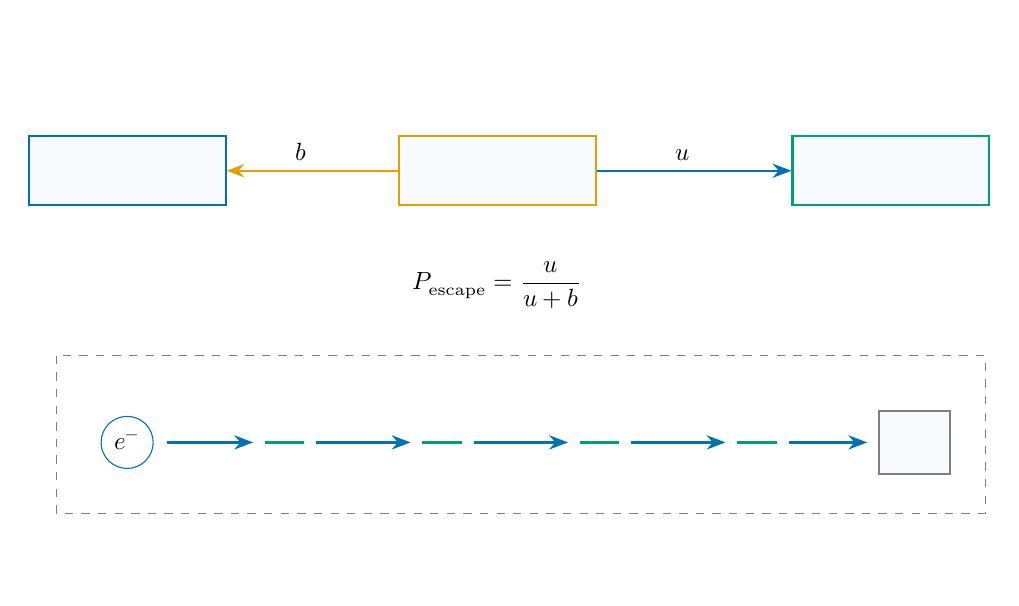
\begin{tikzpicture}[x=1cm,y=1cm,font=\small,
box/.style={draw=tolblue,line width=.75pt,fill=tolblue!3,align=center,inner sep=7pt},
arr/.style={-{Stealth},line width=.85pt,draw=tolblue},
rev/.style={-{Stealth},line width=.75pt,draw=tolorange},
both/.style={<->,>=Stealth,line width=.8pt,draw=tolblue}]

\node[font=\bfseries]at(6,3.7){{\cjkfont 局部离开成功，与到达电极，是两层问题}};
\node[box,minimum width=2.5cm](origin)at(1,2.0){{\cjkfont 返回母态}\\{\cjkfont 或原束缚态}};
\node[box,draw=tolorange,minimum width=2.5cm](near)at(5.7,2.0){{\cjkfont 刚形成的近态}\\{\cjkfont 从这里开始竞争}};
\node[box,draw=tolgreen,minimum width=2.5cm](away)at(10.7,2.0){{\cjkfont 继续分离}\\{\cjkfont 尚未到电极}};
\draw[rev](near)--node[above]{$b$ {\cjkfont 回跳}}(origin);
\draw[arr](near)--node[above]{$u$ {\cjkfont 离开}}(away);
\node at(5.7,.55){$P_{\rm escape}=\dfrac{u}{u+b}$};
\draw[gray,dashed](.1,-.35)rectangle(11.9,-2.35);
\node at(6,-.68){{\cjkfont 后续还要经过器件输运与收集}};
\node[draw=tolblue,circle,inner sep=3pt](e)at(1,-1.45){$e^-$};
\foreach \xx in {3,5,7,9}{\draw[tolgreen,line width=1pt](\xx-.25,-1.45)--(\xx+.25,-1.45);}
\draw[arr](1.5,-1.45)--(2.6,-1.45);\draw[arr](3.4,-1.45)--(4.6,-1.45);\draw[arr](5.4,-1.45)--(6.6,-1.45);\draw[arr](7.4,-1.45)--(8.6,-1.45);\draw[arr](9.4,-1.45)--(10.4,-1.45);
\node[box,draw=gray,minimum width=.9cm,minimum height=.8cm]at(11,-1.45){{\cjkfont 电极}};
\node at(6,-3.05){{\cjkfont 输运时间、再次复合、接触与空间电荷都可能改变收集}};
\end{tikzpicture}}
\caption{{\cjkfont 上排从已经形成的近态开始，只在两个恒定、互斥的指数等待出口}\allowbreak{}u\allowbreak{}{\cjkfont 和}\allowbreak{}b\allowbreak{}{\cjkfont 这一简化条件下，先成功离开的概率为}\allowbreak{}u/(u+b)\nobreak{}{\cjkfont 。箭头表示状态转移；离开这个近态不等于已被电极提取，也不排除更远处继续回跳。下排短线与箭头表示后续输运示意，没有假定固定跳数、能量阶梯或单向真实网络。最终端口电流仍需与占据、复合和自洽输运一起计算。}\allowbreak{}}\label{fig:38}
{\footnotesize\color{SourceGray} {\cjkfont 探索}\allowbreak{}E\ensuremath{\mu}=\allowbreak{}0.10 eV\nobreak{}{\cjkfont ，不是}\allowbreak{}D18\allowbreak{}{\cjkfont 低温拟合；计算与边界}\allowbreak{} \cite{D3}\par}
\end{figure}
% SOURCE 49-paragraph-2 fd332e3991378f1a9c2ee840c0e6f92b1fa26a1982c9bcfa5ae81af58bb0f9c8
{\cjkfont 这些不是新}\allowbreak{}DD\allowbreak{}{\cjkfont 解。电子和空穴的局部抵消、真实低温}\allowbreak{}\ensuremath{\mu}(T,F,n)\nobreak{}{\cjkfont 、接触与陷阱都会改变估计。它们的作用是阻止我们在量子核中得到较快速率后，立刻假定全器件完全收集。}\allowbreak{}
\par
% SOURCE 49-paragraph-3 5d89e4cfce9437dd8beec5eb44dec5e10a9e1191fb2a6c21ddb2e29c8722acfa
{\cjkfont 在最小近态竞争中，提取概率为}\allowbreak{}u/(u+b)\nobreak{}{\cjkfont ，}\allowbreak{}u\allowbreak{}{\cjkfont 为继续离开速率、}\allowbreak{}b\allowbreak{}{\cjkfont 为返回率。这个因子展示了回跳的重要性；完整多态网络则需一起求占据。未来接入}\allowbreak{}DD\allowbreak{}{\cjkfont 时，局部图净源、图电荷与全部跳跃电流必须同时反馈。}\allowbreak{}
\par
\begin{equation}
\tau_{\mathrm{tr}}\simeq\frac{d}{\mu_{\mathrm{mob}}F},\qquad n\simeq\frac{|J|}{q\mu_{\mathrm{mob}}F},\qquad \chi_{\mathrm{sc}}=\frac{qnd}{\varepsilon F}
\label{eq:55}\end{equation}
\begin{equation}
P_{\mathrm{escape}}=\frac{u}{u+b}
\label{eq:56}\end{equation}
\begin{center}\begin{minipage}{\linewidth}\small
\setlength{\TableWidth}{\dimexpr\linewidth-4\tabcolsep\relax}
\begin{tabular}{@{}>{\raggedright\arraybackslash}p{0.300\TableWidth}>{\raggedright\arraybackslash}p{0.320\TableWidth}>{\raggedright\arraybackslash}p{0.380\TableWidth}@{}}
\toprule
\bfseries {\cjkfont 量级测试}\allowbreak{} & \bfseries 300 K & \bfseries 80 K\\\midrule
\ensuremath{\mu}mob  cm\textsuperscript{2}/Vs & 4.52\ensuremath{\times}10\textsuperscript{−3} & 1.09\ensuremath{\times}10\textsuperscript{−7}\\[3pt]
{\cjkfont 渡越时间}\allowbreak{} & 2.21 ns & 92.1 \ensuremath{\mu}s\\[3pt]
50 mA/cm\textsuperscript{2}\allowbreak{}{\cjkfont 所需}\allowbreak{}n & 6.90\ensuremath{\times}10\textsuperscript{13} & 2.87\ensuremath{\times}10\textsuperscript{18} cm\textsuperscript{−3}\\[3pt]
{\cjkfont 单极}\allowbreak{}\ensuremath{\chi}sc & 3.57\ensuremath{\times}10\textsuperscript{−4} & 14.9\\[3pt]
\bottomrule\end{tabular}
\end{minipage}\end{center}
\medskip
% ===== FROZEN SECTION 50 =====
\clearpage
\part*{{\cjkfont 第五部分}\allowbreak{} \allowbreak{}{\cjkfont 数值可靠性与解释边界}\allowbreak{}}
\FloatBarrier
\Needspace{110pt}
\section{{\cjkfont 求解器停住为什么不能叫击穿}\allowbreak{}}\label{sec:50}
% SOURCE 50-paragraph-0 0ab4315c3a140e77e63c7111cb57d7c6b52610f2015ba840944f3bbcfdd4d37d
{\cjkfont 原}\allowbreak{}0.164/1.136 eV\allowbreak{}{\cjkfont 不对称诊断在}\allowbreak{}−8.4 V\allowbreak{}{\cjkfont 续接失败。独立检查发现稀疏}\allowbreak{}Jacobian\allowbreak{}{\cjkfont 方向导数正确，线性方程也求得足够准；真正问题是某个极低空穴浓度的}\allowbreak{}log-Newton\allowbreak{}{\cjkfont 步不断变大，触发全局阻尼，导致全部变量几乎不能移动。}\allowbreak{}
\par
% SOURCE 50-paragraph-1 07ae65682616109ca142fed7c402b99b30878dd02ee32198d5491a0d4ba79038
{\cjkfont 原初猜只在新电压立即改变右接触电势，内部还沿用旧值，额外电势跳变集中在最靠边的一格。给内部电势增加一个线性预测，保持}\allowbreak{}n\nobreak{}{\cjkfont 、}\allowbreak{}p\allowbreak{}{\cjkfont 初猜及所有物理方程不变，就能连续达到}\allowbreak{}−20 V\nobreak{}{\cjkfont 。这证明原失败至少可以是求根路径问题，不能被解释为该电压不存在稳态或发生材料损坏。}\allowbreak{}
\par
% SOURCE 50-paragraph-2 0f201c6542fcbf9e6b14c7aa478408aa9d549c523931571fd161ebfc22870933
{\cjkfont 这里的}\allowbreak{}Newton\allowbreak{}{\cjkfont 迭代编号不是物理时间。一个发散迭代不能当作电流随真实时间失控；相反，找到一个稳态代数根，也不证明它对真实时间扰动稳定。动态稳定需要时域方程或线性化谱，热稳定还要相应的能量方程。}\allowbreak{}
\par
% SOURCE 50-paragraph-3 bedf7147e90d6d3fb5392f19900930262bd6fb0b0d016e826ef10a54a6b821dd
{\cjkfont 本次修复没有改变势垒、密度或耦合来迎合电流。它先修初猜，再区分输出精度问题；这比把步长减小后仍失败的区间简单画成断崖更有物理意义。}\allowbreak{}
\par
\begin{equation}
\psi_{\mathrm{guess,new}}(x)=\psi_{\mathrm{old}}(x)-\frac{\Delta V}{V_T}\frac{x}{d},\qquad\psi=\frac{\phi}{V_T}
\label{eq:57}\end{equation}
\begin{figure}[!htbp]
\centering
\includegraphics[width=.90\linewidth,height=.38\textheight,keepaspectratio]{figures/newton_failure.pdf}
\caption{{\cjkfont 真实数值失败轨迹：横轴是代数}\allowbreak{}Newton\allowbreak{}{\cjkfont 迭代，不是实验时间。线性电势预测恢复同一方程的解分支。}\allowbreak{}}\label{fig:39}
{\footnotesize\color{SourceGray} {\cjkfont 独立}\allowbreak{}Jacobian\nobreak{}{\cjkfont 、阻尼和四种失败控制}\allowbreak{} \cite{D2}\par}
\end{figure}
\medskip
% ===== FROZEN SECTION 51 =====
\FloatBarrier
\Needspace{110pt}
\section{{\cjkfont 准费米变量与物理预算修复微小电流}\allowbreak{}}\label{sec:51}
% SOURCE 51-paragraph-0 4d18eef45019da673cdbeef04ac6e53694827fc9fb4d72cdf0c09a3613b87305
{\cjkfont 在另一个}\allowbreak{}−5 V\allowbreak{}{\cjkfont 误通过状态，原行缩放残差已小于阈值，但端口电流约}\allowbreak{}−7.81\ensuremath{\times}10\textsuperscript{−12} A/cm\textsuperscript{2}\nobreak{}{\cjkfont ，独立对源只有}\allowbreak{}4.90\ensuremath{\times}10\textsuperscript{−14} A/cm\textsuperscript{2}\nobreak{}{\cjkfont 。接触}\allowbreak{}SG\allowbreak{}{\cjkfont 电流实际上是约}\allowbreak{}33.7 A/cm\textsuperscript{2}\allowbreak{}{\cjkfont 的两个大项相减；几个浮点数中的微小电化学势差已被舍入。}\allowbreak{}
\par
% SOURCE 51-paragraph-1 bc6fd1adefd25c72221e6840619e46cd07bebeab186dca29633022230e4a936d
{\cjkfont 这里}\allowbreak{}VT=\allowbreak{}kBT/q\nobreak{}{\cjkfont 、}\allowbreak{}h=\allowbreak{}\ensuremath{\Delta}x/d\nobreak{}{\cjkfont 、}\allowbreak{}n0=\allowbreak{}\ensuremath{\varepsilon}VT/(qd\textsuperscript{2})\nobreak{}{\cjkfont 、}\allowbreak{}j0=\allowbreak{}q\ensuremath{\mu}nVTn0/d\nobreak{}{\cjkfont 。令}\allowbreak{}ln(n/n0)=\allowbreak{}ln(nM/n0)+\ensuremath{\psi}−\ensuremath{\psi}R+u\nobreak{}{\cjkfont ，}\allowbreak{}ln(p/n0)=\allowbreak{}ln(pM/n0)−\ensuremath{\psi}+v\nobreak{}{\cjkfont ，}\allowbreak{}nM\nobreak{}{\cjkfont 、}\allowbreak{}pM\allowbreak{}{\cjkfont 为相应多数接触浓度。采用这些准费米变量，再利用}\allowbreak{}Bernoulli\allowbreak{}{\cjkfont 函数}\allowbreak{}B(−z)=\allowbreak{}exp(z)B(z)\nobreak{}{\cjkfont ，可把电流写成}\allowbreak{}expm1(\ensuremath{\Delta}u)\nobreak{}{\cjkfont 、}\allowbreak{}expm1(\ensuremath{\Delta}v)\allowbreak{}{\cjkfont 形式。}\allowbreak{}expm1\allowbreak{}{\cjkfont 在小自变量时直接计算}\allowbreak{}exp(z)−1\nobreak{}{\cjkfont ，避免先得到两个接近}\allowbreak{}1\allowbreak{}{\cjkfont 的数再相减。但若}\allowbreak{}\ensuremath{\Delta}u\allowbreak{}{\cjkfont 仍从已经舍入的旧}\allowbreak{}log\allowbreak{}{\cjkfont 密度重建，丢失的信息不能恢复，所以必须把}\allowbreak{}u\nobreak{}{\cjkfont 、}\allowbreak{}v\allowbreak{}{\cjkfont 作为权威求解状态。}\allowbreak{}
\par
% SOURCE 51-paragraph-2 fb9ccd240d86f357810caef4f61bfbbce93e6cbee9e84bea1e174e578d20e6e0
{\cjkfont 加上独立源积分与端口电流预算后，原误通过状态再做一次}\allowbreak{}Newton\allowbreak{}{\cjkfont 即可把物理误差从约}\allowbreak{}1.53\ensuremath{\times}10\textsuperscript{−11}\allowbreak{}{\cjkfont 降到}\allowbreak{}4.73\ensuremath{\times}10\textsuperscript{−21} A/cm\textsuperscript{2}\nobreak{}{\cjkfont 。}\allowbreak{}90\allowbreak{}{\cjkfont 位原始}\allowbreak{}SG\allowbreak{}{\cjkfont 表达式在同一准费米状态上给出一致结果；将旧舍入状态改用高精度再算则无济于事。}\allowbreak{}
\par
% SOURCE 51-paragraph-3 f23bd13f6155273c027ace5c59e269c9f36bfa14c968dd446b3d3342b40fa300
{\cjkfont 对称}\allowbreak{}−20 V\allowbreak{}{\cjkfont 高电流新旧实现相差约}\allowbreak{}6.11\ensuremath{\times}10\textsuperscript{−16} A/cm\textsuperscript{2}\nobreak{}{\cjkfont ，说明修复没有抹去原}\allowbreak{}180 mA/cm\textsuperscript{2}\allowbreak{}{\cjkfont 结果。物理正确性仍需另审，网格误差也仍约}\allowbreak{}0.4\%\nobreak{}{\cjkfont 。}\allowbreak{}
\par
\begin{equation}
J_n=\frac{j_0}{h}\frac{n_L}{n_0}B(-\Delta\psi)\,\mathrm{expm1}(\Delta u)
\label{eq:58}\end{equation}
\begin{equation}
J_p=-\frac{j_0}{h}\frac{\mu_p}{\mu_n}\frac{p_L}{n_0}B(\Delta\psi)\,\mathrm{expm1}(\Delta v)
\label{eq:59}\end{equation}
\begin{figure}[!htbp]
\centering
\includegraphics[width=.90\linewidth,height=.38\textheight,keepaspectratio]{figures/qf_recovery.pdf}
\caption{{\cjkfont 新数值表示与独立预算。稳定求根、可观测电流精度和空间网格收敛是三个不同层次，不能互相替代。}\allowbreak{}}\label{fig:40}
{\footnotesize\color{SourceGray} 90\allowbreak{}{\cjkfont 位原}\allowbreak{}SG\allowbreak{}{\cjkfont 核验、对称回归及恢复曲线}\allowbreak{} \cite{D2}\nobreak{}{\cjkfont ；低温循环源扩展}\allowbreak{} \cite{D7}\par}
\end{figure}
\medskip
% ===== FROZEN SECTION 52 =====
\FloatBarrier
\Needspace{110pt}
\section{{\cjkfont 低温会把浮点相消伪装成产生通道}\allowbreak{}}\label{sec:52}
% SOURCE 52-paragraph-0 590a7ea607c3ff31bf38189881778ff086ffa19110eb9103acf110a68dfb96f1
{\cjkfont 新低温率审计发现，即使采用稳定准费米电流，反应源本身的大项相减仍可失败。}\allowbreak{}80 K\nobreak{}{\cjkfont 、}\allowbreak{}Dn/Dp=\allowbreak{}0.164/1.136 eV\nobreak{}{\cjkfont 、}\allowbreak{}−5 V\allowbreak{}{\cjkfont 时，旧计算给端流约}\allowbreak{}−1.09\ensuremath{\times}10\textsuperscript{−30} A/cm\textsuperscript{2}\nobreak{}{\cjkfont ，独立完整对源却只有}\allowbreak{}3.37\ensuremath{\times}10\textsuperscript{−52} A/cm\textsuperscript{2}\nobreak{}{\cjkfont ，端流与对源之比约}\allowbreak{}3.22\ensuremath{\times}10\textsuperscript{21}\nobreak{}{\cjkfont ；旧电子净源}\allowbreak{}2.17\ensuremath{\times}10\textsuperscript{−30}\allowbreak{}{\cjkfont 与对源之比才是}\allowbreak{}6.45\ensuremath{\times}10\textsuperscript{21}\nobreak{}{\cjkfont 。这里没有率下溢；假源来自捕获与发射的舍入相消。}\allowbreak{}
\par
% SOURCE 52-paragraph-1 27ec8e14bc8d796c008eba05e74f100ca2fddd8c6f510b692c250ef09b14a7a6
150 K\allowbreak{}{\cjkfont 同点误差仍约}\allowbreak{}5.6\allowbreak{}{\cjkfont 万倍，到}\allowbreak{}220 K\allowbreak{}{\cjkfont 约}\allowbreak{}0.218\%\nobreak{}{\cjkfont 。这说明“绝对误差非常小”不能用来证明一个更小的净信号可靠。极微平均率本来只是数学压力测试，更不能因曲线平滑就当作可测低温电流。}\allowbreak{}
\par
% SOURCE 52-paragraph-2 5f99dcf42fd699e7362d855463e7db8812fd2fbc3593dfe2b7a61c15028fee1c
{\cjkfont 修复保持相同物理率，用完整循环的正反乘积及}\allowbreak{}expm1\allowbreak{}{\cjkfont 稳定表达式构造净源，并加独立相对物理预算。新双精度积分总源与}\allowbreak{}110\allowbreak{}{\cjkfont 位逐事件相减相对差不超过}\allowbreak{}1.85\ensuremath{\times}10\textsuperscript{−16}\nobreak{}{\cjkfont 。}\allowbreak{}16\allowbreak{}{\cjkfont 个主网格反偏、}\allowbreak{}8\allowbreak{}{\cjkfont 个精确非零内建场平衡及}\allowbreak{}4\allowbreak{}{\cjkfont 个细网格状态接受了限定验证。}\allowbreak{}
\par
% SOURCE 52-paragraph-3 14d8e9db9eaa1802482c06ea84792e0f664122f6c81a07c0c38d2bb3d23d588c
{\cjkfont 但}\allowbreak{}80 K\allowbreak{}{\cjkfont 空间网格变化仍为}\allowbreak{}0.4–0.7\%\nobreak{}{\cjkfont ，经典率与固定迁移率没有低温材料标定。数值修复提高的是“给定方程被算对”的可信度，没有把那组经典方程变成}\allowbreak{}77 K\allowbreak{}{\cjkfont 器件预测。}\allowbreak{}
\par
\begin{figure}[!htbp]
\centering
\includegraphics[width=.90\linewidth,height=.38\textheight,keepaspectratio]{figures/lowT_cancellation.pdf}
\caption{{\cjkfont 本次第三阶段数值重算。极微电流是形式平均率测试；数值假源被消除，不意味着对应材料过程已得到验证。}\allowbreak{}}\label{fig:41}
{\footnotesize\color{SourceGray} {\cjkfont 循环净源、}\allowbreak{}110\allowbreak{}{\cjkfont 位逐事件和相对门槛}\allowbreak{} \cite{D7}\par}
\end{figure}
\medskip
% ===== FROZEN SECTION 53 =====
\FloatBarrier
\Needspace{110pt}
\section{{\cjkfont 历史探索与本次新证据如何区分}\allowbreak{}}\label{sec:53}
% SOURCE 53-paragraph-0 be896dbdc94d38eec7f476926642ea34df55959c624b90668b9f20ca53169dc8
{\cjkfont 在持续研究中，保留失败与局限和保留成功一样重要。本次可读取的原}\allowbreak{}FF78\allowbreak{}{\cjkfont 工程保留了代码、参数和大量扫描；新的率、数值、量子及储库检查点又有独立冻结数据。它们可以支持正文明确限定的数值陈述。}\allowbreak{}
\par
% SOURCE 53-paragraph-1 5380b4632cbb8b61bdc592d23ccccf658c8b4b00d8b919a53725a1d3208e35ac
{\cjkfont 另一些更早的有限状态图、归一谱展宽和固定跨度桥探索，在工作区恢复后只留下部分图像或讨论摘要。缺失完整代码、参数和原始数值时，不能因为图看起来合理，就把它写成今天已经复现的结果。本书保留其研究问题和方法约束，不从历史图片重新提取精确阈值或测试数量。}\allowbreak{}
\par
% SOURCE 53-paragraph-2 0f5b5c8870d7b6797d1b4cb0a4840d545863bbcac4982c2dc366ece8448aa83e
{\cjkfont 归一谱展宽的可靠一般认识是：它改变可用能量分布和峰形，但在固定总耦合下仍受核上界约束。固定带边桥的可靠研究原则是：缩短每步跨度必须与能量支持、返回及预算一起比较。新}\allowbreak{}8\allowbreak{}{\cjkfont 态图和新有限带谱已重新建立这些问题的一部分，却不等于恢复了旧代码，也未完成真实空间桥的全部自洽闭合。}\allowbreak{}
\par
% SOURCE 53-paragraph-3 827b6824f81fb226d271f2018c90a4fc6cfa3a248cb12b4701e16575ab607b07
{\cjkfont 源包另保留四张确实找回的历史图及路径哈希，只供路线回顾。它们没有被混入本书重绘曲线或新统计。未来若重建这些方案，应给新的版本、参数和验证，不覆盖历史记录或让旧图冒充新结果。}\allowbreak{}
\par
\nopagebreak[4]
{\footnotesize\color{SourceGray} % SOURCE 53-refs-0 3134eb89dcb1b6c05c69d94107828fdf8beeac928f003ffd006ab6075961aaaa
{\cjkfont 历史图单独归档；正文量化结论限于}\allowbreak{}\cite{D0}–\cite{D7}\allowbreak{}{\cjkfont 中可核验的资料}\allowbreak{}\par}
\medskip
% ===== FROZEN SECTION 54 =====
\FloatBarrier
\Needspace{110pt}
\section{{\cjkfont 默认参数下的数值比较}\allowbreak{}}\label{sec:54}
% SOURCE 54-paragraph-0 526a7885faae860e0165a68dd04a7c919cd15c94cdc3e1a963606dff872f702c
{\cjkfont 下表集中列出原}\allowbreak{}FF78\allowbreak{}{\cjkfont 存档的默认比较点。厚度}\allowbreak{}100 nm\nobreak{}{\cjkfont 、环境}\allowbreak{}300 K\nobreak{}{\cjkfont 、规定光生尺度}\allowbreak{}25 mA/cm\textsuperscript{2}\nobreak{}{\cjkfont ；电热反扫为}\allowbreak{}2 V/s\nobreak{}{\cjkfont ，其余按各自声明的稳态或缩约模型。各模型新增参数都是探索值，因此表格是条件结果，不是机制排名或实验拟合优度。}\allowbreak{}
\par
% SOURCE 54-paragraph-1 f505d51df02bca814c4dd3dfcfac42aff16fc590eab7ae520d128fb366f55d51
K50\allowbreak{}{\cjkfont 取}\allowbreak{}80\nobreak{}{\cjkfont 、}\allowbreak{}100\nobreak{}{\cjkfont 、}\allowbreak{}120 nm\allowbreak{}{\cjkfont 三点拟合，截距自由。后续}\allowbreak{}PF\allowbreak{}{\cjkfont 五厚度扫描的}\allowbreak{}0.15296 V/nm\allowbreak{}{\cjkfont 属于另一个拟合区间，不应混入这一列。模型未跨阈值时留空；电热与经验支路的小负斜率接近零，来源包含数值提取和特定不随厚度变化的构成设定，不能解释成负击穿场。}\allowbreak{}
\par
% SOURCE 54-paragraph-2 4533837fc0636d51f3e98ccc918a2598e204ffca8f3f8bdea4173e4a6e7f77e5
{\cjkfont 局域全倍率的常规}\allowbreak{}FF\allowbreak{}{\cjkfont 不适用，}\allowbreak{}A\allowbreak{}{\cjkfont 到}\allowbreak{}D\allowbreak{}{\cjkfont 详细结果已在前文说明。量子局部图没有完整器件输运和真实图密度，不应硬填}\allowbreak{}FF\allowbreak{}{\cjkfont 或}\allowbreak{}V50\allowbreak{}{\cjkfont 进入此表。真正有说服力的下一阶段比较，应使用同一组独立约束的材料参数，并预测没有参与校准的温度、厚度或接触条件。}\allowbreak{}
\par
\begin{center}\begin{minipage}{\linewidth}\small
\setlength{\TableWidth}{\dimexpr\linewidth-8\tabcolsep\relax}
\begin{tabular}{@{}>{\raggedright\arraybackslash}p{0.320\TableWidth}>{\raggedright\arraybackslash}p{0.180\TableWidth}>{\raggedright\arraybackslash}p{0.160\TableWidth}>{\raggedright\arraybackslash}p{0.170\TableWidth}>{\raggedright\arraybackslash}p{0.170\TableWidth}@{}}
\toprule
\bfseries {\cjkfont 模型}\allowbreak{} & \bfseries FF \% & \bfseries Voc V & \bfseries V50 V & \bfseries K50 V/nm\\\midrule
{\cjkfont 局域}\allowbreak{}SRH & 78.00 & 0.951 & {\cjkfont 未达到}\allowbreak{} & —\\[3pt]
{\cjkfont 有限}\allowbreak{}PF & 77.95 & 0.951 & −16.504 & 0.1581\\[3pt]
MA\allowbreak{}{\cjkfont 距离分布}\allowbreak{} & 75.48 & 0.940 & −18.724 & 0.1751\\[3pt]
{\cjkfont 有效接触}\allowbreak{} & 77.97 & 0.951 & −17.288 & 0.1727\\[3pt]
{\cjkfont 集总电热}\allowbreak{} & 77.15 & 0.942 & −11.742 & {\cjkfont 约}\allowbreak{}0\\[3pt]
{\cjkfont 局部弱区}\allowbreak{} & 76.52 & 0.950 & −17.090 & 0.1594\\[3pt]
{\cjkfont 经验支路}\allowbreak{} & 78.00 & 0.951 & −17.036 & {\cjkfont 约}\allowbreak{}0\\[3pt]
{\cjkfont 弹性}\allowbreak{}WKB\allowbreak{}{\cjkfont 微结}\allowbreak{} & 53.69 & 0.934 & −3.088 & 0.03056\\[3pt]
\bottomrule\end{tabular}
\par\vspace{6pt}{\footnotesize\color{SourceGray} {\cjkfont 原}\allowbreak{}comparison\_\allowbreak{}metrics\nobreak{}{\cjkfont 、}\allowbreak{}K50\_\allowbreak{}FF\allowbreak{}{\cjkfont 及}\allowbreak{}tat\_\allowbreak{}results\nobreak{}{\cjkfont ；均为存档条件结果}\allowbreak{} \cite{D0}\par}
\end{minipage}\end{center}
\medskip
% ===== FROZEN SECTION 55 =====
\FloatBarrier
\Needspace{110pt}
\section{{\cjkfont 一张模型成绩单需要三个独立维度}\allowbreak{}}\label{sec:55}
% SOURCE 55-paragraph-0 724d9840d1c0e060adbf62fd7d47d23178487bb269ffe2877f272cbaa7e3cc7f
{\cjkfont 这里不按“曲线像不像”给机制排座次。数学自洽、数值可靠和材料适用分别回答不同问题；一个模型可以前两项通过、第三项尚缺证据。也可以因为某个实现错误而失败，却不意味着整类物理机制被否定。}\allowbreak{}
\par
% SOURCE 55-paragraph-1 158bc894140cabe90f7f5e150576d51026860411753e0c706b0b66f30187d6ff
{\cjkfont 原有限距离}\allowbreak{}PF\allowbreak{}{\cjkfont 目前最大的优点是可以在指定方程内形成持续配对源，且完整账本被重证；最大问题是双支吸引势与远程耦合。局域全倍率的失败则更多来自该闭合同时放大复合，不能代表所有}\allowbreak{}PF\nobreak{}{\cjkfont 。量子图把状态和浴显式化后解决了一些逻辑问题，却暴露储库谱与空间分离的新问题。}\allowbreak{}
\par
% SOURCE 55-paragraph-2 4d9c98fb9f5671654523d0a9f3df7682fb9f9d663f651e28be601e15414ea900
{\cjkfont 接触、电热、弱区和经验支路说明存在竞争解释，但不同层级无法直接横比数值优劣。独立}\allowbreak{}TAT\allowbreak{}{\cjkfont 具有真实}\allowbreak{}WKB\allowbreak{}{\cjkfont 积分，却仍缺体相带边和全器件电荷反馈。任何“最终机制”都还需要同一组受约束参数对多个独立观测负责。}\allowbreak{}
\par
\begin{center}\begin{minipage}{\linewidth}\small
\setlength{\TableWidth}{\dimexpr\linewidth-4\tabcolsep\relax}
\begin{tabular}{@{}>{\raggedright\arraybackslash}p{0.300\TableWidth}>{\raggedright\arraybackslash}p{0.320\TableWidth}>{\raggedright\arraybackslash}p{0.380\TableWidth}@{}}
\toprule
\bfseries {\cjkfont 模型}\allowbreak{} & \bfseries {\cjkfont 已经得到什么}\allowbreak{} & \bfseries {\cjkfont 仍不能据此宣称}\allowbreak{}\\\midrule
{\cjkfont 局域}\allowbreak{}SRH & {\cjkfont 平衡与基线正常}\allowbreak{} & {\cjkfont 能解释反向膝点}\allowbreak{}\\[3pt]
{\cjkfont 局域}\allowbreak{}A\allowbreak{}{\cjkfont 到}\allowbreak{}D & {\cjkfont 闭合消融与瓶颈}\allowbreak{} & {\cjkfont 唯一微观}\allowbreak{}PF\allowbreak{}{\cjkfont 实现}\allowbreak{}\\[3pt]
{\cjkfont 有限距离}\allowbreak{}PF & {\cjkfont 大体源和全账本重证}\allowbreak{} & {\cjkfont 双支}\allowbreak{}PF\allowbreak{}{\cjkfont 材料依据成立}\allowbreak{}\\[3pt]
MA\allowbreak{}{\cjkfont 距离分布}\allowbreak{} & {\cjkfont 距离代价与可逆跳跃}\allowbreak{} & {\cjkfont 已测缺陷核}\allowbreak{}\\[3pt]
Marcus\allowbreak{}{\cjkfont 及量子图}\allowbreak{} & {\cjkfont 热核与占据显式化}\allowbreak{} & {\cjkfont 目标}\allowbreak{}77 K\allowbreak{}{\cjkfont 曲线}\allowbreak{}\\[3pt]
{\cjkfont 显式有限谱}\allowbreak{} & {\cjkfont 发现端点复位瓶颈}\allowbreak{} & {\cjkfont 材料电流上限}\allowbreak{}\\[3pt]
{\cjkfont 顺序}\allowbreak{}WKB\allowbreak{}{\cjkfont 微结}\allowbreak{} & {\cjkfont 弹性谱率与两端守恒}\allowbreak{} & {\cjkfont 自洽体相}\allowbreak{}TAT\\[3pt]
{\cjkfont 接触}\allowbreak{} \allowbreak{}{\cjkfont 热}\allowbreak{} \allowbreak{}{\cjkfont 弱区}\allowbreak{} & {\cjkfont 具体竞争机制例子}\allowbreak{} & {\cjkfont 已排除其它解释}\allowbreak{}\\[3pt]
{\cjkfont 经验支路}\allowbreak{} & {\cjkfont 透明曲线描述}\allowbreak{} & {\cjkfont 参数有唯一微观含义}\allowbreak{}\\[3pt]
\bottomrule\end{tabular}
\par\vspace{6pt}{\footnotesize\color{SourceGray} {\cjkfont 按本书实际完成范围汇总}\allowbreak{} \cite{D0}–\cite{D7}\par}
\end{minipage}\end{center}
\medskip
% ===== FROZEN SECTION 56 =====
\clearpage
\part*{{\cjkfont 第六部分}\allowbreak{} \allowbreak{}{\cjkfont 下一步与可检验预测}\allowbreak{}}
\FloatBarrier
\Needspace{110pt}
\section{{\cjkfont 现阶段怎样设计有边界的理论比较}\allowbreak{}}\label{sec:56}
% SOURCE 56-paragraph-0 cad2c4dd6583a8b1b077751659ef6b4cf0673063c49420dda8410a9ebcc1523e
{\cjkfont 下一步应保持同一初末端点、总跨度与总耦合预算，比较不同的形成}\allowbreak{}—\allowbreak{}{\cjkfont 转移}\allowbreak{}—\allowbreak{}{\cjkfont 继续分离}\allowbreak{}—\allowbreak{}{\cjkfont 返回}\allowbreak{}—\allowbreak{}{\cjkfont 储库导出结构。每增加一个状态，都说明它代表什么电子态、在哪里、占据多少粒子、怎样改变化学势或库仑能，避免用任意中隙阶梯免费填平跨隙代价。}\allowbreak{}
\par
% SOURCE 56-paragraph-1 fed70b7630dcd22316b85e7efed0c2d62b6cd7cbf1150dfdb41f66b61705d316
{\cjkfont 先不接器件时，局部图可输出容量、占据、返回比例、谱支持域和能量账本。再接}\allowbreak{}Poisson–\allowbreak{}{\cjkfont 输运方程时，必须同时提供净电子}\allowbreak{}/\allowbreak{}{\cjkfont 空穴源、图电荷或偶极、非局域跳跃电流，以及与局部}\allowbreak{}n\nobreak{}{\cjkfont 、}\allowbreak{}p\allowbreak{}{\cjkfont 或准费米能级一致的储库条件。只把一个正向速率作为}\allowbreak{}G(F)\allowbreak{}{\cjkfont 塞进去，会遗漏负反馈与平衡。}\allowbreak{}
\par
% SOURCE 56-paragraph-2 43443af876c09468d91743be70133a10a219912c104b9f6ba13063666a096da7
{\cjkfont 接受标准应在看曲线前确定：共同}\allowbreak{}\ensuremath{\mu}\allowbreak{}{\cjkfont 的有限场逐边零流；概率合法；循环亲和力正确；电荷和能量逐态守恒；单位与谱归一清楚；高精度与独立算法代表点一致；场}\allowbreak{}/\allowbreak{}{\cjkfont 网格}\allowbreak{}/\allowbreak{}{\cjkfont 积分范围公开；失败和未跨阈值不隐藏。}\allowbreak{}
\par
% SOURCE 56-paragraph-3 98bb17d036ba553c2cb2274e7d7f589a8da0198c6fd940ea11c9ea4be9a4efa8
{\cjkfont 当某组有材料依据的参数仍不能给出足够容量，这是一个结果。应先查瓶颈属于形成、谱、回跳还是提取，再判断需要哪一项新的微观证据，而不是依次调}\allowbreak{}\ensuremath{\lambda}\nobreak{}{\cjkfont 、}\allowbreak{}H\nobreak{}{\cjkfont 、}\allowbreak{}Nt\allowbreak{}{\cjkfont 直到上翘出现。}\allowbreak{}
\par
\begin{figure}[!htbp]
\centering
\resizebox{.90\linewidth}{!}{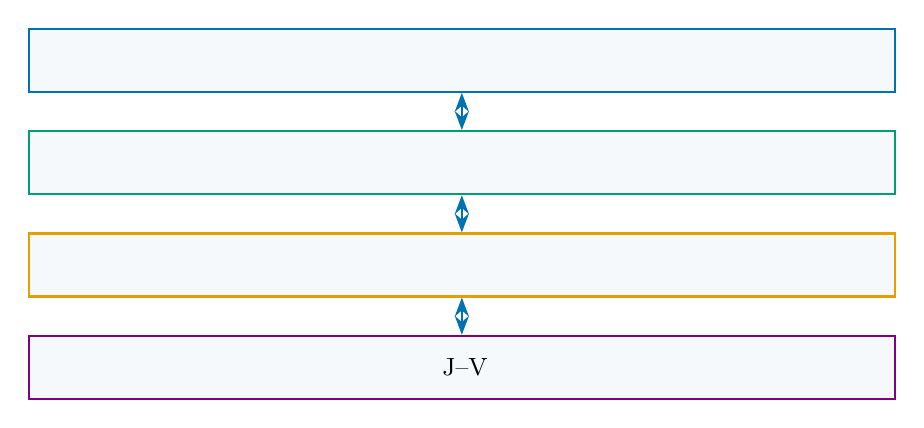
\begin{tikzpicture}[x=1cm,y=1cm,box/.style={draw=tolblue,fill=tolblue!4,line width=.8pt,align=center,inner sep=8pt,font=\small},bi/.style={<->,>=Stealth,line width=.85pt,draw=tolblue}]

\node[box,minimum width=11cm,minimum height=.8cm] (a) at(0,3.9) {{\cjkfont 微观态与热核\quad 能级 电荷 耦合 振动谱}};
\node[box,draw=tolgreen,minimum width=11cm,minimum height=.8cm] (b) at(0,2.6) {{\cjkfont 完整可逆循环\quad 形成 返回 占据 复位}};
\node[box,draw=tolorange,minimum width=11cm,minimum height=.8cm] (c) at(0,1.3) {{\cjkfont 空间器件与接触\quad 净源 电荷 场 输运}};
\node[box,draw=violet,minimum width=11cm,minimum height=.8cm] (d) at(0,0) {{\cjkfont 可观测量与实验}\quad J--V {\cjkfont 温度 厚度 时间}};
\draw[bi](a)--(b);\draw[bi](b)--(c);\draw[bi](c)--(d);
\end{tikzpicture}}
\caption{{\cjkfont 原创研究层级图。每一层向下一层传递的不只是一个电流数字，还包括占据、电荷、能量、反向过程和适用范围。}\allowbreak{}}\label{fig:42}
{\footnotesize\color{SourceGray} {\cjkfont 从可逆率到自洽器件的闭合要求}\allowbreak{} \cite{D1} \cite{D3} \cite{D4} \cite{D6}\par}
\end{figure}
\medskip
% ===== FROZEN SECTION 57 =====
\FloatBarrier
\Needspace{110pt}
\section{{\cjkfont 未来实验应该检验什么而不是先猜答案}\allowbreak{}}\label{sec:57}
% SOURCE 57-paragraph-0 a2f99e9c35ec91fb386d42b1ddb17f3978aee6b54cbafa888855a0e80f716f11
{\cjkfont 用户希望先理解理论，再开展低温实验。这条顺序合理：当前许多决定性检查并不依赖新数据。下面列的是未来能够区分候选的观测逻辑，不是要求立刻执行的仪器操作或危险高压程序。}\allowbreak{}
\par
% SOURCE 57-paragraph-1 cc90154cbb0bc3d0af805a4b771f98a059f0ab65b5165c93744cb1e2533bbb93
{\cjkfont 暗亮上翘近似重合应作为约束保留，同时比较绝对暗流、光电流差和光强依赖。只看阈值接近，既不能证明纯体源，也不能排除接触或热。必须确认同一像素、同一实际端压、相同温度与历史，而不是把不同文件标签凑成配对。}\allowbreak{}
\par
% SOURCE 57-paragraph-2 1cb24bceca43fea0b79caac9e62f0ad308d99251fe8397abdc4b167bf7abe257
{\cjkfont 温度、厚度、时间和接触应联合考虑。某高场点的弱温度依赖可以来自量子侧带、占据窗饱和或其它过程；低温电流消失也可能来自提取而非产生。热边界与脉冲长度改变可约束电热，但台温稳定并不等于活性层无局部温升。}\allowbreak{}
\par
% SOURCE 57-paragraph-3 1a3cd931d82c08c9511767eee1e2fcf278b32f95273c465586b5f28be98df715
{\cjkfont 不可逆损伤需要独立判据，例如循环前后性能、持久漏电变化或空间变化，而不是把达到}\allowbreak{}50 mA/cm\textsuperscript{2}\allowbreak{}{\cjkfont 直接叫击穿。对高场试验，仪器限流、实际波形及数据时间序列是解释的一部分，应避免越过已授权和安全的实验范围。}\allowbreak{}
\par
\begin{center}\begin{minipage}{\linewidth}\small
\setlength{\TableWidth}{\dimexpr\linewidth-2\tabcolsep\relax}
\begin{tabular}{@{}>{\raggedright\arraybackslash}p{0.360\TableWidth}>{\raggedright\arraybackslash}p{0.640\TableWidth}@{}}
\toprule
\bfseries {\cjkfont 要区分的因素}\allowbreak{} & \bfseries {\cjkfont 有信息量的联合观测}\allowbreak{}\\\midrule
{\cjkfont 体源与接触供给}\allowbreak{} & {\cjkfont 同像素暗亮幅值}\allowbreak{} \allowbreak{}{\cjkfont 接触条件}\allowbreak{} \allowbreak{}{\cjkfont 全通量账本}\allowbreak{}\\[3pt]
{\cjkfont 热}\allowbreak{}PF\allowbreak{}{\cjkfont 与量子转移}\allowbreak{} & Eapp\allowbreak{}{\cjkfont 随场变化}\allowbreak{} \allowbreak{}{\cjkfont 恢复时间}\allowbreak{} \allowbreak{}{\cjkfont 跨温区形状}\allowbreak{}\\[3pt]
{\cjkfont 产生与提取}\allowbreak{} & {\cjkfont 低温输运时间}\allowbreak{} \allowbreak{}{\cjkfont 占据或空间电荷}\allowbreak{} \allowbreak{}{\cjkfont 收集效率}\allowbreak{}\\[3pt]
{\cjkfont 恒温与电热}\allowbreak{} & {\cjkfont 相同初态下时长}\allowbreak{} \allowbreak{}{\cjkfont 扫速}\allowbreak{} \allowbreak{}{\cjkfont 散热与实际温度}\allowbreak{}\\[3pt]
{\cjkfont 均匀体与弱区}\allowbreak{} & {\cjkfont 面积统计}\allowbreak{} \allowbreak{}{\cjkfont 局部电流或热空间分布}\allowbreak{}\\[3pt]
{\cjkfont 可逆上翘与损伤}\allowbreak{} & {\cjkfont 重复循环与测前测后不可逆变化}\allowbreak{}\\[3pt]
\bottomrule\end{tabular}
\end{minipage}\end{center}
\begin{figure}[!htbp]
\centering
\resizebox{.90\linewidth}{!}{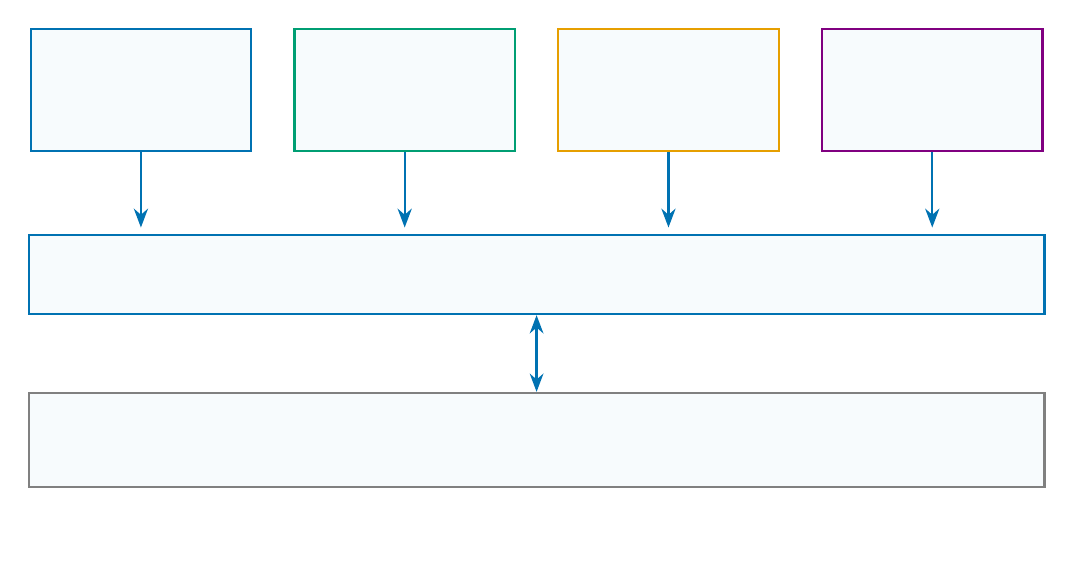
\begin{tikzpicture}[x=1cm,y=1cm,font=\small,
box/.style={draw=tolblue,line width=.75pt,fill=tolblue!3,align=center,inner sep=7pt},
arr/.style={-{Stealth},line width=.85pt,draw=tolblue},
rev/.style={-{Stealth},line width=.75pt,draw=tolorange},
both/.style={<->,>=Stealth,line width=.8pt,draw=tolblue}]

\node[box,minimum width=2.8cm,minimum height=1.55cm](a)at(0,2.7){{\cjkfont 体产对}\\{\cjkfont 形成、回填、分离}};
\node[box,draw=tolgreen,minimum width=2.8cm,minimum height=1.55cm](b)at(3.35,2.7){{\cjkfont 接触供给}\\{\cjkfont 注入、传输、提取}};
\node[box,draw=tolorange,minimum width=2.8cm,minimum height=1.55cm](c)at(6.7,2.7){{\cjkfont 电热反馈}\\{\cjkfont 功率、温升、速率}};
\node[box,draw=violet,minimum width=2.8cm,minimum height=1.55cm](d)at(10.05,2.7){{\cjkfont 空间弱区}\\{\cjkfont 局部面积、局部场}};
\node[box,minimum width=12.9cm,minimum height=1.0cm](obs)at(5.025,.35){{\cjkfont 可以产生相似的电流上翘，且机制可以共存}\\{\cjkfont 单一阈值或一段直线不足以唯一鉴定}};
\draw[arr](a.south)--(0,.95);\draw[arr](b.south)--(3.35,.95);\draw[arr](c.south)--(6.7,.95);\draw[arr](d.south)--(10.05,.95);
\node[box,draw=gray,minimum width=12.9cm,minimum height=1.2cm](tests)at(5.025,-1.75){{\cjkfont 联合观察与共同约束}\\{\cjkfont 温度＋输运时间}\quad {\cjkfont 接触＋暗亮幅值}\quad {\cjkfont 时长＋散热}\quad {\cjkfont 面积＋空间分布}};
\draw[both](obs)--(tests);
\node at(5.025,-3.0){{\cjkfont 同像素、实际端压、相同历史；重复循环区分可逆变化与持久损伤}};
\end{tikzpicture}}
\caption{{\cjkfont 先把四类候选看成可共存的原因，再用下方多种观察共同约束。连线表示“需要检验的可能关系”，不是已识别的样品机制，也没有声称某一种观测是唯一指纹。例如低温电流变小可以来自产生或提取，时长变化也须配合散热与初态。图的作用是帮助安排理论问题和未来判别逻辑，不是新增实验结论或测量操作方案。}\allowbreak{}}\label{fig:43}
{\footnotesize\color{SourceGray} {\cjkfont 理论判别逻辑}\allowbreak{} \cite{D3}\nobreak{}{\cjkfont ；样品约束与协议警示}\allowbreak{} \cite{D5}\par}
\end{figure}
\medskip
% ===== FROZEN SECTION 58 =====
\FloatBarrier
\Needspace{110pt}
\section{{\cjkfont 目前真正建立了哪些认识}\allowbreak{}}\label{sec:58}
% SOURCE 58-paragraph-0 3f22fd236e4c7b304244fa98d60c8db0e3f67c5755b398868b68a57631296fcd
{\cjkfont 第一，载流子来源必须与电流来源分开。一个陷阱发射一次电子不等于持续产生一对载流子；产生循环要回填，运输循环要有储库，全器件还要收集。这个要求不依赖选择}\allowbreak{}PF\nobreak{}{\cjkfont 、跳跃还是隧穿。}\allowbreak{}
\par
% SOURCE 58-paragraph-1 77c20e9db2e01d05511c7b9d16626f752d10cd3eae012f3d0c28c11594fabab2
{\cjkfont 第二，原有限距离模型并非因电荷或能量不守恒而得到大电流。它在自己的端点假设中确有持续体对源，且新计算把通量、非局域电流与场功闭合。它的薄弱点是具体微观率与电荷态，而不是可以随意指认的“凭空造电子”。}\allowbreak{}
\par
% SOURCE 58-paragraph-2 2fb3ad747a8a40da54066933761f755e1d9048a29f1bfdd909443d04e7dfe773
{\cjkfont 第三，常规双支}\allowbreak{}PF\allowbreak{}{\cjkfont 对普通整数电荷两态中心没有自动依据；只增强一支时慢支瓶颈极强。更复杂中心与场致转移仍可研究，但必须显式增加真实状态和形成路径，不能靠改名获得免费补给。}\allowbreak{}
\par
% SOURCE 58-paragraph-3 cc0d8763dcc96675d6d3a4715ae2e61b30de15088843ea8665ca5ce16df5fcbf
{\cjkfont 第四，低温量子振动可以推翻经典单核反转区的极端外推，但未必增加全部场域的电流。完整循环还可能被端点谱与束缚对复位限制。详细平衡决定比值，不能保证交换前因子真实。}\allowbreak{}
\par
% SOURCE 58-paragraph-4 5c56a458385a7ea2f684c044c79ae7a00dcc024c389ca7040dfec79098b2e1ea
{\cjkfont 第五，微小残差、漂亮曲线和大批测试数量都不能替代独立物理账本。已发现并修复的初猜阻尼、接触}\allowbreak{}SG\allowbreak{}{\cjkfont 相消和反应假源，证明数值方法本身也需审查。修好数值之后，材料参数仍然未知。}\allowbreak{}
\par
% SOURCE 58-paragraph-5 dad163a670e6c7aaf79d33083c20e66c47952e924e043198baa7f625fd69b886
{\cjkfont 因此，最有价值的下一步是继续建立受材料约束的可逆两步场致转移与跳跃输运模型，同时保留接触、电热和弱区竞争解释。现阶段不报告唯一真实机制，不给目标器件}\allowbreak{}77 K\allowbreak{}{\cjkfont 击穿电压，也不因这些结论尚未确定而停止理论推进。}\allowbreak{}
\par
\nopagebreak[4]
{\footnotesize\color{SourceGray} % SOURCE 58-refs-0 e8fed2f2c7da0eb8d678193f0dd1ec56fc8be9933c01c2d18895199295062178
{\cjkfont 总结范围：原}\allowbreak{}FF78\allowbreak{}{\cjkfont 存档及本次新审计}\allowbreak{} \cite{D0}–\cite{D7}\par}
\medskip
% ===== FROZEN SECTION 59 =====
\clearpage
\part*{{\cjkfont 附录}\allowbreak{} \allowbreak{}{\cjkfont 复算所需的定义}\allowbreak{}}
\FloatBarrier
\Needspace{110pt}
\section{{\cjkfont 符号}\allowbreak{} \allowbreak{}{\cjkfont 单位与正负号速查}\allowbreak{}}\label{sec:59}
% SOURCE 59-paragraph-0 0a5f84dd9d18ba9da8902a3f3226e3ca5b3afe4f7333e4dd6552528e5bc21015
{\cjkfont 正文的电磁学推导采用}\allowbreak{}q\ensuremath{>}0\allowbreak{}{\cjkfont 表示元电荷，电子电荷为}\allowbreak{}−q\nobreak{}{\cjkfont ；}\allowbreak{}x\allowbreak{}{\cjkfont 从空穴端指向电子端，}\allowbreak{}E=\allowbreak{}−\ensuremath{\partial}x\ensuremath{\varphi}\nobreak{}{\cjkfont ，常规电流与电子运动方向相反。器件}\allowbreak{}J\allowbreak{}{\cjkfont 通常在反偏提取时为负，而局部图}\allowbreak{}R\allowbreak{}{\cjkfont 取电子}\allowbreak{}V\ensuremath{\to}C\allowbreak{}{\cjkfont 为正，二者不能不加说明直接比较正负。}\allowbreak{}
\par
% SOURCE 59-paragraph-1 f63aa31a6205716d715517e325b73b364be2aa9a27643524b4ce62e2914a1cff
{\cjkfont 能量的}\allowbreak{}SI\allowbreak{}{\cjkfont 公式应写}\allowbreak{}qVbi=\allowbreak{}Eg−2\ensuremath{\Phi}c\nobreak{}{\cjkfont ，或}\allowbreak{}\ensuremath{\Delta}n=\allowbreak{}Dn−q[\ensuremath{\varphi}e−\ensuremath{\varphi}t]\nobreak{}{\cjkfont 。源代码使用能量}\allowbreak{}eV\nobreak{}{\cjkfont 、电势}\allowbreak{}V\allowbreak{}{\cjkfont 的数值约定：一个单位电子电荷跨}\allowbreak{}1 V\allowbreak{}{\cjkfont 对应}\allowbreak{}1 eV\nobreak{}{\cjkfont ，所以数值式里}\allowbreak{}q\allowbreak{}{\cjkfont 不再显写。这不是在量纲推导中把电荷删除。本书凡复述代码的无}\allowbreak{}q\allowbreak{}{\cjkfont 端点式，都按这一数值约定理解。}\allowbreak{}
\par
% SOURCE 59-paragraph-2 486779e8f0d31b7fc2c88f347df4b8f6ba856538a1b6c020f3257885207e8e15
{\cjkfont 物理电场方向与“有利场参数”也要区分。}\allowbreak{}8\allowbreak{}{\cjkfont 态图采用}\allowbreak{}\ensuremath{\varphi}=\allowbreak{}0.1F x\nobreak{}{\cjkfont ，}\allowbreak{}x\allowbreak{}{\cjkfont 用}\allowbreak{}nm\nobreak{}{\cjkfont 、}\allowbreak{}F\allowbreak{}{\cjkfont 用}\allowbreak{}MV/cm\nobreak{}{\cjkfont ，于是电子向}\allowbreak{}+x\allowbreak{}{\cjkfont 的势能下降；这里}\allowbreak{}F\allowbreak{}{\cjkfont 是正的有利幅度，电场向量其实指向}\allowbreak{}−x\nobreak{}{\cjkfont 。不同图的符号应按图注明确。}\allowbreak{}
\par
\begin{center}\begin{minipage}{\linewidth}\small
\setlength{\TableWidth}{\dimexpr\linewidth-2\tabcolsep\relax}
\begin{tabular}{@{}>{\raggedright\arraybackslash}p{0.360\TableWidth}>{\raggedright\arraybackslash}p{0.640\TableWidth}@{}}
\toprule
\bfseries {\cjkfont 符号或换算}\allowbreak{} & \bfseries {\cjkfont 定义}\allowbreak{}\\\midrule
1 nm & 10\textsuperscript{−7} cm =\allowbreak{} 10\textsuperscript{−9} m\\[3pt]
1 MV/cm & 10\textsuperscript{8} V/m =\allowbreak{} 0.1 V/nm\\[3pt]
1 eV & 1.602176634\ensuremath{\times}10\textsuperscript{−19} J\\[3pt]
c \allowbreak{}{\cjkfont 与}\allowbreak{} e & cm\textsuperscript{3}/s \allowbreak{}{\cjkfont 与}\allowbreak{} s\textsuperscript{−1}\nobreak{}{\cjkfont ，不可互换}\allowbreak{}\\[3pt]
Nt \allowbreak{}{\cjkfont 与}\allowbreak{}DOS\allowbreak{}{\cjkfont 幅度}\allowbreak{} & cm\textsuperscript{−3} \allowbreak{}{\cjkfont 与}\allowbreak{} cm\textsuperscript{−3}eV\textsuperscript{−1}\\[3pt]
Npath \allowbreak{}{\cjkfont 与}\allowbreak{}Ngraph & {\cjkfont 完整通道}\allowbreak{}/cm\textsuperscript{2} \allowbreak{}{\cjkfont 与独立图}\allowbreak{}/cm\textsuperscript{3}\\[3pt]
Jcap=\allowbreak{}qNgraphdR & {\cjkfont 需均匀源}\allowbreak{} \allowbreak{}{\cjkfont 完全收集}\allowbreak{} \allowbreak{}{\cjkfont 独立图}\allowbreak{}\\[3pt]
qNgraphLR & {\cjkfont 内部有限跨度的位移贡献}\allowbreak{}\\[3pt]
\ensuremath{\mu}ch \allowbreak{}{\cjkfont 与}\allowbreak{} \ensuremath{\mu}mob & {\cjkfont 化学势}\allowbreak{} \allowbreak{}{\cjkfont 与}\allowbreak{} \allowbreak{}{\cjkfont 迁移率}\allowbreak{}\\[3pt]
\bottomrule\end{tabular}
\par\vspace{6pt}{\footnotesize\color{SourceGray} {\cjkfont 常数取元电荷精确定义及本书统一}\allowbreak{}cm–s–V–A–eV\allowbreak{}{\cjkfont 约定}\allowbreak{}\par}
\end{minipage}\end{center}
\medskip
% ===== FROZEN SECTION 60 =====
\FloatBarrier
\Needspace{110pt}
\section{{\cjkfont 四接触与反应源应如何独立验算}\allowbreak{}}\label{sec:60}
% SOURCE 60-paragraph-0 06a1a6630b20f9e7d241ba8f81fcdb36fcecaa90e1a163d088e7d5d064b98963
{\cjkfont 若}\allowbreak{}Jn\nobreak{}{\cjkfont 、}\allowbreak{}Jp\allowbreak{}{\cjkfont 按常规电流沿}\allowbreak{}+x\allowbreak{}{\cjkfont 定义，电子左}\allowbreak{}/\allowbreak{}{\cjkfont 右边界向外粒子通量分别为}\allowbreak{}Jn(0)/q\allowbreak{}{\cjkfont 和}\allowbreak{}−Jn(d)/q\nobreak{}{\cjkfont ，空穴左}\allowbreak{}/\allowbreak{}{\cjkfont 右则为}\allowbreak{}−Jp(0)/q\allowbreak{}{\cjkfont 和}\allowbreak{}Jp(d)/q\nobreak{}{\cjkfont 。分别积分电子、空穴连续性，应把这四项与各自体源、复合及暂存电荷变化相连，不能只看一个端口值。}\allowbreak{}
\par
% SOURCE 60-paragraph-1 dcee19a1ee89426ca52e24fc80c9a00b82324b07db47fdf62b741841d5587264
{\cjkfont 下式}\allowbreak{}Rn\nobreak{}{\cjkfont 、}\allowbreak{}Rp\allowbreak{}{\cjkfont 定义为净陷阱损失率（捕获}\allowbreak{}−\allowbreak{}{\cjkfont 发射），单位}\allowbreak{}cm\textsuperscript{−3}s\textsuperscript{−1}\nobreak{}{\cjkfont ，与正产生}\allowbreak{}Rpair\allowbreak{}{\cjkfont 符号相反。非局域反应在空间不同端点改变电荷，因此要对每条跳跃按跨越的网格面计算导电电流。此处“位移电流”指跃迁搬运电荷的电流，和}\allowbreak{}Maxwell\allowbreak{}{\cjkfont 方程中的}\allowbreak{}\ensuremath{\varepsilon}\ensuremath{\partial}tE\allowbreak{}{\cjkfont 不是同一项。稳态中后者为零，前者却可以很重要。}\allowbreak{}
\par
% SOURCE 60-paragraph-2 568d11179d8711dd75dbe7fce4d957df373f5fd958ce2439ca4148392167f67f
{\cjkfont 独立检查还应避免与原实现共用同一错误。例如从原}\allowbreak{}Rn\nobreak{}{\cjkfont 、}\allowbreak{}Rp\allowbreak{}{\cjkfont 再累计}\allowbreak{}Jnl\nobreak{}{\cjkfont ，只是内部回算；真正更强的检查是从占据与每条事件的端点位移重建，再与原结果比较。能量也可从逐事件状态能与储库功重建，而不是从已算出的}\allowbreak{}J\allowbreak{}{\cjkfont 重复乘同一个场。}\allowbreak{}
\par
% SOURCE 60-paragraph-3 05b98687e226a7f42eecfe2a751ab5f080bc221084d04f31f2d36f99360e13f8
{\cjkfont 误差归一化必须合适。平衡净流为零时，相对误差以净值作分母会病态；远离平衡但净流极小时，仅给绝对容差又可能放过巨大相对假源。报告应同时包含绝对误差、}\allowbreak{}gross\allowbreak{}{\cjkfont 尺度归一误差、独立净源预算和对用户关心的可观测量的影响。}\allowbreak{}
\par
\begin{equation}
\Phi_{n,L}^{out}=J_n(0)/q,\quad\Phi_{n,R}^{out}=-J_n(d)/q
\label{eq:60}\end{equation}
\begin{equation}
\Phi_{p,L}^{out}=-J_p(0)/q,\quad\Phi_{p,R}^{out}=J_p(d)/q
\label{eq:61}\end{equation}
\begin{equation}
J_{\mathrm{nl}}(x)=-q\int_0^x[R_n(s)-R_p(s)]\,ds
\label{eq:62}\end{equation}
\nopagebreak[4]
{\footnotesize\color{SourceGray} % SOURCE 60-refs-0 973cf847e616a34e0d10d8774971a07eaa41d989bf8e2dacbdee6f2523743780
{\cjkfont 逐事件与四接触独立重构}\allowbreak{} \cite{D1}\nobreak{}{\cjkfont ；稳定源与预算}\allowbreak{} \cite{D2} \cite{D7}\par}
\medskip
% ===== FROZEN SECTION 61 =====
\begingroup\fontsize{10.6}{15.5}\selectfont\setlength{\parskip}{6pt plus 1pt}
\clearpage
\part*{{\cjkfont 附录}\allowbreak{} \allowbreak{}{\cjkfont 理论与材料来源}\allowbreak{}}
\FloatBarrier
\Needspace{110pt}
\section{{\cjkfont 主要原始文献之一}\allowbreak{}}\label{sec:61}
% SOURCE 61-paragraph-0 b692869184e3a250342da7af3ab3f33c8df15712d6cc27c6946eb8eb03d349ab
{\cjkfont 以下为正文使用的一手研究与原始理论。引用它们用于限定的公式、物理前提或材料表征，不意味着这些论文已经验证本用户器件。所有链接与}\allowbreak{}DOI\allowbreak{}{\cjkfont 在可编辑源包中保留。}\allowbreak{}
\par
\begin{thebibliography}{R20}
% SOURCE 61-paragraph-1 0a712ccc5de87f769d32dd433f84aa4c4f88414434b1146f06e8bb57977d61a7
\bibitem[R1]{R1} Shockley W, Read W T. Statistics of the Recombinations of Holes and Electrons. Physical Review 87, 835–842 (1952). DOI \href{https://doi.org/10.1103/PhysRev.87.835}{\nolinkurl{10.1103/PhysRev.87.835}}\nobreak{}{\cjkfont 。用于四过程统计框架；本文的占据消元独立推导。}\allowbreak{}
\par
% SOURCE 61-paragraph-2 8775829b64e725a33f2ed192b08ffa80e4471bb7b573d4be048035635f4dadb5
\bibitem[R2]{R2} Mitrofanov O, Manfra M. Poole–Frenkel electron emission from traps in AlGaN/GaN transistors. Journal of Applied Physics 95, 6414 (2004). DOI \href{https://doi.org/10.1063/1.1719264}{\nolinkurl{10.1063/1.1719264}}\nobreak{}{\cjkfont 。用于电子逃逸后正电核心、吸引库仑势与不同逃逸机制前提；不移植}\allowbreak{}GaN\allowbreak{}{\cjkfont 参数。}\allowbreak{}
\par
% SOURCE 61-paragraph-3 58ff1da72ef9fbc158cc8d6ecd04580c37183a0e7239c3b5d35716f34e85a365
\bibitem[R3]{R3} Marcus R A. On the Theory of Oxidation-Reduction Reactions Involving Electron Transfer I. Journal of Chemical Physics 24, 966 (1956). DOI \href{https://doi.org/10.1063/1.1742723}{\nolinkurl{10.1063/1.1742723}}\nobreak{}{\cjkfont 。用于经典重组自由能背景。}\allowbreak{}
\par
% SOURCE 61-paragraph-4 8aa7e690c57342aaca962b54b9590121418ea5e2f461230f50f25517c4fcae3c
\bibitem[R4]{R4} Miller A, Abrahams E. Impurity Conduction at Low Concentrations. Physical Review 120, 745 (1960). DOI \href{https://doi.org/10.1103/PhysRev.120.745}{\nolinkurl{10.1103/PhysRev.120.745}}\nobreak{}{\cjkfont 。用于声子辅助局域跳跃框架。}\allowbreak{}
\par
% SOURCE 61-paragraph-5 db368fe23753a60cb894075ad5aeb83c5721975efa3065bfb0d721231e2c7685
\bibitem[R5]{R5} Pasveer W F et al. Unified Description of Charge-Carrier Mobilities in Disordered Semiconducting Polymers. Physical Review Letters 94, 206601 (2005). DOI \href{https://doi.org/10.1103/PhysRevLett.94.206601}{\nolinkurl{10.1103/PhysRevLett.94.206601}}\nobreak{}{\cjkfont 。用于占据、温度、密度与电场耦合的跳跃输运。}\allowbreak{}
\par
% SOURCE 61-paragraph-6 97dcac65d34fcb05f086f4da09f7e3c0377c3cbe82bf52e6bbb357778b99cf63
\bibitem[R6]{R6} Vukmirović N, Wang L-W. Carrier hopping in disordered semiconducting polymers: How accurate is the Miller–Abrahams model? \href{https://arxiv.org/abs/1005.1964}{\nolinkurl{arXiv:1005.1964}} (2010)\nobreak{}{\cjkfont 。用于}\allowbreak{}P3HT\allowbreak{}{\cjkfont 微观反例；不当作}\allowbreak{}D18\allowbreak{}{\cjkfont 参数。}\allowbreak{}
\par
% SOURCE 61-paragraph-7 81a3adf1dba0c67fc6d5d7bd15df17f9b76fd6a06b247147480290b61edfee86
\bibitem[R7]{R7} Heller E R, Richardson J O. Semiclassical instanton formulation of Marcus–Levich–Jortner theory. Journal of Chemical Physics (2020). DOI \href{https://doi.org/10.1063/5.0013521}{\nolinkurl{10.1063/5.0013521}}\nobreak{}{\cjkfont ；}\allowbreak{}\href{https://arxiv.org/abs/2005.05860}{\nolinkurl{arXiv:2005.05860}}\nobreak{}{\cjkfont 。用于一般热}\allowbreak{}Franck–Condon\allowbreak{}{\cjkfont 双和及低温近似边界。}\allowbreak{}
\par
% SOURCE 61-paragraph-8 49f2f263a3b84eb4489993b91987f5cf00ed2039d024e4de546cc107fc7d6984
\bibitem[R8]{R8} Braig S, Flensberg K. Vibrational sidebands and dissipative tunneling in molecular transistors. Physical Review B 68, 205324 (2003). DOI \href{https://doi.org/10.1103/PhysRevB.68.205324}{\nolinkurl{10.1103/PhysRevB.68.205324}}\nobreak{}{\cjkfont ；}\allowbreak{}\href{https://arxiv.org/abs/cond-mat/0303236}{\nolinkurl{arXiv:cond-mat/0303236}}\nobreak{}{\cjkfont 。用于有限温度侧带，不作为}\allowbreak{}OSC\allowbreak{}{\cjkfont 缺陷参数。}\allowbreak{}
\par
% SOURCE 61-paragraph-9 107cc25cc79fb71eb9e65169f77813bb6db52c4b7ed6880537b2d26c13f9fdb6
\bibitem[R9a]{R9a} Ganichev S D, Yassievich I N, Prettl W. Tunnel ionization of deep impurities by far-infrared radiation. Semiconductor Science and Technology 11, 679–691 (1996). DOI \href{https://doi.org/10.1088/0268-1242/11/5/006}{\nolinkurl{10.1088/0268-1242/11/5/006}}\nobreak{}{\cjkfont 。}\allowbreak{}
\par
% SOURCE 61-paragraph-10 824d71e82c2a99dcd997f4a7d9872540b92e53b42e6ea801cae86ca7bbb0cc1f
\bibitem[R9b]{R9b} Ganichev S D. Tunnel ionization of deep impurities in semiconductors induced by terahertz electric fields. Physica B 273–274, 737–742 (1999). DOI \href{https://doi.org/10.1016/S0921-4526(99)00637-7}{\nolinkurl{10.1016/S0921-4526(99)00637-7}}\nobreak{}{\cjkfont 。用于声子辅助深中心过程，未移植其材料参数。}\allowbreak{}
\par
% SOURCE 61-paragraph-11 8c8774be50c58cacc40318fa3631a5efbef416f85affc761b5d44cfa8b51871a
\bibitem[R10]{R10} Jortner J. Temperature dependent activation energy for electron transfer between biological molecules. Journal of Chemical Physics 64, 4860–4867 (1976). DOI \href{https://doi.org/10.1063/1.432142}{\nolinkurl{10.1063/1.432142}}\nobreak{}{\cjkfont 。用于低温多声子与经典高斯近似的差别。}\allowbreak{}
\par
\end{thebibliography}
\nopagebreak[4]
{\footnotesize\color{SourceGray} % SOURCE 61-refs-0 e07eeaa4f9c455407d87b2161f8431f606e35bb4ab5d0cf96fa4fbce0b6954f8
{\cjkfont 开放原文地址及实际核对范围见}\allowbreak{}source\_\allowbreak{}ledger\allowbreak{}{\cjkfont 与}\allowbreak{}source\_\allowbreak{}manifest\par}
\medskip
% ===== FROZEN SECTION 62 =====
\FloatBarrier
\Needspace{110pt}
\section{{\cjkfont 主要原始文献之二}\allowbreak{}}\label{sec:62}
\begin{thebibliography}{R20}
% SOURCE 62-paragraph-0 90f123fcef17dcc798460bbf29f60bdfc815d1724c5c1290e580ef27efcddcba
\bibitem[R11]{R11} Liu Q et al. 18\% Efficiency organic solar cells. Science Bulletin 65, 272–275 (2020). DOI \href{https://doi.org/10.1016/j.scib.2020.01.001}{\nolinkurl{10.1016/j.scib.2020.01.001}}\nobreak{}{\cjkfont 。}\allowbreak{}D18\allowbreak{}{\cjkfont 原始}\allowbreak{}CV\allowbreak{}{\cjkfont 与光学表征；原器件配}\allowbreak{}Y6\nobreak{}{\cjkfont 。}\allowbreak{}
\par
% SOURCE 62-paragraph-1 d25e15c49017c1238cdaae4ff377070b808f8472accedea7f1a10791633c216b
\bibitem[R12]{R12} Li C et al. Non-fullerene acceptors with branched side chains and improved molecular packing to exceed 18\% efficiency in organic solar cells. Nature Energy 6, 605–613 (2021). DOI \href{https://doi.org/10.1038/s41560-021-00820-x}{\nolinkurl{10.1038/s41560-021-00820-x}}\nobreak{}{\cjkfont 。}\allowbreak{}L8-BO\allowbreak{}{\cjkfont 原始能级与}\allowbreak{}SI Fig7\allowbreak{}{\cjkfont 单晶}\allowbreak{}ZINDO\allowbreak{}{\cjkfont 耦合。}\allowbreak{}
\par
% SOURCE 62-paragraph-2 d04086e90b769db3257f93deff31996cc695335a92d64faddaec4968868d6a5a
\bibitem[R13]{R13} Yao J et al. Cathode engineering with perylene-diimide interlayer enabling over 17\% efficiency single-junction organic solar cells. Nature Communications (2020). DOI \href{https://doi.org/10.1038/s41467-020-16509-w}{\nolinkurl{10.1038/s41467-020-16509-w}}\nobreak{}{\cjkfont 。}\allowbreak{}PDINN\allowbreak{}{\cjkfont 及修饰电极功函数；原活性层为}\allowbreak{}PM6:Y6\nobreak{}{\cjkfont 。}\allowbreak{}
\par
% SOURCE 62-paragraph-3 10eaf0cced74368c6a22e23cef279f5b2a850da04b2fe59bcdd3bad13e6ebad7
\bibitem[R14]{R14} Dela Peña T A et al. Tailoring short-range mobility at donor–acceptor heterointerfaces through small molecules promotes efficient organic solar cells. Energy \& Environmental Science 18, 10164–10179 (2025). DOI \href{https://doi.org/10.1039/D5EE05342K}{\nolinkurl{10.1039/D5EE05342K}}\nobreak{}{\cjkfont 。}\allowbreak{}CT\allowbreak{}{\cjkfont 光谱分解和异质界面语境；本书没有采用无法可靠读取的图中}\allowbreak{}\ensuremath{\lambda}\allowbreak{}{\cjkfont 数字。}\allowbreak{}
\par
% SOURCE 62-paragraph-4 cf8eb7fe88f28ea8e01be7c355abd57a5292946e61a2466dfce8b08bc1a91972
\bibitem[R15]{R15} Wu L et al. A donor-acceptor integrated polymer for efficient organic solar cells. Science Advances 12, eaec1922 (2026). DOI \href{https://doi.org/10.1126/sciadv.aec1922}{\nolinkurl{10.1126/sciadv.aec1922}}\nobreak{}{\cjkfont 。正文}\allowbreak{}Table1\allowbreak{}{\cjkfont 与}\allowbreak{}PESA/IPES\allowbreak{}{\cjkfont 口径。}\allowbreak{}
\par
% SOURCE 62-paragraph-5 fede99ab97d956d462436f93acc17e8b0b0dc91661825a0b8dd2898bbc1999bc
\bibitem[R16]{R16} Gao W et al. Interchain supramolecular interactions drive nearly 21\% efficiency organic solar cells. Nature Communications 17, 4590 (2026). DOI \href{https://doi.org/10.1038/s41467-026-71199-0}{\nolinkurl{10.1038/s41467-026-71199-0}}\nobreak{}{\cjkfont 。}\allowbreak{}UPS\allowbreak{}{\cjkfont 与}\allowbreak{}CV\allowbreak{}{\cjkfont 推算能级的区别。}\allowbreak{}
\par
% SOURCE 62-paragraph-6 5206067f4d7114a6964df990966c42f03314b0d8fd12731da3d45a3c15d8e091
\bibitem[R17]{R17} Zhu L et al. Single-junction organic solar cells with over 19\% efficiency enabled by a refined double-fibril network morphology. Nature Materials (2022). DOI \href{https://doi.org/10.1038/s41563-022-01244-y}{\nolinkurl{10.1038/s41563-022-01244-y}}\nobreak{}{\cjkfont 。正式}\allowbreak{}SI\allowbreak{}{\cjkfont 的}\allowbreak{}1:1.2 D18:L8-BO DD-SCLC\nobreak{}{\cjkfont 、}\allowbreak{}C–f\allowbreak{}{\cjkfont 陷阱与}\allowbreak{}IS\allowbreak{}{\cjkfont 无序度。}\allowbreak{}
\par
% SOURCE 62-paragraph-7 b16879f13d2fc3e102ec2ff145dc69a7a669e128ca82724af437638bf828667f
\bibitem[R18]{R18} Ortner B C et al. Donor dilution in D18:L8-BO organic solar cells: visualization of morphology and effects on device characteristics. Journal of Materials Chemistry C (2025). DOI \href{https://doi.org/10.1039/D5TC02251G}{\nolinkurl{10.1039/D5TC02251G}}\nobreak{}{\cjkfont 。}\allowbreak{}Table1\allowbreak{}{\cjkfont 的输运失衡分支。}\allowbreak{}
\par
% SOURCE 62-paragraph-8 929e615abcaadf8bfb1d2ea9082b7cf107a1e0bd19e3377d808a4480cb490959
\bibitem[R19]{R19} Molecular interaction regulation by adding a third component with high miscibility suppresses the energetic disorder and reduces energy loss for efficient ternary solar cells. Journal of Materials Chemistry C (2024). DOI \href{https://doi.org/10.1039/D4TC03741C}{\nolinkurl{10.1039/D4TC03741C}}\nobreak{}{\cjkfont 。仅采用}\allowbreak{}binary\allowbreak{}{\cjkfont 控制组、}\allowbreak{}SI TableS3\allowbreak{}{\cjkfont 及光学}\allowbreak{}Urbach\allowbreak{}{\cjkfont 值。}\allowbreak{}
\par
% SOURCE 62-paragraph-9 6824147d12cf58f523bcecb238fe21498218659f8f210a453d151d2aaedce6bf
\bibitem[R20]{R20} High performance organic solar cell enabled by manipulating the exciton dissociation and charge transfer via dielectric engineering. Nature Communications (2026). DOI \href{https://doi.org/10.1038/s41467-026-74112-x}{\nolinkurl{10.1038/s41467-026-74112-x}}\nobreak{}{\cjkfont 。介电控制组及}\allowbreak{}DOS\nobreak{}{\cjkfont ；保留表格比值与单位歧义。}\allowbreak{}
\par
\end{thebibliography}
\nopagebreak[4]
{\footnotesize\color{SourceGray} % SOURCE 62-refs-0 abc5c0d726cac4f7079aa4a073e8fb0527dfc327a5d3a8f9f03a564435ee3b87
{\cjkfont 只列实际使用的主来源；材料处理条件详见}\allowbreak{}\cite{D5}23\allowbreak{}{\cjkfont 行证据矩阵}\allowbreak{}\par}
\medskip
\endgroup
% ===== FROZEN SECTION 63 =====
\clearpage
\part*{{\cjkfont 附录}\allowbreak{} \allowbreak{}{\cjkfont 数据和可编辑源包}\allowbreak{}}
\FloatBarrier
\Needspace{110pt}
\section{{\cjkfont 计算资料与复现边界}\allowbreak{}}\label{sec:63}
\begin{thebibliography}{R20}
% SOURCE 63-paragraph-0 79b1baffd35759a8d8c685a36234b182322fa513a51c6d7e19a1eac6bc85138e
\bibitem[D0]{D0} \allowbreak{}{\cjkfont 原}\allowbreak{}OSC\_\allowbreak{}FF\_\allowbreak{}reverse\_\allowbreak{}knee\_\allowbreak{}model\allowbreak{}{\cjkfont 工程及}\allowbreak{}results\_\allowbreak{}ff78\nobreak{}{\cjkfont ：共同基准，局域}\allowbreak{}SRH\nobreak{}{\cjkfont ，}\allowbreak{}A\allowbreak{}{\cjkfont 到}\allowbreak{}D\allowbreak{}{\cjkfont 四速率，有限}\allowbreak{}PF\nobreak{}{\cjkfont ，}\allowbreak{}MA\allowbreak{}{\cjkfont 距离分布，接触、电热、弱区、经验支路，独立}\allowbreak{}TAT\nobreak{}{\cjkfont ，以及密度与厚度存档扫描。本书读取源码、报告和数据，不声称本次全部重新计算。}\allowbreak{}
\par
% SOURCE 63-paragraph-1 49b33128bb6995bbb349b24b7f94880ef6fe00abaad02b111e896f0a3ccc9dcc
\bibitem[D1]{D1} revalidated\_\allowbreak{}rate\_\allowbreak{}audit\_\allowbreak{}20261002\nobreak{}{\cjkfont ：有限距离模型新解、分支消融、四接触、源循环、非局域电流及场功的独立检查。}\allowbreak{}
\par
% SOURCE 63-paragraph-2 5cd6e7dbfffce76bae8fb2b17d7b6e710fa7bfcfbe24c1c4584aecabd91b354a
\bibitem[D2]{D2} asymmetric\_\allowbreak{}solver\_\allowbreak{}diagnostics\_\allowbreak{}20261002\nobreak{}{\cjkfont ：不对称陷阱的续接初猜、}\allowbreak{}log-Newton\allowbreak{}{\cjkfont 阻尼、准费米}\allowbreak{}SG\allowbreak{}{\cjkfont 与微小端流预算。}\allowbreak{}
\par
% SOURCE 63-paragraph-3 723062c0735eb92daca95582f76e120c401fc967f1c1c7528d170e75b726efa0
\bibitem[D3]{D3} temperature\_\allowbreak{}mechanism\_\allowbreak{}audit\_\allowbreak{}20261002\nobreak{}{\cjkfont ：}\allowbreak{}80–330 K\allowbreak{}{\cjkfont 核、}\allowbreak{}PF\allowbreak{}{\cjkfont 供应界、量子侧带、连续谱、固定}\allowbreak{}\ensuremath{\mu}/\allowbreak{}{\cjkfont 固定}\allowbreak{}n\allowbreak{}{\cjkfont 及提取尺度。}\allowbreak{}
\par
% SOURCE 63-paragraph-4 b7c326a3433293d398f404534142bab960c9fd27f45da39e6ae458d2a3f876f9
\bibitem[D4]{D4} quantum\_\allowbreak{}cycle\_\allowbreak{}audit\_\allowbreak{}20261002\nobreak{}{\cjkfont ：新}\allowbreak{}3\allowbreak{}{\cjkfont 位点}\allowbreak{}8\allowbreak{}{\cjkfont 态可逆图、}\allowbreak{}10818\allowbreak{}{\cjkfont 稳态点、有限交换、库仑提取反馈及错误核反例。}\allowbreak{}
\par
% SOURCE 63-paragraph-5 c62e28a3fed11d4da5f25f7879586c18405663f2e719c406f797bf4981f9b0a8
\bibitem[D5]{D5} d18\_\allowbreak{}l8bo\_\allowbreak{}constraints\_\allowbreak{}20261002\nobreak{}{\cjkfont ：材料证据矩阵与带空值参数卡。没有将同材料文献升级成目标样品测量。}\allowbreak{}
\par
% SOURCE 63-paragraph-6 bbfdbf879d2ee57c7137249e9f06c774d5b6f25361ef81c3eba54c73010c6736
\bibitem[D6]{D6} quantum\_\allowbreak{}reservoir\_\allowbreak{}audit\_\allowbreak{}20261002\nobreak{}{\cjkfont ：显式单侧带谱、匹配耦合、}\allowbreak{}21636\allowbreak{}{\cjkfont 稳态点、谱支持控制与声子}\allowbreak{}/\allowbreak{}{\cjkfont 电子库热分配。}\allowbreak{}
\par
% SOURCE 63-paragraph-7 c32c8e4658c40ccf8c6a7613b47f40a0a18bb488a34cf7e1915b32508787fc8f
\bibitem[D7]{D7} qf\_\allowbreak{}temperature\_\allowbreak{}confidence\_\allowbreak{}20261002\nobreak{}{\cjkfont ：}\allowbreak{}80–300 K\allowbreak{}{\cjkfont 经典数学模型的反应相消、稳定循环源、}\allowbreak{}110\allowbreak{}{\cjkfont 位核验与物理预算。}\allowbreak{}
\par
\end{thebibliography}
% SOURCE 63-paragraph-8 7d5d573593d737081d0e2d6f36386b413d5d512a47ab56d7a5f4c3f89607eebd
{\cjkfont 可编辑源包包含全文内容脚本、}\allowbreak{}PDF\allowbreak{}{\cjkfont 排版与原创图脚本、采用图像、机器可读数据摘录、原文件路径及}\allowbreak{}SHA-256\allowbreak{}{\cjkfont 清单。报告和图引用的是冻结副本；完整研究检查点另有独立备份。部分历史有限图、谱展宽和固定桥探索只剩旧图，未重建完整代码，因此未用作本书新数值证据。}\allowbreak{}
\par
% SOURCE 63-paragraph-9 f97e09a9e58441be48732f7bed76dc30ca0f3c9e99f6b2701013437f0d7f5493
{\cjkfont 复现本书排版不等于复现全部物理扫描。正文把这两种复现分别命名，避免一键生成}\allowbreak{}PDF\allowbreak{}{\cjkfont 被误解为所有结论均重新运行。科学结论应随新材料证据和后续自洽器件计算更新。}\allowbreak{}
\par
\nopagebreak[4]
{\footnotesize\color{SourceGray} % SOURCE 63-refs-0 08f434df3accea6356898ff08154fff784e66f7529ab14497cb75b004051da18
{\cjkfont 源包根目录}\allowbreak{}README\allowbreak{}{\cjkfont 与}\allowbreak{}data/source\_\allowbreak{}manifest.json\nobreak{}{\cjkfont ；最终版本信息和逐页}\allowbreak{}QA\allowbreak{}{\cjkfont 见}\allowbreak{}QA\allowbreak{}{\cjkfont 记录}\allowbreak{}\par}
\medskip
\FloatBarrier

\end{document}
